\documentclass[11pt,twosided,a4paper]{report}
% [11pt,twoside,a4paper]
% packages
\usepackage{baththesis}
\usepackage{amssymb} %for Blackboard bold etc \usepackage{graphicx} %for including eps graphics
\usepackage{amsmath}

% Hyperlink
\usepackage[colorlinks=true, allcolors=black]{hyperref}

% Getting table to split across two pages
\usepackage{longtable}

% Landscape
\usepackage{lscape}

% Nice table
\usepackage{booktabs}

% PDF pages
\usepackage{pdfpages} 

\usepackage{graphicx}
\usepackage{subcaption}

% Margins
\usepackage{geometry}

% Abbreviations
\usepackage{nomencl}
\makenomenclature
 
\renewcommand{\nomname}{List of Abbreviations}

% Multiple columns
\usepackage{multicol}

% Gantt chart
\usepackage{pgfgantt}

% Micro metre (units)
\usepackage[group-separator={,}]{siunitx}

% Circuit diagrams
\usepackage{circuitikz}

% Code inclusion
\usepackage{listings}

% Custom headers
%\usepackage{fancyhdr}
%\pagestyle{fancy}

\lstset{frame=tblr,
	aboveskip=3mm,
	belowskip=3mm,
	basicstyle={\small\ttfamily},
	numbers=none,
	breaklines=true,
	postbreak=\mbox{\textcolor{black}{$\hookrightarrow$}\space}
}

%% Bibliography
\usepackage{natbib}
\bibliographystyle{bath}

% Front matter
%\title{\vspace{-1cm}AirBike: a low-cost urban cycling air quality monitoring system using Raspberry Pi computers and machine learning}
\title{\vspace{0cm}A low-cost bicycle-based air quality monitoring system using a Raspberry Pi, with a pollution-avoidance routing application}
\author{Edward Jeffery}
\degree{Master of Science}
\department{Department of Computer Science} \degreemonthyear{October 2018}
\norestrictions
\renewcommand{\abstractname}{Abstract}
\begin{document}
\maketitle

\begin{abstract}
Air pollution is a major health problem, causing millions of deaths each year, as well as many other non-fatal diseases. In order for authorities to be able to mitigate air pollution effectively, they need access to high-resolution air quality data. Currently, air quality monitoring in the UK depends on fixed monitoring stations, which offer poor resolution, both spatially and temporally. In this paper, we design and construct an air quality monitoring device that attaches to a bicycle, thus providing a mobile platform for data collection. We show that it is robust and effective and collecting air quality data. We also show the potential improvements in spatial and temporal resolution compared to fixed monitoring stations, as well as its ability to rapidly be deployed to major events for air quality monitoring. Furthermore, we present an innovative routing algorithm that finds `health-optimal' routes, decreasing exposure by X\% on average compared to the shortest routes.
\end{abstract}

\renewcommand{\abstractname}{Acknowledgements}
\begin{abstract}
I would like to thank my research project supervisor, Dr. Julian Padget, for his guidance and assistance throughout this project and during the course. 
 
I would also like to thank my parents, David and Melanie Jeffery, and my girlfriend, Isabel Cairns, for their ongoing support throughout the writing of this thesis.

Martin Fullick (Department of Physics) was a great help with the 3D printing and soldering. His knowledge was invaluable.

Thank you to my trusty bicycle, which only suffered 3 punctures throughout the whole project, despite the hundreds of potholes that litter Bath's roads.

R.I.P. to my lungs and eyes, which suffered greatly throughout the data collection on Bath's roads.
\end{abstract}

\setcounter{tocdepth}{1}
\tableofcontents
\listoffigures
\listoftables
\printnomenclature 

%%%%%%%%%%%%%%%%%%%%%%%%%%%%%%%%%%%%%%%%%%%%%%%%%%%%%%%%%%%%
%%%%%%%%							INTRODUCTION						       %%%%%%%%
%%%%%%%%%%%%%%%%%%%%%%%%%%%%%%%%%%%%%%%%%%%%%%%%%%%%%%%%%%%%

\chapter{Introduction}

The World Health Organisation (WHO) estimates that 90\% of the world's population lives in places that do not comply with the WHO Air Quality Guidelines and 3 million people each year die from breathing polluted air \citep{WHO2016ambient}. Disconcertingly, this is considered a conservative measure by the WHO because it focuses on particulates and excludes health impacts of other pollutants such as nitrogen oxides (NO\textsubscript{x}) and ozone (O\textsubscript{3}). Air pollution is also not just a problem in the most industrialised countries, but is a widespread problem around the world with 87\% of these deaths occurring in low and middle-income countries (LMICs). Besides the aforementioned fatalities, air pollution has a number of other serious consequences, such as cardiorespiratory and cardiovascular disease \citep{pope1995particulate,dockery1993_6cityairpoll,pope2002lungcancercardiomortality}.

\nomenclature{WHO}{World Health Organisation}
\nomenclature{NO\textsubscript{x}}{Nitrogen oxides}
\nomenclature{LMIC}{Low and middle-income countries}
\nomenclature{O\textsubscript{3}}{Ozone}

In addition to the health problems associated with air pollution, air quality monitoring equipment is relatively expensive, with professional sensing equipment reaching into the thousands of pounds. Within the last ten years, low-cost sensors have been developed that are now widely available as a cheap alternative to their more expensive counterparts \citep{Clements2017lowcostworkshop}. Coupled with the decline in both the cost of computers and their size, creating low-cost monitoring equipment for air quality monitoring purposes has become a more realistic opportunity. Attempts have been made at creating such devices, but studies focusing on stationary devices require a large number to be installed to get distributed readings in a given location because of the large spatial variability of these pollutants in urban environments. In addition, many are indoor-based devices and thus do not measure ambient (i.e. outdoor) air quality. An alternative is to use a mobile platform, which can lead to improvements in spatial and temporal resolution in comparison to the more expensive fixed air quality monitoring stations currently used \citep{Weijers2004movingmeasurementunit,Westerdahl2005losangeles,Wallace2009mobilehamilton,Hagler2010durhamallelectric,Adams2012hamilton20052010,Elen2013aeroflex}. %This introduces the concept of `runs', whereby the vehicle carrying the sensing device takes repeated measurements over the entire area at different days and/or different times of one day \citep{Peters2013cycleruns}.

A further issue hampering the development of these devices is the inaccuracy of low-cost sensors. They are often sensitive to environmental factors, such as temperature, and can have cross-sensitivities with other pollutants. As a result, calibration methods have been developed that implement multi-variate linear regression and different machine learning techniques to increase the accuracy of these sensors \citep{Spinelle2015fieldcalibrationa,Spinelle2017fieldcalibrationb,zimmerman2018machinelearning}.

Many different vehicles have been used previously when monitoring air quality. A similar study was conducted using a vehicular sensor network on public buses \citep{2014busairqualityVSN}. A different study based the monitoring on public trams \citep{Hagemann2014aerotram}, indicating that public transport is a viable way of making the sensing mobile. Another study used a tricycle-based vehicle \citep{Jabbar2017bikefossarchitecture} and standard bicycles have also been used \citep{Elen2013aeroflex,Peters2013cycleruns}. Alternatively, other options include: fuel-based cars \citep{Devarakonda2013,Apte2017googlestreetview}, electric cars \citep{Hagler2010durhamallelectric}, Post Office vehicles, couriers, and other public transport. Those papers in which a non-polluting vehicle was used stress the advantage of using a vehicle that does not affect the measurements with its own pollution. Furthermore, bicycles can be used both on the road as well as in areas that typical traffic cannot go. For these reasons coupled with the resource availabilities to the project, a bicycle will be used to host the monitoring device.

There are a number of potential problems with building a portable sensing device. The device needs to be supplied with consistent and reliable power, and it needs to be robust to varying environmental conditions. It also needs to be small and light enough to attach onto a vehicle without affecting its usability. Additionally, the device needs to be able to remotely send its readings for processing, storage and display.

If the project is successful and a reliable air-quality map of Bath can be generated, there is the potential that routes identified to have poor air quality can be avoided, which may lead to cardiopulmonary/cardiorespiratory health benefits. In fact, \cite{Google2017EnvReport} are trialling an air quality monitoring project in California with the view to incorporate this data into their Google Maps product. Rather than using the typical path-finding algorithms, the pollution level can be incorporated into the cost function in order to re-direct the route away from areas of high pollution. In addition to Google's efforts, an air quality monitoring project in Zurich found that taking the health-optimal path instead of the shortest path could lead to a 7.1\% reduction in exposure \citep{Hasenfratz2015highresmapsTram}. Furthermore, if air pollution exposure is found to be high for cyclists, then the council could build alternative cycle paths that distance cyclists from the pollution and help to reduce exposure \citep{schepers2015bikepaths}. There is also an educational aspect from presenting air quality data to the public because citizens can learn more about air pollution and how it affects them. 

As a proposed solution to the problems detailed above, this project details the design and creation of a low-cost, portable air quality monitoring device that can be attached to a bicycle and collect measurements whilst the bicycle is moving around the city of Bath. Making the device low-cost is important for air quality monitoring becoming ubiquitous in the future and the device being mobile is also important in order to improve the spatial resolution of the air quality monitoring in comparison to current fixed stations. In addition, the air quality monitoring system as a whole should be robust. The data flow from collection through to display will ideally be smooth and reliable, and data processing and cleaning will form part of this process. 

Our device consists of a Raspberry Pi as the base computer, with the addition of a particulate sensor, ozone sensor, general air quality sensor, and a temperature and humidity sensor. The main data collection period consisted of riding the bicycle-based device around a chosen route over a 3-week period, as well as a locus-based collection around an existing monitoring station and a novel event-based data collection period. In total, approximately 12,000 measurements are collected. Based on these data, the project assesses whether a bicycle-based monitoring device can monitor air pollution to a satisfactory level. In addition, this project tests whether such a device can improve spatial and temporal resolution compared to fixed monitoring stations. Furthermore, the data will be used to generate pollution maps of Bath, which should inform the public about the air quality in their area. Finally, the project will evaluate whether the device can be applied for public benefit, through the creation of alternative routes that expose the user to less pollution.
%In addition, if the device is a success, there is also the possibility of deploying multiple devices so that a larger sample set and greater geographical coverage can be obtained compared to if a singular device was used. 

%\nomenclature{PCB}{Printed circuit board}

%In addition, in terms of the technical objectives, the air quality monitoring system as a whole should be robust. The data flow from collection through to display will ideally be smooth and reliable, and data processing and cleaning will form part of this process. 

%We survey related work in Chapter \ref{chap: related_work}.

In summary, this paper makes the following contributions:
\begin{itemize}
\item We design and create a bicycle-based air quality monitoring device that measures particulates, ozone and general air quality (Chapter \ref{chap: system_design}).
\item All of the sensors in this project output either analogue or digital raw signals. We design and implement an output conversion and calibration process for each of these sensors in Chapter \ref{chap: calibration}.
\item We test whether air pollution can be monitored to a satisfactory level using a bicycle-based monitoring device (Chapter \ref{chap:q1}). The results show that this is achievable, with the device demonstrating sensitivity to trends in air pollution, as well as the creation of pollution maps from the data collected by the device. In addition, we also identify the optimal position of the monitoring device on a bicycle.
\item Chapter \ref{chap:q2} demonstrates how such a device can improve spatial and temporal resolution compared to fixed monitoring stations. A novel application of the device to conduct event-based monitoring is also demonstrated, with successful identification of the pollution impact of the event.
\item Since coverage of a large area is infeasible using one cyclist, we calculate in Chapter \ref{chap:q3} that approximately 50 commuting cyclists are needed to generate sufficient coverage for air quality monitoring purposes. We then use simulated data to demonstrate that a person can reduce their pollution exposure by 5.08\% by choosing to take the `health-optimal' route instead of the shortest route. This equates to an increase in life expectancy of 0.08 years if chosen consistently.
\end{itemize}

%In this paper, we present a bicycle-based air quality monitoring device. In Chapter \ref{chap: related_work}, we cover the literature on air pollution and existing air quality monitoring platforms. In Chapter \ref{chap: system_design}, we describe how the device is designed, from both a physical and software standpoint. Chapter \ref{chap: calibration} then details how the raw sensor outputs are read and converted to meaningful readings. Each of the research questions are then answered in turn. Chapter \ref{chap:q1} focuses on answering whether air pollution can be monitored to a satisfactory level using a bicycle-based monitoring device. Chapter \ref{chap:q2} then looks at whether such a device can improve spatial and temporal resolution compared to fixed monitoring stations and Chapter \ref{chap:q3} focuses on how the device can be used for public benefit. Finally, Chapter \ref{limitations} details the limitations and Chapter \ref{conclusion} concludes, with recommendations for future work.

In addition, Chapter \ref{chap:limitations} details the limitations of our work, before Chapter \ref{chap:conclusion} concludes and provides recommendations for future work.

%%%%%%%%%%%%%%%%%%%%%%%%%%%%%%%%%%%%%%%%%%%%%%%%%%%%%%%%%%%%
%%%%%%%%							RELATED WORK				      		       %%%%%%%%
%%%%%%%%%%%%%%%%%%%%%%%%%%%%%%%%%%%%%%%%%%%%%%%%%%%%%%%%%%%%

\chapter{Related work} \label{chap: related_work}

This research project to design and build a low-cost air quality monitoring system covers a wide number of topics. Given the relative infancy of low-cost sensors and computing, making such a system has only been made possible in recent years and, as such, the literature needs thorough investigation to understand where the current implementations can be improved to make widespread air quality monitoring a more realistic possibility. 

Firstly, the health impacts of air pollution are considered, outlining why being able to monitor air pollution easily is a major concern. The various measures of air quality are then detailed in order to establish an understanding of what are the most important pollutants to measure. Next, previous monitoring devices are listed and the more relevant studies are evaluated to identify where novel research is needed and where improvements on past studies can made. Potential candidates for the base computer of the proposed air quality monitoring device are then compared, before power solutions to the problem of portably powering the device are then considered. The specific drawbacks of using low-cost sensors are then detailed, as well as a discussion of techniques in the literature for improving them. Finally, methods for mapping air quality data and monitoring the data quality are analysed. 

\section{Air pollution}

Air pollution is an almost invisible threat to the population. It contaminates the air that we breathe and can cause adverse health effects. This section details these health effects, as well as detailing exactly why there is a need for monitoring air pollution.

\subsection{Health impact of air pollution} \label{healthimpact}

There is a known negative relationship between air pollution and health. \cite{dockery1993_6cityairpoll} conducted one of the first studies that demonstrated an association between air pollution and increased mortality rates whilst controlling for smoking-related factors. A similar study by \cite{pope1995particulate} examined sulphur dioxide and particulate air pollution as predictors of mortality in the United States. When also controlling for smoking, once again they found that there was an increase in mortality rates associated with levels of pollution commonly found in cities. The particulate air pollution was also associated with an increase in lung cancer rates. A later study by \cite{pope2002lungcancercardiomortality} expanded on the aforementioned study by doubling the follow-up time, expanding the exposure data and controlling for more variables. The authors concluded that combustion-related fine particulate air pollution increased the risk of cardiopulmonary and lung cancer mortality. More recent studies have also confirmed these results \citep{Anderson2012clearingtheair,Beelen2014escapeproject}.

A less serious, but still widespread, health effect of air pollution is exacerbation of asthma symptoms, particularly in young children \citep{jerrett2008childasthma}. Additionally, a positive relationship has been found for new-onset asthma rates, although the strength of the evidence is variable \citep{guarnieri2014outdoorairpollasthma}.

A recent review of studies assessing the long-term link between nitrogen dioxide (NO\textsubscript{2}) exposure and mortality found sufficient evidence to suggest the effect on mortality was as great as for particulates \citep{Faustini2014nitrogenmortality}. Furthermore, although studies on the effect of ozone (O\textsubscript{3}) air pollution are sparse, \cite{Turner2016ozonemortality} found that long-term exposure to ambient ozone contributes to an increased risk of respiratory and circulatory mortality.


\subsection{The need for monitoring air pollution}

\begin{figure}[!htb]
\centering
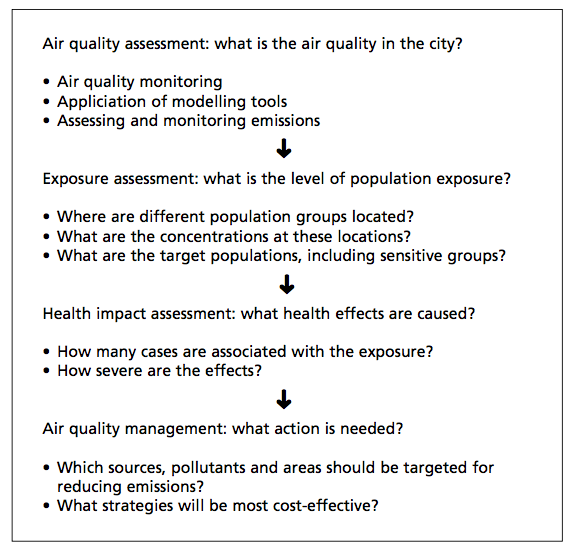
\includegraphics[width=0.7\textwidth]{Rationale_for_air_quality_monitoring}
\caption{Rationale for air quality monitoring \citep{WHO2002ambientmonitoring}}
\label{rationaleformonitoring}
\end{figure}

%This paper was instrumental in raising awareness of the need for air quality monitoring. 

Air pollution is formed up of gases and microscopic particles, which are often invisible to the naked eye. Therefore, in order for any pollution reduction strategies to be effective, there needs to be a method of measuring and monitoring air pollution so that problem areas can be identified.

A report by the \cite{WHO2002ambientmonitoring} looked at the importance of monitoring air quality for health impact assessment purposes. At the root of the rationale is identifying what the air quality is like in a given location. Second, the report details how the nature of population exposure must first be understood in the chain. Third, the population exposure needs to be assessed to understand the health impact. Finally, the health impact then should directly impact plans for air quality management and improving public health. This rationale is detailed is Figure \ref{rationaleformonitoring}.

Furthermore, the main pollutants that need to be monitored must be identified. Section \ref{airqualitymeasures} discusses these.
    
\section{Measures of air quality} \label{airqualitymeasures}

Many governments have central bodies that handle the measuring of air quality and the publishing of the readings so that the public can view them. In the UK, the Department for Environmental and Rural Affairs (DEFRA) are responsible for this and they release a yearly report on air quality statistics \citep{govuk2017airquality}, as well as daily and weekly readings on their official website \citep{defra2018website}. The data used for these are collected using the Automatic Urban and Rural Network (AURN) and the statistics focus on five main pollutants, detailed below in Table \ref{airqualityguidelines} These measurements make up the Daily Air Quality Index (DAQI), which is used to inform the public about the current or forecast risk of air pollution \citep{defra2018daqi}. Additionally, the \cite{eea2018airqualityindex} recently launched its own air quality index, which measures the same five pollutants. Both the UK and the EEA have air quality guidelines that specify a minimum air quality level that must not be exceeded. These are also detailed below in the table, with the more stringent limit taken in each case.

\nomenclature{DEFRA}{Department for Environmental and Rural Affairs}
\nomenclature{AURN}{Automatic Urban and Rural Network}
\nomenclature{DAQI}{Daily Air Quality Index}
\nomenclature{EEA}{European Environment Agency}


%\begin{enumerate}
%\item Fine particulate matter (PM\textsubscript{2.5})
%	\begin{enumerate}
%	\item 24-hour mean: \(50\mu g/m^3\) (not to be exceeded more than 35 times per year)
%    \item annual mean: \(40\mu g/m^3\)
%	\end{enumerate}
%\item Particulate matter (PM\textsubscript{10})
%	\begin{enumerate}
%    \item annual mean: \(25\mu g/m^3\)
%	\end{enumerate}
%\item Nitrogen dioxide (NO\textsubscript{2})
%	\begin{enumerate}
%	\item 1-hour mean: \(200\mu g/m^3\) (not to be exceeded more than 10 times per year)
%    \item annual mean: \(40\mu g/m^3\)
%	\end{enumerate}
%\item Ozone (O\textsubscript{3})
%	\begin{enumerate}
%	\item 8-hour mean: \(100\mu g/m^3\) (not to be exceeded more than 10 times per year)
%	\end{enumerate}
%\item Sulphur dioxide (SO\textsubscript{2})
%	\begin{enumerate}
%    \item 15-minute mean: \(266\mu g/m^3\) (not to be exceeded more than 35 times per year)
%	\item 1-hour mean: \(350\mu g/m^3\) (not to be exceeded more than 24 times per year)
%    \item 24-hour mean: \(125\mu g/m^3\) (not to be exceeded more than 3 times per year)
%	\end{enumerate}
%\end{enumerate}

\begin{table}[!tbp]
  \centering
  \small
  \caption{UK and EEA air quality guidelines}
  \label{airqualityguidelines}
  \begin{tabular}{ l l l l l l }
  \toprule
  & \multicolumn{5}{c}{Limit ($\mu g/m^3$)} 													\\ \cmidrule(l{0mm}r{0mm}){2-6}
  Gas/particulate  							& 15-minute 	& 1-hour 	& 8-hour 	& 24-hour 	& Annual 	\\ \midrule
  Fine particulate matter (PM\textsubscript{2.5}) 	& -- 			& -- 		& -- 		& 50 		& 40\textsuperscript{$\diamond$} 		\\
  Particulate matter (PM\textsubscript{10}) 		& -- 			& -- 		& -- 		& -- 		& 25 		\\
  Nitrogen dioxide (NO\textsubscript{2}) 			& -- 			& 200\textsuperscript{$\dagger$} 	& -- 		& -- 		& 40 		\\
  Ozone (O\textsubscript{3}) 					& -- 			& -- 		& 100\textsuperscript{$\dagger$}	& --		& -- 		\\
  Sulphur dioxide (SO\textsubscript{2})			& 266\textsuperscript{$\diamond$}		& 350\textsuperscript{$\ddagger$}	& --		& 125\textsuperscript{*}	& -- 		\\ \bottomrule
  \multicolumn{6}{l}{\textsuperscript{$\ast$}\footnotesize{Not to be exceeded more than 3 times per year}} \\
  \multicolumn{6}{l}{\textsuperscript{$\dagger$}\footnotesize{Not to be exceeded more than 10 times per year}} \\
  \multicolumn{6}{l}{\textsuperscript{$\ddagger$}\footnotesize{Not to be exceeded more than 24 times per year}} \\
  \multicolumn{6}{l}{\textsuperscript{$\diamond$}\footnotesize{Not to be exceeded more than 35 times per year}} \\
  \end{tabular}
\end{table}

%\nomenclature{SO\textsubscript{2}}{Sulphur dioxide}

In this study, we focus on particulates, nitrogen oxides and ozone. Further information about these pollutants is given below.

\subsection{Nitrogen oxides}

Nitrogen oxides (NO\textsubscript{x}) is a collective term for a group of reactive nitrogen-based substances that includes nitrogen monoxide (NO) and nitrogen dioxide (NO\textsubscript{2}). Research generally focuses on nitrogen dioxide because it one of the commonly regulated air quality pollutants \citep{Brook2004cardiostmnt}. In addition to this, NO rapidly oxidises with oxygen in the air to form NO\textsubscript{2} and so is not as prevalent in the environment. It also plays an important role in the formation of ozone (O\textsubscript{3}). One of the main sources of nitrogen oxides is the combustion of fossil fuels, which is typically found in petrol or diesel vehicles. Long-term exposure to NO\textsubscript{2} is associated with an increase in mortality rates \citep{Faustini2014nitrogenmortality}.

%\subsection{Sulphur dioxide}
%
%Sulphur dioxide (SO\textsubscript{2}) is a toxic gas with a pungent smell. It reacts with water to form sulphuric acid, which is a component of acid rain. Excluding anthropogenic sources of sulphur dioxide, the gas is typically found in low quantities in the environment (around 1 part-per-billion (ppb)), meaning the majority is a by-product of human activity. It is mainly produced by combusting sulphur-containing fossil fuels and is, therefore, a good indicator of air pollution attributable to motor-vehicles and industrial factories. Elevated levels of SO\textsubscript{2} has been associated with widespread illness, although this may be due to its role in the formation of particulate sulphates \citep{Brook2004cardiostmnt}. Other studies have shown that it has adverse health effects \citep{pope1995particulate,pope2002lungcancercardiomortality}.

\nomenclature{ppb}{Parts-per-billion}

\subsection{Ozone}

Ozone (O\textsubscript{3}) is another pungent gas that is highly reactive. More specifically, ozone that is classed as a pollutant is known as `tropospheric ozone' as it is found near ground-level. Low-level exposure is widespread as it is formed naturally in the atmosphere. In addition to this, the action of solar UV radiation on NO\textsubscript{x} leads to the formation of O\textsubscript{3}, meaning concentrations are generally higher on sunnier days \citep{Brook2004cardiostmnt}. O\textsubscript{3} is a known pulmonary irritant \citep{Ebi2008ozonePMhealth} and long-term exposure to ambient ozone is related with an increased risk of respiratory and circulatory mortality \citep{Turner2016ozonemortality}.

\subsection{Particulates}

Particulates or particulate matter (PM) are mixtures of solid matter and liquid matter that are suspended in the air. They come in various sizes, of which the standard measures are PM\textsubscript{1}, PM\textsubscript{2.5} and PM\textsubscript{10}. These refer to the measured quantity of particles with size \textless \SI{1}{\micro\metre}, \textless \SI{2.5}{\micro\metre} and \textless \SI{10}{\micro\metre}, respectively. PM is created in two ways: (i) by direct emission, or (ii) by the physicochemical transformation of gases \citep{Brook2004cardiostmnt}. Inhalation of PM\textsubscript{2.5} and PM\textsubscript{10} is associated with many adverse health outcomes \citep{pope1995particulate,pope2002lungcancercardiomortality,Anderson2012clearingtheair,Beelen2014escapeproject}.

\nomenclature{PM}{Particulate matter}

    
\section{Monitoring urban air quality}

Given the serious health implications of air pollution detailed in Section \ref{healthimpact} and the prevalence of minimum air quality regulations around the world, air quality monitoring is of utmost importance, particularly in urban environments where pollution is often highest. To get a distributed measurement of air pollution in an area, multiple devices are often deployed. The geographical distance between these devices affects the \textit{spatial} resolution of the air quality data, whilst the repeated collection of measurements from the same location affects the \textit{temporal} resolution.

\subsection{Previous monitoring devices}

There are a large number of different air quality monitoring devices detailed in the literature. They use a variety of different computers upon which the sensors are based, as well as containing sensors for measuring a number of different gases and particulates. These devices are either deployed in a fixed location, or they are attached to different vehicles for taking non-static measurements. Table \ref{listofprevdevices} provides a comprehensive overview of air quality monitoring devices in the literature, detailing the vehicle used, which gases and/or particulates were measured and what computer the device was based on. Particularly relevant studies in this table are discussed below.

One example of an air quality monitoring device is an Arduino-based device deployed on a public transport bus fleet \citep{2014busairqualityVSN}. They built a network of these devices, called a Vehicular Sensor Network (VSN). Each device communicated its air quality measurements to fixed access points via radio, and then these forward the data on to a central server. The authors found that using only a few vehicles with these monitoring devices attached, they could monitor a whole city of size \(160km^2\). This paper is interesting in the fact that it presents the current air quality monitoring system of the analysed city, before explaining how a network of mobile sensors could improve the monitoring. 

\nomenclature{VSN}{Vehicle sensor network}

Other public transport has been used to attach air quality monitoring devices. \cite{Hasenfratz2015highresmapsTram} attached monitoring devices to trams in Zurich, Switzerland, and collected measurements over a two-year period. By using the tram network, they were able to cover a large urban area of 100km\textsuperscript{2} on a regular basis. For the base computer of their device they used a Gumstix, which is similar to a Raspberry Pi.  The device itself stored measurements in a local database and transmitted them in real-time over a cellular network, before then deleting stored readings once receipt was confirmed. Again, the paper highlighted the advantage of this mobile system compared to a static government monitoring station. Furthermore, their novel contribution was to derive a cost function for all street segments of Zurich's road network, which was then incorporated into a route finding algorithm to compute the health-optimal path. This was then compared to the route generated without the inclusion of this cost function and the authors found that taking the health-optimal path led to a 7.1\% reduction in particulate pollution exposure. \cite{Hagemann2014aerotram} also used trams to assess spatial variability of particle number concentrations and NO\textsubscript{x}.

Another study used a device attached to a bicycle, named Aeroflex \citep{Elen2013aeroflex}. The focus was on high adaptability and ease of use since everybody is `able to ride a bike', thus enabling any volunteer member of the public to contribute to air quality monitoring. This ease of use was not only for the bicycle, but also for the software that collected, sent and displayed the data. All of the air quality monitoring equipment was attached to the bicycle (see Figure \ref{aeroflex}), including a robust data transmission system that could provide real time measurements on air quality. The Aeroflex took measurements every second and was ridden around a set route multiple times in order to provide a high spatial resolution and to ensure good temporal resolution. The success of the project was demonstrated by city authorities using it in a number of cities in Belgium, including Antwerp, Ghent and Brussels. Whilst the novel use of a bicycle to monitor air quality is a major advantage of this study, it only focused on measuring particulates, carbon monoxide and black carbon. Out of these, only particulates are part of the indexes used by the UK and the EEA, which questions the device's usefulness in helping the city authorities in monitoring air quality so that air pollution limits are not broken. This identifies a gap in the literature for a bicycle-based monitoring system that measures more of the gases and particulates detailed in Section \ref{airqualitymeasures}.

\begin{figure}[!htb]
\centering
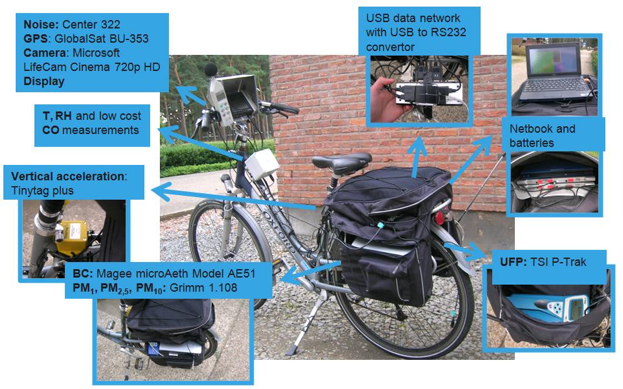
\includegraphics[width=0.7\textwidth]{aeroflex}
\caption{Aeroflex air quality monitoring platform developed by \cite{Elen2013aeroflex}}
\label{aeroflex}
\end{figure}

Another interesting study was conducted by \cite{Apte2017googlestreetview} using Google Street View cars in California. The study covered 24,000km within a 30km\textsuperscript{2} area, meaning it had much higher spatial and temporal resolutions than previous mobile monitoring studies. By also incorporating this data with Google Street View's imagery, it was possible to analyse `hotspots' and suggest plausible causes of the problem, thus making the dataset richer. For example, a metal recycling business was identified to be the cause of a hotspot for black carbon, nitrogen oxide and nitrogen dioxide. Having this level of detail would greatly help in informing council decision-making relating to air pollution. The authors also note that having routine availability of high-resolution air quality data in cities could make it possible to alter personal behaviour, much like real-time traffic data currently affects driving decisions. However, the study used industry-grade monitoring equipment instead of a low-cost device. Whilst this is feasible for a company such as Google, this is not conducive to making low-cost monitoring widespread. 

Looking at the air quality monitoring literature as a whole, a number of areas remain unaddressed. Firstly, no study measure all of pollutants detailed in Section \ref{airqualitymeasures} that form UK and EU legislation. Whilst this may be because it is difficult to fit that number of sensors into one device, if mobile air quality monitoring in the future is to be a viable option in the UK, this needs to be addressed. Secondly, the capabilities of using a sole Raspberry Pi device for air quality monitoring purposes needs further investigation as it is often used in conjunction with another computer (see Table \ref{listofprevdevices}). Thirdly, only three of the studies detailed in Table \ref{listofprevdevices} used bicycles, which are ubiquitous, non-polluting vehicles that would appear to be an ideal candidate vehicle for mobile air quality monitoring. Finally, in all of these three cases, the air quality monitoring device appeared bulky and cumbersome (see Figure \ref{aeroflex} for an example). Therefore, it would be interesting to see if all of the sensing capabilities could be incorporated into a small device.

\newgeometry{left = 3cm, right = 3cm, top = 4cm, bottom = 2cm}

\begin{landscape}
  \small
\begin{longtable}{ p{0.4\textwidth} p{0.3\textwidth} p{0.4\textwidth} p{0.2\textwidth} }
  \caption{\mbox{List of air quality monitoring devices in the literature}}
  \vspace{-0.4cm}
  \label{listofprevdevices} \\
  %\renewcommand{\arraystretch}{0.5} \\
  \toprule
  Study & Vehicle type & Gas/particulates measured & Base computer \\ \midrule
  \cite{Jabbar2017bikefossarchitecture} & Tricycle & PM\textsubscript{2.5} & RPi \\ \midrule
  \cite{Alvear2016ecosensor} & Bicycle & CO\textsubscript{2}, O\textsubscript{3} & RPi \& Waspmote\\ \midrule
  \cite{Apte2017googlestreetview} & Car & BC, NO, NO\textsubscript{2} & Aclima Ei \\ \midrule
  \cite{Devarakonda2013} & Bus \& Car & CO, PM & Arduino \\ \midrule
  \cite{Elen2013aeroflex} & Bicycle & PM\textsubscript{1}, PM\textsubscript{2.5}, PM\textsubscript{10}, BC, CO & Netbook \\ \midrule
  \cite{Ferdoush2014rasppiandarduino} & Stationary & Temperature, humidity & RPi \& Arduino \\ \midrule
  \cite{Hagemann2014aerotram} & Tram & CO, CO\textsubscript{2}, NO, NO\textsubscript{x}, O\textsubscript{3}  & Custom \\ \midrule
  \cite{Hagler2010durhamallelectric} & Electric car & CO, UFPs & N/A \\ \midrule
  \cite{Hasenfratz2015highresmapsTram} & Tram & O\textsubscript{3}, CO, NO\textsubscript{2}, UFPs & Gumstix \\ \midrule
  \cite{Hoang2013hanoihexagons} & Motorcycle & CO & Waspmote \\ \midrule
  \cite{Peters2013cycleruns} & Bicycle & PM\textsubscript{10}, UFP & N/A \\ \midrule
  \cite{Piedrahita2014quantexposuremtrng} & Person (wearable) & CO, CO\textsubscript{2}, NO\textsubscript{2}, O\textsubscript{3} & Arduino \\ \midrule
  \cite{2014busairqualityVSN} & Bus & NO\textsubscript{2}, CO\textsubscript{2}, CO, O\textsubscript{3} & RPi \& Arduino \\ \midrule
  \cite{sun2016HKmarathonML} & Stationary & CO, NO\textsubscript{2}, O\textsubscript{3}, PM\textsubscript{2.5} & Arduino \\ \midrule
  \cite{Wallace2009mobilehamilton} & Van & NO\textsubscript{x}, SO\textsubscript{2} & N/A \\ \midrule
  \cite{Weijers2004movingmeasurementunit} & Van & PM\textsubscript{1}, PM\textsubscript{\textgreater 1} & N/A \\ \midrule
  \cite{Westerdahl2005losangeles} & Car & CO, CO\textsubscript{2}, PM\textsubscript{2.5}, NO, NO\textsubscript{2} & N/A \\ \midrule
  \cite{Wong2009envmonitoringtemporal} & Car & CO, NO\textsubscript{x} & Renesas MCU \\ \bottomrule
  \hline
\end{longtable}

\end{landscape}

\restoregeometry

\nomenclature{CO}{Carbon monoxide}
\nomenclature{UFP}{Ultra-fine particle}
\nomenclature{BC}{Black carbon}
\nomenclature{RPi}{Raspberry Pi}

\subsection{Spatial variability}

A number of studies have shown that air pollution in cities can vary over extremely short distance ($ < 100$~m) [REFs]. Therefore, air pollution measurements from a fixed monitoring station are likely only representative of a small radius around the site. This acts as a trade-off with the improved accuracy that fixed monitoring stations provide. Furthermore, with these stations typically located in areas of high pollution that the local authorities wish to monitor, the measurements may provide an inflated estimate if taken to be representative of a large area.

It has also been noted that the presence of unbroken rows of tall buildings on either side of a road can trap air pollution. These types of roads have been named `street canyons'. In addition, some evidence suggests that the level of pollution behind these buildings can drop to background levels, indicating the dramatic variability in pollution that can occur in a city.

\subsection{Spatial resolution} \label{spatialres}

When monitoring air quality, a higher spatial resolution is considered to be better because air quality can be mapped in greater detail and exact problem areas identified more easily.

Air pollution is typically measured mainly using a network of fixed monitoring stations \citep{Adams2012hamilton20052010}. Since they are fixed, they can be attached to a consistent power source and can include an array of measuring equipment that can measure a wide variety of pollutants with a level of accuracy that is often not possible on smaller, portable devices. However, these stations are likely to be placed in locations with high levels of air pollution \citep{Kanaroglou2005location} so that accurate measurements can be taken to ensure pollution regulation limits are not broken. The high cost and maintenance of these stations also means that only a low number can be built and deployed \citep{Devarakonda2013}, which leads to two possibilities arising: (i) a smaller area is covered with higher spatial resolution, or (ii) a larger area is covered with lower spatial resolution. In either case, the spatial resolution remains poor due to the low overall number of deployed devices.

Conversely, a monitoring device attached to a moving vehicle -- i.e. a \textit{mobile} device -- can cover a larger area for a lower cost since a much smaller number of devices needs to be used \citep{Wallace2009mobilehamilton}. The area being monitored is also flexible as a moving device does not have the same restrictions as a fixed one. Moreover, setting a suitably short interval for taking air quality measurements enables the moving device to have a greater spatial resolution as many measurements can be taken in close proximity to one another. For example, \cite{Apte2017googlestreetview} took measurements every 30 metres and found using a mobile system led to a $10^4$ to $10^5$ times greater -- i.e. finer -- spatial resolution compared to fixed monitoring stations. These improvements do come at a cost, however. Temporal resolution is reduced because any given location will only have multiple measurements once the moving device visits that exact location again \citep{Wong2009envmonitoringtemporal}. One solution to this problem is to increase the number of vehicles deployed with the monitoring device attached.

The apparent advantages of mobile air quality monitoring over static monitoring and its increasing prevalence in the literature suggest it is more suitable for this project. In addition, \cite{Kuhlbusch2014futureEUair}, in a collective statement about the future of European air quality monitoring, recommend mobile devices for `the collection of highly spatially and temporally resolved data'.

\subsection{Temporal resolution}

Much of the air quality literature relating to the resolution of measurements focuses on the spatial resolution. However, the temporal resolution is also important as higher temporal resolution allows one to better understand how the pollution in an area changes over time.


\section{Comparison of single-board computers}

Whilst this section does not intend to provide a comprehensive comparison of single-board computers (SBCs) for use in this project (this would be a significant project itself), it is worth considering the relative advantages and disadvantages of various SBCs.

\nomenclature{SBC}{Single-board computer}

The decreasing cost and size of computers over time has created a market for low-cost, single-board computers that are compact, but have significant computing capabilities. There are many different makes of SBCs available, but the most commonly used SBCs in the air quality monitoring literature are compared in this section. Whilst an Arduino is technically a microcontroller unit (MCU), its prevalence in the literature means it should also be included in this comparison.

\nomenclature{MCU}{Microcontroller unit}

\subsection{Raspberry Pi (RPi)}

Due to the small size and low-cost of Raspberry Pis, they are viewed as an ideal computer to run an air quality monitoring device. These SBCs do not come with any sensing capabilities built-in, meaning either sensors need to be attached or a separate circuit board containing the sensors needs to be connected to the RPi. Table \ref{sbccomparisontable} shows the details of four popular RPi models. Only the RPi 3 and RPi Zero W have Wi-Fi and Bluetooth capabilities, which would be useful in this kind of project for transferring data from the monitoring device. In addition, the RPi 3 has greater computational power, but requires substantially more power and costs over three times as much. The RPi Model A+ and RPi 2 have no clear merit over the other two RPis, suggesting using a RPi 3 or RPi Zero W would be sensible.

Raspberry Pis have been used in air quality research previously \citep{ibrahim2015IOTenvmon,Balasubramaniyan2016AQMS_RPi,Rahman2017adaptivesensingRPi,thorpe2017RPimesh,alkandari2018airqualityexperimental}, with one study attaching them to public buses \citep{2014busairqualityVSN} and another using them as part of tricycle-based mobile system \citep{Jabbar2017bikefossarchitecture}. The use of Raspberry Pis in these studies confirms its suitability for air quality monitoring.

There are a variety of Raspberry Pi models available, with an apparent trade-off between size and power consumption and computing power. \cite{thorpe2017RPimesh} used both the Raspberry Pi 3 Model B and the Raspberry Pi Zero W for particulate sensing devices and found the former to have a much more reliable WiFi signal. However, the distance between devices was up to 30 metres and the Raspberry Pi used in this project will not be subjected to sending data over such distances given the whole system will be installed on one vehicle. This suggests the RPi Zero W may be suitable.
   
One issue that Raspberry Pis have is that they do not have an onboard clock and so the system time is the time since the last boot. To alleviate this problem, a time source is needed to accompany the RPi.

Furthermore, the type of sensors being used in this project output an analog signal, which the RPi cannot read directly. As a result, an analog-to-digital converter (ADC) would need to be fitted to the sensor board.

\subsection{Arduino}

An Arduino is a single-board microcontroller motherboard which has been widely used in the environmental monitoring literature \citep{2014busairqualityVSN,Devarakonda2013,Balasubramaniyan2016AQMS_RPi,sun2016HKmarathonML,Ferdoush2014rasppiandarduino,Lee2014arduinorestful,Alvear2016ecosensor,Fuertes2016realtime,Piedrahita2014quantexposuremtrng,Abraham2014costeffindoor}. The hardware is open source with a large community of support and the software is open source, too. Since it is a microcontroller, it can only run one program at a time. Whilst its CPU speed from Table \ref{sbccomparisontable} seems low, a microcontroller is not comparable to the SBCs in this respect and so this type of comparison should be avoided. Despite this, a microcontroller is good for simple, repetitive tasks and as a result, is considered to have relatively fast computation. Moreover, Arduinos read analogue inputs, which is beneficial since sensors typically output an analogue signal. However, an Arduino is unsuitable for multiple, complex tasks that require more than one program to be run. Furthermore, an Arduino does not come with built-in Wi-Fi or Bluetooth (see Table \ref{sbccomparisontable}), meaning an additional dongle would be needed.

\subsection{BeagleBone}

The BeagleBone is a low-cost, community supported SBC that runs Linux. It has been used successfully in air quality monitoring studies, including a study in which it was part of a \textit{real time} air quality monitoring system \citep{Min2014airfeedbeagle}. The BeagleBone passed measurements on to a web interface using a Wi-Fi connection, but had an additional local SQLite database as backup in order to mitigate variations in Wi-Fi signal. The authors also connected an LCD screen to the BeagleBone in order to aid with the usability of the device. In a different study by \cite{Desai2017beagleboneblack}, the BeagleBone stored comma-separated value (CSV) files containing the day's measurements, which were then uploaded to a cloud-based database at the end of the day. 

The device itself is almost twice the price of the second-most expensive SBC in Table \ref{sbccomparisontable} and has the highest power requirement. It also only has the same computational power as the RPi zero W, which is a smaller and cheaper device. However, it does have built-in Wi-Fi and Bluetooth, which would be beneficial.

\subsection{Comparison} \label{sbccomparison}

\begin{table}[!htbp]
  %\centering
  \footnotesize
  \caption{Comparison of SBCs}
  \label{sbccomparisontable}
  \begin{tabular}{ l p{0.175\textwidth} p{0.15\textwidth} l p{0.07\textwidth} p{0.06\textwidth} p{0.1\textwidth}}
  \toprule
  Model & Recommended / min. current\textsuperscript{4} & CPU speed & RAM & Wi-Fi & Blue--tooth & Price \\ \midrule
  RPi Model A+ & 700mA/180mA & 0.7GHz & 512MB & No & No & \textsterling 20.00\textsuperscript{1} \\
  RPi 2 Model B & 1.8A/350mA & 0.9GHz (QC) & 1GB & No & No & \textsterling 34.00\textsuperscript{1} \\
  RPi 3 Model B & 2.5A/400mA & 1.2GHz (QC) & 1GB & Yes & Yes & \textsterling 32.00\textsuperscript{1} \\
  RPi Zero W & 1.2A/150mA & 1GHz & 512MB & Yes & Yes & \textsterling9.16\textsuperscript{1} \\
  Arduino Uno & 100mA/50mA & 16MHz & N/A & No & No & \textsterling 16.64\textsuperscript{2} \\
  BeagleBone Black & 1.2A/500mA & 1GHz & 512MB & Yes & Yes & \textsterling 62.24\textsuperscript{3} \\ \bottomrule
  \multicolumn{6}{l}{\textsuperscript{1}\footnotesize{Source: \href{https://thepihut.com/collections/raspberry-pi}{https://thepihut.com/collections/raspberry-pi}}} \\
  \multicolumn{6}{l}{\textsuperscript{2}\footnotesize{Source: \href{https://store.arduino.cc/}{https://store.arduino.cc/}}} \\
  \multicolumn{6}{l}{\textsuperscript{3}\footnotesize{Source: \href{https://beagleboard.org/black-wireless}{https://beagleboard.org/black-wireless}}} \\
  \multicolumn{6}{l}{\textsuperscript{4}\footnotesize{All require 5V, except the Arduino Uno which requires 7-12V. }} \\
  \multicolumn{6}{l}{\footnotesize{(QC) indicates that the CPU is quad-core.}} \\
%  \hline
  \end{tabular}
\end{table}

Given the greater usage of the Raspberry Pi and Arduino in the literature (see Table \ref{listofprevdevices}), it would be sensible to also use one of these devices for this project. The Arduino has the advantage of a lower power consumption and can read signals from the sensors without the need of an ADC chip. However, it is a microcontroller and so does not have the same computational capabilities or flexibility as the RPi. Comparing all of the different RPi models, the RPi 3 and the RPi Zero W seem the most sensible options. They both have built-in Wi-Fi and Bluetooth capabilities. The RPi 3 also has the greatest computation power, but costs the most out of the RPis. The RPI Zero W is not as powerful, but requires the least power to run and has the lowest cost by far. For the above reasons and the university's availability of the Raspberry Pi in this project, it would be sensible to use either an RPi 3 or RPi Zero W.

\nomenclature{ADC}{Analog-to-digital converter}


\section{Power} \label{power}

The comparison of SBCs in Section \ref{sbccomparison} concluded that either the Raspberry Pi 3 or Zero W would be the most suitable SBC to base the sensing device on for this project. Consequently, this section focuses on powering a Raspberry Pi.

\subsection{Raspberry Pi power requirements}

% The current requirement is dependent on the model, but 2.5A is recommended \citep{rpi2018powerfaq}. 

A Raspberry Pi requires a 5V power source that connects via micro-USB. Table \ref{sbccomparisontable} shows the current requirements for different Raspberry Pi models. The RPi Zero W has the lowest power needs of the compared models with a minimum required current of 150mA. The RPi 3 requires 400mA at a minimum. However, these are optimistic figures as it is likely that extra current will be needed to also provide power to the sensing board, which will hold the air quality sensors. Considering the aforementioned values, the absolute minimum power needed would be 0.75W (0.15A $\times$ 5V).

\nomenclature{HAT}{Hardware-on-top}

%\begin{table}[!htbp]
%  %\centering
%  \caption{Raspberry Pi power requirements by model \citep{rpi2018powerfaq}}
%  \label{pipowertable}
%  \begin{tabular}{ p{0.3\textwidth} p{0.3\textwidth} p{0.3\textwidth} }
%  \toprule
%  Model & Recommended PSU current capacity & Typical bare-board active current consumption %\\ \midrule
%  Raspberry Pi Model A+ & 700mA & 180mA \\
%  Raspberry Pi 2 Model B & 1.8A & 350mA \\
%  Raspberry Pi 3 Model B & 2.5A & 400mA \\
%  Raspberry Pi Zero W & 1.2A & 150mA \\ \bottomrule
%  \hline
%  \end{tabular}
%\end{table}

\subsection{Power sources}

For vehicle-based devices, an implicit requirement is that the power source must be portable. There are two main options that appear viable to satisfy such a requirement: (i) battery-based, and (ii) energy harvesting.

A battery pack could provide the power for a Raspberry Pi as long as the voltage was 5V. Four AA batteries could provide 6V (1.5V each) and then a voltage regulator could be used to reduce this down to 5V to meet the Pi's requirement. This is a simple solution that would be reliable and provide consistent power.

The second option is to use some form of energy harvesting from the vehicle the device is attached to. These techniques would be useful for making a self-sustaining monitoring system. One example is to use the weaving motion of a bicycle whilst the user is cycling. \cite{Yang2012weaving} studied this form of energy harvesting, but found that it only produced 6.6mW, which is far too low for powering a Raspberry Pi. Another study by \cite{hui2011energyharvestingbicycle} found that using a tyre-driven dynamo could generate power in the range 7-15W. This would be easily sufficient to power a RPi and is a potentially viable option. Other energy harvesting techniques include using the vibrations to generate piezo-electricity or generating energy via solar panels. However, even if it is possible to generate enough current to run the RPi, this current needs to be produced constantly in order to run the device. Vehicles are prone to stopping in traffic and at junctions, which would lead to the generating current cutting out. To solve this problem, a capacitor would need to be included in the circuit for storing energy. There are also cost implications of including a dynamo. Given batteries are a low-cost and readily available power source for the RPi that can provide consistent power, they seem the more sensible option.

%In both cases it is currently unclear whether they will provide enough power and how long they will be able to supply sufficient power for. Therefore, testing is required to identify which power source is most suitable.

Furthermore, it is critical that the power source can provide energy for a suitable amount of time so that a sufficient number of measurements can be collected. Again, energy harvesting compares poorly to a simple battery solution as it needs to harvest and store the energy as the user cycles. Standard AA batteries have a capacity of between 600 and 2850mAh\footnote{Source: \href{https://en.wikipedia.org/wiki/AA_battery}{\url{https://en.wikipedia.org/wiki/AA_battery}}}, which is enough to power a RPi Zero W with a current draw of 150mA for between 4 and 19 hours.

For the above reasons, it is apparent that energy harvesting is not practical as a power source in this project. Therefore, it is not considered further.

%\subsection{Automatic shutdown capability}

%The power supplied to the RPi also needs to be stable. If the power falls below the required level for the RPi, then improper shutdown can result in corruption of the SD card and loss of data. To help solve this issue, a regulated circuit can be used to provide an uninterruptible power supply (UPS).

%\nomenclature{UPS}{Uninterruptible power supply}



\section{Use of low-cost sensors} \label{lowcostsensors}

The recent emergence of low-cost sensors as alternatives to high-cost sensors such as the DustTrak 8530, which costs around \textsterling 8,000, has enabled low-cost and widespread monitoring of air quality that was previously only carried out by professional personnel. Historically, professional training has been required to operate the equipment and regular maintenance is needed in order to ensure high data quality and accuracy. These tasks can be avoided by using the low-cost sensors.

However, a major problem is that the data generated by these low-cost sensors is often of questionable accuracy and reliability. The causes of this are varied \citep{Clements2017lowcostworkshop}. Firstly, low-cost sensors are often sensitive to   environmental conditions such as humidity and temperature. Secondly, the sensor readings are known to change as they age, with sensor drift leading to the frequent need to recalibrate, thus reducing their cost advantage. Furthermore, they are sensitive to the air flow, which is particularly poignant given the prevalence of mobile air quality monitoring deployments. Finally, the low-cost sensors can be exhibit a delayed response to a change in the pollution level and a sensor for one pollutant can exhibit cross-sensitivity to a variety of other pollutants. As a result of these issues with low-cost sensors, calibration techniques have been developed to help improve the data quality.

\subsection{Calibration of sensors}

Calibration of sensors is key to ensuring that accurate and reliable measurements are obtained. This topic has particular gravitas for low-cost sensors because of their lower accuracy than more expensive alternatives.

%In 2008, the \cite{eudir2008airquality} issued a directive on ambient air quality and cleaner air in Europe, in which it laid out a set of Data Quality Objectives (DQOs) that specify the maximum level of acceptable uncertainty in air quality measurements. These are detailed in Table \ref{dataqualityobjectives}. If low-cost sensors are to be a viable for meaningful air quality monitoring, their measurements will need to meet or surpass these DQOs.
%
%\nomenclature{DQO}{Data Quality Objective}
%
%\begin{table}[!htbp]
%  \centering
%  \caption{EU Data Quality Objectives}
%  \label{dataqualityobjectives}
%  \begin{tabular}{ l c}
%  \toprule
%  Gas/particulate & Maximum uncertainty \\ \midrule
%  CO & 25\% \\
%  NO\textsubscript{2} & 25\% \\
%  SO\textsubscript{2} & 25\% \\
%  PM\textsubscript{2.5} & 50\% \\
%  PM\textsubscript{10} & 50\% \\
%  O\textsubscript{3} & 30\% \\ \bottomrule
%  \end{tabular}
%\end{table}

One simple calibration technique is to calibrate each sensor to a `ground truth' measurement from a more expensive sensor. One study calibrated low-cost particulate sensors using a device 400 times more expensive and found the sensor provided an accuracy of over 90\% \citep{thorpe2017RPimesh}. Typically, linear regression has been used for sensor signal normalisation to reference measurements. However, there is no evidence that these correlations are transferable to different locations \citep{Clements2017lowcostworkshop}. Furthermore, the study by \cite{thorpe2017RPimesh} was conducted indoors and in a controlled environment, which does not involve the same difficulties as outdoor air quality monitoring using low-cost sensors. Indeed, linear calibration models developed in a laboratory environment have been shown to perform poorly on ambient data \citep{Castell2017}.

[REWRITE] To counter these problems, multi-variate linear regression models have been used \citep{Spinelle2015fieldcalibrationa,Spinelle2017fieldcalibrationb}, which provide an improvement to the calibration because they take into account more complex factors that are known to affect sensor performance. They also tested artificial neural network (ANN) calibration. ANNs are a supervised machine learning technique that trains the model on known input-output pairs and then uses the trained model to predict the output from unseen inputs. The authors found in both papers that multi-variate linear regression had the highest measurement uncertainty along with the simple linear regression model when compared to an artificial neural network (ANN) for calibration of NO, NO\textsubscript{2}, CO, CO\textsubscript{2} and O\textsubscript{3} sensors. Despite the high uncertainty, it was still possible to exceed the DQO for O\textsubscript{3} using a linear regression model. In addition, the ANN approach resulted in exceeding the DQOs for O\textsubscript{3} and CO, and generated an extremely low uncertainty level for CO\textsubscript{2} even though this gas does not have a DQO. On the other hand, meeting the NO and NO\textsubscript{2} DQOs remained a challenge, which may have been as a result of their high cross-sensitivity. Therefore, despite this supervised machine learning technique providing more effective calibration than linear or multi-variate linear regression, further work is needed to calibrate sensors so they comply with the DQOs.

\nomenclature{ANN}{Artificial neural network}

%More recently, machine learning has been used to improve low-cost sensor performance \citep{zimmerman2018machinelearning,sun2016HKmarathonML,Spinelle2015fieldcalibrationa}, although the technique is still in its infancy. One way these techniques work is by clustering measurements into clusters, which are groups of similar data points. These clusters can then be used to more accurately/reliably identify where air pollution significantly varies in an area.

Another machine learning technique uses random forest-based machine learning algorithm. \cite{zimmerman2018machinelearning} were the first to apply this technique to low-cost air quality sensor calibrations. Again, it was found that a machine learning technique (random forests) outperformed multivariate linear regression models and was able to make the low-cost sensors accurately characterise air pollution concentrations synonymous with European city levels. Moreover, by including measurements of additional pollutants, the random forest model was able to account for pollutant cross-sensitivities, which \cite{Spinelle2015fieldcalibrationa,Spinelle2017fieldcalibrationb} struggled with. This highlights the need of having multiple sensors in the same device.

Whilst it appears machine learning methods are the best available methods for low-cost sensor calibration, the aforementioned studies were used stationary air quality monitoring. Thus, it is unclear how these methods would perform when calibrating in near real-time. This should be investigated further.



\subsection{Air flow} \label{air_flow}

Since low-cost sensors are sensitive to the air flow, it is important that the sensors are provided with a consistent air flow so as to not affect their measurements.

One study has noted the benefit of air flow in improving air quality measurements from low-cost sensors. \cite{thorpe2017RPimesh} found that the increased air flow from using an integrated fan improved the signal to noise ratio of a particulate sensor. The fan provided a more consistent air flow to the sensor, which may have been the reason for the improvement. However, the author noted that battery draining may have led to a variable fan speed, which in turn could have affected the measurements. Thus, variability in air flow would need to be controlled for in any modelling.

In addition, \cite{Hasenfratz2015highresmapsTram} used a fan installed in the back of their air quality monitoring `box' to draw air out and ensure a steady air flow.

An alternative to using a fan for improving air flow is to funnel the air flow directly onto the sensor. This could be achieved through the use of a cone-shaped device. Unfortunately, a literature search did not discover any research relating to this application. Therefore, this should be researched further.



%\section{Data display}

%In order for air quality data to be accessible to a wide range of people, it needs to be displayed in a way that is easy to understand and interpret. The process of displaying the data can be separated into two distinct parts. Firstly, the technology for displaying the data needs to be considered. For example, ... Secondly, it is important to consider what is the best way of mapping the air quality data. Both of these parts are discussed below.

\section{Mapping air pollution} \label{mappingpollution}

Given the health impact of air pollution detailed in Section \ref{healthimpact}, maps are needed to identify pollution `hot spots', to show changes in pollution over time, to define at-risk groups and to provide better air pollution exposure estimates for epidemiological studies.

\subsection{Colouring}

In the UK, the recommended air quality index is the Daily Air Quality Index (DAQI). For each of the pollutants that are officially monitored in the UK (Section \ref{airqualitymeasures}), the DAQI is indexed 1-10 and is divided into four bands: low, moderate, high and very high. It was designed to inform the public about air quality in a simple and easy to understand way. An example is shown in Figure \ref{fig:daqi_pm10}, which is for PM10.

\begin{figure}[!htb]
\centering
\includegraphics[width=\textwidth]{images/daqi_pm10}
\caption{DAQI for PM10 \citep{defra2018daqi}.}
\label{fig:daqi_pm10}
\end{figure}

The DAQI levels can be used to colour pollution maps. For example, a PM10 measurement of 56~$\mu g/m^3$ would be coloured yellow. By doing this, the generated pollution maps are relevant and consistent with the rest of the UK's air quality information.

\subsection{Estimation techniques} \label{estimationtechniques}

As discussed in Section \ref{spatialres}, current air quality monitoring mainly uses fixed monitoring stations. Even in the 1990s, it was noted that air pollution often varies over extremely short distances whilst the air quality data from these fixed stations are often sparse, leading to highly generalised maps and poor estimates \citep{Briggs1997mappingGIS}.

As a result, techniques have been developed to generate estimated air pollution values in areas where no readings have been taken, thus allowing the improvement of air pollution maps by increasing the resolution. Such methods include spatial interpolation, dispersion modelling and regression-based approaches. A specific example of a regression-based approach is land-use regression (LUR), which was first detailed by \cite{Briggs1997mappingGIS} using data from the SAVIAH (Small Area Variations in Air Quality and Health) study. It has become increasingly popular since its introduction \citep{Hoek2008LUR}. This method combines air quality measurements spread over an area with stochastic modelling in order to generate air quality predictions at unsampled locations. The independent variables for the regression are obtained through geographical-information systems (GIS), which contains data on various environmental factors such as traffic volume and the road network. Figure \ref{LURexplanation} visually demonstrates this method. $y$ is the pollution concentration and $x_i$ are the land-use types within the `buffer' (circles). Good performance of the regression maps was achieved, with $r^2$ values ranging from 0.79 to 0.87 across the three mapped locations. However, LUR models are poor at separating out the impact of different pollutants due to the high correlation that can occur between pollutants \citep{Hoek2008LUR} and this type of extrapolation can perform poorly when the study area has significantly different land-use. For example, moving the study area from Bath, which is a small city in the countryside, to London, which is a much bigger and congested city.

\begin{figure}[!tb]
\centering
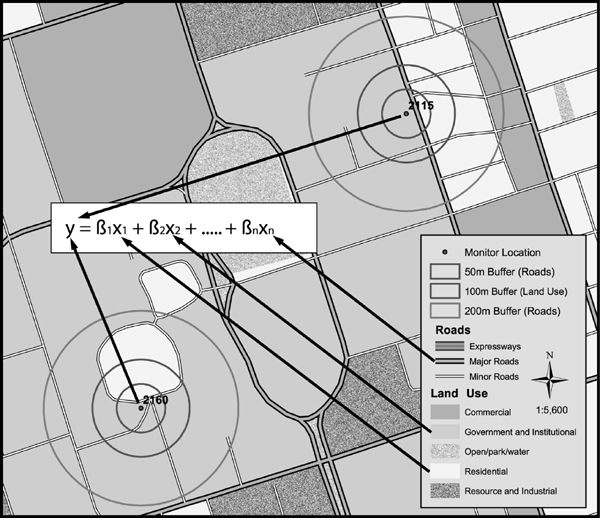
\includegraphics[width=0.7\textwidth]{LURexplanation}
\caption{Visual representation of LUR by \cite{Jerrett2005evalmapmodels}.}
\label{LURexplanation}
\end{figure}

%GIS files are made publicly available from DEFRA for modelling purposes for local air quality management. The relevant file could be incorporated with the data obtained in this project to generate pollution maps of the local area that includes unsampled locations.

\nomenclature{GIS}{Geographical-information system}
\nomenclature{LUR}{Land-use regression}

\subsection{Mapping visualisations}

A particularly interesting visualisation of geo-located air quality data is a heatmap. Google's API has a built-in Heatmap Layer for client-side rendering of heatmaps, which can be used to visualise data in this way. Figure \ref{heatmap} shows an example from their website. 

\nomenclature{API}{Application programming interface}

\begin{figure}[!tb]
\centering
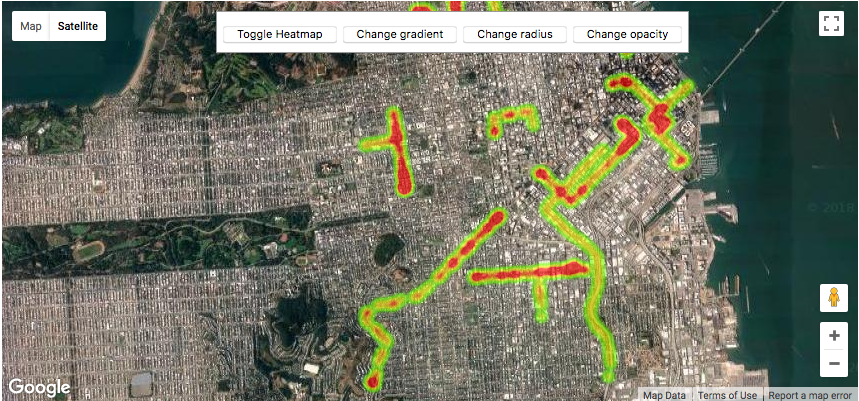
\includegraphics[width=0.7\textwidth]{googleapi_heatmap_layer}
\caption{Heatmap Layer example from the Google API website \citep{google2018heatmap}.}
\label{heatmap}
\end{figure}

\cite{Devarakonda2013} successfully used this Heatmap Layer for real-time air quality monitoring. Their air quality data was stored in a Google Fusion Table, which is part of their cloud offering and acts like a database, providing seamless integration between the data and Google's visualisation tools. The air quality data is shown neatly on top of the map with the red/green colour scale representing high/low pollution respectively. From this map, hotspots can quickly be linked to specific road layout points. For example, the authors identified a hotspot at an intersection where traffic was merging. This indicates that this method is suitable for identifying troublesome areas of high pollution.

An alternative is to use a custom coloured shape overlay on a map. For example, \cite{Hoang2013hanoihexagons} used hexagons, shown in Figure \ref{hanoihexagons}. The hexagonal shapes were used instead of the more widely used rectangular shapes because of their visual advantages. Firstly, there is less map ambiguity, and secondly, hexagonal shapes are easier for human vision to interpret since, on the map, there are no distinct horizontal and vertical lines, to which the authors note human vision is especially sensitive to. 

\begin{figure}[!tb]
\centering
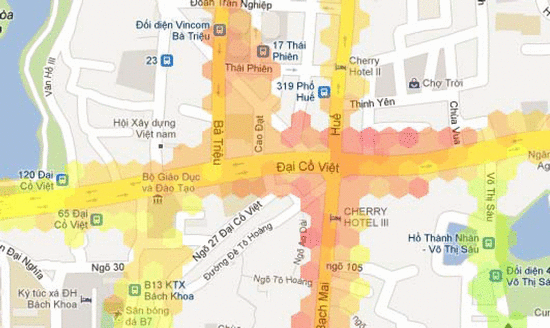
\includegraphics[width=0.7\textwidth]{hanoihexagons}
\caption{Heatmap using hexagonal shapes \citep{Hoang2013hanoihexagons}.}
\label{hanoihexagons}
\end{figure}

Another way of visualising air pollution is through the use of a grid of tiles, which is similar to the technique used by \citeauthor{Hoang2013hanoihexagons}, but uses squares instead of hexagons. The underlying map can be discarded and a graph made completely of these tiles. This is known as a raster. This was successfully used by \cite{Hasenfratz2015highresmapsTram} to create high resolution maps of pollution in Zurich. A sample of their map is shown in Figure \ref{fig:raster}.

\begin{figure}[!htb]
\centering
\includegraphics[width=0.5\textwidth]{images/raster}
\caption{High resolution raster created by \cite{Hasenfratz2015highresmapsTram}.}
\label{fig:raster}
\end{figure}

\section{Health-optimal route planning}

One potential application of air quality data is in alternative route planning for the public that takes into account pollution levels on different streets. Typically, route planning has focused on finding the shortest route from an origin to a destination. However, recent developments have begun to incorporate other factors. In particular, air pollution has begun to be incorporated into route planning \citep{sharker2014exposureroutes, Hasenfratz2015highresmapsTram}.

\cite{Hasenfratz2015highresmapsTram} use trams in Zurich to generate high-resolution pollution maps, which are then used to identify pollution levels on every street in a given section of the city. They use the product of the pollution level and the length of the road segment to add weights to the roads. These weights are then used by the A* search algorithm to generate lowest air pollution exposure routes. The authors find that travelling along these alternative routes leads to a 7.1\% reduction in air pollution exposure for a 6.4\% increase in route length.

\cite{sharker2014exposureroutes} conducted a similar US-based study. The authors overcame the issue of low spatial resolution data by assigning weights to roads from sparse fixed monitoring stations using two different interpolation methods: (i) Inverse Distance Weighting (IDW), and (ii) Kriging. The authors used Dijkstra's algorithm for their search algorithm. Overall, they found an 11.8\% reduction in pollution exposure at a cost of an 8.6\% increase in route distance by using the alternative routes. They also looked at temporal changes in road weightings and found them to be higher during the daytime, especially around midday. Interestingly, they found travel time to be lower on average for lower exposure routes. This was attributed to travelling more along highways, which have a higher speed limit, in order to avoid congested road segments. Whilst the author did not focus on a specific vehicle type, this finding may not relate well to cyclists because the larger and faster roads are often more dangerous, which may deter cyclists from cycling along them. Furthermore, cyclists cannot cycle along motorways in the UK. 

\section{Data quality monitoring}

Outlier/anomaly detection is important in the process of data cleaning. An outlier is defined as a value that is statistically different from other similar observations. Since the low-cost sensors are known to have accuracy issues (see Section \ref{lowcostsensors}), it is particularly relevant to data from low-cost sensors. To ensure the quality of the data, these will need to be identified and then corrected or removed from the data.

A simple method of identifying outliers is checking whether an observation falls within a certain confidence internal or not. A recent application of this to air quality monitoring comes from \cite{vanZoest2018outlierdetection}. They first divided up NO\textsubscript{2} data into spatio-temporal classes because different classes may have different characteristics that affect whether a measurement is an outlier or not. For each class, a threshold was calculated, from which outliers could be detected.  However, care must be taken to ensure that an extremely high pollution measurement is an error and not caused by an event, such as extreme traffic. The authors also noted that future research is needed to apply this method to real-time outlier detection.

Another method of identifying these erroneous measurements is through the use of automatic outlier detection. This term applies to a wide range of techniques, but one such technique is k-nearest neighbours in which the distance between a data point and the $k$th nearest data point is calculated. The greater this distance, the more likely the observation is an outlier. A different technique is clustering in which data points are grouped into sets of similar data points. Observations deemed not to be in any cluster are classified as outliers.

There appears to be a lack of papers applying outlier detection to air quality monitoring, particularly for more advanced outlier detection methods. This could be a potentially new application that needs to be researched further.



\section{Summary}

Air pollution is a major problem around the world, with serious negative health consequences. As a result, the \cite{WHO2002ambientmonitoring} have identified a clear need for monitoring air pollution and governments have put great emphasis on identifying which pollutants are most worth targeting. However, to effectively monitor air pollution, they need a low-cost, ubiquitous system of monitoring devices, but current government monitoring systems have a significant cost barrier. Previous work has attempted to provide a cheaper and more portable method of measuring air quality than using industrial-grade sensors, with numerous studies using a Raspberry Pi as the computer upon which the sensing platform is based. These studies have implemented various vehicles, including bicycles, tricyles, cars and trams. This mobility advantage over fixed monitoring systems has led to an improvement in the spatial resolution of the measurements. In addition, the increased availability of low-cost sensors has enabled the cost reduction, although at the cost of lower accuracy. As a consequence, methods such as machine learning have been developed in order to improve their accuracy. This air quality data can then be presented to the public and be used to inform public health decisions, such as health-optimal transport routing and where to build bike paths.

This literature review has identified a number of gaps in the literature that this project will attempt to address. These are as follows:

\begin{enumerate}
\item Creating an air quality monitoring device that measures a number of the pollutants set out by the UK and EU's air quality guidelines
\item Assessing the capabilities of a Raspberry Pi for air quality monitoring purposes
\item Whether using a bicycle is a suitable vehicle for air quality monitoring
\item Whether a number of sensing capabilities can be incorporated into one, sufficiently small device
%\item Whether calibration of air quality sensors in near real-time is feasible/possible
\item Assessing the air flow needs of bicycle-based sensors
\item Applying outlier detection methods to air quality data %, especially in near real-time
\item Mapping air pollution accurately from low-resolution data by using the techniques detailed in Section \ref{estimationtechniques}
\item Whether air pollution data can be incorporated into route planning for public benefit
\end{enumerate}

%%%%%%%%%%%%%%%%%%%%%%%%%%%%%%%%%%%%%%%%%%%%%%%%%%%%%%%%%%%%
%%%%%%%%					AIR QUALITY MONITORING DEVICE				       %%%%%%%%
%%%%%%%%%%%%%%%%%%%%%%%%%%%%%%%%%%%%%%%%%%%%%%%%%%%%%%%%%%%%


\chapter{System design and implementation} \label{chap: system_design}

In order to answer our research questions detailed at the end of Chapter \ref{chap: related_work}, we developed an air quality monitoring device that attaches to a bicycle. The device is based upon a Raspberry Pi computer and includes a variety of different sensors. These are as follows: temperature and humidity sensor, particulate (PM) sensor, ozone (O\textsubscript{3}) sensor and a general air quality sensor that is sensitive to a variety of gases that includes nitrogen oxides (NO\textsubscript{x}) and carbon monoxide (CO). It also has a GPS module attached that provides geo-location information. The device sends the collected data to a database, which is then processed and displayed in a web application. 

In this chapter, we describe the design and implementation of the air quality monitoring device, providing our rationale for both the physical construction and the software design.

\section{Physical device}

This section details how the device is constructed. Images of the final device are shown in Figure \ref{device}, which shows both the outside and inside of the device.

\begin{figure}[!htb]
\centering
\begin{subfigure}{.5\textwidth}
  \centering
  \includegraphics[width=1\linewidth]{images/device_outside}
  \caption{Outside}
  \label{fig:outside}
\end{subfigure}%
\begin{subfigure}{.5\textwidth}
  \centering
  \includegraphics[width=1\linewidth]{images/device_inside}
  \caption{Inside}
  \label{fig:inside}
\end{subfigure}
\caption[Finished device.]{The finished device. (a) shows the outside view \{1: GPS, 2: particulate sensor, 3: general air quality sensor, 4: ozone sensor, 5: temperature and humidity sensor\}. (b) shows inside the case.}
\label{device}
\end{figure}

% Label image to show which parts are which.


\subsection{Technical details}

The core of the sensing device is a Raspberry Pi Zero W single-board computer, with a 1 GHz CPU running the Raspbian Stretch, Linux-based, operating system\footnote{Link to download: \href{https://www.raspberrypi.org/downloads/raspbian/}{https://www.raspberrypi.org/downloads/raspbian/}}. The sensing capabilities come from a Shinyei PPD42 particulate sensor, a MikroElektronika Ozone 2 Click, a MikroElektronika Air Quality Click and a DHT22 temperature and humidity sensor. The MikroElektronika sensors are connected to the RPi using a MikroElektronika Pi 3 Click Shield. A GlobalSat BU-353S4 USB GPS receiver supplies the precise geospatial information for geo-tagging the air quality measurements. The built-in WiFi of the RPi is used to connect to a WiFi hotspot in order to upload the measurements to a MySQL database (version 5.7.16 Community Server) via a PHP script. An Android mobile phone running Android 6.0.1 is used to provide the WiFi hotspot whilst cycling. The program running on the RPi is written in the Python programming language and can be found in Appendix XXX. The power for the device is supplied via a 10000mAh external battery pack, with a 5V 2.4A output. The web application is written in R and uses R Shiny to generate the interface.

\nomenclature{GPS}{Global positioning system}

\subsection{Raspberry Pi}

The original plan uses a Raspberry Pi Zero W as the base computer, but in testing an overheating issue was encountered, rendering an RPi completely useless. The device's CPU was running extremely hot, which is potentially a side-effect of the device containing a large number of sensors. RPis do not come with heat-sinks, but these could be included in future designs. To fix the issue of overheating, we switched to a Raspberry Pi 2. The Raspberry Pi 3 was also tested as an alternative, but the Serial Peripheral Interface (SPI) setup is different and so the software did not run correctly (see Section \ref{rpi_software} for SPI details). The device does not need the additional computing power, so the Raspberry Pi 2 is deemed to be satisfactory.
% Mention issue of RPi 2 also breaking.
% Tense??

\subsection{GPIO}

GPIO stands for General Purpose Input/Output and provides a standardised interface for the RPi to a variety of other devices. The device's RPi has 40 GPIO pins, of which 17 are used. The active pins are detailed in Table \ref{gpio}. Given the number of sensors attached to the device, it is difficult to connect them all to the GPIO pins of the RPi (at a minimum there are power, ground and signal wires). To overcome this, a GPIO expander is used, with care taken to ensure that GPIO pins are only used for a single signal (issues arise if multiple signals are sent on the same pin). 

\begin{table}[!tb]
  \centering
  \small
  \caption{GPIO pin layout and usage for the 40 GPIO pins on the Raspberry Pi. Of these 40, 17 are directly used by the sensors in the device.}
  \label{gpio}
  \begin{tabular}{ l l l }
  \toprule
  Pin & BCM \# & Usage \\ \midrule
  1 & 3v3 power & DHT22 power  \\
  3 & BCM 2 &  \\
  5 & BCM 3 &  \\
  7 & BCM 4 &  \\
  9 & Ground & DHT22 ground  \\
  11 & BCM 17 &  \\
  13 & BCM 27 &  \\
  15 & BCM 22 & DHT22 signal  \\
  17 & 3v3 power &  \\
  19 & BCM 10 & MQ131 MOSI \\
  21 & BCM 9 & MQ131 MISO \\
  23 & BCM 11 & MQ131 SCLK \\
  25 & Ground &  \\
  27 & BCM 0 &  \\
  29 & BCM 5 &  \\
  31 & BCM 6 &  \\
  33 & BCM 13 &  \\
  35 & BCM 19 & MQ135 MISO \\
  37 & BCM 26 &  \\
  39 & Ground &  \\ \bottomrule
  \end{tabular}
  \hspace{0.5em}
  \begin{tabular}{ l l l }
  \toprule
  Pin & BCM \# & Usage \\ \midrule
  2 & 5V power & Shinyei power \\
  4 & 5V power & MQ135/131 power \\
  6 & Ground & Shinyei ground  \\
  8 & BCM 14 &  \\
  10 & BCM 15 &  \\
  12 & BCM 18 &  \\
  14 & Ground &  \\
  16 & BCM 23 & Shinyei signal \\
  18 & BCM 24 & \\
  20 & Ground & LED ground \\
  22 & BCM 25 & LED signal \\
  24 & BCM 8 & MQ131 signal \\
  26 & BCM 7 &  \\
  28 & BCM 1 &  \\
  30 & Ground &  \\
  32 & BCM 12 &  \\
  34 & Ground &  \\
  36 & BCM 16 & MQ135 signal \\
  38 & BCM 20 & MQ135 MOSI \\
  40 & BCM 21 & MQ135 SCLK \\ \bottomrule
  \end{tabular}
\end{table}

\nomenclature{GPIO}{General Purpose In/Out}


\subsection{Particulate sensor}

A number of different low-cost particulate sensors are considered for this project, based upon previous research. These are detailed in Table \ref{particulatesensors}. \cite{garnier2017mythorreality} evaluated the Sharp GP2Y and HK-A5 particulate sensors, finding that both of these sensors had low to zero correlation with an industry-grade DustTrak 8533 particulate sensor, despite controlling for external factors. \cite{thorpe2017RPimesh} also evaluated these sensors, as well as the Shinyei PPD42 sensor. The HK-A5 sensor was found to have no response to changes in particulate concentration in preliminary testing and was subsequently excluded from the author's investigation. The author, unfortunately, could not provide much evaluation of the Sharp GP2Y sensor due to software bugs and damaged sensors. As a result, Thorpe focused on the Shinyei PPD42 sensor and found it to track changes in particulate concentration reliably, with a substantial accuracy improvement through the use of polynomial fitting or a single feature multi-layer perceptron. Therefore, the Shinyei particulate sensor is a sensible choice for use in this project.
%% NN?

\begin{table}[!tbp]
  \centering
  \caption{Comparison of different particulate sensors considered. All of these sensors use a light-scattering technique for detecting particles. The Shinyei PPD42 sensor is the cheapest, with joint-smallest minimum particle detection size.}
  \label{particulatesensors}
  \begin{tabular}{ l l l l}
  \toprule
  Sensor & Sensor type & Minimum PM size & Cost (\textsterling) \\ \midrule
  Shinyei PPD42NS & Light scattering & PM\textsubscript{1} & 7.75 \\
  Sharp GP2Y & Light scattering & PM\textsubscript{10} & 9.46 \\
  HK-A5 & Light scattering & PM\textsubscript{1} & 37.70 \\ \bottomrule
  \end{tabular}
\end{table}

The chosen Shinyei PPD42NS sensor has two output lines, named P1 and P2. P1 is used to measure particles between $1\mu m$ and $10\mu m$, whereas the P2 output is used to measure particles between $2.5\mu m$ and $10\mu m$. In testing, we rarely registered a signal from P2 that differed from P1, which would indicate that the sensor only detects particles with diameter above $2.5\mu m$. This implies the output from the sensor is classified as PM10. This agrees with the findings of \cite{thorpe2017RPimesh}, who found that the sensor responded very poorly to smoke which has an average particle size of between 1 and 2$\mu m$.

The sensitivity of this sensor is a clear drawback if accurate measurements of PM2.5 are needed. However, we are more interested in creating a working air quality monitoring device and testing the effectiveness of a bicycle-based device, meaning a lower accuracy can be afforded. Moreover, PM10 is still a governmentally monitored pollutant in the UK (see Table \ref{airqualityguidelines}) and provides a solid measure of air quality. Nonetheless, it is still worth noting this issue for future developments.

\subsection{Ozone sensor}

For the gas sensors, we opt for using MikroElektronika's click-board technology, which provides a homogeneous platform that a variety of sensors can be plugged directly into without the need for soldering. This dictates our choice of ozone sensor because MikroElektronika only have one option available -- the `Ozone 2 Click'. This click-board uses an MQ131 sensor on the circuit board, which has a tin dioxide sensing layer that reduces in conductivity in clean air. It can detect ozone concentrations between 10 and 1000 parts-per-billion (ppb).

One of the main reasons for choosing to use MikroElektronika's click-board technology is the modular nature of the sensors, which all use the same 16-pin design. This means we can easily change sensors quickly to suit our requirements and re-purpose the air quality monitoring device at short notice, therefore avoiding soldering of circuit boards.

The MQ131 ozone sensor has been used in air quality projects previously, including in a unmanned aerial vehicle (UAV) air quality monitoring device \citep{alvear2017uav} and indoor monitoring \citep{Abraham2014costeffindoor}.

\subsection{NO\textsubscript{x} sensor}

For an NO\textsubscript{x} sensor, we chose the MikroElektronika `Air Quality Click'. This uses an MQ135 sensor and is marketed as being sensitive to NO\textsubscript{x}. However, upon further analysis, one can see that NO\textsubscript{x} is not listed on the data sheet's calibration curves and the sensor is actually sensitive to a variety of different gases. Unfortunately, the company did not have any dedicated NO\textsubscript{x} sensors available to replace this with. As a result of this issue and the project's time constraints, we use it as a general air quality sensor.

Nonetheless, as previously explained, the modular nature of MikroElektronika's click-board technology means it would be easily replaceable in the future. In fact, towards the end of the project, MikroElektronika released a dedicated NO\textsubscript{2} sensor. This is worth noting for future developments of this air quality monitoring device.

A number of previous studies use the MQ135 sensor for air quality monitoring purposes. \cite{Rahman2017adaptivesensingRPi} used the MQ135 in an Internet-of-Things (IoT) based platform, whilst \cite{anderson2012noxdroid} used it on a bicycle-based air quality monitoring device. In addition, \cite{garnier2017mythorreality} tested the MQ135 and found it to be accurate for monitoring changes and trends in air quality.

\subsection{Temperature and humidity sensor}

A DHT22 temperature and humidity sensor adds climate monitoring capabilities to our device. \cite{garnier2017mythorreality} found the DHT22 to be more accurate than a BME280 sensor (another commonly used temperature and humidity sensor), despite costing less. This sensor has been used frequently elsewhere in the literature \citep{Rahman2017adaptivesensingRPi, ibrahim2015IOTenvmon, alkandari2018airqualityexperimental}. By including this sensor in the device, we are able to correct the particulate and gas sensor measurements, which are sensitive to temperature and humidity at certain levels.

\subsection{HAT}

The Mikro Pi 3 Click Shield, which holds the ozone and general air quality sensors, uses a 40-pin GPIO connector to interface with the RPi, although not all of the pins are used (see Table \ref{gpio}). Therefore, in order to attach the particulate sensor, the temperature and humidity sensor and the LED to one RPi, a solution is needed that enables other connections to the GPIO pins.

The chosen solution is a GPIO expansion board (see Figure \ref{fig: gpio_expander}), which provides 4 additional 40-pin GPIO connectors. Figure \ref{fig: two_on_one} shows how the multiple connections are made. The particulate sensor has a digital output and so can be connected directly to the GPIO pins with the use of a voltage divider made out of a $2.2k\Omega$ and $3.3k\Omega$ resistor. The temperature and humidity sensor and LED also have digital outputs, meaning they are connected directly to the GPIO pins as well. These connections to the GPIO expansion board are made more robust through the use a custom-built circuit board. A protoboard has a GPIO connector soldered to its underside, which enables it to connect to the GPIO expansion board. Single lines of GPIO pins are also soldered on, along with the relevant resistors discussed previously. Female-to-female jumper cables connect the sensors and the LED to these GPIO pins. Figure \ref{protoboard} shows the final soldered protoboard.

\begin{figure}
\centering
\begin{subfigure}[b]{0.4\textwidth}
  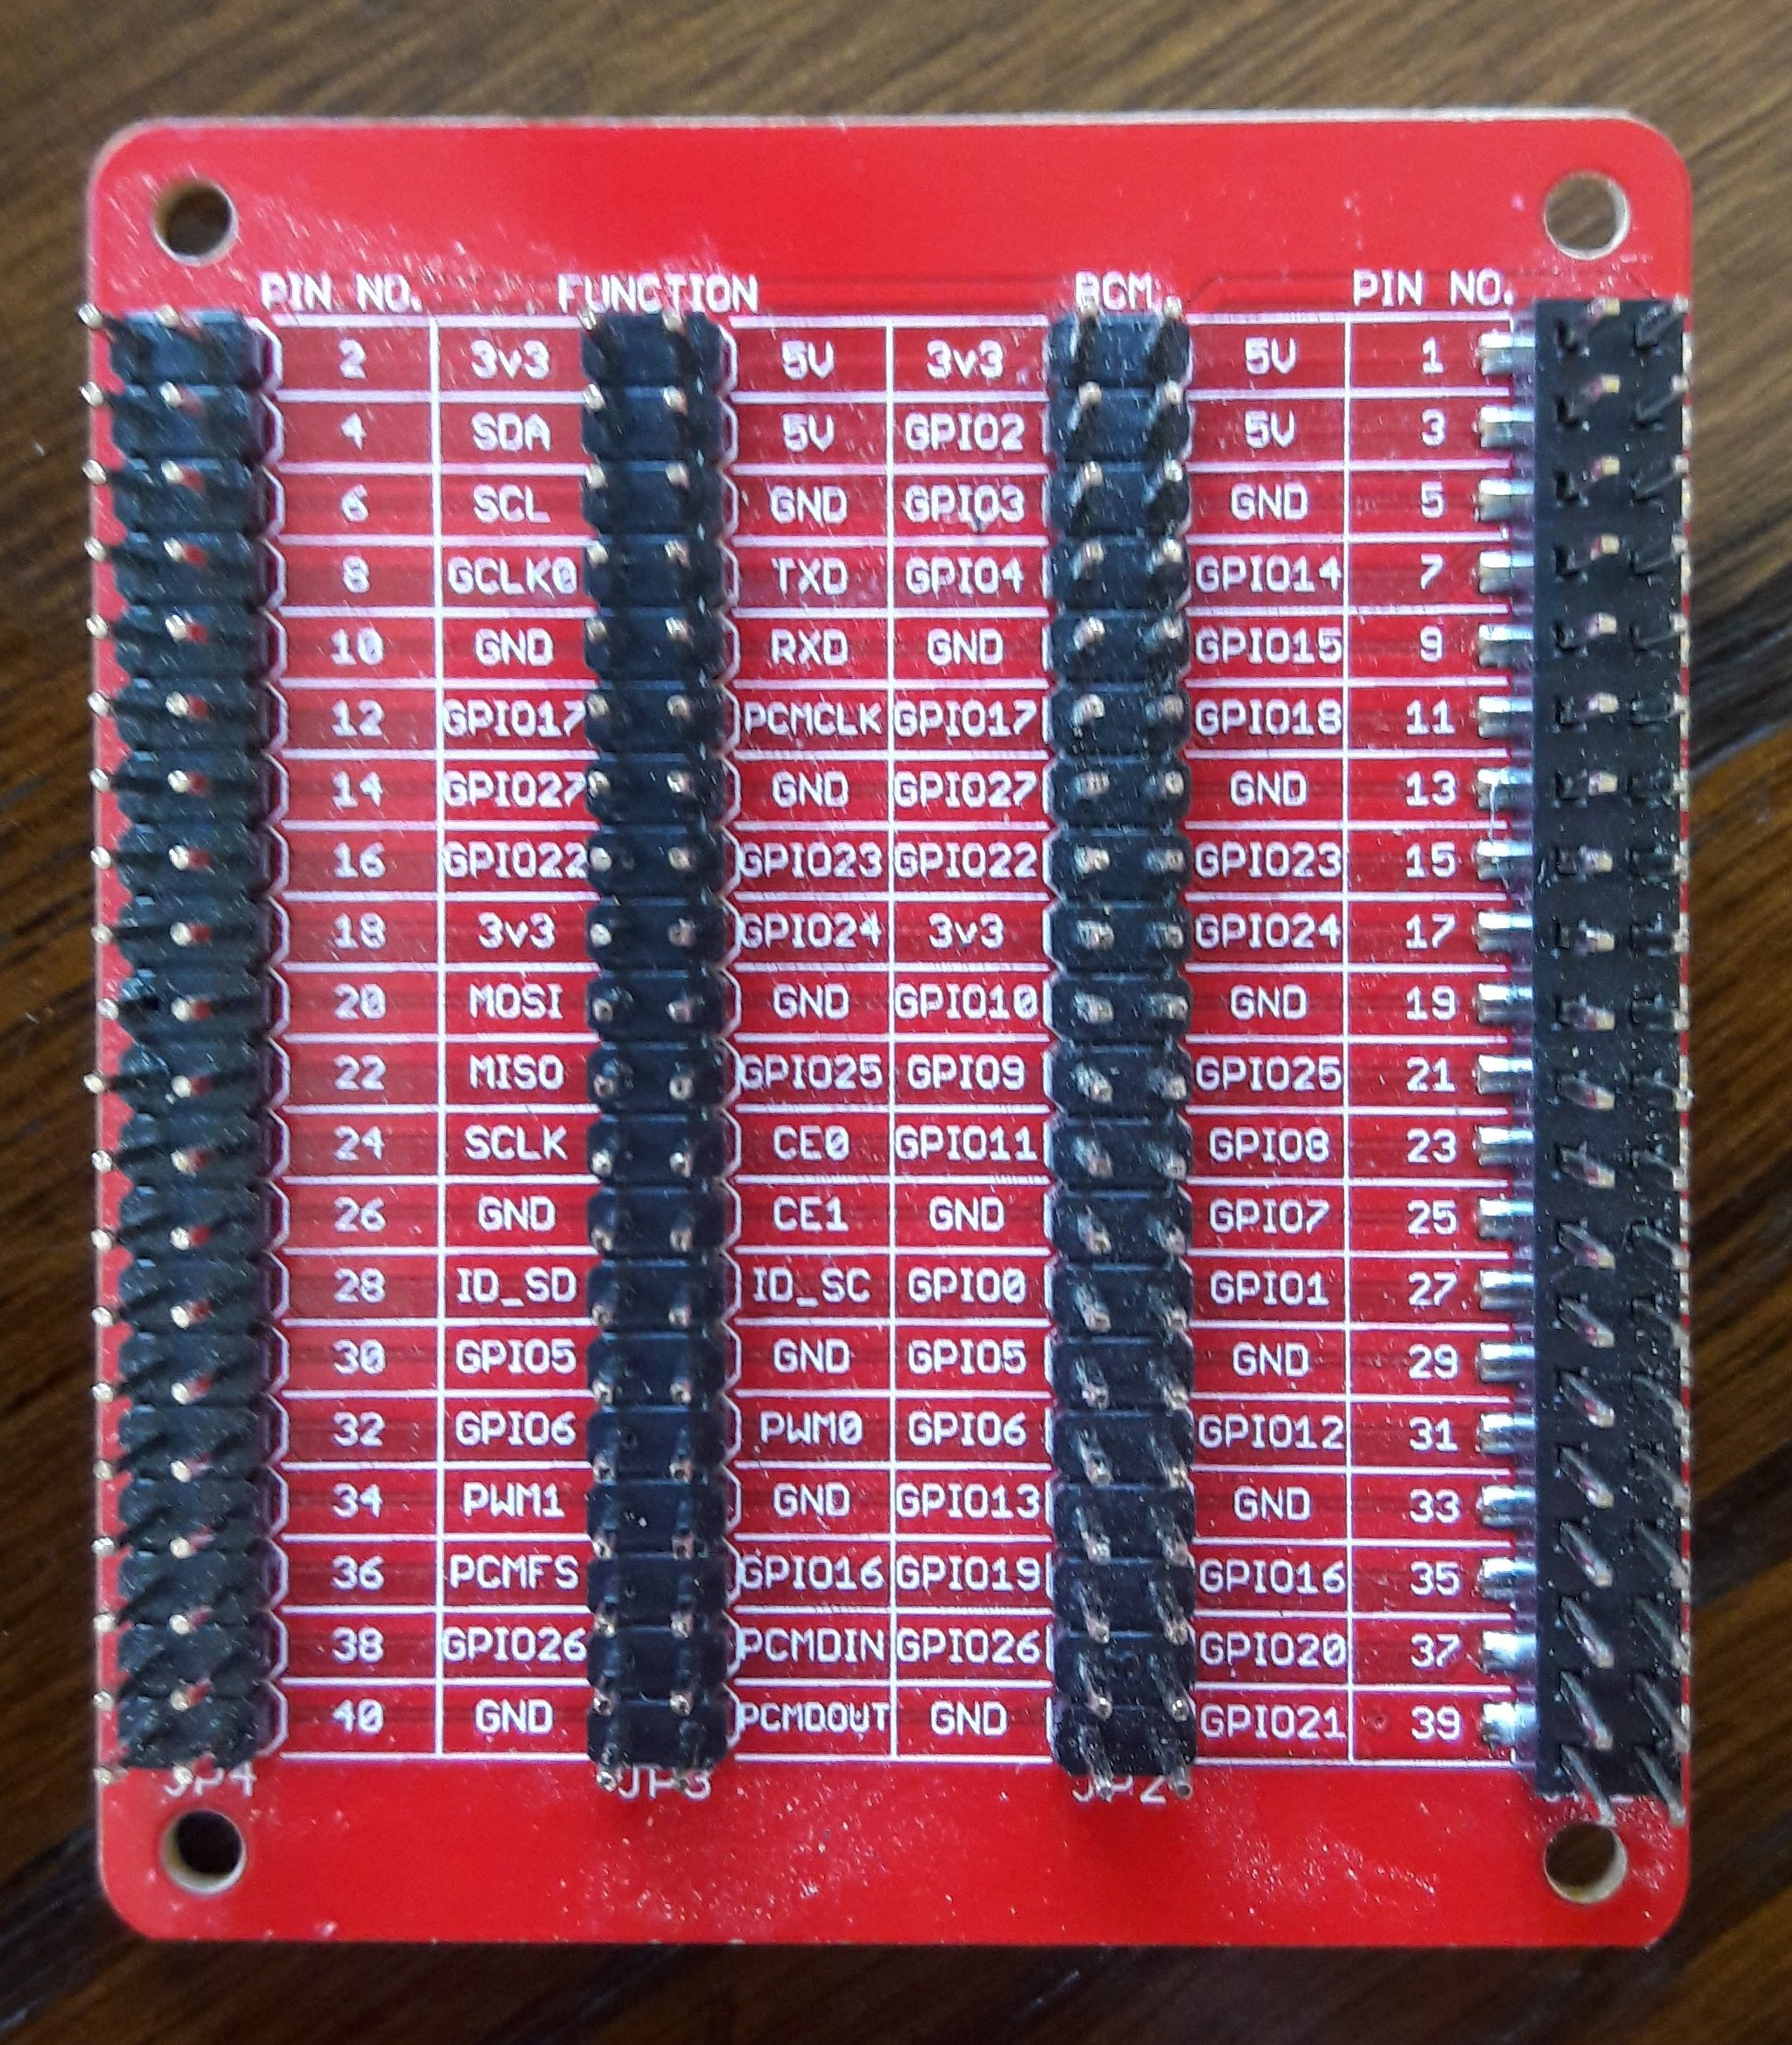
\includegraphics[width=\textwidth]{images/gpio_expander1}
  \caption{GPIO expansion board.}
  \label{fig: gpio_expander}
\end{subfigure}
\hfill
\begin{subfigure}[b]{0.5\textwidth}
  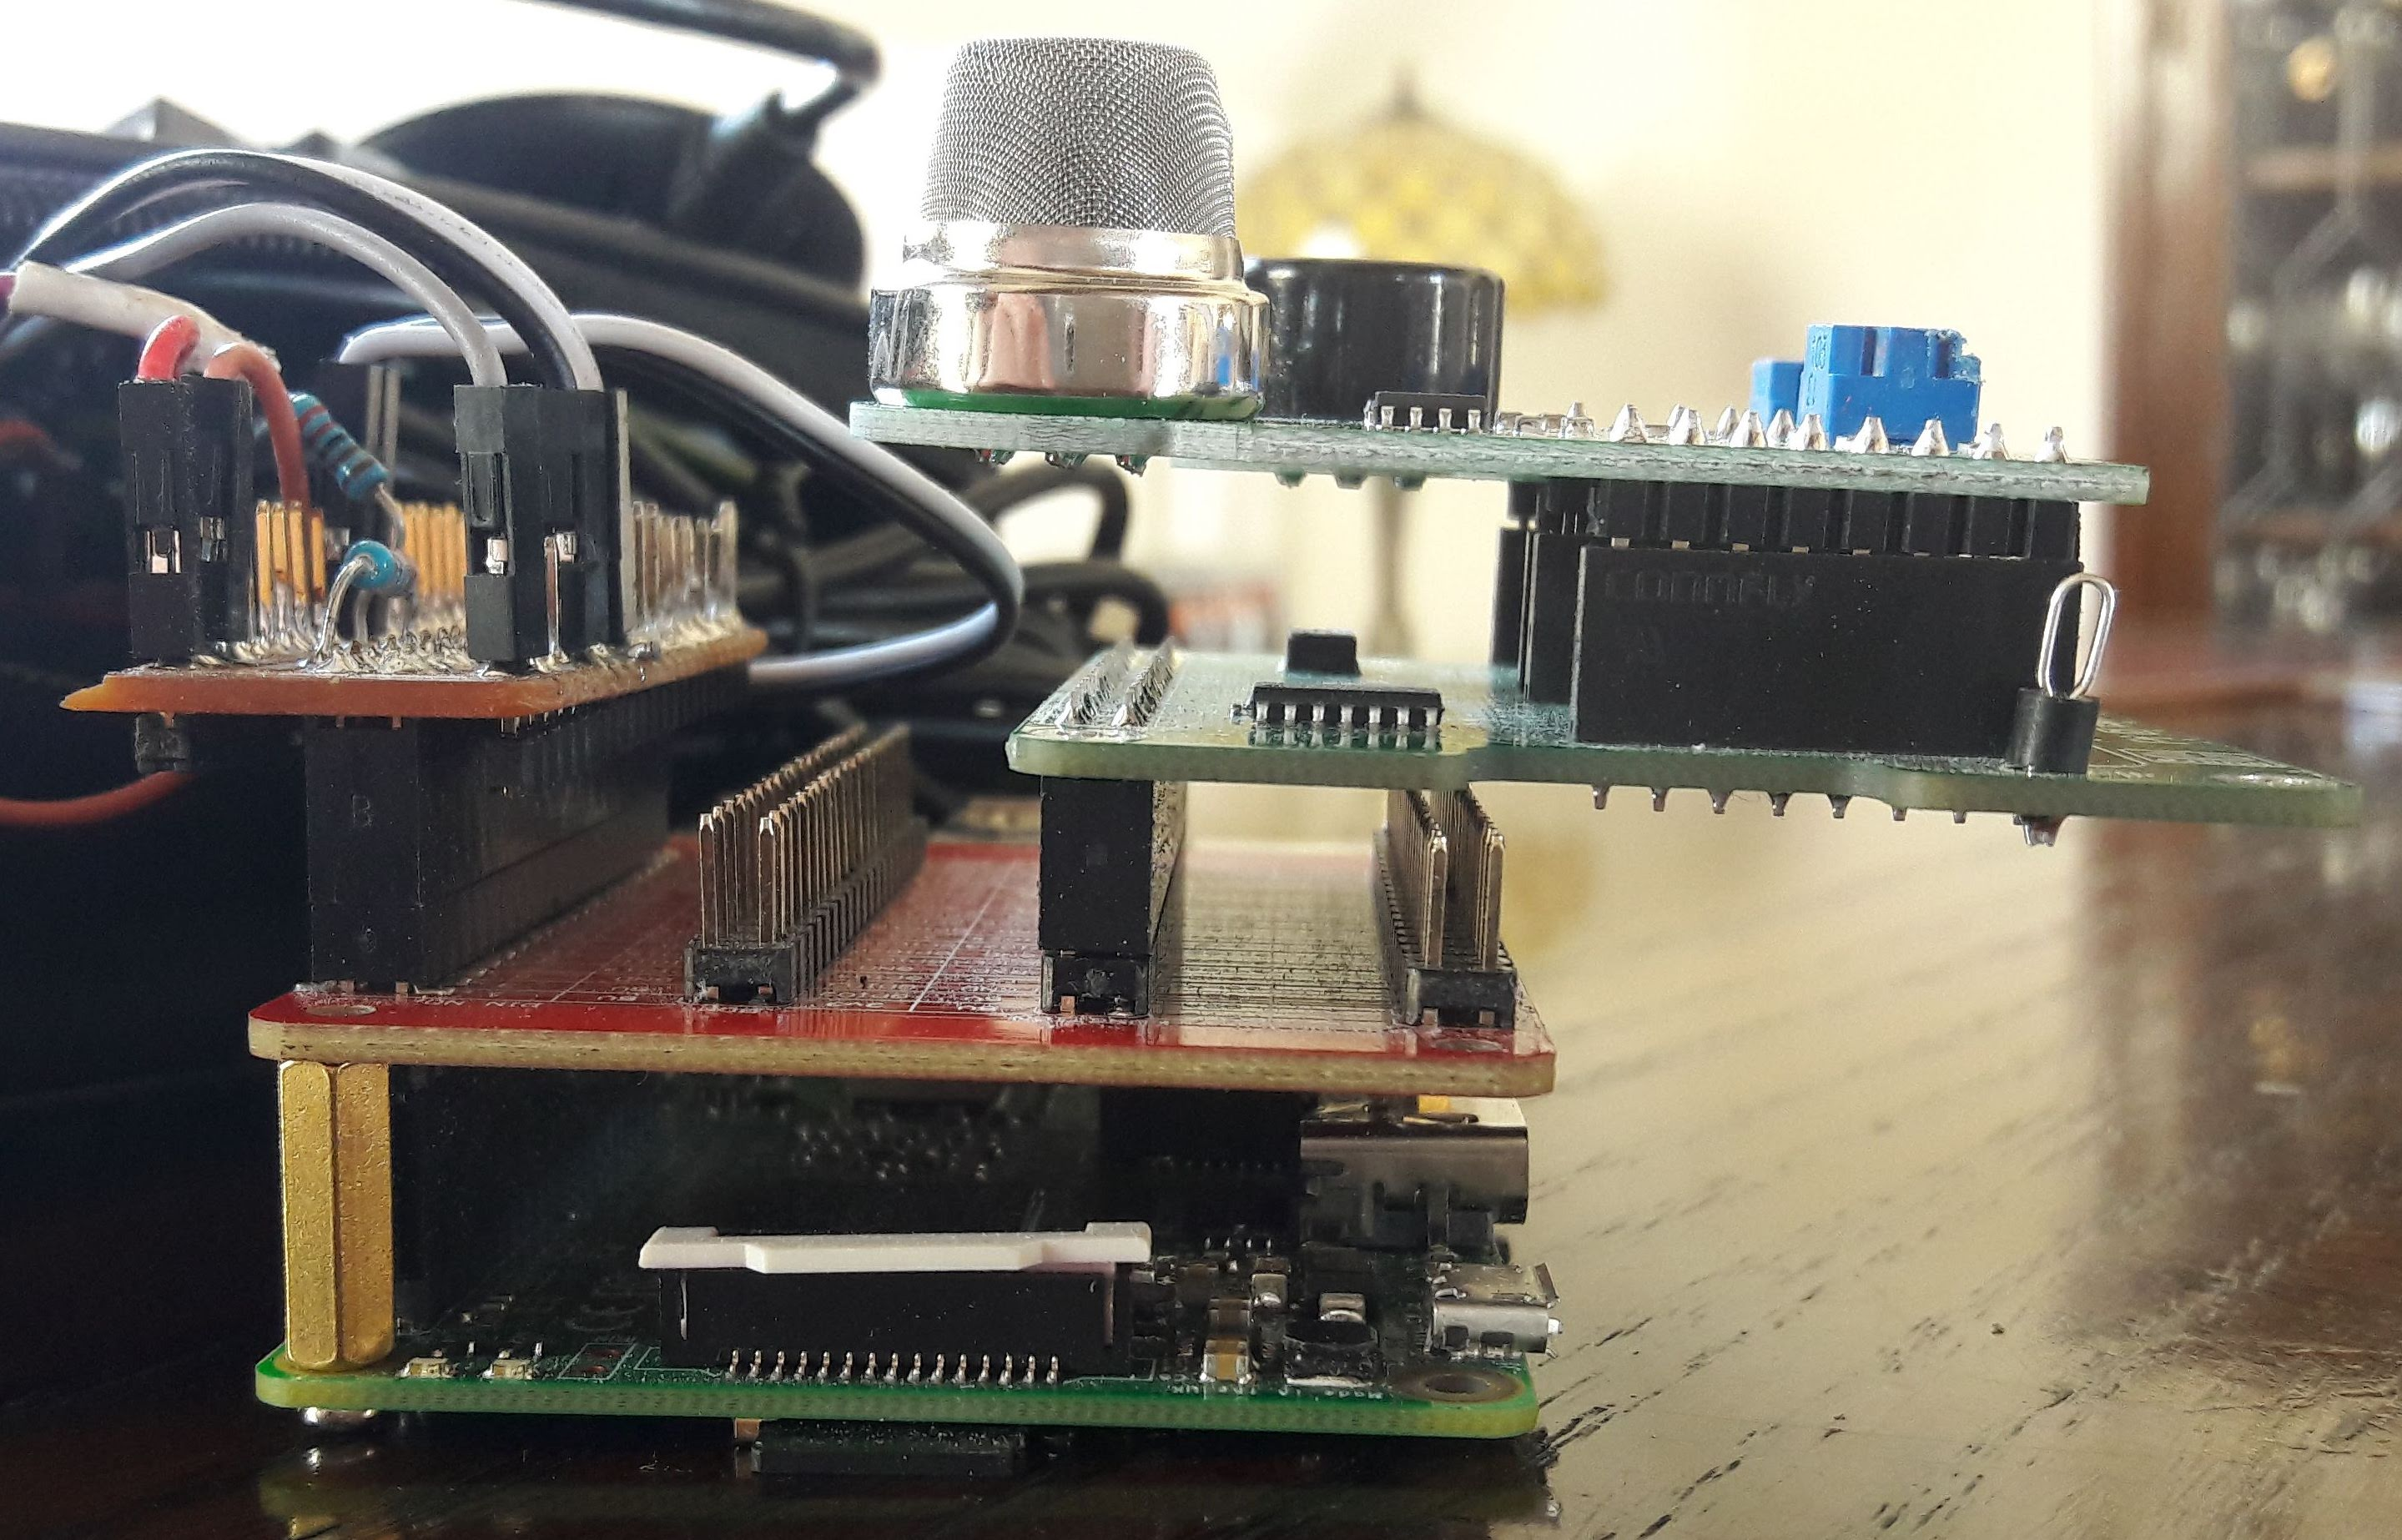
\includegraphics[width=\textwidth]{images/two_on_one}
  \caption{Two HATs connected to GPIO expansion board.}
  \label{fig: two_on_one}
\end{subfigure}
\caption[Solution to sensor attachment problem.]{Solution to sensor attachment problem. (a) The GPIO expansion board provides 4 rows of 40-pin GPIO connections. (b) 2 HATs are connected to the RPi via the expansion board, which enables our device to have increased sensing capabilities.}
\end{figure}

\begin{figure}[!tb]
\centering
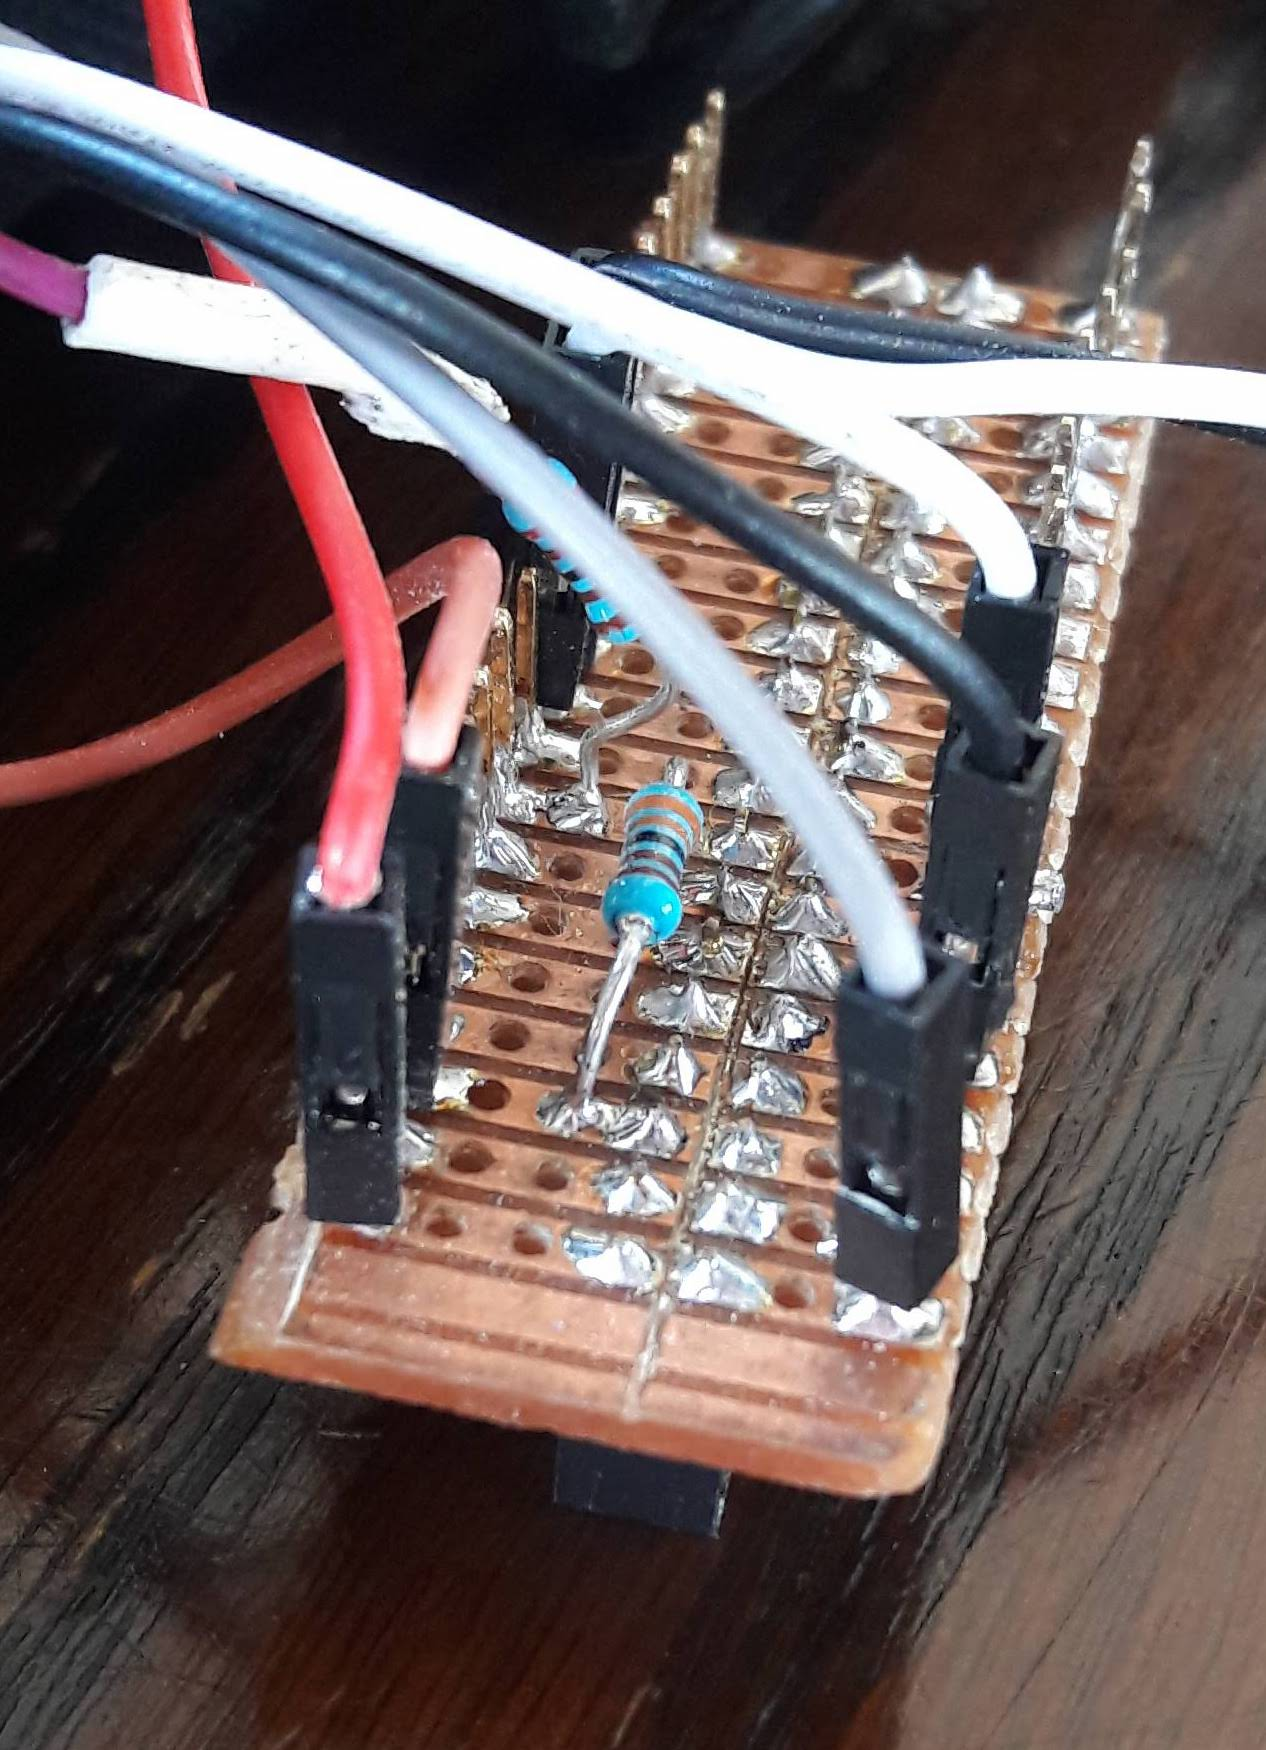
\includegraphics[width=0.4\textwidth]{images/protoboard}
\caption[Soldered protoboard.]{Soldered protoboard. This custom circuit board enables the connection of the sensors with digital outputs (Shinyei PPD42 and DHT22, as well as the LED) to the RPi.}
\label{protoboard}
\end{figure}

%For the particulate sensing, a Grove Pi+ HAT board was used to allow connection of the Shinyei PPD42 sensor to the Raspberry Pi. The HAT connects to the RPi via the GPIO pins.

%Possible to stack the HATs?

%(If not) Since Grove do not have all sensors required for this project available, a second RPi was used and connected to a Mikro Pi Click Board. This provides a similar platform to the Grove Pi+ HAT for connecting sensors, but instead uses additional GPIO pins on the Click Board to attach `click on' units with different sensing capabilities.

%%% Add in images of both boards %%%



\subsection{Power}

The power to the device is supplied by a 10000mAh lithium-ion battery. The current draw of the whole device can be measured using an ammeter, dissecting a USB cable and attaching clips to the voltage common collector (VCC) wire, commonly known as the `power' wire. This test setup is shown in Figure \ref{fig: ammeter}, with the dissected cable shown in Figure \ref{fig: usb_cable}. The ammeter reported current values between 748mA and 754mA. Therefore, the device can run for approximately 13 hours on a fully-charged battery. It must be noted that Equation \ref{eqn: time} is only an estimate because batteries typically have non-linear discharge due to factors such as temperature and age of battery.
\begin{equation} \label{eqn: time}
t = \frac{10000mAh}{750mA} = 13.\dot{3} \; hours
\end{equation}

% Try this for each part of the device and produce table?

\nomenclature{VCC}{Voltage common collector}

\begin{figure}
\centering
\begin{subfigure}[b]{0.4\textwidth}
  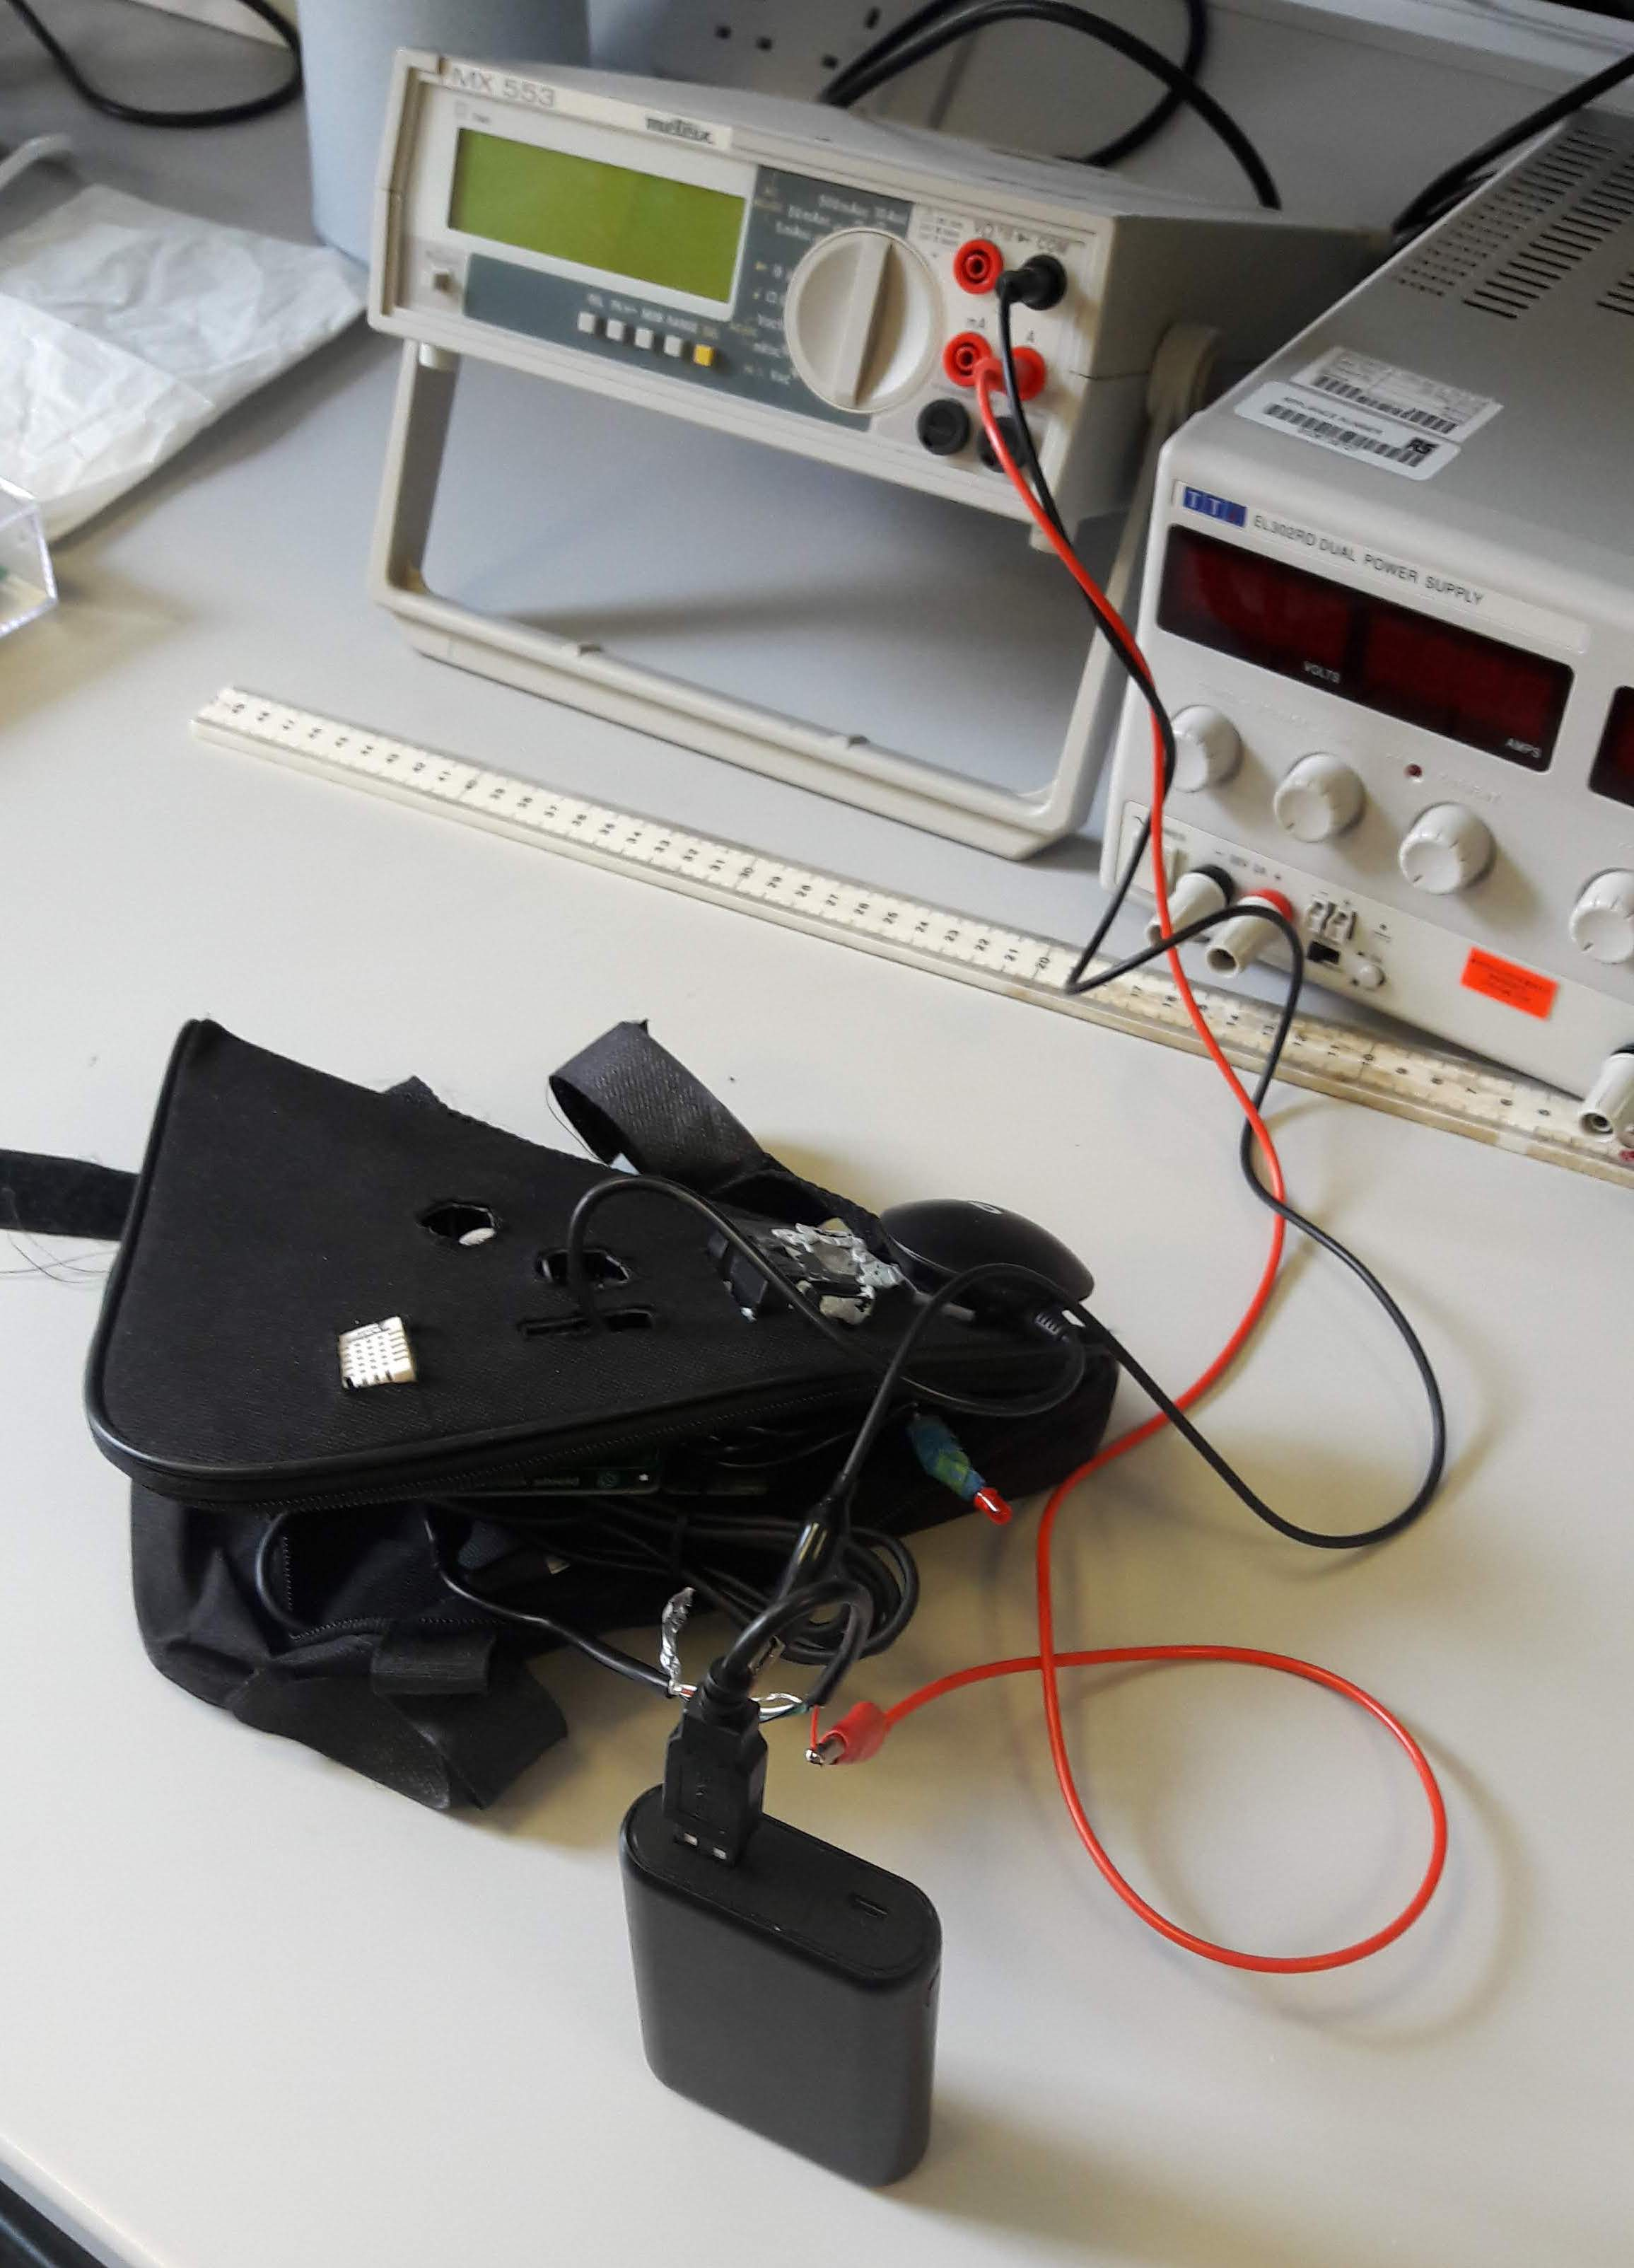
\includegraphics[width=\textwidth]{images/ammeter}
  \caption{Connection to ammeter.}
  \label{fig: ammeter}
\end{subfigure}
\hfill
\begin{subfigure}[b]{0.4\textwidth}
  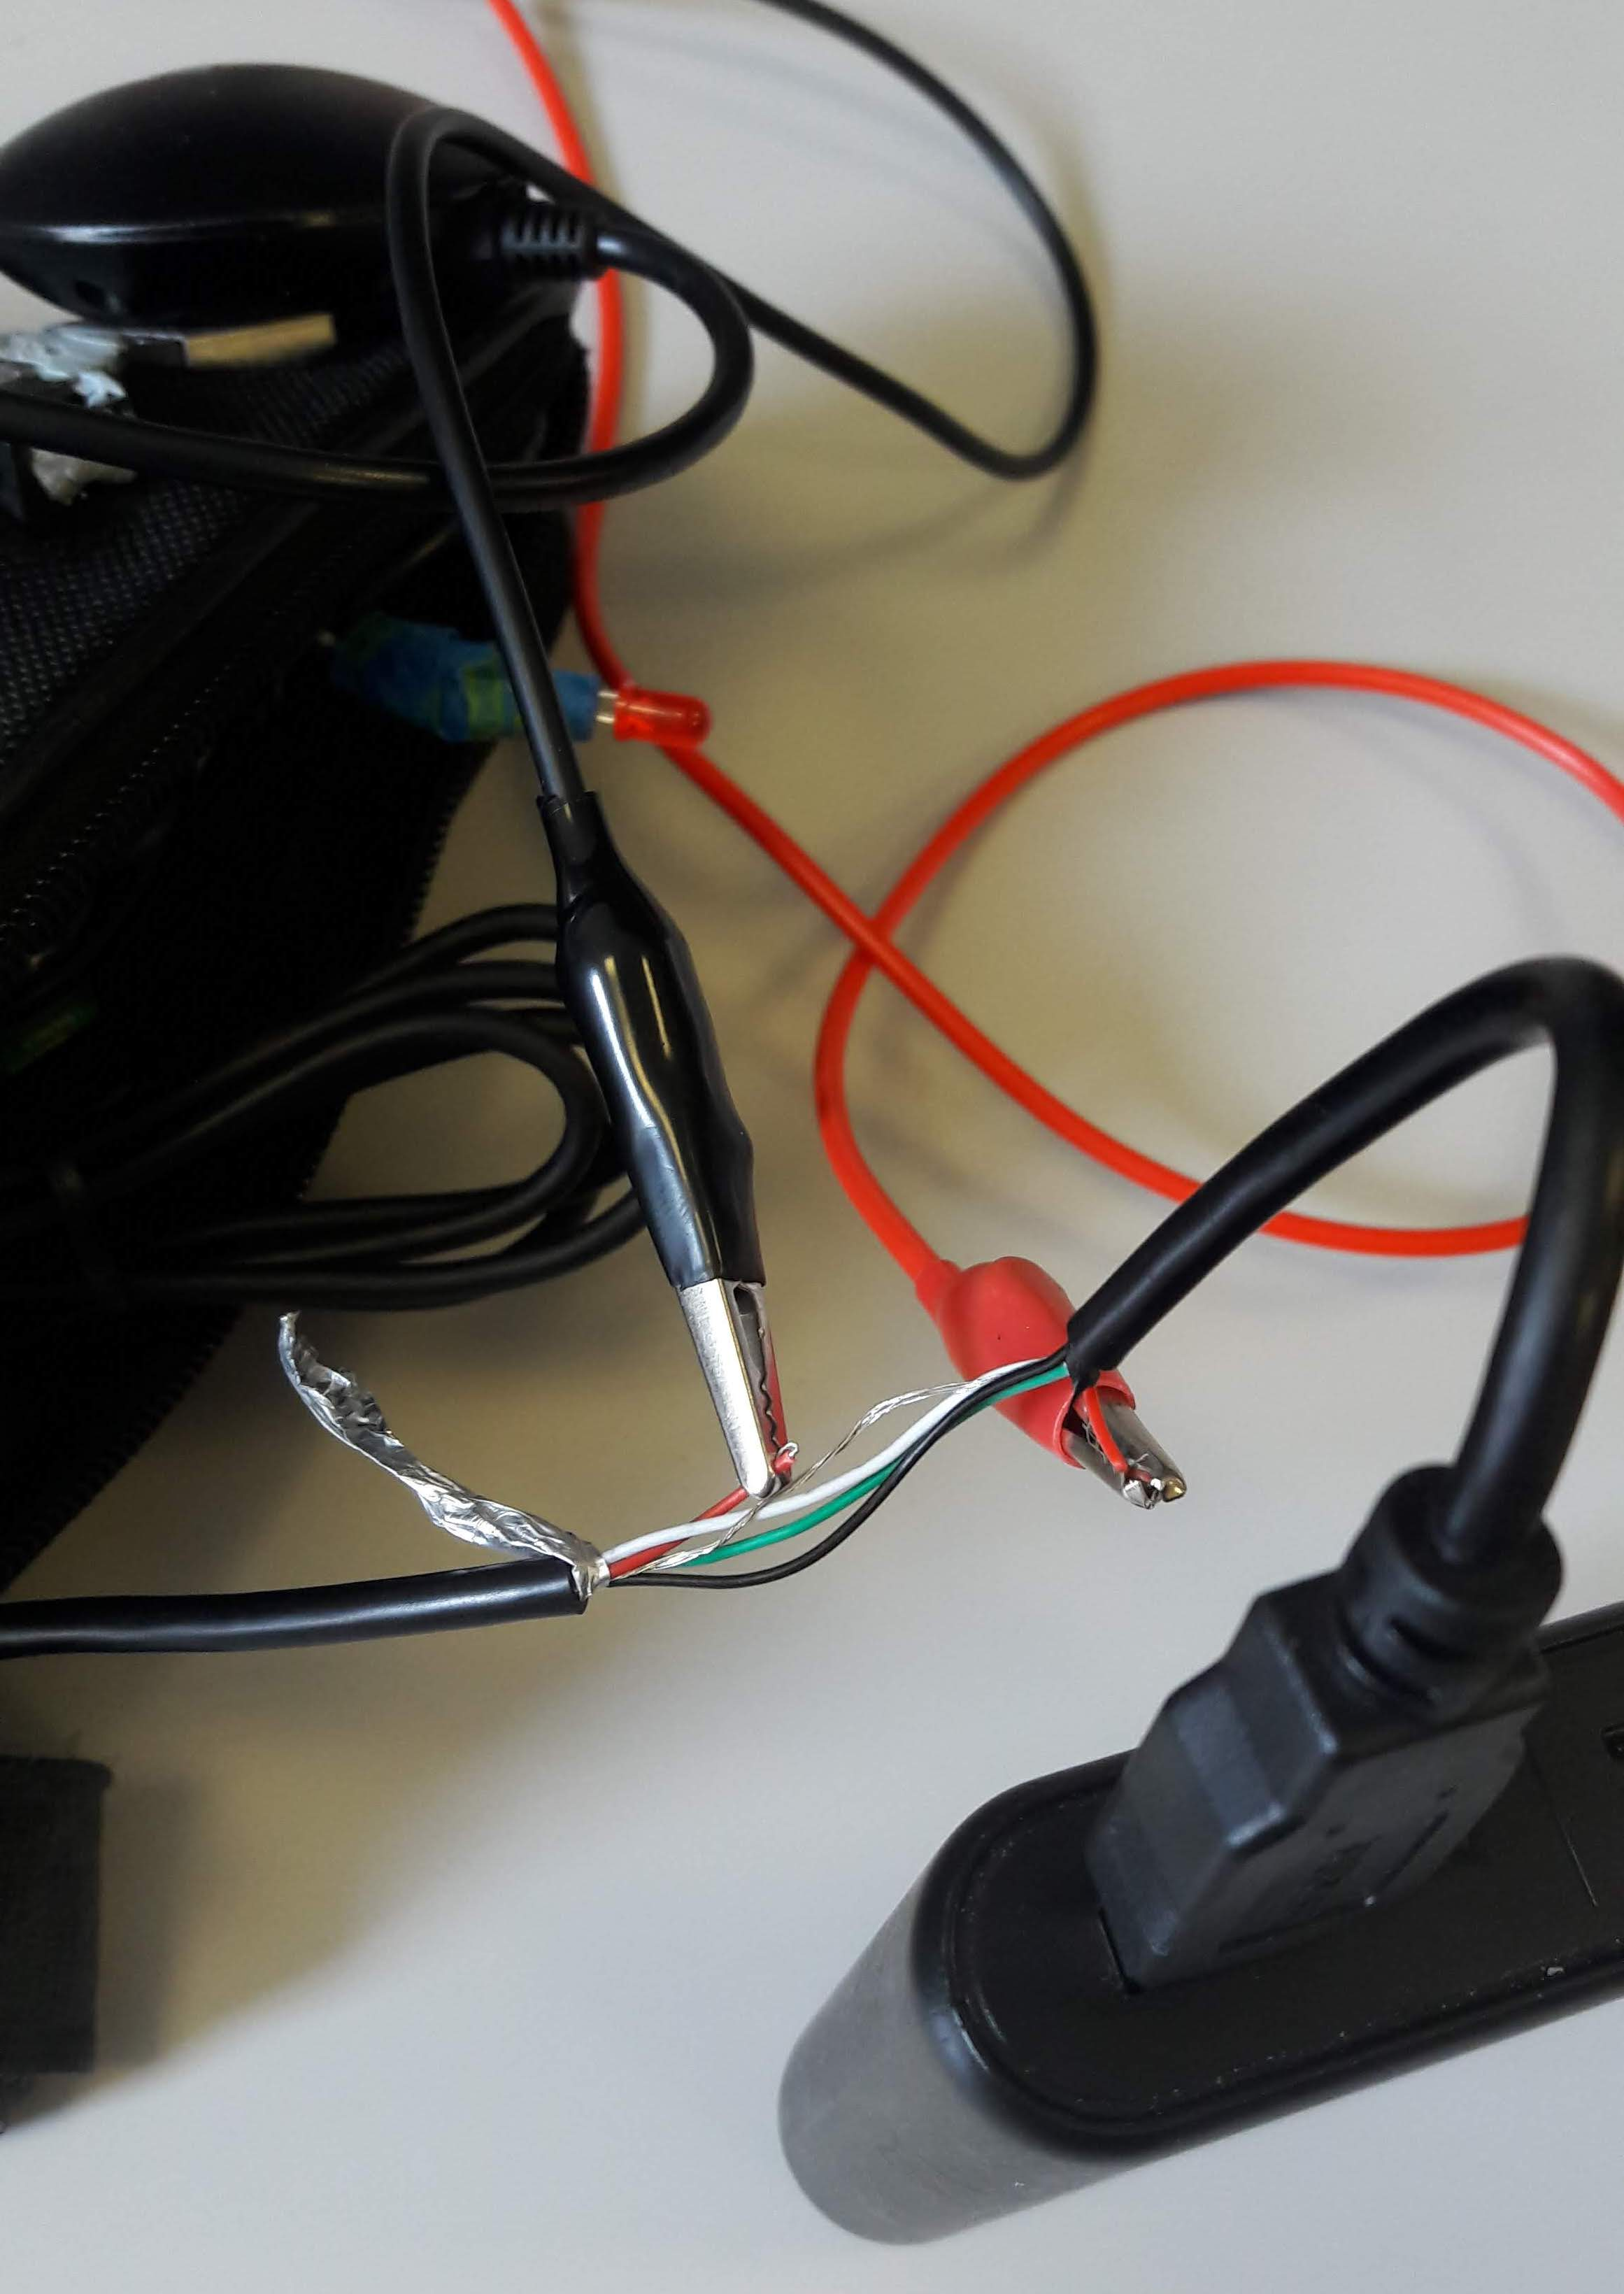
\includegraphics[width=\textwidth]{images/usb_cable}
  \caption{Dissected USB cable with VCC wire exposed.}
  \label{fig: usb_cable}
\end{subfigure}
\caption[Power consumption testing.]{Power consumption testing. (a) shows the test setup with a connection to an ammeter, and (b) shows how a USB cable is dissected to enable sampling of the current drawn.}
\end{figure}

\subsection{Case}

The case is a modified version of a triangular bag that fits to the frame of a bicycle. It has three velcro straps that secure the bag to the bicycle's frame. The inside of the bag is lined with a flexible plastic, thus helping to make the device water-resistant. There are holes cut into the side of the bag to: (a) expose the air quality sensors to the air, (b) to allow the GPS module to have a clear view of satellites in the sky, and (c) to display a system-status LED to the user.

\nomenclature{LED}{Light emitting diode}

\subsection{Cost}

One of the main aims of this project is to create a low-cost device. In total, the cost of a complete air quality monitoring device is \textsterling 152.63. A breakdown is shown in Table \ref{costs}.

\begin{table}[!tbp]
  \centering
  \caption{Cost breakdown of device. The overall cost of the device is relatively low at only \textsterling 152.63, which satisfies this project's objective of making a low-cost air quality monitoring device.}
  \label{costs}
  \begin{tabular}{ l S[table-format=3.2] }
  \toprule
  Item & {Cost (\textsterling)} \\ \midrule
  Raspberry Pi 2 Model X & 20.00  \\
  ModMyPi Triple GPIO Expansion Board & 7.99 \\
  Shinyei PPD42NS particulate sensor & 7.75 \\
  DHT22 temperature and humidity sensor & 4.99 \\
  Mikro Ozone 2 Click & 33.90 \\
  Mikro Air Quality Click & 15.91 \\
  Mikro Pi 3 Click Shield & 15.60 \\ 
  GlobalSat BU-353S3 USB GPS receiver & 30.99 \\
  10000mAh external battery pack & 15.00 \\
  Jumper cables & 0.50 \\ \midrule
  Total & 152.63 \\ \bottomrule
  \end{tabular}
\end{table}

Given the device uses the mobile phone's cellular network to upload the measurements, it is also worth noting the data plan cost. The device generates 542 bytes/minute of data on average when sampling every 10 seconds. With an average running time each day of 2 hours, the device will use around 2 MB of data per month. Assuming a 5GB data plan per month costs \textsterling 10, the data consumption of this device costs \textsterling 0.004 per month. This is negligible. 

\newpage
\section{Software}

The software for this air quality monitoring device covers a number of different areas.
\begin{enumerate}
\item Software that runs on the Raspberry Pi to collect and send the sensor data (Section \ref{rpi_software})
\item Server-side software that receives the data and inserts it into a database (Section \ref{server_software})
\item Web application that displays the data to the public (Section \ref{web_application})
\end{enumerate}

\begin{figure}[!tb]
\centering
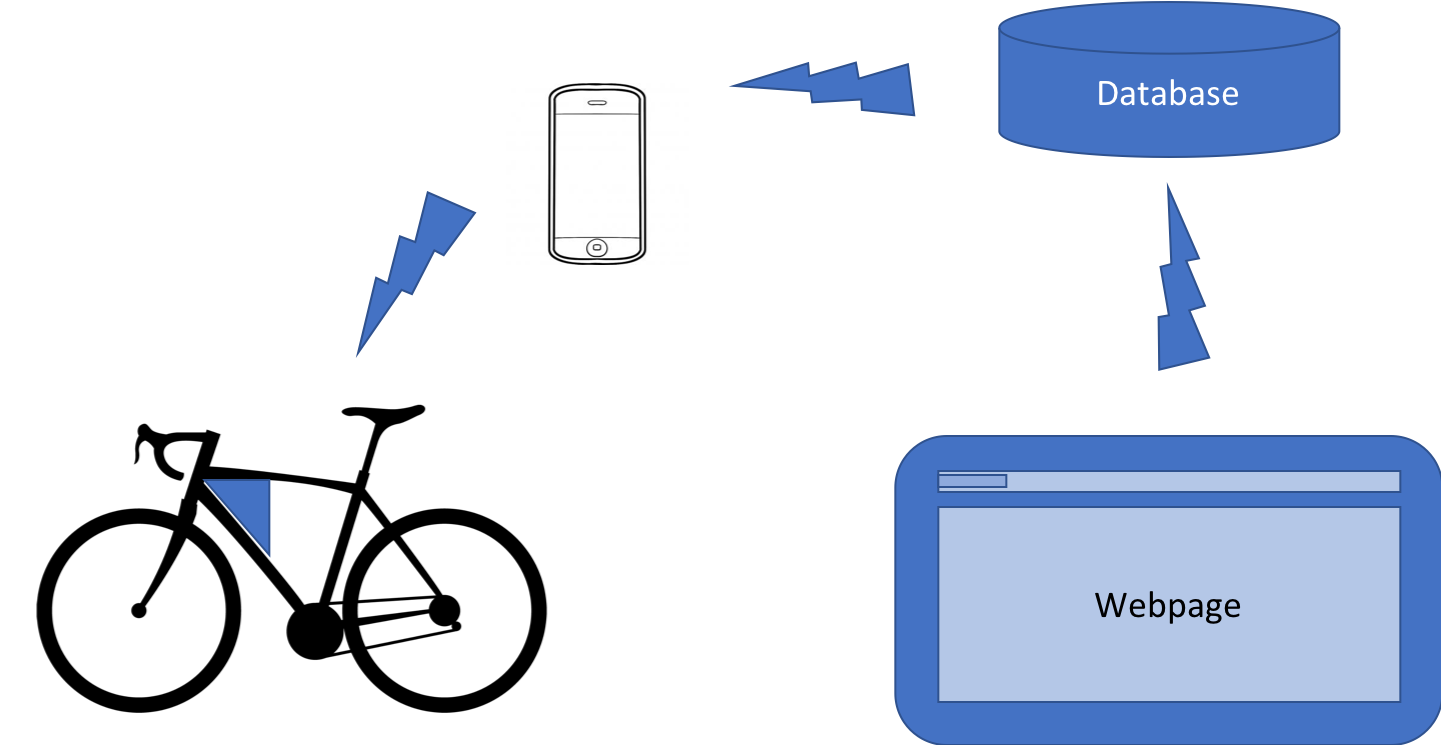
\includegraphics[width=0.9\textwidth]{images/design}
\caption[Data flow.]{Data flow. The device attached to the bicycle sends data to a database using the phone's internet connection, which is then displayed on a webpage.}
\label{design}
% Update drawing
\end{figure}

\subsection{Raspberry Pi software} \label{rpi_software}

The main requirement of the software on the Raspberry Pi is to read the data from the sensors periodically and then send this data to a specified server. The basis for this software came from analysing code from the ENLITEN project [REF], a previous study that the University of Bath was involved in, as well as from \cite{thorpe2017RPimesh}.

Although \cite{thorpe2017RPimesh} used the same particulate sensor, the study used a Grove Pi HAT, which was based around an Arduino and the software only allowed for measurements every 30 seconds. We worked with the manufacturer Grove to reduce this, but encountered numerous problems with re-flashing the Grove Pi with altered firmware. To overcome this, we instead attach the sensor to the GPIO pins and use the \texttt{pigpio} python module, which provides control of the RPi's GPIO. Furthermore, we use the \texttt{spidev} library for communicating with the MQ131 and MQ135 sensors (more specifically, their ADC chips). \texttt{spidev} is a python module for interfacing with SPI devices via the \texttt{spidev} linux kernel driver. A problem can arise when attempting to read from all of the sensors simultaneously, because the continual nature of reading from the particulate sensor (measuring how long the signal was low -- i.e. 0 -- for in a given time period) `blocks' the main thread. As a resolution, the software implements two threads: (i) reading the particulate sensor and operating the LED, and (ii) operating the rest of the sensing functionality. This avoids any blocking and the sensor measurements are saved to variables in the relevant thread objects, which can then simply be accessed from the object. Every 10 seconds, these variables are read by the main program and saved to a CSV file. Once the CSV file has 6 lines of data, corresponding to 1 minute of time, the software creates a new file.

To avoid manual intervention by the user, the \texttt{/etc/rc.local} (`rc' stands for `run-control') is edited to include a start service command, shown below. This automatically runs the program when the Raspberry Pi boots. An alternative, \texttt{cron}, is available to run scheduled jobs, but was found to be more difficult to get working on a reboot trigger.
\begin{lstlisting}
sleep 30 && sudo -H -u pi python /home/pi/filename.py &
\end{lstlisting}
% \caption{rc.local file addition for automatically running the python script on boot.}

%For sending the data, 
To provide an auto-connect feature for the WiFi, the Android phone's WiFi hotspot details are saved in the Raspberry Pi's \texttt{wpa-supplicant.conf} file, which means it automatically connects when it detects the WiFi network. An example config file is shown in Appendix XXX. The \texttt{requests} python module is then used to send the CSV file via HTTP post requests over the RPi's WiFi connection.

These two requirements satisfiy the basic functionality of the RPi software. However, for robustness, the software stores un-sent data on the RPi until it can be sent again. For example, if the WiFi connection fails, then the files are stored in a separate directory and then iteratively sent when the connection is restored. In addition, the software detects potentially erroneous measurements (e.g. a zero reading) and alerts the user by flashing a red LED. This functionality was achieved through the use of the \texttt{RPi-GPIO} library. 

% Include hashing??

Figure \ref{code_flow} visualises this whole process, as well as the insertion into the database.

\nomenclature{HTTP}{Hypertext Transfer Protocol}

\begin{figure}[!tb]
\centering
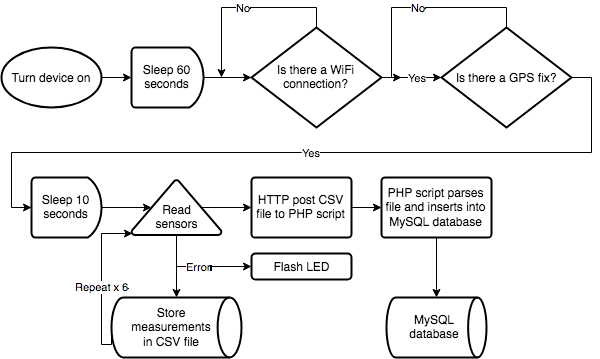
\includegraphics[width=0.9\textwidth]{images/code_flow}
\caption[Flow diagram of system code.]{Flow diagram of system code.}
\label{code_flow}
\end{figure}

\subsubsection{GPS}

Geo-location functionality is provided by a USB GPS module, specifically a GlobalSat BU-353S3 USB GPS Receiver. This plugs directly into one of the RPi's USB ports and appears as the device \texttt{ttyUSB0}. The GPSD protocol, which is built on top of JSON, is used to communicate with the GPS receiver. Responses from the GPS receiver are JavaScript Object Notation (JSON) objects. The \texttt{gpsd} python module is used to interface with the GPSD protocol, parsing the JSON to output longitude and latitude coordinates, as well as other useful information such as horizontal speed and altitude. Installation instructions are detailed in Appendix \ref{GPS}.

Moreover, the RPi is configured to use the GPS receiver as a Network Time Protocol (NTP) time server. This involves the use of the NTP daemon. Installation instructions are detailed in Appendix \ref{NTP}. By enabling this, the RPi syncs its internal clock with an accurate source -- the GPS satellites. This overcomes the issue of the Raspberry Pi having no real time clock, which otherwise can lead to inaccurate timing when recording measurements because the RPi is oblivious to time lapsed since the previous shutdown.

Initially, the project was going to develop an Android application that merged readings from the RPi with GPS data, because the RPi does not have a built-in GPS receiver. The application was created using Android Studio for Mac OSX. The application works by connecting the RPi to the Android phone via Bluetooth, and then uses \texttt{ObexFTP} to send the CSV files from the RPi to the phone. The application then watches a particular directory for new files and upon receipt matches up timestamps in the CSV file with GPS-timestamp pairs stored on the phone, before HTTP posting the file to the server. However, this was a far from ideal solution and introduced tight coupling between the RPi and the phone. Once it was realised that a USB GPS module was available, the Android application was shelved.

\nomenclature{FTP}{File Transfer Protocol}

Although not used in the final version of the device, this development shows that it is possible for the same functionality to be achieved using Bluetooth. It also demonstrates the ability to still collect GPS location data when the Raspberry Pi does not have GPS itself and no GPS module is available. Since the cost of the GPS module is \textsterling 30.99, this alternative solution can be used in an even lower cost version of the device.

% Add installation instructions to the Appendix.

\nomenclature{JSON}{JavaScript Object Notation}
\nomenclature{NTP}{Network Time Protocol}

\subsection{Server-side software and database} \label{server_software}

In order to connect the air quality monitoring device and the database, a client-server architecture is used. A RESTful API receives the CSV files, parses them and then inputs the file's data into a database.

\subsubsection{RESTful API}

A RESTful API written in PHP receives the HTTP posted CSV file, then parses the contents and inserts each line into a row of the database table that stores all measurements. If this completes with no errors, it then also inserts a new row into a system monitoring table with information about the CSV file and time of insertion. If there is an error, a flag is raised in the table that can then be reviewed to ascertain the cause. Appendix \ref{php_api} shows the API code.

\nomenclature{REST}{Representational State Transfer}

\subsubsection{Database}

The University of Bath provides a database hosting service to members of the university. The database software is MySQL version 5.7.16 Community Server. One of these databases is used in this project, containing two main tables: (i) a table that stores the air quality data, and (ii) a table that stores system monitoring information. We are able to only use one table for storing the measurements as the number of rows is low enough to not cause performance issues. The system monitoring table allows identification if and when an error occurs in the data flow.

% Describe tables here %%%%%%%

\subsection{Web application} \label{web_application}

The web application is written in R and uses R Shiny version 1.1.0 to provide the web framework. An example page from the web application is shown in Figure \ref{rshiny}.

\begin{figure}[!tb]
\centering
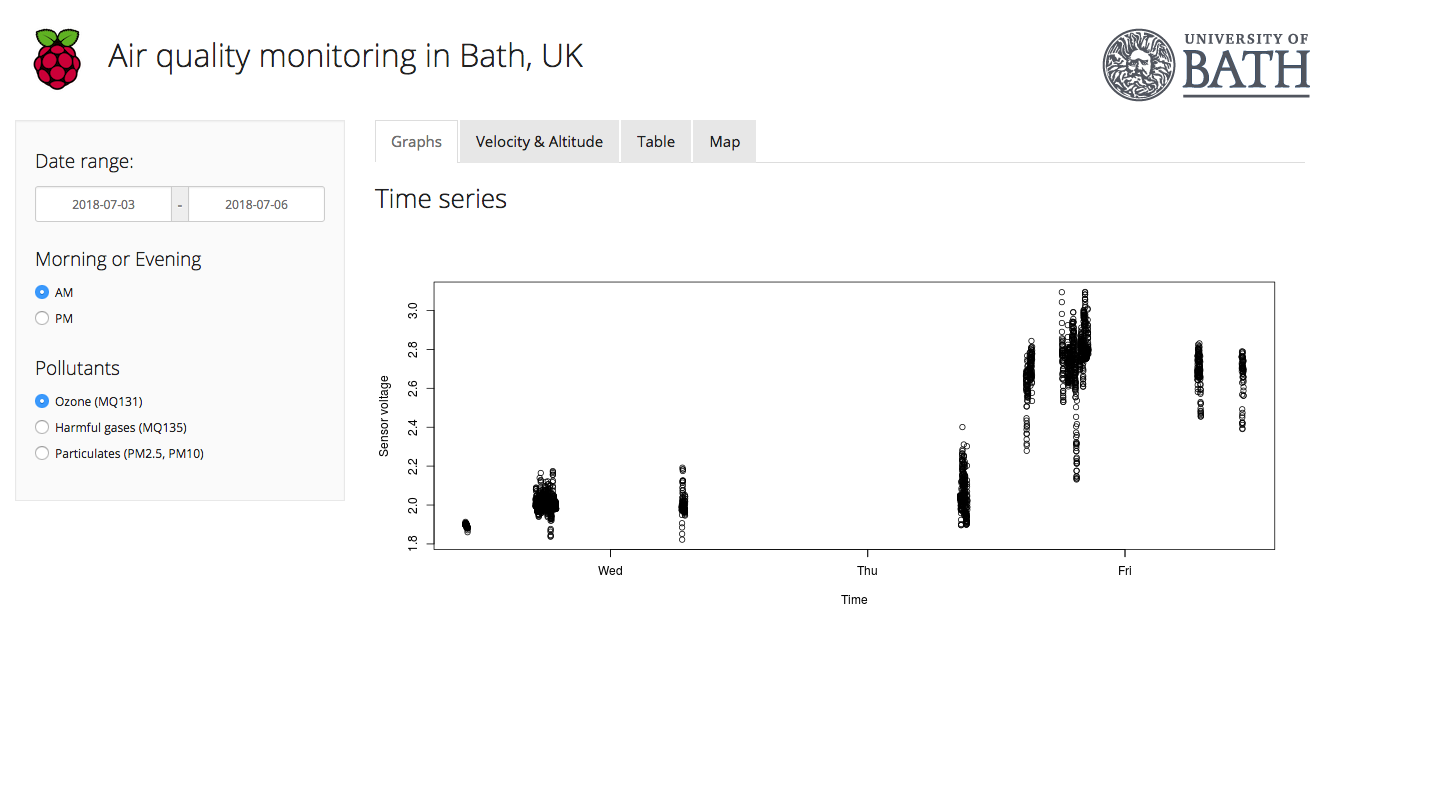
\includegraphics[width=1\textwidth]{images/web_app}
\caption[Web application.]{Web application using R Shiny. The menu on the left-hand side allows the user to select the time period and pollutant, as well as whether outliers should be included in the graphs or not. There are 4 tabs to the webpage, which each display a variety of graphs and tables to the user.}
\label{rshiny}
\end{figure}
% UPDATE IMAGE

The web page's main requirement is to display the information in an easily accessible and understandable manner, so that any member of the public is able to analyse the pollution in their area. It predominantly displays the pollution maps of Bath and line graphs for the time series of data. On the left-hand side of the page is a menu bar that allows the user to select their chosen time period, with the graphs dynamically updating as the selection changes. In addition, there is a dynamic table that displays all of the raw data, with a button for downloading the dataset as a CSV file.


%%%%%%%%%%%%%%%%%%%%%%%%%%%%%%%%%%%%%%%%%%%%%%%%%%%%%%%%%%%%
%%%%%%%%							CALIBRATION					      		       %%%%%%%%
%%%%%%%%%%%%%%%%%%%%%%%%%%%%%%%%%%%%%%%%%%%%%%%%%%%%%%%%%%%%

\chapter{Output conversion and calibration} \label{chap: calibration}

The previous chapter detailed how the device was constructed and provided a high-level description of the software design, although it did not focus on how the sensor outputs were read and interpreted at the low-level.

Sensors either output an analog or digital signal. If the signal is analog, an analog-to-digital converter (ADC) needs to be used to make the output binary (low or high voltage). The communication protocol then must be studied in order to understand how the digital signal can be read in order to get a meaningful signal, instead of reading randomly on the relevant GPIO pin. Once the binary value has been recorded, it then needs to be converted to a decimal value.

The second stage is then interpreting this decimal value and working out how it relates to a meaningful reading. For example, we may read a value of 2048 from a sensor, which could correspond to 2.5V, but the voltage then needs to be mapped to a concentration of a gas.

This chapter details how these processes were created for each of the sensors used in this project and is relatively low-level in comparison to the other chapters.
%If the sensor outputs an analog signal, the ratio of the outputted decimal value to the maximum possible value will correspond to a voltage e.g. $(2048 \divide 4096) \times 5V = 2.5V$. If the sensor outputs a digital signal, it is likely that this value is the 

%\section{Output conversion}

%All of the sensors used in this project do not immediately output an interpretable measurement in terms of units. Therefore, each of the outputs need to be converted. The process carried out for each of the sensors is detailed below.

\section{Particulate sensor}

The output of the Shinyei PPD42NS particulate sensor is a digital pulse. To infer the measured concentration, a value called the Low Pulse Occupancy (LPO) time is calculated. This is the percentage of time over a fixed period that the digital output of the sensor is 'low' (i.e. 0). The LPO can then be used to calculate the estimated number of particles per 0.01 cubic feet using the following equation, which is obtained by digitising the data sheet calibration curve:
\nomenclature{LPO}{Low Pulse Occupancy}
\begin{equation}
\label{LPOtoCF}
y = 1.1x^3 - 3.8x^2 + 520x + 0.62
\end{equation}

However, the DustTrak reference sensor outputs measurements in $\mu g/m^3$, which is an SI unit, meaning the $y$ values from equation \ref{LPOtoCF} need to be converted to this unit. An algorithm was developed by \cite{uva2009preliminary} that achieves this by estimating average particle size and density. It must be stressed that this conversion is only an approximation, because it is impossible to precisely infer the properties of each of the thousands of microscopic particles being counted. The main assumptions are that all particles are spherical with average radius $r$ and density $d$:
\begin{equation}
r = 0.44 \times 10^{-6} m
\end{equation}
\begin{equation}
d =  1.65 \times 10^{12} \mu g/m^3
\end{equation}

From these assumptions, the volume $v$ of a sphere (particle) can be calculated approximately:
\begin{equation}
v = \frac{4}{3} \pi r^3 = 3.568 \times 10^{-19} m^3
\end{equation}

The mass $m$ of a particle is its density multiplied by its volume:
\begin{equation}
m = d \times v = 0.589 \times 10^{-6} \mu g
\end{equation}

Therefore, the mass of particles per cubic foot is calculated by multiplying the mass of a particle $m$ by the number of particles per cubic foot $y$. It is then a simple conversion from cubic feet to cubic metres by multiplying by a factor of $3531.5$.
\begin{equation}
\mu g/m^3 = y \cdot m \cdot 3531.5
\end{equation}

%Additionally, there is a humidity and temperature adjustment, described in Equation \ref{eq:temphumconv}. $O$ is the output of the initial conversion from particle count to concentration (described above), $H$ is the relative humidity percentage, $C$ is the correction factor, and $F$ is the final adjusted output concentration.
%\begin{equation} \label{eq:temphumconv}
%F = O \times H \times C
%\end{equation}
%
%Table \ref{humtemp} shows the values of $H$ and $C$ in normal conditions.
%
%% CHECK IF THIS IS CORRECT AND/OR NEEDED
%
%\begin{table}[!htbp]
%  \centering
%  \caption{Humidity and temperature factors}
%  \label{humtemp}
%  \begin{tabular}{ l l }
%  \toprule 
%  H & C \\ \midrule
%  0-39\% & 13 \\
%  40-49\% & 8 \\
%  50-59\% & 6 \\
%  60-69\% & 4 \\
%  70-79\% & 1.75 \\
%  80-89\% & 1.5 \\
%  90-100\% & 1 \\  \bottomrule
%  \end{tabular}
%\end{table}

\section{Ozone sensor} \label{mq131_calibration}

The output of the MQ131 ozone sensor is a raw analog signal that represents voltage, with the voltage proportional to the quantity of the gas being sensed. Given that the RPi cannot read an analog signal (digital only), an ADC chip is included on the MikroElektronika sensor board. The ADC is an MCP3551, which is a single-channel 22-bit ADC chip. The communication between the RPi and this ADC is via a serial communication. More specifically, a Serial Peripheral Interface (SPI). This is a synchronous serial communication interface consisting of an SPI master and SPI slave relationship, which is visualised in Figure \ref{spi}.

\begin{figure}[!tb]
\centering
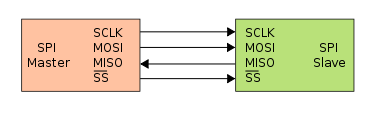
\includegraphics[width=0.8\textwidth]{spi_master_slave}
\caption[SPI master-slave design.]{SPI master-slave design. This visually depicts the relationship between a single master and a single slave on a Serial Peripheral Interface (SPI) bus. (SCLK = Serial Clock, MOSI = Master Output Slave Input, MISO = Master Input Slave Output, SS = Slave Select.)}
\label{spi}
\end{figure}

Each data word is made up of 24 bits (3 bytes): 22 bits of conversion data and 2 additional overflow bits. To read from the MCP3551, the RPi must detect when the chip is ready, indicated with $\overline{CS}$ (Chip Select) low on the $SDO/\overline{RDY}$ (Data Output) pin. Conversely, a high state ($\overline{CS}$ held high) indicates the device is busy converting. When reading from the ADC, the data is passed Most Significant Bit (MSB) first -- this is the bit in the binary number with the highest numerical value. If these 24 bits are indexed as bit 23 to bit 0, then bit 23 and bit 22 are the overflow bits, bit 21 is the sign bit (indicates positive or negative), and bits 20 to 0 contain the 21-bit value. Excluding the overflow bits, values therefore range from \SI{-2097152} ($2^{21}$) to \SI{2097151}. This information is visualised below in Figure \ref{mcp3551}.

\nomenclature{SPI}{Serial Peripheral Interface}
\nomenclature{MSB}{Most Significant Bit}

\begin{figure}[!htb]
\centering
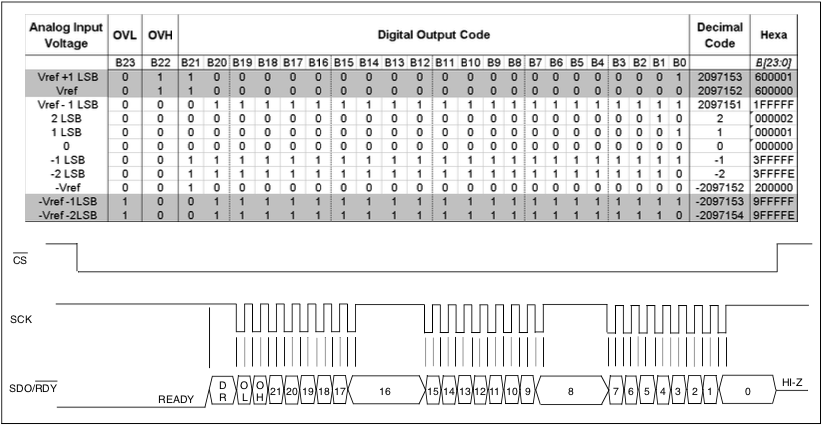
\includegraphics[width=1\textwidth]{mcp3551}
\caption[MCP3551 output codes.]{Summary of output coding data format. This shows example digital output codes for specific analog input voltages when using a typical SPI communication. [REF]}
\label{mcp3551}
\end{figure}

Once the RPi has read the ADC value, this value is then converted to a decimal value using a binary-to-decimal conversion. The output voltage of the sensor is a value between 0 and 5V. Since the range of decimal values is \SI{-2097152} to \SI{2097151}, the decimal value $d$ needs to be converted to a fraction and then multiplied by 5V to get the voltage output value $V_{IN}$.
\begin{equation}
V_{IN} = \frac{d + 2097152}{4194304} \cdot V_{REF}, \hspace{5mm} V_{REF} = 5V
\end{equation}

\begin{figure}[!htb]
\centering
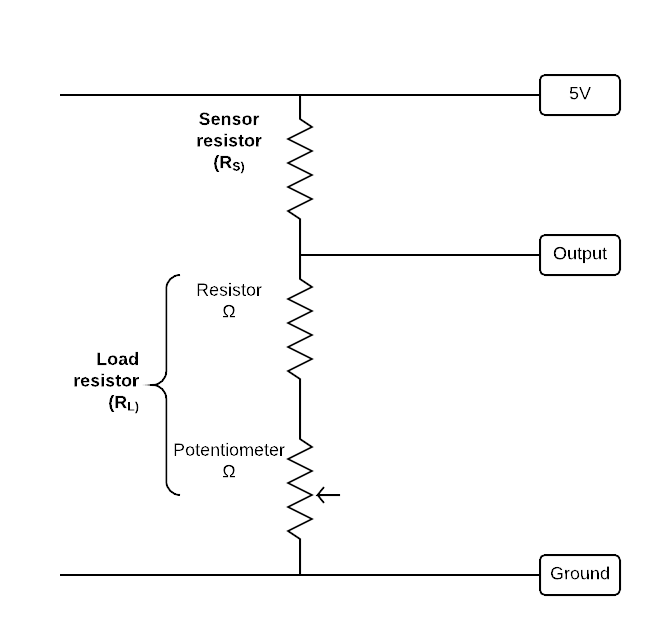
\includegraphics[width=0.6\textwidth]{circuit}
\caption[Circuit diagram for MQ-series sensors.]{Circuit diagram for MQ-series sensors. This shows how the sensor uses $R_S$ and $R_L$ to make a voltage divider. [EDIT]}
\label{circuit}
\end{figure}

Using the calibration curves on the MQ131 sensor data sheet (Figure \ref{mq131_curve}), it is possible to calculate an approximate ozone reading in $\mu g/m^3$. The first part of the calculation is based on the circuit structure (Figure \ref{circuit}) and requires the resistance of the sensor (R\textsubscript{S}) in clean air (R\textsubscript{0}). Unfortunately, there are no controlled ozone environments available at the university for calibrating the sensor. Therefore, we assume that the indoor air was clean and contained minimal ozone. To calculate R\textsubscript{0}, set the sensor's potentiometer to its minimum resistance ($0\Omega$) and record the output voltage $V_L$. Then, also set the potentiometer to its maximum resistance ($10k\Omega$) and record the output voltage $V_H$. Figure \ref{potentiometer} shows the potentiometer of both the MQ131 and MQ135 sensors. Once the output voltage at these two points has been recorded, it is possible to calculate R\textsubscript{0} by using the following equation:
\begin{equation}
V_{OUT} = V_{IN} \cdot \frac{R_L}{R_0 + R_L}, \qquad V_{IN} = 5V
\end{equation}
which can be rearranged to
\begin{equation}
R_0 = (\frac{V_{IN}}{V_{OUT}} - 1) \cdot R_L
\end{equation}
In fact, there are two equations since we have two different pairs of $R_L$ and $V_{OUT}$.
\begin{equation}
R_0 = (\frac{5}{4.934} - 1) \cdot 10100 = 135.103 , \quad R_0 = (\frac{5}{2.015} - 1) \cdot 100 = 148.139
\end{equation}
Theoretically, these calculated $R_0$ values should be the same, but here we take the average as they differ slightly (likely due to their low cost).
\begin{equation}
\therefore R_0 = \frac{135.103 + 148.139}{2} = 141.6
\end{equation}

\begin{figure}[!tb]
\centering
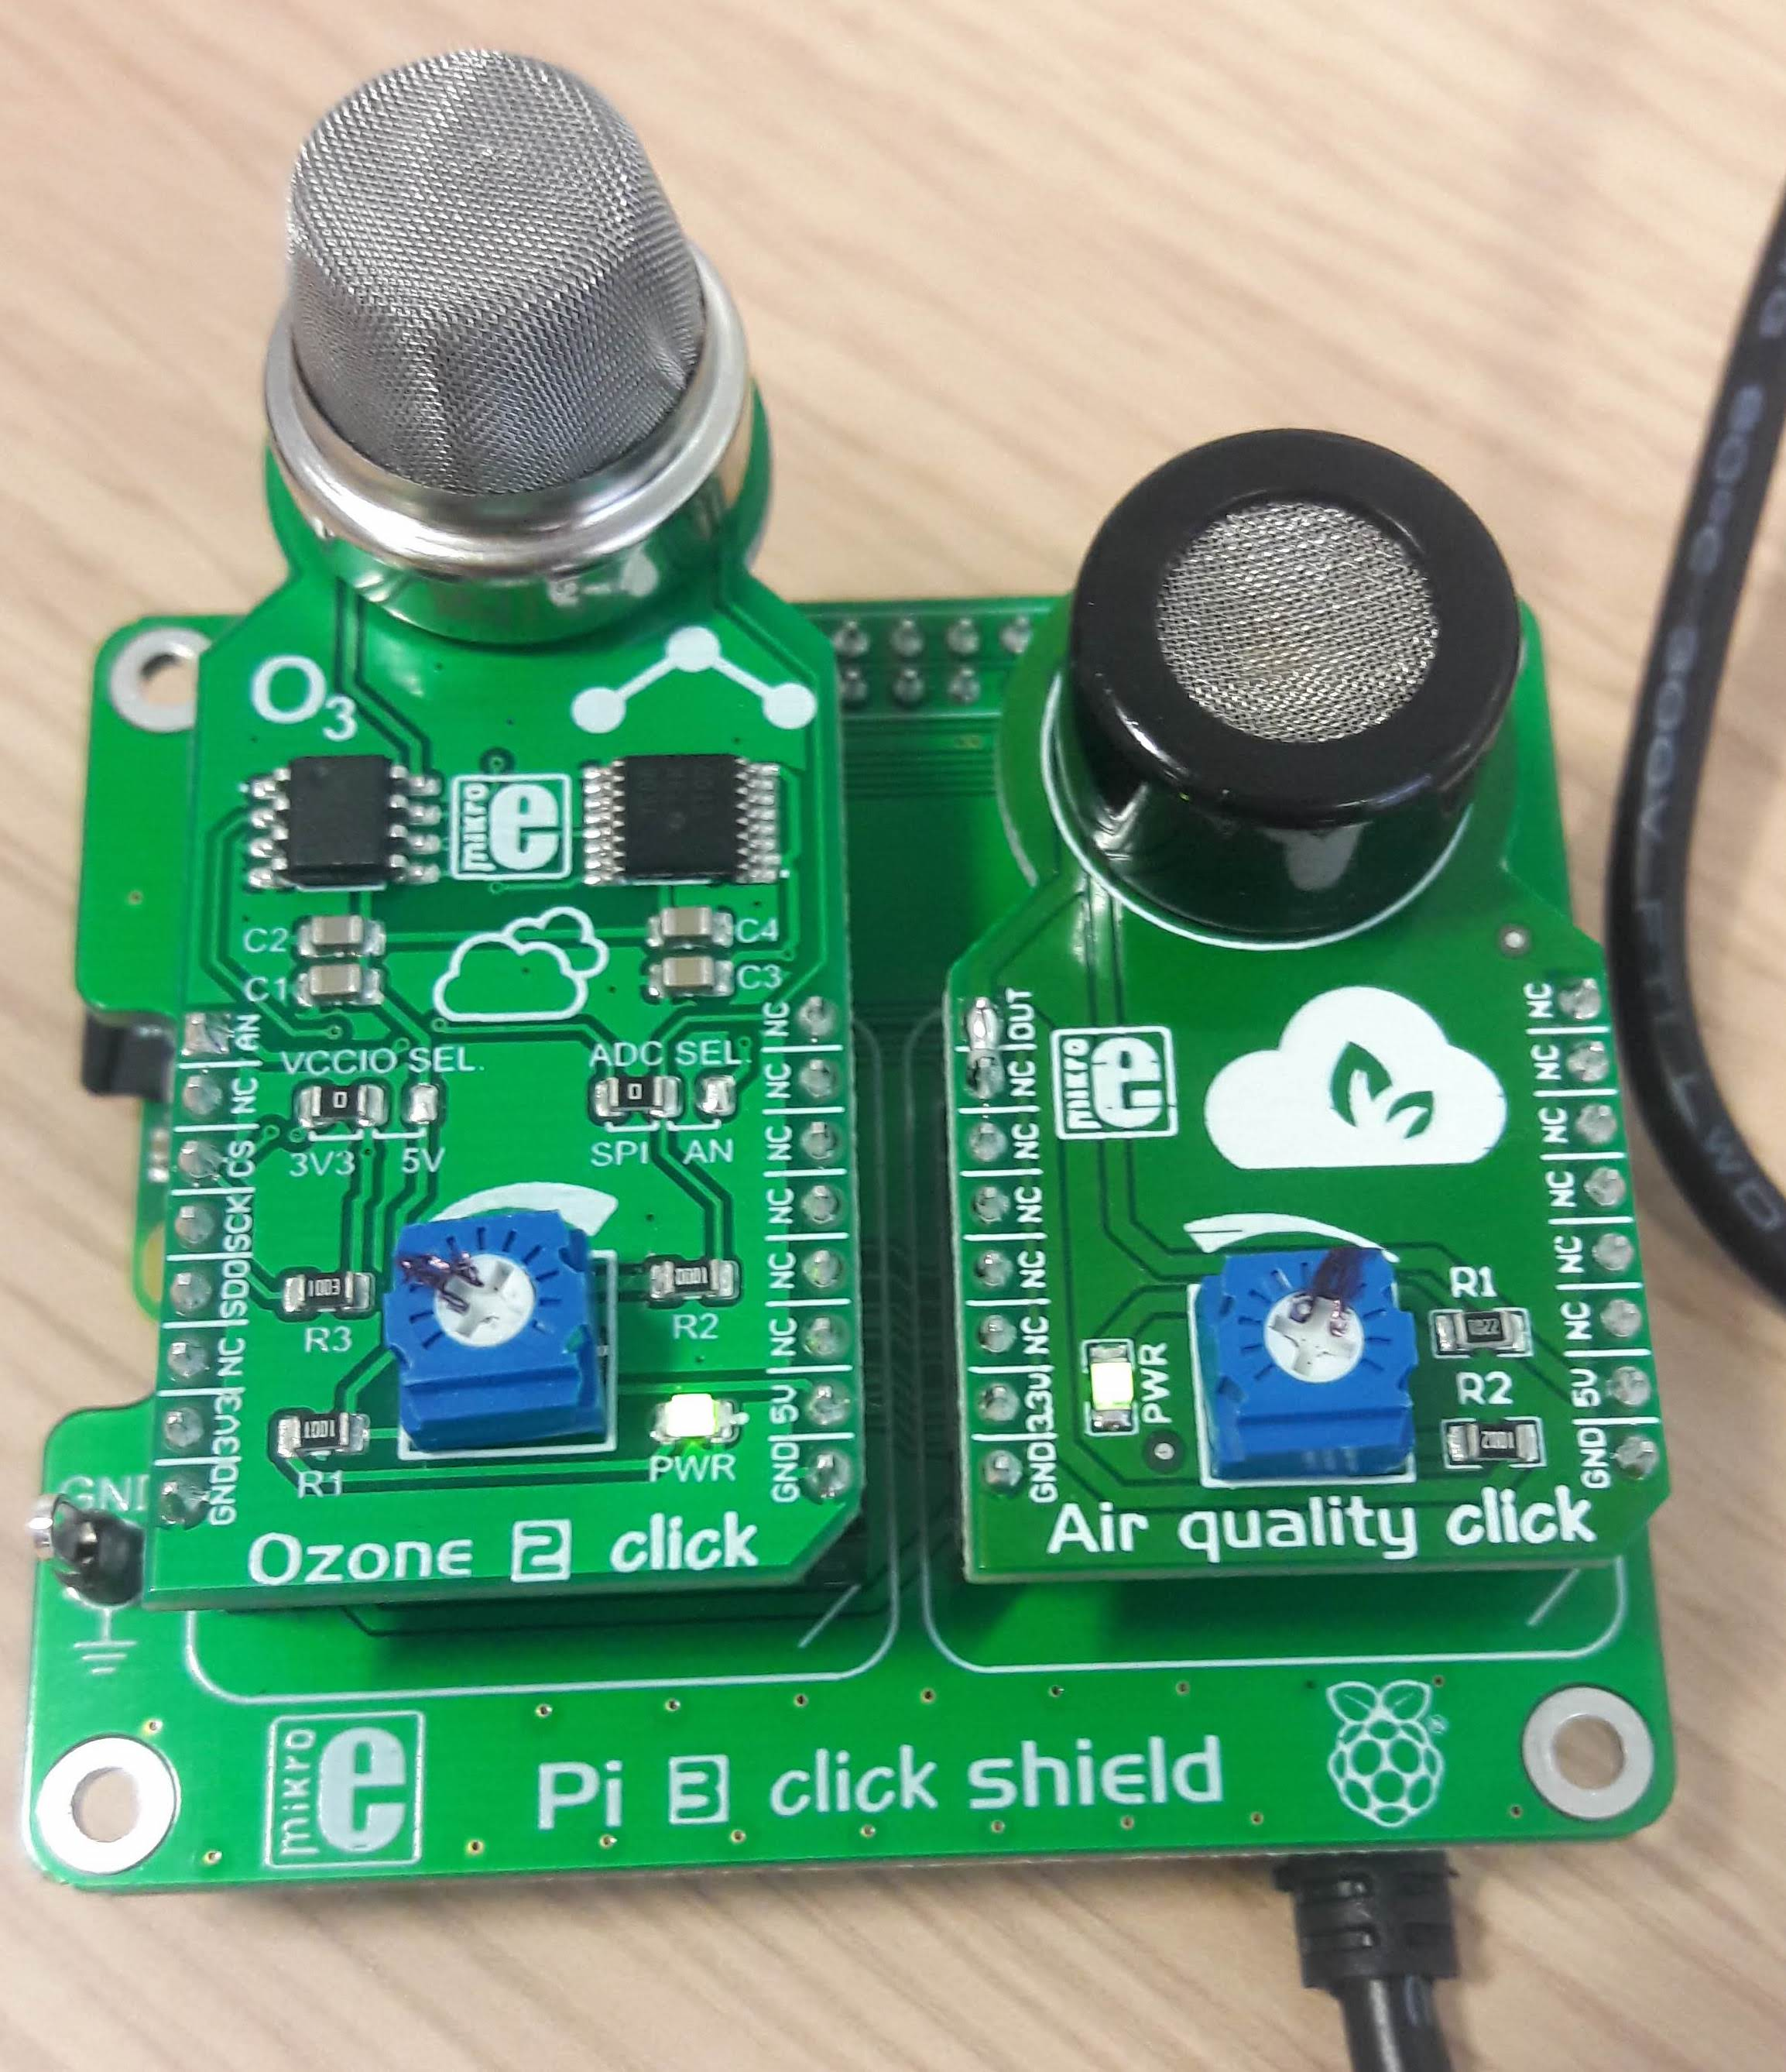
\includegraphics[width=0.4\textwidth]{potentiometer}
\caption[MikroElektronika potentiometers]{MikroElektronika click board potentiometers. (L) blue potentiometer of ozone click (MQ131); (R) blue potentiometer of air quality click (MQ135).}
\label{potentiometer}
\end{figure}

%Using R\textsubscript{0}, it was then possible to calculate the resistance of the sensor R\textsubscript{S} in any environment using the following equation:
Since we now know $R_0$, we can set the potentiometer so the output voltage is reasonable (i.e. around a mid-point) and then work out the corresponding load resistance $R_L$:
\begin{equation}
R_L = \frac{V_{OUT} \cdot R_0}{V_{IN} - V_{OUT}}
\end{equation}
Then in any environment, it is possible to calculate $R_S$:
\begin{equation}
R_S = (\frac{V_{IN}}{V_{OUT}} - 1) \cdot R_L
\end{equation}
This enables the calculation of the ratio R\textsubscript{S}/R\textsubscript{0}, which can be inputted into the calibration curve (Figure \ref{mq131_curve}) to output an approximate ozone reading in $\mu g/m^3$. We digitise the calibration curve to obtain $(x, y)$ pairs and then use power regression to obtain the final equation:
\begin{equation}
O_3 (ppb) = (0.0541 \frac{R_S}{R_0}) ^ {(-\frac{1}{0.917})}
\end{equation}

\begin{figure}
\centering
\begin{subfigure}[b]{0.45\textwidth}
  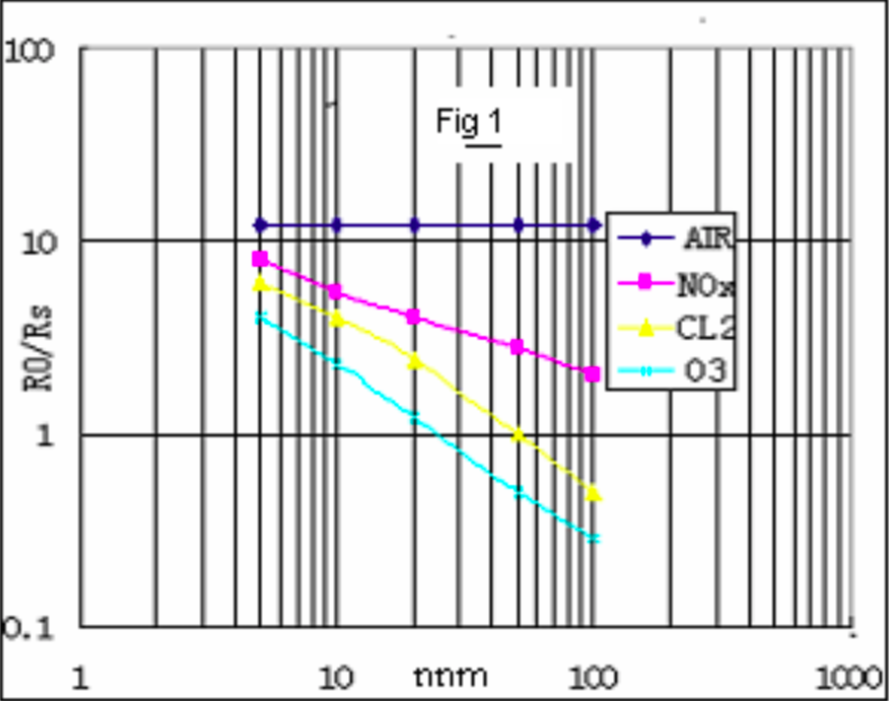
\includegraphics[width=\textwidth]{ozone_data_sheet}
  \caption{MQ131.}
  \label{mq131_curve}
\end{subfigure}
\hfill
\begin{subfigure}[b]{0.45\textwidth}
  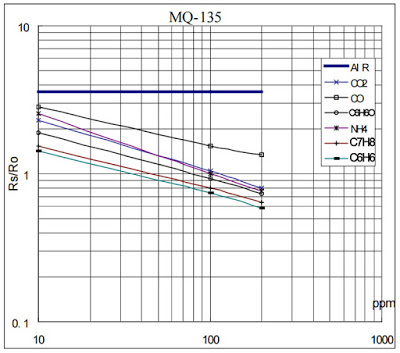
\includegraphics[width=\textwidth]{mq135_data_sheet}
  \caption{MQ135.}
  \label{mq135_curve}
\end{subfigure}
\caption[Calibration curves.]{Calibration curves from sensor data sheets. (a) shows the calibration curve for the MQ131 sensor, with ozone being the light blue line, and (b) shows the calibration curve for the MQ135 sensor, with a number of different sensitivities.}
\end{figure}


\section{General air quality sensor}

The MQ135 air quality sensor also outputs a raw analog signal that represents voltage. To avoid repetition, only the differences in the ADC chip used are explained here, with the rest of the process following that described above for the MCP3551 chip.

The Air Quality Click from MikroElektronika did not contain a dedicated ADC chip, unlike the Ozone Click. Therefore, a Mikro Pi 3 Click Shield HAT is used, which provides a GPIO/ADC switch so the relevant option can be selected. The switch for the Ozone Click is set to GPIO since it has an in-built ADC, whilst the switch for the Air Quality Click is set to ADC, thus routing the sensor's output through the ADC (see Figure \ref{fig:switch}). The Pi 3 Click Shield uses an MCP3204, which is a 4-channel 12-bit ADC chip. As with the MCP3551, the communication with the RPi uses SPI and each data word is made up of 3 bytes. Initiating communication is also achieved by bringing the $\overline{CS}$ low. However, they differ in their data transfer protocol. The RPi (SPI master) must first send configuration bits to the MCP3204: 5 leading zeroes, a start bit (1) and then 4 configuration bits. The ADC then samples the analog signal for 1 clock cycle, before responding with 1 null bit and then the data over the next 12 bits, MSB first.

\begin{figure}[!tb]
\centering
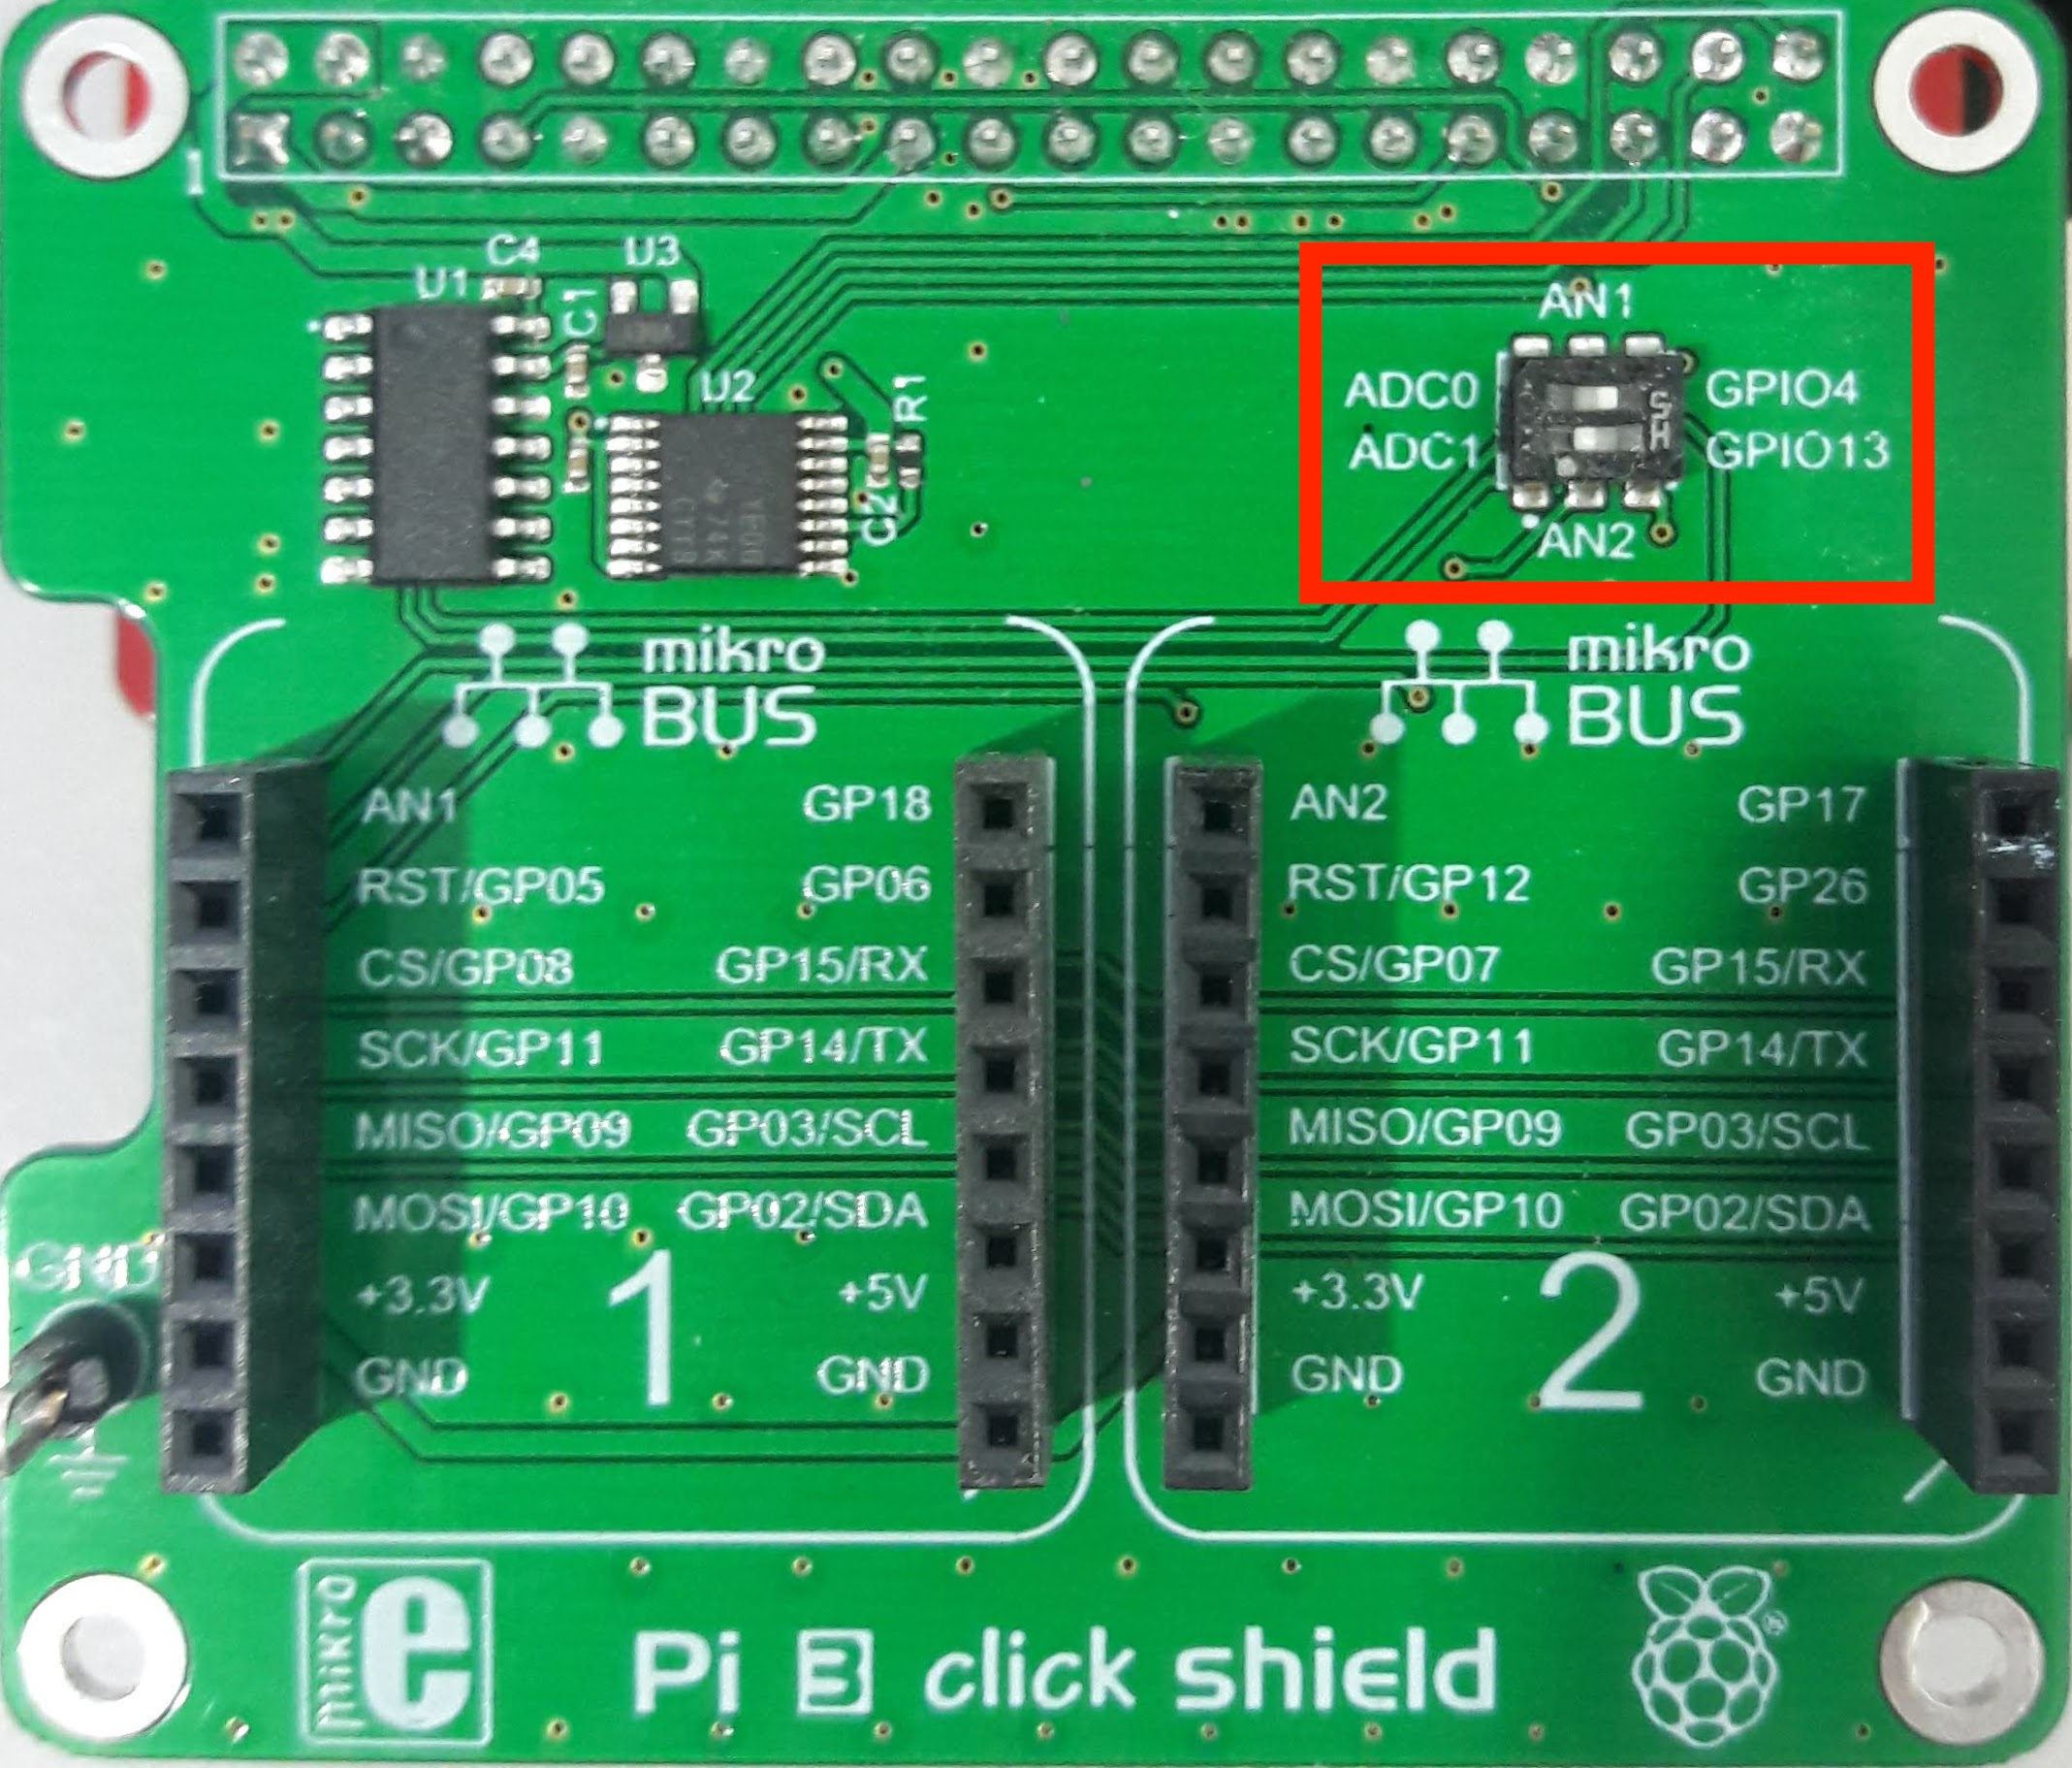
\includegraphics[width=0.4\textwidth]{images/gpio_adc_switch}
\caption[GPIO/ADC switch.]{GPIO/ADC switch. The switch is highlighted in red on the Mikro Pi 3 Click Shield HAT. This switch enables the signal to either be sent directly to the GPIO pins or directed to the ADC first.}
\label{fig:switch}
\end{figure}

These 12 bits allow for a range of digital values between 0 and 4095. Again, the decimal output $d$ from the ADC needs to be converted to a fraction and then multiplied by 5V to get the voltage output value $V_{IN}$.
\begin{equation}
V_{IN} = \frac{d}{4096} \cdot V_{REF}, \hspace{5mm} V_{REF} = 5V
\end{equation}

A similar calibration process can be attempted, but using the calibration curve in Figure \ref{mq135_curve} instead. However, this graph does not detail NO\textsubscript{x} on any of the calibration curves, despite the sensor description detailing it is sensitive to NO\textsubscript{x}. Upon further research, it was found that the MQ135 sensor is actually sensitive to a number of different gases that indicate poor air quality, including ammonia, nitrogen oxides, benzene, smoke, carbon monoxide and carbon dioxide. However, it is impossible to isolate any of these gases from the signal without further equipment. Therefore, much of the analysis herein for this sensor focuses on the raw voltage output and only the voltage delta can be analysed, with no precise NO\textsubscript{x} relation. Essentially, the voltage acts as a `basket' measure of air quality.
% As an alternative, we attempt a carbon monoxide calibration from the voltage reading. However, this appears to be inaccurate.

\section{Temperature and humidity sensor}

The output of the DHT22/RHT03 temperature and humidity sensor is a digital signal. The sensor uses a single-bus for communication, where the sensor is the slave and the computer is the master. Each data word is made up of 40 bits: 16 bits for the humidity reading, 16 bits for the temperature reading and the final 8 bits as a check-sum. The humidity and temperature readings are split into two parts: the first byte is the integer part and the second byte provides the fractional part. To read from the DHT22, the RPi must send a read command (pull low for $18\mu s$, pull high for $20-40\mu s$) and then the sensor replies with an acknowledgement (pull low for $80\mu s$, pull high for $80\mu s$). The data transfer then follows, with $50\mu s$ low for a 0 and $70\mu s$ high for a 1. The data is sent MSB first. Binary-to-decimal conversion is used to convert the binary values to temperature readings in Celsius and humidity values in percentage form.

\begin{figure}[!tb]
\centering
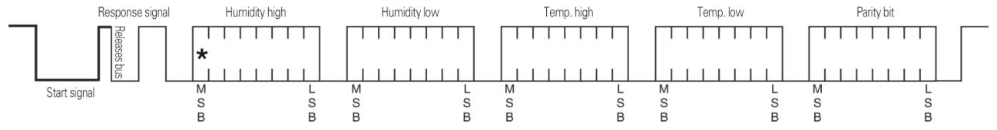
\includegraphics[width=1\textwidth]{images/dht22_data}
\caption[DHT22 communication protocol.]{DHT22 communication protocol. The data word is made up of 40 bits: 16 bits for the humidity reading, 16 bits for the temperature reading and the final 8 bits as a check-sum.}
\label{dht22_data}
\end{figure}

\section{Limitations}

One of the shortcomings of our calibration process for the Shinyei PPD42 particulate sensor is it assumes particle shape and size. It could be possible to use pulse-width modulation (PWM) to record the size of particles that pass in front of the sensor's detection beam, although this may be inaccurate due to the sensor's inability to isolate individual particles. Despite the increase in cost, other particle detection methods (e.g. gravimetric measurement) may provide more precise measurement of particulate concentrations.

Furthermore, there are no known concentrations of ozone gas available at the university, meaning we cannot measure the output voltage of the MQ131 sensor at specific concentrations of ozone. As a result, we cannot plot points at different concentrations to create our own calibration curve. Instead, we are forced to use the data sheet's calibration curve, which may be inaccurate.

Similarly for the MQ135, we do not have access to known concentrations of NO\textsubscript{x} in the sensor's detection range. We did manage to test the sensor output using 500~ppm NO\textsubscript{x} gas in the university's Automotive Research Group laboratory. However, this concentration was far greater the normal range of NO\textsubscript{x} found in the atmosphere and so overwhelmed the sensor. Moreover, the aforementioned issue relating to the sensor's multi-functionality means we cannot calibrate the voltage to a specific concentration of a single gas. This means the device cannot definitively identify variations in NO\textsubscript{x}, but nonetheless is still useful in identifying poor general air quality.

\nomenclature{ppm}{Parts-per-million}

Moreover, because these sensors are low-cost, they have cross-sensitivities with other atmospheric gases that can potentially cause unwanted changes in sensor output. However, without the correct testing equipment or more expensive sensors that only have very minimal cross-sensitivities, it is not possible to correct for these effects in the time frame of this project. This is unfortunately a common issue when using low-cost sensors, hence their price.

It is also worth noting that the data sheets for these sensors indicate that their outputs can drift over time, which has also been found by previous studies [REF]. Our data collection period is 2 weeks, which is too short to notice a change as they typically occur over bi-annual or annual periods of time. However, this effect should be tested and accounted for if the device is to be used for longer periods of time.

%%%%%%%%%%%%%%%%%%%%%%%%%%%%%%%%%%%%%%%%%%%%%%%%%%%%%%%%%%%%
%%%%%%%%							Question 1					      		       %%%%%%%%
%%%%%%%%%%%%%%%%%%%%%%%%%%%%%%%%%%%%%%%%%%%%%%%%%%%%%%%%%%%%

%\renewcommand{\chaptermark}[1]{%
%\markboth{\MakeUppercase{%
%\chaptername\ \thechapter.%
%\ #1}}{}}

\chapter[Bicycle-based monitoring]{Question 1: Can air pollution be monitored to a satisfactory level using a bicycle-based monitoring device?} \label{chap:q1}

Chapters \ref{chap: system_design} and \ref{chap: calibration} detailed how the air quality monitoring device, and system as a whole, was constructed and how the sensors were calibrated to output meaningful values. These chapters collectively described the process undertaken in creating the final device, providing a product that can now be used to answer our research questions.

This chapter focuses on the first research question: whether air pollution can be satisfactorily monitored using a bicycle-based monitoring device. Section \ref{meth:q1} details the methodology behind how the device is applied to answer this research question. Each method is described in detail, with our reasoning provided in each case to support our choices. Section \ref{results:q1} then displays the results and analyses the findings.

\section{Methodology} \label{meth:q1}

The methodology is structured as follows. The first three parts focus on where and how the data is collected, which includes the location choice (Section \ref{location}), the selection of the route (Section \ref{route_selection}) and the data collection method (Section \ref{data_collection:q1}). In order to then answer the research question, a number of distinct parts need to be considered. Firstly, the optimal positioning of the device on the bicycle needs to be considered (Section \ref{position_testing}). Secondly, the quality of the data from this device must be assessed to test whether it is satisfactory and any necessary changes made (Section \ref{data_quality}). Thirdly, the data from the device needs to be tested to see whether it can detect variations and patterns in the pollution ... [RE-WORD]

%In order to answer this research question, three distinct parts need to be considered. Firstly, data needs to be collected along a consistent route for a suitable period of time so as to encompass varying environmental conditions. By analysing the sensor outputs under these different conditions, we can test whether the device can identifying trends/differences in air pollution. Secondly, different positions of the device on a bicycle need to be considered. Finally, the optimal method of inducing air flow over/into the air quality sensors needs to be analysed. % CHANGE

\subsection{Location} \label{location}

Given this project is being conducted at the University of Bath, we carry out the data collection in the city of Bath, UK. In addition to the proximity to the university, the city is also chosen for its traffic and pollution problem, which has led to the creation of the Bath Air Quality Action Plan \citep{BANES2017baqap}. This plan, created by the Bath and North East Somerset (BANES) council, sets out how an improvement in the air quality in Bath will be achieved between 2017 and 2022. This document is a requirement from the government, following BANES being identified by the government as 1 of 23 local authorities `with persistent exceedances required to undertake local action to consider the best option to achieve statutory NO\textsubscript{2} limit values within the shortest possible time' \citep{DEFRA2017uknoxplan}. By collecting air pollution data in Bath, the outputs of this project could help the council better understand pollution in Bath by comparing the council's own fixed monitoring stations with the mobile measurements from this project. This may also identify previously unknown problem pollution areas.

\nomenclature{BANES}{Bath and North East Somerset Council}

Furthermore, Bath is geographically interesting because of its position surrounded by steep hills. These hills act as a channel for wind coming from the west and could potentially direct air pollution into Bath, as well as trapping it in the city. Figure \ref{bath_elevation} shows an elevation raster map of Bath, with the colouring and shading indicating the terrain and altitude.

\begin{figure}[!htb]
\centering
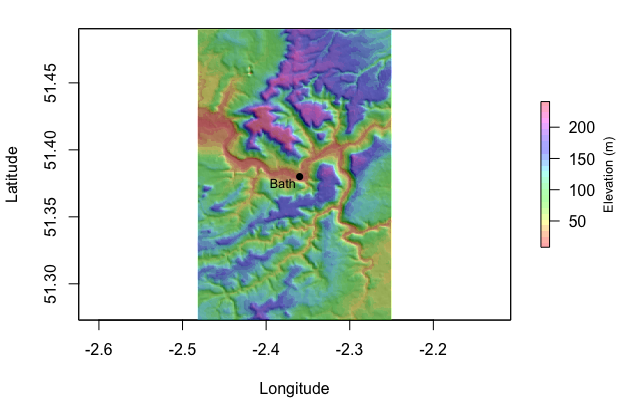
\includegraphics[width=0.9\textwidth]{images/bath_elevation_large}
\caption[Elevation raster of Bath.]{Elevation raster of Bath. This image shows how Bath is surrounded by steep hills to the north, east and south, which act as a funnel for wind and, therefore, air pollution into Bath.}
\label{bath_elevation}
\end{figure}

\subsection{Route selection} \label{route_selection}

The selected route is based upon the current fixed air quality monitoring stations in Bath, so that measurements obtained by this project can be compared to the official council measurements. The locations of these stations are displayed and labelled in Figure \ref{cycling_route}. The cycling route passes by all of these stations, and attempts to follow the main roads where possible as these likely have the highest levels of pollution. This route has also been overlaid on the figure.

\begin{figure}[!tb]
  \centering
  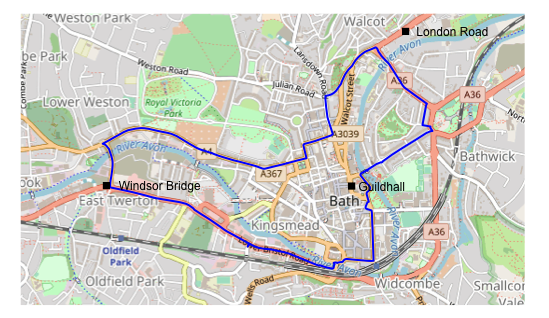
\includegraphics[width=0.7\linewidth]{cycling_route}
  \caption[Cycling route.]{Map of fixed air quality monitoring sites in Bath with the chosen cycling route overlaid. The route passes by all three fixed monitoring stations.}
  \label{cycling_route}
\end{figure}

Furthermore, BANES outlined an `Air Quality Management Area' in 2013. This is shown in Figure \ref{aqma}. Again, the chosen cycling route almost completely falls within this area, thus strengthening our rationale behind the route's choice. By monitoring pollution inside this area, the results will be most useful for the local authority.

\begin{figure}[!tb]
\centering
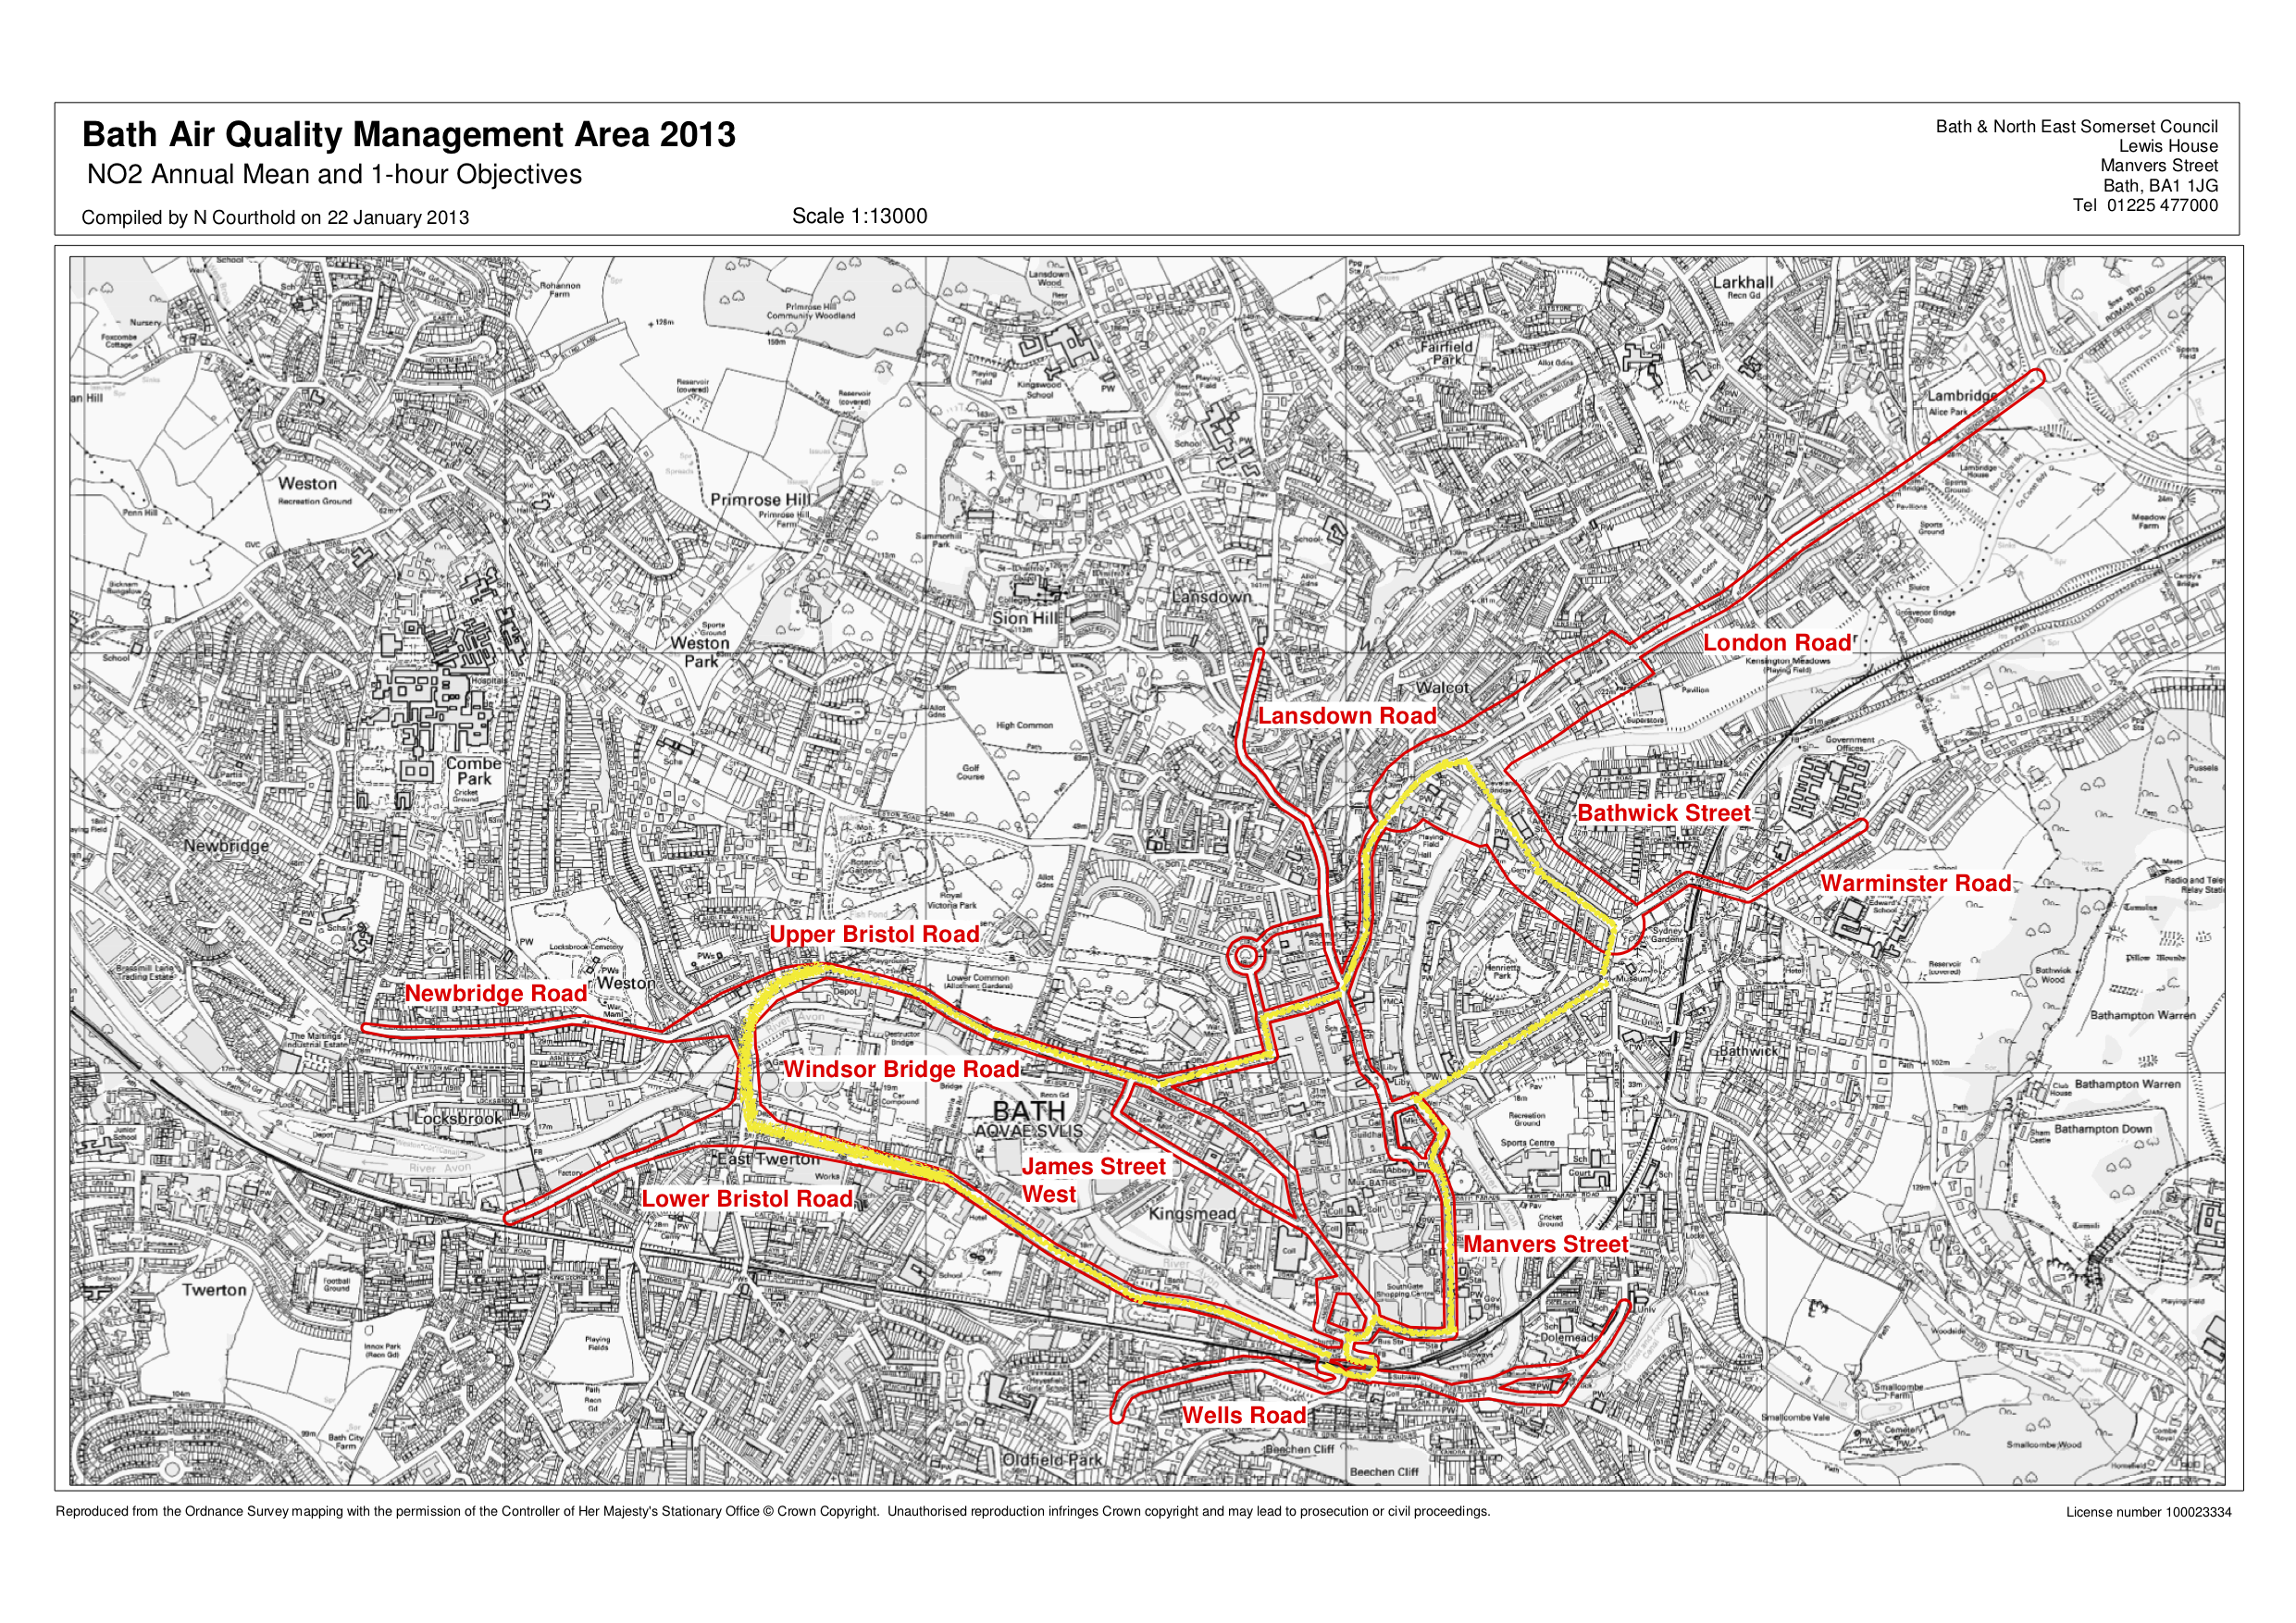
\includegraphics[width=1\textwidth]{shaded_route}
\caption[Bath Air Quality Management Area.]{Bath Air Quality Management Area \citep{BANES2017baqap} with shaded cycling route.}
\label{aqma}
\end{figure}

\subsection{Data collection} \label{data_collection:q1}

To collect data, we ride a bicycle with the air quality monitoring device attached around a pre-determined route, detailed in Section \ref{route_selection}. The route is traversed in both directions in order to help identify anomalous measurements. This leads to minor differences in the route due to certain one-way streets in Bath. We ride the bicycle at a relatively constant speed in order to distribute measurements regularly in spatial terms.

Data is collected across 3 weeks in July and August, from Monday 23rd July to Tuesday 14th August. The route is cycled both in the morning and afternoon. The morning run is to coincide with the morning rush hour and the evening run is to coincide with the evening rush hour. These times are deemed to have the highest pollution levels across the day. 3 weeks is also deemed long enough to allow for weather variations, which allows us to analyse the effect of weather on the measurements.

\subsection{Positioning on bicycle} \label{position_testing}

In order to identify which position on a bicycle is optimal for an air quality monitoring device, we need to test the device attached to different positions. We identify three potential positions on a bicycle, shown in Figure \ref{bicycle_positions}. Position 1 is situated directly below the rider and could potentially be impacted by particles thrown up by the front wheel. It is also not as visible to the user. On the other hand, this position may provide good protection from the elements and help to make the device robust. Position 2 is the least visible, but is situated lowest on the bicycle frame and, thus, provides a different testing environment for the sensor. This may also be impacted by particles thrown up by the wheels. Finally, Position 3 is situated above the front wheel, thus avoiding any particles thrown up by the wheels. In addition, it is the most suitable position for the user to view the device and allows the user to notice when the system-status LED is flashing. 

\begin{figure}[!tb]
\centering
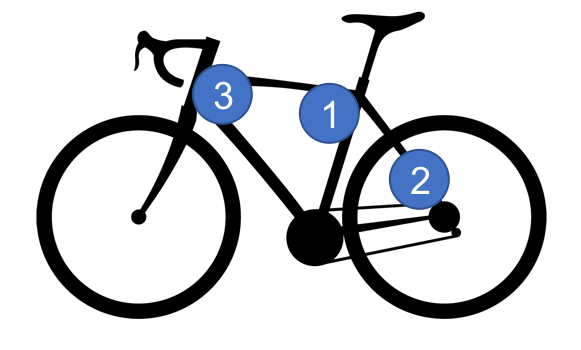
\includegraphics[width=0.6\textwidth]{images/bicycle_positions}
\caption[Device positions on bicycle.]{Potential positions for device on bicycle. (1) is above the front wheel, (2) is directly below the rider, and (3) is on the seat stays.}
\label{bicycle_positions}
\end{figure}

We cycle with the device attached in each position in turn along the same stretch of road. This testing is also carried out across a short time period in order to minimise the effect of changes in the environmental conditions. The results are then compared to ascertain whether the position of the device makes a difference, analysing whether any major spikes occur in the data, which could indicate that the device is being impacted by particulate matter thrown up by the wheels.

\subsection{Data quality} \label{data_quality}

%Data cleaning is the process of transforming raw data into consistent data that can be analysed. The operations carried out influence the statistical properties of the data, meaning they should be conducted with caution and in a reproducible manner.

Whilst ideally our sensors will not output anomalous readings, it is almost inevitable given their low cost. Therefore, it is prudent to detail our approach to cleaning the data outputted by these sensors, especially for future reproducibility. The approach used in this project focuses on the detection and removal of outliers. Outliers are often detected by considering the distribution of values around a mean $\mu$ with standard deviation $\sigma$ and an indicator of the confidence interval $z$:
\begin{equation}
\mu \pm z \times \sigma
\end{equation}

Values that fall outside this range are unlikely to be from the underlying distribution and so can be considered outliers.

However, the mean and standard deviation are not robust to outliers (i.e. the addition of one large erroneous value can disproportionately influence these values). Given we are using low-cost sensors that are more prone to errors than industry-grade sensors, a robust detection method is needed. As a simple check for the presence of outliers, one can examine the distribution of values using a histogram. If some bars are spaced considerably far away from the majority of values, this can indicate outliers are present.

In order to more precisely identify which measurements are outliers in our data, a three-part approach is used. In each case, we apply the outlier detection method and if all of these methods report a reading to be an outlier, it is filtered out from the sample through the use of a type of band pass filter.
\begin{enumerate}
\item Inter-quartile range (IQR)
\item Median and Median Absolute Deviation (MAD)
\item S\textsubscript{n}
\end{enumerate}

These methods are run on three different groupings to assess which is best: (i) on the dataset as a whole, (ii) by time period grouping, and (iii) by a moving time period.

%These outlier detection techniques are then used to create a type of band pass filter in which data outside a calculated range are filtered out.

\subsubsection{IQR} \label{iqr}

The IQR was created by \cite{tukey1977iqr} and provides a measure of statistical dispersion. It is defined as the difference between the 25th and 75th percentiles. Coupled with the 25th and 75th percentiles ($Q_1$ and $Q_3$, respectively), it can be used to define an outlier detection rule. Values outside the range shown in Equation \ref{eqn:iqr} are considered outliers.
\begin{equation} \label{eqn:iqr}
[ Q_1 - 1.5 \times IQR, \quad Q_3 + 1.5 \times IQR]
\end{equation}

\subsubsection{Median and MAD} \label{mad}

The median can be used as a measure of central tendency and is considered to be more robust than the mean, with a breakdown point of 50\% (the proportion of erroneous observations an estimator can handle before giving an incorrect result). This is, in fact, the highest possible breakdown point. The median is defined as the value that separates the distribution into two equal halves.

The median absolute deviation (MAD) can be used as a measure of the variability in the data and is more robust than the standard deviation, with a breakdown point of 50\%. The MAD is calculated by finding the median of absolute deviations about the median. More formally, it is defined as follows:
\begin{equation}
MAD = b \cdot M_i (| x_i - M_j (x_j) |)
\end{equation}
where $M(\cdot)$ is the median function, $x$ is an observation and $b$ is a constant scale factor depending on the distribution.

\nomenclature{MAD}{Median absolute deviation}

These two values can then be used to identify outliers using the following statistic:
\begin{equation} \label{eqn:mad}
\frac{| x_i - M_j(x_j) |}{MAD}
\end{equation}
for each $x_i$ and flagging those $x_i$ which exceed a certain cutoff (typically 2.5 or 3).

%However, the MAD does have drawbacks. Firstly, the MAD takes a symmetric view on dispersion, meaning it can perform poorly on asymmetric distributions (i.e. skewed). Secondly, it has low Gaussian efficiency (approximately 37\%). % potentially remove Gaussian efficiency

\subsubsection{S\textsubscript{n}} \label{sn}

The MAD takes a symmetric view on dispersion, meaning it can perform poorly on asymmetric distributions (i.e. skewed). \cite{rousseeuw1993alternatives} suggested an alternative estimator, $S_n$.
\begin{equation} \label{eqn:sn}
S_n = c \cdot M_i ( M_j | x_i - x_j | )
\end{equation}

Equation \ref{eqn:sn} is very similar to Equation \ref{eqn:mad}, except that the median function $M_j(\cdot)$ has been moved outside the absolute value. The breakdown point of estimator $S_n$ is still 50\%, but it has a better efficiency than MAD.


\subsubsection{Time series} \label{time_series_incorp}

Since our dataset is a collection of time series, the outlier detection should also take this into account. There are two ways we incorporate this into our methodology.

The first way we account for the time series nature is by using a similar method to \cite{vanZoest2018outlierdetection}. The authors appear to be one of the first to create a method for identifying outliers in spatio-temporal air quality data. Their method consists of separating the data into spatial and temporal divisions. For example, urban traffic and urban background (spatial), and weekdays/weekends and traffic times (temporal). The reason for this was that air quality can depend highly on the local area and the time of day, so outlier detection must take these divisions into account. As a result, the spatio-temporal variability in pollution concentrations is maintained. Our data cannot be split easily into spatial categories as we focus on a small city, but we can separate the data into 4 temporal categories. The first split is for a weekday or weekend, the rationale being that traffic is highly likely to be higher during the week when people are commuting to and from work. The second split is for the first half of the day (AM) and the second half of the day (PM). When combined, these separations produce four categories:
\begin{enumerate}
\item Weekday AM
\item Weekday PM
\item Weekend AM
\item Weekend PM
\end{enumerate}

Secondly, the outlier detection techniques detailed above are also run using moving averages. The dataset is separated into distinct collection runs (e.g. YYYY-MM-DD AM) and the moving average outlier detection is run on each of these. The reasoning for using a moving average is to account for any trends in the pollution data. For example, if, on a main road, the pollution level is much higher than the average for that collection run, it would not make sense to use the outlier detection methods on the dataset as a whole as otherwise these higher values could be removed erroneously (i.e. false positive).

%\subsection{Outlier correction or removal}
%We chose to exclude values that were deemed to be outliers.

%\subsubsection{Geo-spatial outliers} \label{gps_outliers}
%
%It is also sagacious to have a process in place to identify and correct geo-spatial outliers i.e. anomalous locations of measurements. The GPS module is relatively low-cost and if it loses a strong signal from the satellites then the locations may be anomalous. Plotting these values on a map could lead to inaccurate conclusions being drawn.
%
%The geo-spatial outliers are corrected by extrapolating from the closest known prior location. We calculate the bearing and estimate the corrected location by moving along that bearing by the average distance travelled every 10 seconds on the bicycle. Whilst this method makes some strong assumptions, the average distance travelled is only 49.7 metres, which means any deviation from the actual route will be minimal.

\subsection{Pollution mapping}

With the pollution data collected along the route detailed in Section \ref{route_selection}, we can create pollution maps that show how pollution varies along the route. To achieve this, an overlay of tiles is placed on top of the map. A $75 \times 75$ grid of tiles will be used, which makes each tile $Xm \times Xm$ in size. Each tile's colour is an aggregation of all values that fall inside it's boundaries -- median and maximum aggregations are used for this. Additionally, \cite{smallbone2012customerinsight} found that the public prefer a blue or green colour for representing good air quality and red for representing poor air quality. Consequently, we also follow this colour scheme, using green to highlight good air quality and red for poor air quality.

\subsection{Identifying patterns}

In order for this device to meet the requirement of monitoring air quality to a `satisfactory level', it needs to be able to identify patterns and variations in air pollution. To achieve this, the following variables are tested:
\begin{itemize}
\item Day of the week
\item Morning vs. evening
\item Road
\item Traffic level
\item Speed of bicycle
\end{itemize}



%along with the traffic counts and the median pollution levels for each section.

\begin{figure}[!tb]
\centering
\includegraphics[width=0.6\textwidth]{images/roads}
\caption[Road sections.]{Road sections for the route.}
\label{fig:roads}
\end{figure}



%\subsection{Robustness}
%
%There is no empirical test conducted in this project to measure the robustness of the air quality monitoring device, since such a test would be a small project in itself. Instead, two factors are analysed: (i) whether the device is impacted by the weather, and (ii) whether the device is impacted by the vibrations of the bicycle.
%% FLESH OUT

\subsection{Comparison with fixed monitoring stations}

In order to test how the air quality monitoring device compares to the fixed monitoring stations, the measurements collected nearby these stations will be compared against the measurements from the corresponding station. For PM10, the devices measurements can be compared against those from the Windsor Bridge and London Road sites. Unfortunately, the Guildhall site's particulate sensor was broken during the collection period, so no measurements were available. In addition, there are no ozone monitoring sites in Bath, which means no comparison can be conducted. Despite the aforementioned issue that the MQ135 sensor does not only measure NO\textsubscript{x} (it is a multi-purpose sensor), the measurements will still be compared against the monitoring station results. All three of the monitoring stations (Windsor Bridge, London Road and Guidlhall) monitor NO\textsubscript{x}, so the measurements from nearby these stations can be compared.

Since the bicycle-based air quality monitoring device is mobile and is travelling around the route, very few of the measurements will be directly next to the monitoring stations themselves. Therefore, the route is separated into 10 distinct sections. These are detailed in Figure \ref{fig:roads}. The three relevant sections for comparing the device with the fixed monitoring stations are as follows: WB = Windsor Bridge, LR = London Road, GH = Guildhall.


\section{Results} \label{results:q1}

Across the data collection period, \num{9877} measurements were collected along the chosen cycling route. In this section, results are presented for assessing whether this device can monitor pollution to a satisfactory level. First, the results for the positioning of the device on the bicycle are shown. Second, the data quality is assessed and any outliers removed. Third, this data is used to create pollution maps of Bath, which are analysed to understand how the pollution level changes along the route. Next, any observable patterns in the measurements are presented and, finally, results demonstrating the robustness of the device are shown.

\subsection{Positioning on bicycle}

Figure \ref{fig:bike_positions_pm10} displays the results from testing the air quality monitoring device in different positions on the bicycle, with a picture of each position underneath the corresponding section of the graph. The results are displayed for PM10 only because the O\textsubscript{3} and general air quality measurements show no significant difference in pattern.

Overall, the figure shows varying levels of PM10 across the three positions. Position 1 and Position 2 have relatively large spikes in their measurements compared to the baseline of approximately 20-25$\mu g/m^3$, with Position 2 experiencing the highest levels of PM10. Position 1 has two readings over 100$\mu g/m^3$, whilst Position 2 has two readings close to the 200$\mu g/m^3$ level. Conversely, Position 3 appears to be the most stable position, with lower variation in the measurements compared to the other two positions. 

\begin{figure}[!tb]
\centering
\includegraphics[width=0.7\textwidth]{images/bike_positions_annotated}
\caption[Bike position testing.]{Bike position testing. The device was attached in 3 different positions on the bike. Positions 1 and 2 have large spikes in their measurements, whereas position 3 is relatively stable.}
\label{fig:bike_positions_pm10}
\end{figure}

Table \ref{tab:summary_positions} displays the mean and standard deviation for each of the three positions. Position 2 has the highest mean and the highest standard deviation, whereas Position 1 has the lowest mean and standard deviation. In addition, all three positions have similar minimums, but Position 2 by far has the largest maximum.

\begin{table}[!tbp]
  \centering
  \caption{Summary statistics by device position on bicycle.}
  \label{tab:summary_positions}
  \begin{tabular}{ l S[table-format=2.2] S[table-format=2.2] S[table-format=3.2] S[table-format=2.2] }
  \toprule
  {} & \multicolumn{4}{c}{PM10  ($\mu g/m^3$)} \\
  \cmidrule(lr){2-5}
  Position & \multicolumn{1}{l}{Mean} & \multicolumn{1}{l}{Std. dev.} & \multicolumn{1}{l}{Max} & \multicolumn{1}{l}{Min} \\ \midrule
  1	& 26.70	& 27.62	& 118.58	& 4.79	\\
  2	& 43.44	& 38.67	& 211.99	& 6.63	\\
  3	& 21.81	& 13.62	& 81.86	& 5.93	\\ \bottomrule
  \end{tabular}
\end{table}

\subsection{Data quality}

Firstly, it must be mentioned that half-way through the data collection the MQ131 and DHT22 sensor broke due to moisture exposure. The MQ131 sensor was replaced and calibrated using the same method as detailed in Section \ref{mq131_calibration}. The DHT22 sensor was also replaced, although it required no calibration. The readings from the period during which these sensors were broken were discarded. Furthermore, the particulate sensor occasionally outputs a zero reading, but a zero concentration of particulates is extremely unlikely. Therefore, we also treat these measurements as errors and exclude them prior to conducting the outlier detection so they do not skew the detection ranges.
% Maybe also exclude all other measurements from those days.

We first conduct exploratory data analysis to understand the quality of data collected and identify where potential outliers may lie. We then implement robust outlier detection methods to identify outliers, which are then excluded from our investigation. A different technique is then employed to identify and remove geo-spatial outliers. By understanding the quality of the data from this air quality monitoring device, it will help to show whether this device can satisfactorily monitor air pollution.
% Include 'univariate'

\subsubsection{Exploratory analysis}

\begin{figure}[!tbp]
    %\centering
    %PM
    \begin{minipage}{1\linewidth}
        \centering
            \begin{subfigure}[t]{.4\linewidth}
                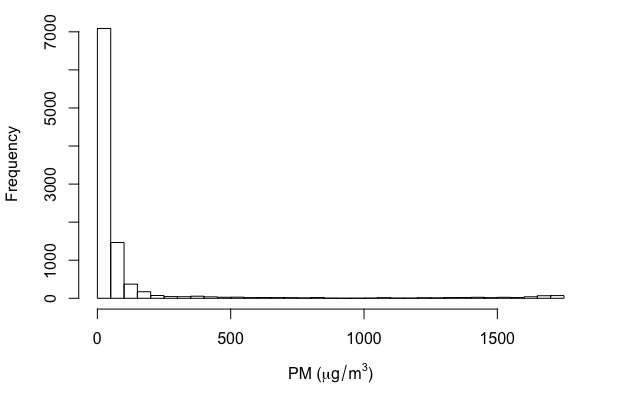
\includegraphics[width=\textwidth]{images/pm_histogram}
                \caption{Shinyei PPD42}
                \label{fig:pm_histogram}
            \end{subfigure}
            \hfill
            \begin{subfigure}[t]{.4\linewidth}
            	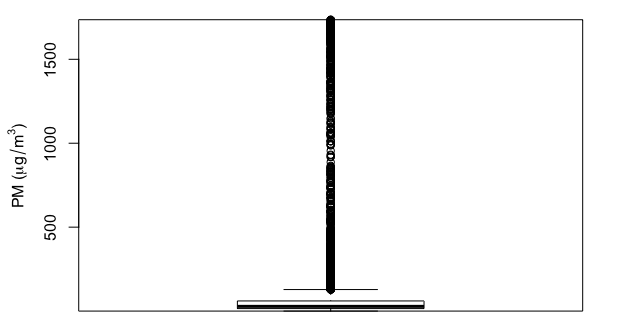
\includegraphics[width=\textwidth]{images/pm_boxplot}
            	\caption{Shinyei PPD42}
            	\label{fig:pm_boxplot}
	   \end{subfigure}
        \end{minipage}
    % MQ131
    \begin{minipage}{1\linewidth}
    \vspace{0pt}
            \begin{subfigure}[t]{.4\linewidth}
                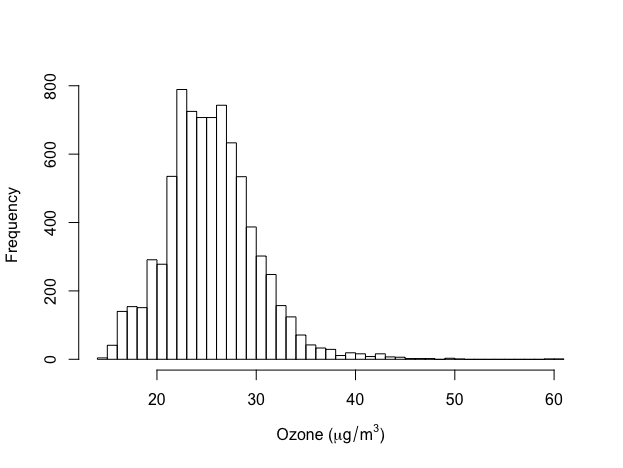
\includegraphics[width=\textwidth]{images/ozone_histogram}
                \caption{MQ131}
                \label{fig:ozone_histogram}
            \end{subfigure}
            \hfill
            \begin{subfigure}[t]{.4\linewidth}
            	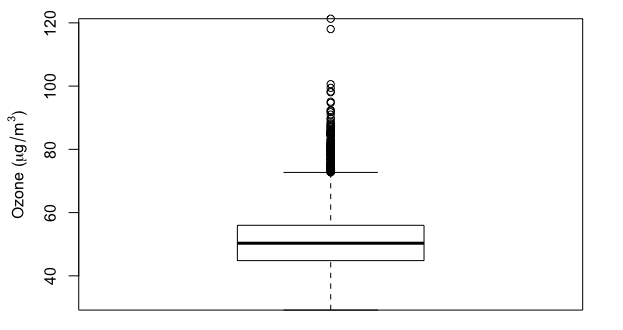
\includegraphics[width=\textwidth]{images/ozone_boxplot}
            	\caption{MQ131}
            	\label{fig:ozone_boxplot}
	   \end{subfigure}
        \end{minipage}
    % MQ135
    \begin{minipage}{1\linewidth}
            \begin{subfigure}[t]{.4\linewidth}
                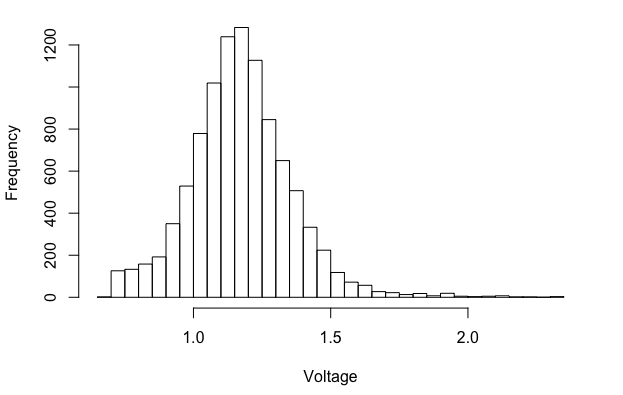
\includegraphics[width=\textwidth]{images/mq135_histogram}
                \caption{MQ135}
                \label{fig:mq135_histogram}
            \end{subfigure}
            \hfill
            \begin{subfigure}[t]{.4\linewidth}
            	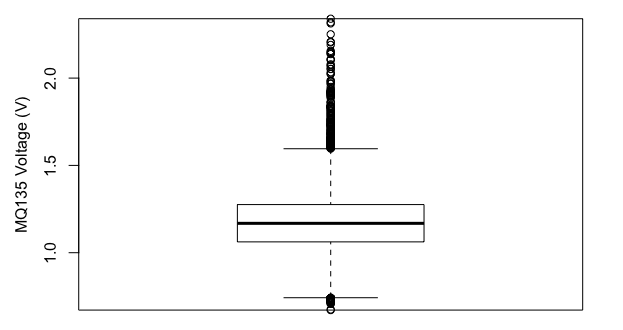
\includegraphics[width=\textwidth]{images/mq135_boxplot}
            	\caption{MQ135}
            	\label{fig:mq135_boxplot}
	   \end{subfigure}
        \end{minipage}
    % Temp
    \begin{minipage}{1\linewidth}
            \begin{subfigure}[t]{.4\linewidth}
                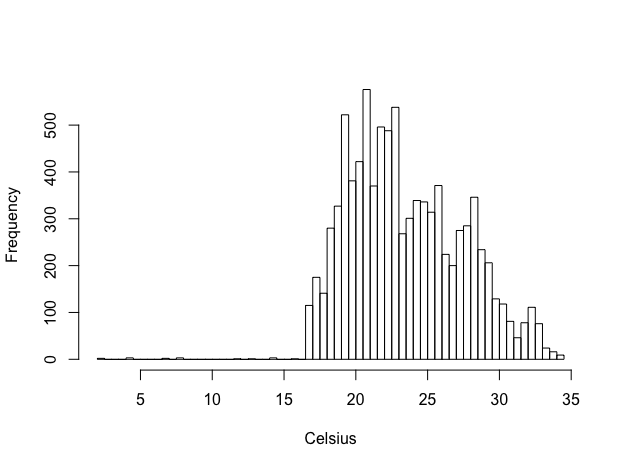
\includegraphics[width=\textwidth]{images/temp_histogram}
                \caption{DHT22 temperature}
                \label{fig:temp_histogram}
            \end{subfigure}
            \hfill
            \begin{subfigure}[t]{.4\linewidth}
            	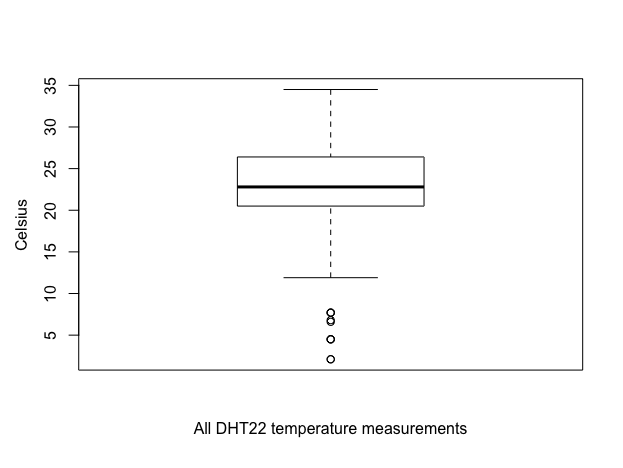
\includegraphics[width=\textwidth]{images/temp_boxplot}
            	\caption{DHT22 temperature}
            	\label{fig:temp_boxplot}
	   \end{subfigure}
        \end{minipage}
    % Humidity
    \begin{minipage}{1\linewidth}
            \begin{subfigure}[t]{.4\linewidth}
                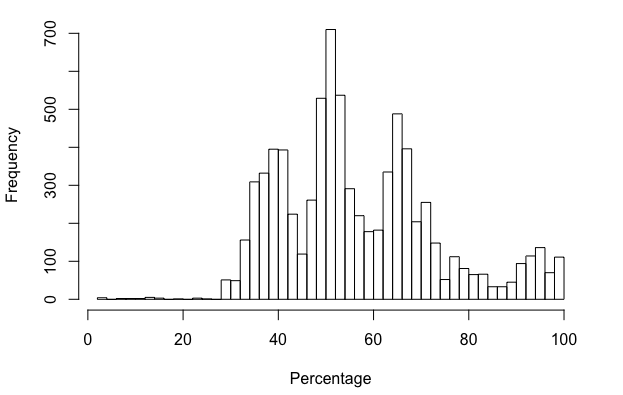
\includegraphics[width=\textwidth]{images/humidity_histogram}
                \caption{DHT22 humidity}
                \label{fig:humidity_histogram}
            \end{subfigure}
            \hfill
            \begin{subfigure}[t]{.4\linewidth}
            	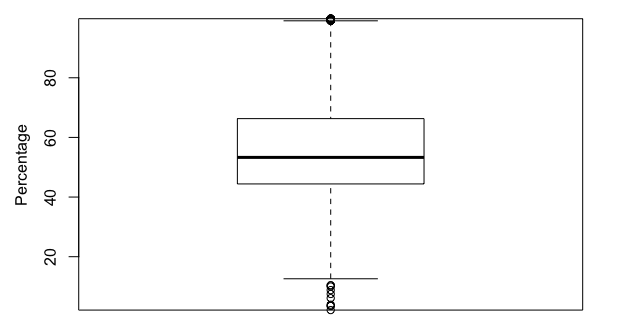
\includegraphics[width=\textwidth]{images/humidity_boxplot}
            	\caption{DHT22 humidity}
            	\label{fig:humidity_boxplot}
	   \end{subfigure}
        \end{minipage}
    \caption[Sensor measurement histograms and boxplots.]{Histograms and Tukey boxplots depicting the distribution of pollution sensor measurements.}
    \label{fig:histograms_and_boxplots}
\end{figure}

%\begin{figure}[!tbp]
%    \centering
%    \begin{minipage}{1\linewidth}
%            \begin{subfigure}[t]{.5\linewidth}
%                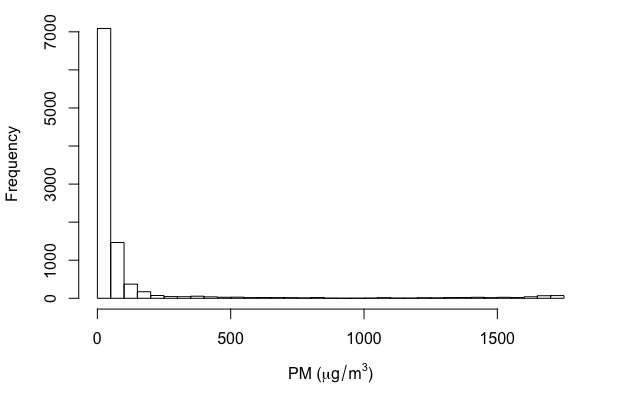
\includegraphics[width=\textwidth]{images/pm_histogram}
%                \caption{Shinyei PPD42}
%                \label{fig:pm_histogram}
%            \end{subfigure}
%            \begin{subfigure}[t]{.5\linewidth}
%            	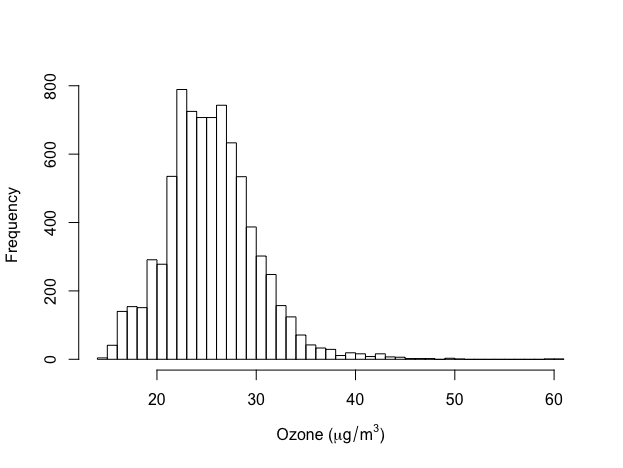
\includegraphics[width=\textwidth]{images/ozone_histogram}
%            	\caption{MQ131}
%            	\label{fig:ozone_histogram}
%	   \end{subfigure}
%        \end{minipage}
%    \begin{minipage}{1\linewidth}
%            \begin{subfigure}[t]{.5\linewidth}
%                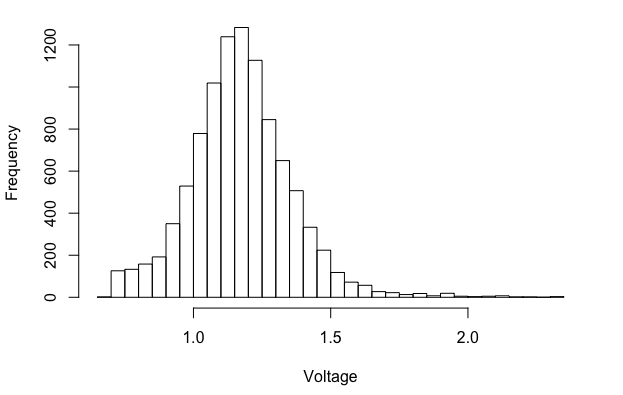
\includegraphics[width=\textwidth]{images/mq135_histogram}
%                \caption{MQ135}
%                \label{fig:mq135_histogram}
%            \end{subfigure}
%            \begin{subfigure}[t]{.5\linewidth}
%            	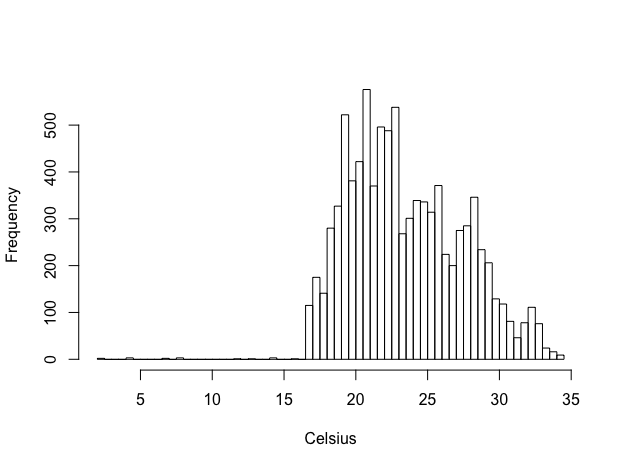
\includegraphics[width=\textwidth]{images/temp_histogram}
%            	\caption{DHT22 temperature}
%            	\label{fig:temp_histogram}
%	   \end{subfigure}
%        \end{minipage}
%    \begin{minipage}{1\linewidth}
%    	\centering
%        \begin{subfigure}[t]{.5\linewidth}
%            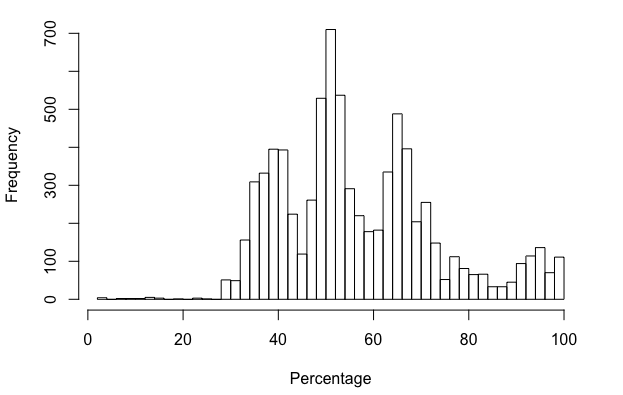
\includegraphics[width=\textwidth]{images/humidity_histogram}
%            \caption{DHT22 humidity}
%            \label{fig:humidity_histogram}
%        \end{subfigure}
%    \end{minipage}
%    \caption[Sensor measurement histograms.]{Histograms depicting the distribution of pollution sensor measurements. (a) shows a positive skew, with a number of extreme values; (b) and (c) have approximately normal distributions; (d) has a slight positive skew, with low frequencies of values below \SI{17}{\celsius}; (e) also has low frequency values below 25\% humidity, with a more varied distribution of values compared to the other histograms.}
%\end{figure}

As Figure \ref{fig:pm_histogram} shows, the distribution of PM10 measurements is positively skewed and it appears that the measurements contain a large number of outliers. The majority of the values are distributed between 0 and 200, with a number of other values spread out to over \num{1500}. Within the frequent observations, the positive skew indicates that lower measurements tend to be more common than higher measurements. Compared to the other histograms, the PM10 measurements from the Shinyei PPD42 particulate sensor have the largest range of values and, consequently, potentially the largest proportion of outliers.

Figures \ref{fig:ozone_histogram} and \ref{fig:mq135_histogram} show approximately normally distributed values from the MQ131 and MQ135 sensors, with some of the higher values potentially being outliers due to the long, thin tail on the right-hand side of the distribution.

The measurements from the DHT22 temperature and humidity sensor do not follow a normal distribution as closely. The temperature measurements (Figure \ref{fig:temp_histogram}) have a slight positive skew, with a range of low frequency values below \SI{17}{\celsius}. Likewise, the humidity measurements (Figure \ref{fig:humidity_histogram}) have a number of low frequency values below 25\% humidity, suggesting a number of outliers are present. These are noticeable by the sudden drop in frequency to the left-hand side of the distribution. Overall, the distribution of humidity measurements is more erratic, with a number of peaks in the distribution across a larger range.

%\begin{figure}[!htbp]
%    \centering
%    \begin{minipage}{1\linewidth}
%            \begin{subfigure}[t]{.5\linewidth}
%                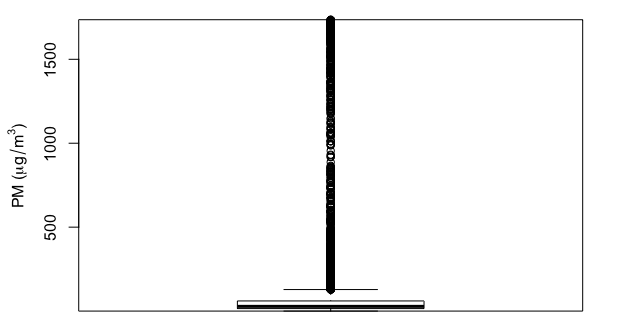
\includegraphics[width=\textwidth]{images/pm_boxplot}
%                \caption{Shinyei PPD42}
%                \label{fig:pm_boxplot}
%            \end{subfigure}
%            \begin{subfigure}[t]{.5\linewidth}
%            	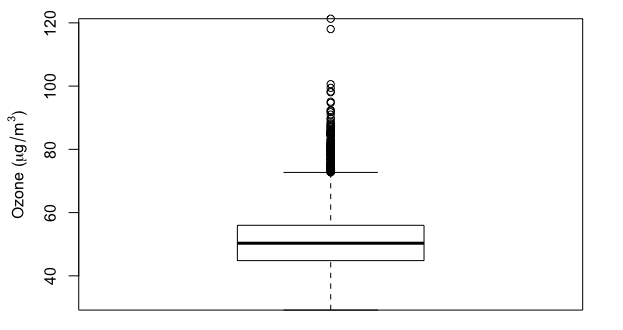
\includegraphics[width=\textwidth]{images/ozone_boxplot}
%            	\caption{MQ131}
%            	\label{fig:mq131_boxplot}
%	   \end{subfigure}
%        \end{minipage}
%    \begin{minipage}{1\linewidth}
%            \begin{subfigure}[t]{.5\linewidth}
%                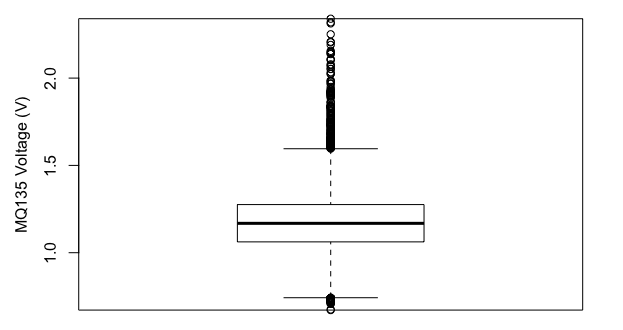
\includegraphics[width=\textwidth]{images/mq135_boxplot}
%                \caption{MQ135}
%                \label{fig:pm_boxplot}
%            \end{subfigure}
%            \begin{subfigure}[t]{.5\linewidth}
%            	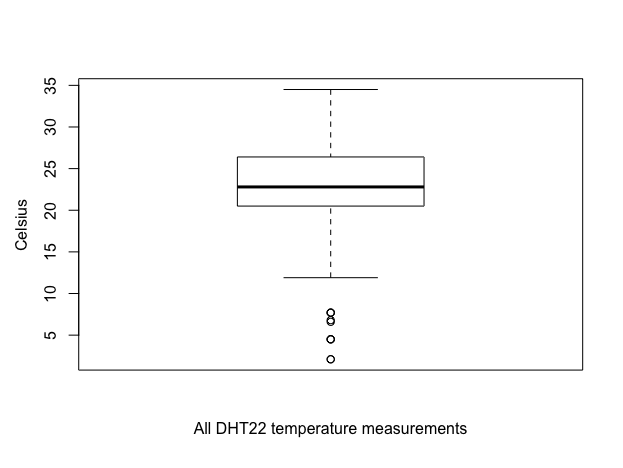
\includegraphics[width=\textwidth]{images/temp_boxplot}
%            	\caption{DHT22 temperature}
%            	\label{fig:temp_boxplot}
%	   \end{subfigure}
%        \end{minipage}
%    \begin{minipage}{1\linewidth}
%    	\centering
%        \begin{subfigure}[t]{.5\linewidth}
%            \includegraphics[width=\textwidth]{images/humidity_boxplot}
%            \caption{DHT22 humidity}
%            \label{fig:humidity_boxplot}
%        \end{subfigure}
%    \end{minipage}
%    \caption[Tukey's boxplots.]{Tukey's box-plot of sensor measurements. The `whiskers' represent the outlier boundaries. (a) displays a highly skewed distribution with a large number of outliers at the high-end of the distribution; (b) and (c) have similar distributions with a number of outliers at the high-end; (d) only has a small number of outliers at low values and is otherwise evenly distributed; (e) also has an even distribution with a small number of outliers at both high and low values.}
%    \label{tukey_boxplots}
%\end{figure}

\subsubsection{Outliers}

The process of identifying outliers in the data using each of the detection methods (IQR, MAD, S\textsubscript{n}) is extensive and including all the results here would be impractical. Instead, the more detailed results tables have been moved to Appendix \ref{appendix:outliers} and a general overview provided here.

Table \ref{tab:size_change} details the number of errors and outliers removed from the dataset, in both absolute and percentage terms. The first step of the data cleaning removes errors from the sensor measurements, which were measurements that were taken during periods of sensor malfunction. Up to 20\% of the measurements are excluded as a result. Next, measurements that are labelled as an outlier by all three methods are removed. It is clear from the table that the PM10 measurements have the highest percentage of outliers (11.3\%) compared to the other sensor measurements. For the other four sensors, the outlier percentages are between 1.0\% and 1.6\%, which are much lower and reasonable.

\begin{table}[!tbp]
  \centering
  \caption{Dataset size changes resulting from removing errors and outliers.}
  \label{tab:size_change}
  \begin{tabular}{ l S[table-format=5] S[table-format=5] S[table-format=4] S[table-format=2.1] S[table-format=5] S[table-format=4] S[table-format=2.1]}
  \toprule
   {} & {Initial} & \multicolumn{3}{c}{Errors removed} & \multicolumn{3}{c}{Outliers removed} \\
  \cmidrule(lr){2-2}
  \cmidrule(lr){3-5}
  \cmidrule(lr){6-8}
  Gas/particulate & \multicolumn{1}{c}{N} & \multicolumn{1}{c}{N} & \multicolumn{1}{c}{Diff.} & \multicolumn{1}{c}{\%} & \multicolumn{1}{c}{N} & \multicolumn{1}{c}{Diff.} & \multicolumn{1}{c}{\%}  \\ \midrule
  PM10			& 9877	& 9089	& 788	& 8.0		& 8063	& 1026	& 11.3 \\
  O\textsubscript{3}	& 9877	& 7920	& 1957	& 19.8	& 9837	& 83		& 1.0 \\
  General AQ		& 9877	& 9877	& 0		& 0.0		& 9737	& 140	& 1.4 \\ 
  Temperature		& 9877	& 9234	& 643	& 6.5		& 9132	& 102	& 1.1 \\ 
  Humidity			& 9877	& 7797 	& 2080	& 21.1	& 7672	& 125	& 1.6  \\ \bottomrule
 % Total			& 29631	& 26886	& 2745	& 9.3		& 26637	& 1249	& 4.6 \\ \bottomrule
  \end{tabular}
\end{table}

In addition, Table \ref{tab:upper_bounds} displays the upper bounds from running the outlier detection methods using different temporal groupings: on the dataset as a whole, by time period grouping (Week AM, Week PM, Weekend AM, Weekend PM) and moving average within each collection run. The upper bounds for all the sensors are lowest when using the dataset as a whole and highest when using moving averages, with per time period grouping in the middle. The maximum upper bound when using moving averages is abnormally high.

\begin{table}[!tbp]
  \centering
  \caption{Maximum upper bounds for each sensor, by temporal grouping method.}
  \label{tab:upper_bounds}
  \begin{tabular}{ l S[table-format=3.2] S[table-format=3.2] S[table-format=4.2] }
  \toprule
%   {} & {Initial} & \multicolumn{3}{c}{Errors removed} & \multicolumn{3}{c}{Outliers removed} \\
%  \cmidrule(lr){2-2}
%  \cmidrule(lr){3-5}
%  \cmidrule(lr){6-8}
  Gas/particulate & \multicolumn{1}{c}{Whole dataset} & \multicolumn{1}{c}{Time period grouping} & \multicolumn{1}{c}{Moving average} \\ \midrule
  PM10 ($\mu g/m^3$)			& 128.64	& 251.18	& 1768.13	 \\
  O\textsubscript{3} ($\mu g/m^3$)	& 75.69	& 91.59	& 146.23	 \\
  General AQ (V)				& 1.67	& 1.72	& 3.66		 \\
  Temperature (\SI{}{\celsius})		& 26.12	& 27.08	& 34.03 		  \\ 
  Humidity	(\%)					& 79.67	& 85.48	& 96.72	 	  \\ \bottomrule
  \end{tabular}
\end{table}


The use of moving averages when applying these methods results in too many measurements being identified as outliers -- many of these would otherwise not be considered outliers if the methods were run on the dataset as a whole. It is still beneficial to separate the dataset into time period groupings, however, in order to account for temporal variation. 

The results indicate that moving averages should definitely not be used, which leaves the other two options remaining. We choose to use per time period grouping because, although the maximum upper bounds are slightly higher, it takes into account temporal variation.

Therefore, the methods are run per time period grouping. For a value to be considered an outlier, all of the three methods -- IQR, MAD and S\textsubscript{n} -- have to identify it as an outlier. These values are then filtered out. Histograms of the pollution measurements from the cleaned dataset are shown in Figure \ref{fig:histograms_clean}. The resulting changes in dataset sizes, from the initial dataset to the final dataset with outliers removed, are shown in Table \ref{tab:size_change}.

\begin{figure}[!tbp]
    \centering
    \begin{minipage}{1\linewidth}
            \begin{subfigure}[t]{.5\linewidth}
                \includegraphics[width=\textwidth]{images/pm_histogram_clean}
                \caption{Shinyei PPD42}
                \label{fig:pm_histogram_clean}
            \end{subfigure}
            \begin{subfigure}[t]{.5\linewidth}
            	\includegraphics[width=\textwidth]{images/ozone_histogram_clean}
            	\caption{MQ131}
            	\label{fig:ozone_histogram_clean}
	   \end{subfigure}
        \end{minipage}
    \begin{minipage}{1\linewidth}
            \begin{subfigure}[t]{.5\linewidth}
                \includegraphics[width=\textwidth]{images/mq135_histogram_clean}
                \caption{MQ135}
                \label{fig:mq135_histogram_clean}
            \end{subfigure}
            \begin{subfigure}[t]{.5\linewidth}
            	\includegraphics[width=\textwidth]{images/histogram_temp_clean}
            	\caption{DHT22 temperature}
            	\label{fig:temp_histogram_clean}
	   \end{subfigure}
        \end{minipage}
    \begin{minipage}{1\linewidth}
    	\centering
        \begin{subfigure}[t]{.5\linewidth}
            \includegraphics[width=\textwidth]{images/histogram_humidity_clean}
            \caption{DHT22 humidity}
            \label{fig:humidity_histogram_clean}
        \end{subfigure}
    \end{minipage}
    \caption[Sensor measurement histograms with cleaned data.]{Histograms depicting the distribution of pollution sensor measurements with cleaned data. (a) shows a slight positive skew, (b), (c) and (d) have approximately normal distributions, and (e) has a more varied distribution.}
    \label{fig:histograms_clean}
\end{figure}

%\subsubsection{Outlier detection methods}
%
%The first method for detecting outliers, as detailed in Section \ref{iqr}, uses the IQR. The IQR is visualised in Tukey's boxplot by the height of the box -- the top indicates the 75th quartile and the bottom indicates the 25th quartile. Figure \ref{fig:histograms_and_boxplots} shows the boxplots for each of the sensors. These show that all of the sensor measurements have a non-zero number of outliers, although the Shinyei PPD42, MQ131 and MQ135 sensors appear to have the most, indicated by the number of points outside of the `whiskers' of the boxplots. These whiskers represent the outlier detection rule of 1.5 times the IQR away from the 25th and 75th quartiles.
%
%The results of performing this outlier detection method are shown in Table \ref{tab:iqr_outliers}. It is clear from the table that the PM10 measurements have the highest percentage of outliers (11.75\%) compared to the ozone (1.79\%) and general air quality measurements (1.97\%). The upper bound of 128.64 $\mu g/m^3$ is reasonable, given that the highest PM10 measurement recorded in 2017 by the Windsor Bridge monitoring station in Bath was 204 $\mu g/m^3$ \citep{courthold2018max}. The MQ131 sensor has the lowest percentage of outliers when using the IQR detection method. It must be noted that the sample size $N$ for the ozone measurements is considerably lower than for the other two pollutants due to the aforementioned breakage and replacement of the MQ131 sensor midway through data collection. However, the percentage of outliers is similar to that for the general air quality measurements, so this exclusion does not appear to have detrimentally impacted the analysis from a statistical perspective.
%
%The second outlier detection method is the median and MAD method. Outliers were identified as any measurements which were more than 3 times the MAD away from the median. The results of this method are detailed in Table \ref{tab:mad_outliers}. Once again, PM10 shows the highest percentage of outliers, with 14.14\% of the measurements being considered outliers. This is a 2.39\% increase over the number of outliers found by the IQR detection method. On the other hand, there has been a small decrease in the outlier percentages for the ozone and general air quality measurements. However, overall, the values are not too dissimilar to those found by the IQR method, which indicates the robustness of these methods.
%
%The third method uses the median and S\textsubscript{n} and the results are shown in Table \ref{tab:mad_outliers}. The PM10 outlier percentage is only 0.07\% less than using the MAD method. The percentage of outliers for ozone and general air quality are the lowest out of the three methods.
%
%
%\begin{table}[!tbp]
%  \centering
%  \caption{Outlier detection summary using IQR method on the whole dataset.}
%  \label{tab:iqr_outliers}
%  \begin{tabular}{ l l S[table-format=3.2] S[table-format=3.2] S[table-format=3.2] S[table-format=3.2] S[table-format=3.2] S[table-format=3.2] }
%  \toprule
%  Gas/particulate & N & {Median} & {IQR} & {U.B.} & {L.B.*} & {\# outliers} & {\%} \\ \midrule
%  PM10 $(\mu g/m^3)$ & 9089 & 28.13 & 45.50 & 128.64 & 0.00 & 1068 & 11.75 \\
%  O\textsubscript{3} $(\mu g/m^3)$ & 7920 & 50.31 & 11.17 & 72.74 & 28.06 & 142 & 1.79 \\
%  General AQ (V) & 9877 & 1.17 & 0.21 & 1.60 & 0.74 & 195 & 1.97 \\ \bottomrule
%    \multicolumn{7}{l}{\textsuperscript{$\ast$}\footnotesize{Lower bound (L.B.) capped at 0 as negative concentrations are nonsensical.}} \\
%  \end{tabular}
%\end{table}
%% Include temp and humidity as well?
%
%%\subsubsection{Median and MAD}
%%
%%The median and MAD outlier detection method was also implemented. Outliers were identified as any measurements which were more than 3 times the MAD away from the median.
%%
%%The results of this method are detailed in Table \ref{tab:mad_outliers}. Once again, PM10 shows the highest percentage of outliers, with 14.14\% of the measurements being considered outliers. This is a 2.39\% increase over the number of outliers found by the IQR detection method. On the other hand, there has been a small decrease in the outlier percentages for the ozone and general air quality measurements. However, overall, the values are not too dissimilar to those found by the IQR method, which indicates the robustness of these methods.
%
%\begin{table}[!tbp]
%  \centering
%  \caption{Outlier detection summary using median and MAD method on the whole dataset.}
%  \label{tab:mad_outliers}
%  \begin{tabular}{ l l S[table-format=3.2] S[table-format=3.2] S[table-format=3.2] S[table-format=3.2] S[table-format=3.2] S[table-format=3.2] }
%  \toprule
%  Gas/particulate & N & {Median} & {MAD} & {U.B.} & {L.B.*} & {\# outliers} & {\%} \\ \midrule
%  PM10 $(\mu g/m^3)$ & 9089 & 28.13 & 25.38 & 104.26 & 0.00 & 1285 & 14.14 \\
%  O\textsubscript{3} $(\mu g/m^3)$ & 7920 & 50.31 & 8.30 & 75.21 & 25.42 & 105 & 1.33 \\
%  General AQ (V) & 9877 & 1.17 & 0.16 & 1.65 & 0.69 & 139 & 1.41 \\ \bottomrule
%    \multicolumn{7}{l}{\textsuperscript{$\ast$}\footnotesize{Lower bound (L.B.) capped at 0 as negative concentrations are nonsensical.}} \\
%  \end{tabular}
%\end{table}
%
%%\subsubsection{S\textsubscript{n}}
%%
%%Table \ref{tab:mad_outliers} shows the result of the S\textsubscript{n} method of outlier detection. The PM10 outlier percentage is only 0.07\% less than using the MAD method. The percentage of outliers for ozone and general air quality are the lowest out of the three methods.
%
%\begin{table}[!tbp]
%  \centering
%  \caption{Outlier detection summary using median and S\textsubscript{n} method on the whole dataset.}
%  \label{tab:mad_outliers}
%  \begin{tabular}{ l l S[table-format=3.2] S[table-format=3.2] S[table-format=3.2] S[table-format=3.2] S[table-format=3.2] S[table-format=3.2] }
%  \toprule
%  Gas/particulate & N & {Median} & {S\textsubscript{n}} & {U.B.} & {L.B.*} & {\# outliers} & {\%} \\ \midrule
%  PM10 $(\mu g/m^3)$ & 9089 & 28.13 & 25.22 & 103.80 & 0.00 & 1288 & 14.17 \\
%  O\textsubscript{3} $(\mu g/m^3)$ & 7920 & 50.31 & 8.46 & 75.69 & 24.94 & 97 & 1.22 \\
%  General AQ (V) & 9877 & 1.17 & 0.17 & 1.67 & 0.67 & 121 & 1.23 \\ \bottomrule
%    \multicolumn{7}{l}{\textsuperscript{$\ast$}\footnotesize{Lower bound (L.B.) capped at 0 as negative concentrations are nonsensical.}} \\
%  \end{tabular}
%\end{table}
%
%\subsubsection{Per time period group}
%
%The above methods are also implemented on a per-group basis, with the group being the week period (Week AM, Week PM, Weekend AM, Weekend PM). These results are shown in column 2 of Table \ref{tab:all_outliers}. In the interest of clarity, the table is simplified to only show the main figures. The results show that, on average, running the outlier detection on a per-group basis leads to a slightly decreased number of measurements identified as outliers. Although the number of outliers rises when using the MAD and S\textsubscript{n} methods, the number of outliers detected by using the IQR method actually falls. It is also clear that PM10 has the highest number of outliers. When running these methods on the sample as a whole, the MAD method leads to the highest total number of outliers, but this changes to the S\textsubscript{n} when running the methods per time period grouping.
%
%\subsubsection{Moving average}
%
%The outlier detection methods are also applied using moving averages, to account for the time series nature of the data. The results are shown in column 3 of Table \ref{tab:all_outliers}. The results show that the number of outliers for PM10 reduces considerably, but the figure increases for O\textsubscript{3} and General AQ measurements, with the number of outliers increasing by approximately a factor of 3.
%
%\begin{landscape}
%\begin{table}[!tbp]
%  \centering
%  \small
%  \caption{Total number of outliers when running each method on the whole sample or per time period grouping. On average, per time period grouping leads to a higher number of measurements being identified as outliers.}
%  \label{tab:all_outliers}
%  \begin{tabular}{ l S[table-format=4] S[table-format=4] S[table-format=4] S[table-format=4] S[table-format=4] S[table-format=4] S[table-format=4] S[table-format=4] S[table-format=4] S[table-format=4] S[table-format=4] S[table-format=4] }
%  \toprule
%  {} & \multicolumn{4}{c}{Whole dataset} & \multicolumn{4}{c}{Time period grouping} & \multicolumn{4}{c}{Moving average} \\
%  \cmidrule(lr){2-5}
%  \cmidrule(lr){6-9}
%  \cmidrule(lr){10-13}
%  Gas/particulate & \multicolumn{1}{l}{IQR} & \multicolumn{1}{l}{MAD} & \multicolumn{1}{l}{S\textsubscript{n}} & \multicolumn{1}{l}{Avg.} & \multicolumn{1}{l}{IQR} & \multicolumn{1}{l}{MAD} & \multicolumn{1}{l}{S\textsubscript{n}} & \multicolumn{1}{l}{Avg.} & \multicolumn{1}{l}{IQR} & \multicolumn{1}{l}{MAD} & \multicolumn{1}{l}{S\textsubscript{n}} & \multicolumn{1}{l}{Avg.} \\ \midrule
%  PM10			& 1068	& 1285	& 1288	& 1214	& 1026	& 1298	& 1304	& 1209	& 980	& 800	& 769	& 850	\\
%  O\textsubscript{3}	& 142	& 105	& 97		& 115	& 136	& 89		& 93		& 106	& 612	& 502	& 463	& 526	\\
%  General AQ		& 195	& 139	& 121	& 152	& 201	& 152	& 141	& 165 	& 674	& 406	& 342	& 474	\\ \midrule
%  Total			& 1405	& 1529	& 1506	& 1480	& 1363	& 1539	& 1538	& 1480	& 2266	& 1708	& 1574	& 1850	\\ \bottomrule
%  \end{tabular}
%\end{table}
%\end{landscape}

%\subsubsection{Geo-spatial outliers}
%
%There were a small number of geo-spatial outliers, which were corrected using the method detailed in Section \ref{gps_outliers}.
%% Might need to edit to remove reference to event-based collection period
%Since the routes in each of the three data collection periods are consistent, the longitude and latitude measurements create waveform-like patterns. These are useful in identifying outliers as they clearly show when the value exceeds the usual minimums and maximums (represented by red horizontal lines). For example, Figure \ref{fig:waves} shows the longitude and latitude time series from the event-based collection period. Figure \ref{fig:wave_longitudes} has erratic longitude measurements until 18:45, before settling into a consistent pattern. Figure \ref{fig:wave_latitudes} has a slightly longer period of inconsistent latitude measurements and the values are clearly erroneous as they stretch far away from the peaks of the pattern.
%
%\begin{figure}[!tb]
%    \centering
%    \begin{minipage}{1\linewidth}
%            \begin{subfigure}[t]{.5\linewidth}
%                \includegraphics[width=\textwidth]{images/wave_longitudes}
%                \caption{Longitudes}
%                \label{fig:wave_longitudes}
%            \end{subfigure}
%            \begin{subfigure}[t]{.5\linewidth}
%            	\includegraphics[width=\textwidth]{images/wave_latitudes}
%            	\caption{Latitudes}
%            	\label{fig:wave_latitudes}
%	   \end{subfigure}
%        \end{minipage}
%    \caption[Longitude and latitude waveforms.]{Longitude and latitude data from a consistent route creates a waveform, which can be used to identify outliers. Values outside of the pattern's minimum and maximum (shown by the horizontal red lines) or that appear irregular can be considered outliers.}
%    \label{fig:waves}
%\end{figure}
%
%\subsubsection{Outlier summary}
%
%The use of moving averages when applying these methods results in too many measurements being identified as outliers -- many of these would otherwise not be considered outliers if the methods were run on the dataset as a whole. It is still beneficial to separate the dataset into time period groupings, however, in order to account for temporal variation. Therefore, the methods are run per time period grouping. For a value to be considered an outlier, all of the three methods -- IQR, MAD and S\textsubscript{n} -- have to identify it as an outlier. These values are then filtered out. Histograms of the pollution measurements from the cleaned dataset are shown in Figure \ref{fig:histograms_clean}. The resulting changes in dataset sizes, from the initial dataset to the final dataset with outliers removed, are shown in Table \ref{tab:size_change}.
%
%\begin{figure}[!tbp]
%    \centering
%    \begin{minipage}{1\linewidth}
%            \begin{subfigure}[t]{.5\linewidth}
%                \includegraphics[width=\textwidth]{images/pm_histogram_clean}
%                \caption{Shinyei PPD42}
%                \label{fig:pm_histogram_clean}
%            \end{subfigure}
%            \begin{subfigure}[t]{.5\linewidth}
%            	\includegraphics[width=\textwidth]{images/ozone_histogram_clean}
%            	\caption{MQ131}
%            	\label{fig:ozone_histogram_clean}
%	   \end{subfigure}
%        \end{minipage}
%    \begin{minipage}{1\linewidth}
%            \begin{subfigure}[t]{.5\linewidth}
%                \includegraphics[width=\textwidth]{images/mq135_histogram_clean}
%                \caption{MQ135}
%                \label{fig:mq135_histogram_clean}
%            \end{subfigure}
%            \begin{subfigure}[t]{.5\linewidth}
%            	\includegraphics[width=\textwidth]{images/histogram_temp_clean}
%            	\caption{DHT22 temperature}
%            	\label{fig:temp_histogram_clean}
%	   \end{subfigure}
%        \end{minipage}
%    \begin{minipage}{1\linewidth}
%    	\centering
%        \begin{subfigure}[t]{.5\linewidth}
%            \includegraphics[width=\textwidth]{images/histogram_humidity_clean}
%            \caption{DHT22 humidity}
%            \label{fig:humidity_histogram_clean}
%        \end{subfigure}
%    \end{minipage}
%    \caption[Sensor measurement histograms with cleaned data.]{Histograms depicting the distribution of pollution sensor measurements with cleaned data. (a) shows a slight positive skew, (b), (c) and (d) have approximately normal distributions, and (e) has a more varied distribution.}
%    \label{fig:histograms_clean}
%\end{figure}

%\begin{table}[!tbp]
%  \centering
%  \caption{Dataset size changes.}
%  \label{tab:size_change}
%  \begin{tabular}{ l S[table-format=5] S[table-format=5] S[table-format=4] S[table-format=2.1] S[table-format=5] S[table-format=4] S[table-format=2.1]}
%  \toprule
%   {} & {Initial} & \multicolumn{3}{c}{Errors removed} & \multicolumn{3}{c}{Outliers removed} \\
%  \cmidrule(lr){2-2}
%  \cmidrule(lr){3-5}
%  \cmidrule(lr){6-8}
%  Gas/particulate & \multicolumn{1}{c}{N} & \multicolumn{1}{c}{N} & \multicolumn{1}{c}{Diff.} & \multicolumn{1}{c}{\%} & \multicolumn{1}{c}{N} & \multicolumn{1}{c}{Diff.} & \multicolumn{1}{c}{\%}  \\ \midrule
%  PM10			& 9877	& 9089	& 788	& 8.0		& 8063	& 1026	& 11.3 \\
%  O\textsubscript{3}	& 9877	& 7920	& 1957	& 19.8	& 9837	& 83		& 1.0 \\
%  General AQ		& 9877	& 9877	& 0		& 0.0		& 9737	& 140	& 1.4 \\ \midrule
%  Total			& 29631	& 26886	& 2745	& 9.3		& 26637	& 1249	& 4.6 \\ \bottomrule
%  \end{tabular}
%\end{table}

%Regarding the geo-spatial outliers, these have been corrected as best possible. Where they still remain erroneous, these measurements have been discarded from any geo-spatial analysis. However, the geo-spatial measurement being an outlier does not affect the pollution sensor measurements, so these remain for the other analyses.


\subsection{Maps}
% High resolution maps
% Hotspots?
% Land-use regression (LUR) modelling ?

Using the cleaned dataset, pollution levels along the route can be mapped. Figure \ref{fig:route_pollution_maps} shows pollution maps for each of the pollutants. Each pollutant has two maps: the first uses the mean of all measurements inside each tile's boundaries to colour the tile and the second uses the maximum. By analysing the colours of the tiles in these maps, it is possible to identify high pollution areas in Bath.

Figure \ref{fig:pm10_map_median} shows some variation in PM10 levels around the route, with the majority varying between 20-50~$\mu g/m^3$. In addition, there are a small number of highly elevated PM10 levels, one of which is found in the north west corner of the route at a level of 100~$\mu g/m^3$ (Long = -2.378, Lat = 51.386). This location is directly outside the waste recycling facility in Bath, which may be the source of the pollution. By using the maximum aggregation instead, Figure \ref{fig:pm10_map_max} shows that large sections of the route have measured a high level of pollution at some point during the data collection period. The average ozone levels along the route are shown in Figure \ref{fig:o3_map_median}, which indicates that the worst O\textsubscript{3} pollution is along the road in the south west part of the route (Long = -2.382 to -2.364, Lat = 51.377 to 51.382). This road is Lower Bristol Road and is one of the busiest roads in Bath because it leads to the A36 (a major road). The median ozone pollution level appears to be in the 50-60~$\mu g/m^3$ range. The maximum pollution levels (Figure \ref{fig:o3_map_max}) are elevated along the whole route compared to the median levels, which is as expected. Overall, there is little variation in the maximum pollution levels around the route. The only noticeable maximum in solid red is again in the north west of the route, on the north side of Windsor Bridge (Long = -2.382, Lat = 51.385). This is located at one of the larger traffic junctions in Bath and is situated nearby the aforementioned waste recycling centre, both of which could be contributing to this higher reading. Again, the median general air quality (Figure \ref{fig:mq135_map_median}) does not vary dramatically, with a small number of highly elevated levels sparsely distributed around the route. These problem areas appear to be outside of an old storage warehouse demolition site (Long = -2.367, Lat = 51.378) and at a large traffic junction on London Road (Long = -2.358, Lat = 51.390). Using the maximum to aggregate each tiles' values, the majority of the route has experienced a high measurement from the general air quality sensor, with no particular area being better than others.

\begin{figure}[!htbp]
    \centering
    \begin{minipage}{1\linewidth}
            \begin{subfigure}[t]{.5\linewidth}
                \includegraphics[width=\textwidth]{images/pm10_map_median}
                \caption{PM10 (median)}
                \label{fig:pm10_map_median}
            \end{subfigure}
            \begin{subfigure}[t]{.5\linewidth}
            	\includegraphics[width=\textwidth]{images/pm10_map_max}
            	\caption{PM10 (max)}
            	\label{fig:pm10_map_max}
	   \end{subfigure}
        \end{minipage}
    \begin{minipage}{1\linewidth}
            \begin{subfigure}[t]{.5\linewidth}
                \includegraphics[width=\textwidth]{images/o3_map_median}
                \caption{O\textsubscript{3} (median)}
                \label{fig:o3_map_median}
            \end{subfigure}
            \begin{subfigure}[t]{.5\linewidth}
            	\includegraphics[width=\textwidth]{images/o3_map_max}
            	\caption{O\textsubscript{3} (max)}
            	\label{fig:o3_map_max}
	   \end{subfigure}
        \end{minipage}
    \begin{minipage}{1\linewidth}
            \begin{subfigure}[t]{.5\linewidth}
                \includegraphics[width=\textwidth]{images/mq135_map_median}
                \caption{General AQ (median)}
                \label{fig:mq135_map_median}
            \end{subfigure}
            \begin{subfigure}[t]{.5\linewidth}
            	\includegraphics[width=\textwidth]{images/mq135_map_max}
            	\caption{General AQ (max)}
            	\label{fig:mq135_map_max}
	   \end{subfigure}
        \end{minipage}
    \caption[Air quality pollution maps of the route.]{Air quality pollution maps of the route. The maps are separated vertically by the type of pollutant, with the LHS showing the median values and the RHS showing the maximum values.}
    \label{fig:route_pollution_maps}
\end{figure}


\subsection{Pattern analysis}
% Any differences between days of week?
% Week vs weekend
% Morning vs afternoon
% Direction of travel

The pollution maps display how the results vary spatially. We now present how the results differ temporally and in relation to other factors (speed of the bicycle, altitude, temperature and humidity). Any such patterns that can be identified in the data collected by the air quality monitoring device are displayed.

\subsubsection{Day of the week}

Figure \ref{fig:dow_bars} shows the median pollution levels for each pollutant by the day of the week. As Figure \ref{fig:dow_pm10} shows, the average pollution level increases throughout the week, from a low on Monday of 20$\mu g/m^3$ to a high on Sunday of over 30 $\mu g/m^3$. There is no identifiable pattern in Figure \ref{fig:dow_o3} for O\textsubscript{3} or Figure \ref{fig:dow_mq135} for general air quality.

\begin{figure}[!tbp]
    \centering
    \minipage{0.33\textwidth}
      \includegraphics[width=\linewidth]{images/dow_pm10}
      \caption{PM10}
      \label{fig:dow_pm10}
    \endminipage\hfill
    \minipage{0.33\textwidth}
      \includegraphics[width=\linewidth]{images/dow_o3}
      \caption{O\textsubscript{3}}
      \label{fig:dow_o3}
    \endminipage\hfill
    \minipage{0.33\textwidth}
      \includegraphics[width=\linewidth]{images/dow_mq135}
      \caption{MQ135}
      \label{fig:dow_mq135}
    \endminipage
    \caption[Pollution by day of the week.]{Pollution by day of the week. Each bar represents the median pollution level for that day.}
    \label{fig:dow_bars}
\end{figure}

%\begin{figure}[!htbp]
%    \centering
%    \begin{minipage}{1\linewidth}
%            \begin{subfigure}[t]{.45\linewidth}
%                \includegraphics[width=\textwidth]{images/dow_pm10}
%                \caption{PM10}
%                \label{fig:dow_pm10}
%            \end{subfigure}
%            \begin{subfigure}[t]{.45\linewidth}
%            	\includegraphics[width=\textwidth]{images/dow_o3}
%            	\caption{O\textsubscript{3}}
%            	\label{fig:dow_o3}
%	   \end{subfigure}
%        \end{minipage}
%    \begin{minipage}{1\linewidth}
%    	\centering
%            \begin{subfigure}[t]{.45\linewidth}
%                \includegraphics[width=\textwidth]{images/dow_mq135}
%                \caption{General AQ}
%                \label{fig:dow_mq135}
%            \end{subfigure}
%        \end{minipage}
%    \caption[Pollution by day of the week.]{Pollution by day of the week. Each bar represents the median pollution level for that day. (a) shows PM10, (b) shows O\textsubscript{3}, and (c) shows general air quality.}
%    \label{fig:dow_bars}
%\end{figure}

\subsubsection{Morning vs. Evening}

\begin{figure}[!htbp]
    \centering
    \minipage{0.33\textwidth}
      \includegraphics[width=\linewidth]{images/week_period_pm10}
      \caption{PM10}
      \label{fig:week_period_pm10}
    \endminipage\hfill
    \minipage{0.33\textwidth}
      \includegraphics[width=\linewidth]{images/week_period_o3}
      \caption{O\textsubscript{3}}
      \label{fig:week_period_o3}
    \endminipage\hfill
    \minipage{0.33\textwidth}
      \includegraphics[width=\linewidth]{images/week_period_mq135}
      \caption{MQ135}
      \label{fig:week_period_mq135}
    \endminipage
    \caption[Pollution by AM/PM and period of the week.]{Pollution by AM/PM and period of the week. Each bar represents the median pollution level for that time period.}
    \label{fig:week_period_bars}
\end{figure}

Figure \ref{fig:week_period_bars} shows the median pollution levels for each pollutant by AM/PM and the week period (week/weekend), as initially detailed in Section \ref{time_series_incorp}. For PM10, the measurements from the morning collection runs (AM) are on average higher than the measurements from the evening collection runs (PM). This holds for both the week and weekend periods. Similarly, this relationship also occurs with the O\textsubscript{3} measurements, although the difference is very slight with the week period. However, this relationship does not completely hold for the general air quality measurements since the weekend PM period has a higher average compared to the weekend AM period.

%\begin{figure}[!tb]
%    \centering
%    \begin{minipage}{1\linewidth}
%            \begin{subfigure}[t]{.45\linewidth}
%                \includegraphics[width=\textwidth]{images/week_period_pm10}
%                \caption{PM10}
%                \label{fig:week_period_pm10}
%            \end{subfigure}
%            \begin{subfigure}[t]{.45\linewidth}
%            	\includegraphics[width=\textwidth]{images/week_period_o3}
%            	\caption{O\textsubscript{3}}
%            	\label{fig:week_period_o3}
%	   \end{subfigure}
%        \end{minipage}
%    \begin{minipage}{1\linewidth}
%    	\centering
%            \begin{subfigure}[t]{.45\linewidth}
%                \includegraphics[width=\textwidth]{images/week_period_mq135}
%                \caption{General AQ}
%                \label{fig:week_period_mq135}
%            \end{subfigure}
%        \end{minipage}
%    \caption[Pollution by AM/PM and period of the week.]{Pollution by AM/PM and period of the week. Each bar represents the median pollution level for that time period.}
%    \label{fig:week_period_bars}
%\end{figure}


% Morning vs Evening maps as well

\subsubsection{Road}

\begin{figure}[!tb]
\centering
\includegraphics[width=0.6\textwidth]{images/road_pm}
\caption[Boxplot by road.]{Boxplot by road.}
\label{fig:road_pm}
\end{figure}


\subsubsection{Traffic}

\begin{table}[!tb]
\centering
\caption{Summary of road sections and corresponding traffic counts. AADF = Annual Average Daily Flow for all motor vehicles.}
\label{tab:speed}
\begin{tabular}{l c S[table-format=5]}
\toprule
Section name & Code & \multicolumn{1}{c}{AADF} \\ 
\midrule
Lower Bristol Road & LB & 23173 \\
Windsor Bridge & WB & 18269 \\
Upper Bristol Road & UB & 16978 \\
Queen's Square & QS & 8056 \\
The Paragon & TP & 8583 \\
London Road & LR & 23173 \\
Bathwick Street & BS & 15824 \\
Great Pulteney Street & GPS & 3267 \\
Manvers Street & MS & 5489 \\
Dorchester Street & DS & 7051 \\
\bottomrule
\end{tabular}
\end{table}

\subsubsection{Speed of the bicycle}

Figure \ref{fig:speed} shows the effect of the bicycle's speed on the sensor measurements. This is accompanied by a regression table in Table \ref{tab:speed}, which details the results of regressing each pollutant's measurements on corresponding speed measurements. A higher speed is associated with a higher PM10 reading. More specifically, every additional 1~m/s increase in speed leads to a 1.31~$\mu g/m^3$ increase in PM10 pollution, on average. On the other hand, a higher speed is associated with a lower O\textsubscript{3} reading, with a coefficient of -0.30~$\mu g/m^3$. Similarly, the general air quality measurement decreases by an average of 0.007~V for a unit increase in speed. These three findings are all statistically significant at the 1\% level. Overall, there is a wide dispersion of measurements for each of the sensors, which leads to low R\textsuperscript{2} values.

\begin{figure}[!tb]
    \centering
    \begin{minipage}{1\linewidth}
            \begin{subfigure}[t]{.32\linewidth}
                \includegraphics[width=\textwidth]{images/speed_pm}
                \caption{PM10}
                \label{fig:speed_pm10}
            \end{subfigure}
            \begin{subfigure}[t]{.32\linewidth}
            	\includegraphics[width=\textwidth]{images/speed_o3}
            	\caption{O\textsubscript{3}}
            	\label{fig:speed_o3}
	        \end{subfigure}
            \begin{subfigure}[t]{.32\linewidth}
                \includegraphics[width=\textwidth]{images/speed_mq135}
                \caption{General AQ}
                \label{fig:speed_mq135}
            \end{subfigure}
        \end{minipage}
    \caption[Relationship between speed and sensor measurements.]{Relationship between speed and sensor measurements.}
    \label{fig:speed}
\end{figure}

%\begin{figure}[!tb]
%    \centering
%    \minipage{0.33\textwidth}
%      \includegraphics[width=\linewidth]{images/speed_pm}
%      \caption{PM10}
%      \label{fig:speed_pm}
%    \endminipage\hfill
%    \minipage{0.33\textwidth}
%      \includegraphics[width=\linewidth]{images/speed_o3}
%      \caption{O\textsubscript{3}}
%      \label{fig:speed_o3}
%    \endminipage\hfill
%    \minipage{0.33\textwidth}
%      \includegraphics[width=\linewidth]{images/speed_mq135}
%      \caption{MQ135}
%      \label{fig:speed_mq135}
%    \endminipage
%    \caption[Effect of speed on sensor measurements.]{Effect of speed on sensor measurements.}
%    \label{fig:speed}
%\end{figure}

\begin{table}[!tb]
\centering
\caption{Effect of speed on pollution measurements.}
\label{tab:speed}
\begin{tabular}{c c c c}
\toprule
Variable & PM10 & Ozone & General AQ \\ 
\midrule
speed	& 1.305***		& -0.296***	& -0.007*** \\
		& (0.11)		& (0.03)		& (0.001)   \\
constant	& 27.995***	& 51.926***	& 1.199*** \\
		& (0.64)		& (0.20)		& (0.004)   \\ \midrule
 N		& 8063 		& 7784   		& 9676   	\\          
R$^{2}$	& 0.017   		& 0.011		& 0.013   	\\
\bottomrule
\addlinespace[1ex]
\multicolumn{4}{l}{\textsuperscript{***}$p<0.01$, 
  \textsuperscript{**}$p<0.05$, 
  \textsuperscript{*}$p<0.1$}
\end{tabular}
\end{table}

\subsubsection{Altitude}

Figure \ref{fig:altitude} shows the relationship between altitude and pollution measurements. All three regression lines are relatively flat, which indicates that there is no relationship between altitude and the sensor readings. This result is supported by the regression results detailed in Table \ref{tab:altitude}, in which the altitude variable is not statistically significant in any of the three regressions.

\begin{figure}[!tb]
    \centering
    \begin{minipage}{1\linewidth}
            \begin{subfigure}[t]{.32\linewidth}
                \includegraphics[width=\textwidth]{images/altitude_pm}
                \caption{PM10}
                \label{fig:altitude_pm}
            \end{subfigure}
            \begin{subfigure}[t]{.32\linewidth}
            	\includegraphics[width=\textwidth]{images/altitude_o3}
            	\caption{O\textsubscript{3}}
            	\label{fig:altitude_o3}
	        \end{subfigure}
            \begin{subfigure}[t]{.32\linewidth}
                \includegraphics[width=\textwidth]{images/altitude_mq135}
                \caption{General AQ}
                \label{fig:altitude_mq135}
            \end{subfigure}
        \end{minipage}
    \caption[Relationship between altitude and sensor measurements.]{Relationship between altitude and sensor measurements.}
    \label{fig:altitude}
\end{figure}

%\begin{figure}[!tb]
%    \centering
%    \minipage{0.33\textwidth}
%      \includegraphics[width=\linewidth]{images/altitude_pm}
%      \caption{PM10}
%      \label{fig:altitude_pm}
%    \endminipage\hfill
%    \minipage{0.33\textwidth}
%      \includegraphics[width=\linewidth]{images/altitude_o3}
%      \caption{O\textsubscript{3}}
%      \label{fig:altitude_o3}
%    \endminipage\hfill
%    \minipage{0.33\textwidth}
%      \includegraphics[width=\linewidth]{images/altitude_mq135}
%      \caption{MQ135}
%      \label{fig:altitude_mq135}
%    \endminipage
%    \caption[Effect of altitude on sensor measurements.]{Effect of altitude on sensor measurements.}
%    \label{fig:altitude}
%\end{figure}

\begin{table}[!tb]
\centering
\caption{Effect of altitude on pollution measurements.}
\label{tab:altitude}
\begin{tabular}{c c c c}
\toprule
Variable & PM10 & Ozone & General AQ \\ 
\midrule
altitude	& 0.045		& -0.011		& -0.0002 	\\
		& (0.03)		& (0.01)		& (0.001)   \\
constant	& 33.305***	& 50.688***	& 1.161*** \\
		& (0.99)		& (0.28)		& (0.005)   \\ \midrule
 N		& 8063 		& 7784   		& 9676   	\\          
R$^{2}$	& 0.0003   	& 0.0003		& 0.0003   \\
\bottomrule
\addlinespace[1ex]
\multicolumn{4}{l}{\textsuperscript{***}$p<0.01$, 
  \textsuperscript{**}$p<0.05$, 
  \textsuperscript{*}$p<0.1$}
\end{tabular}
\end{table}

%\subsubsection{Temperature}

%Needed?

%\subsubsection{Humidity}

%Needed?

\subsection{Robustness}
% Weather, vibration, power

One issue encountered during the data collection was sensors breaking due to exposure to moisture. It rained during two of the data collection periods, which led to the ozone sensor (MQ131) and the humidity sensor (DHT22) ceasing to work. The MQ131 sensor's output consistently decreased until it reached zero, around which it remained. The DHT22 sensor's reading increased to 99.9\% humidity and did not reduce again. The sensors were left on in a dry environment to try and extract the moisture, but this did not solve the problem.

A second issue was the device losing power. It is thought that severe vibrations, caused by something such as riding over a pothole in the road, led to the micro-USB cable from the external battery to the RPi losing its connection. The numerous parts of the device were not secured in the triangular bicycle bag, which may have led to this issue occurring.

\section{Discussion}
% Dialogue between my results and other people's findings

\subsection{Positioning on bicycle}

The results from testing the device in different positions on the bicycle indicated that placing the device under the headtube at the front of the bike is the optimal position. This is because the variation in measurements is lowest, with no extreme peaks. There is clearly variation in the measurements taken in each position, even though no change environmental changes occurred during the data collection (temperature and humidity measurements experienced no significant change). This suggests there is a factor affecting the sensor measurements. One suggestion is that this is being caused by particulate matter from the road being discarded into the air by the wheels. This is supported by the fact that the ozone and general air quality measurements were not affected (wheels cannot `throw' gases into the air). The elevation of the device is much below human head height, so these measurements may not correspond to the air quality that humans experience. Therefore, the positioning is important because otherwise the measurements could be artificially inflated. However, this testing was not extensive as doing so would require much more time and could be considered a small project itself. As a result, further testing may be warranted. For example, bicycle mud guards would prevent any particulate matter being thrown up by the wheels, so these could be used to help identify the cause.

There does not appear to be any previous research on this topic, potentially because there are very few bicycle-based air quality monitoring devices. Therefore, there is, unfortunately, no other findings to compare these results against.

\subsection{Data quality}

Overall, the outlier detection results indicate that detecting and removing or correcting outliers is an important step in the process of collecting air quality data, particularly when using low-cost sensors. The results indicate that the Shinyei PPD42 particulate sensor is the most prone to outliers compared to the other sensors on the device, with 11.3\% of measurements labelled as outliers. The reason for this may be due to the measurement technique of the sensor. It uses a low-cost version of light-scattering and counts how long the signal is low over a 10-second time period. Although the bicycle generates air flow as it moves, it is not a consistent flow rate, which could impact the number of particles detected by the light-scattering technique. For example, if the air flow stops then a particle could be suspended in front of the light beam for an extended period of time, artificially inflating the measurement. Consequently, using a particulate sensor with an built-in fan could regulate the air flow and help to avoid this issue. Therefore, it is suggested that a different low-cost particulate sensor be used in future iterations of the device.
% Test whether outliers correlated with speed

The percentage of outliers for O\textsubscript{3} and general air quality were much lower, at 1.7\% and 2.0\%, respectively. In comparison, \cite{vanZoest2018outlierdetection} used the same spatio-temporal separation method and found an outlier rate of 0.1-0.5\% of outliers in measurements from a network of low-cost NO\textsubscript{2} sensor, which is lower than found in this study. However, the sensors were not mobile, but instead attached to lamp-posts. This suggests that fixed air quality monitoring devices may output fewer outliers. Moreover, \cite{Hagler2010durhamallelectric} found 2.7\% of carbon monoxide and particulate measurements to be outliers from an electric vehicle-based air quality monitoring device. This is slightly higher than the outlier rates found in this study for ozone and general air quality, but much lower than the particulate outlier rate.

The outlier results also show that running the outlier detection methods per-temporal group does not change the number of outliers detected drastically. Using moving averages significantly affects the number of outliers detected. One explanation for this is if there are a high proportion of outliers in a given time period, the moving average will be greatly impacted when it moves over that time period, thus not identifying extreme values as outliers because a large proportion of the group's values are also extreme.

As the last column of Table \ref{tab:upper_bounds} shows, using outlier detection methods with moving averages is unwise. This is because if there are a relatively high number of consecutive outliers, the moving average window's statistics are greatly skewed and measurements that would otherwise be considered extreme outliers are not excluded. Using moving averages on the PM10 measurements is particularly bad due to the abnormally high proportion of outliers.

%Furthermore, it is clear that the geo-spatial measurements can occasionally be erroneous, which leads to points appearing on the map in incorrect positions. Often, this occurs towards the beginning of a collection period when the GPS connection is not as stable. In this project, a retrospective detection and correction technique was applied, but this could be advanced by using a real-time method. 

\subsection{Maps}

The pollution maps generated using measurements collected by this device clearly demonstrate that the device can detect variations in air pollution. 

The pollution levels shown on these maps demonstrate that the pollution limit is being broken etc... However, this finding must be taken with caution as we were not able to properly calibrate the sensors against a reference device. Therefore, if our sensors are found to be reporting inflated values, this finding no longer holds. Nonetheless, it is interesting to demonstrate how this device can inform authorities on pollution limit exceedance. In fact, this could be incorporated into the device -- an email alert could be sent when the day's average level exceeds those set by the WHO or EEA (Table \ref{airqualityguidelines}). 

Moreover, these maps demonstrate a number of different ways in which the air quality monitoring device can be applied. Firstly, the device has the ability to identify pollution hotspots. Secondly, it can create high resolution air quality maps. The pollution overlays on these maps are $75 \times 75$ grids of tiles which gives a spatial resolution of X~m, but the number of tiles can be increased to further increase the spatial resolution of these maps.

One way in which the pollution maps could be improved is through the addition of pollution mapping techniques, such as land-use regression (LUR) or Kriging. These allow for estimation of pollution values in locations where no measurement has been taken, by taking into account a variety of factors. This was originally going to be attempted, but project time constraints meant this was not possible. The added benefit of using such techniques would be a smoothed map, instead of individual tiles. Bicycles, whilst more mobile than cars, cannot cover everywhere so this could help to further map pollution in an area.

%No baseline to compare against. But maps do show variation, so we are measuring something.

%Given this was carried out over a short time period and along the same quiet stretch of road, it was not expected that the environmental conditions would change significantly over the collection period. Therefore, the results should be relatively constant. However, the figure shows that Position 1 and Position 2 have relatively large spikes in their measurements. These positions are underneath the rider and on the seat stay (refer to Figure \ref{} for images of these positions) and were identified as positions that could potentially be impacted by particulate matter thrown up by the wheels.

\subsection{Patterns}

The results show that the air quality monitoring device can detect patterns in pollution. Even if this device is less accurate than the more expensive fixed monitoring stations, this device can still detect relative changes well.

\subsection{Comparison to fixed monitoring stations}



\subsection{Robustness}

Unfortunately, the device did suffer from robustness issues. However, these issues provide useful information that informs future iterations of the device. The fact that moisture affected some of the sensors indicates that the device would be better housed in a more water resistant container. For example, a sealable plastic box with a fan attached to generate air flow for the sensors, since a completely sealed container is impossible for \textit{air} quality monitoring. In addition, we identified that vibrations might be causing power issues, which indicates that the parts of the device should be more securely fixed inside the container.



%%%%%%%%%%%%%%%%%%%%%%%%%%%%%%%%%%%%%%%%%%%%%%%%%%%%%%%%%%%%%
%%%%%%%%%							METHODOLOGY				      		       %%%%%%%%
%%%%%%%%%%%%%%%%%%%%%%%%%%%%%%%%%%%%%%%%%%%%%%%%%%%%%%%%%%%%%
%
%
%\chapter{Methodology} \label{chap: methodology}
%
%Chapters \ref{chap: system_design} and \ref{chap: calibration} detailed how the air quality monitoring device, and system as a whole, was constructed and how the sensors were calibrated to output meaningful values. These chapters collectively described the process undertaken in creating the final device, providing a product that can now be used to answer our research questions.
%
%This chapter details the methodology behind how we applied this device to answer our main research questions. Each method is described in detail, with our reasoning provided in each case to support our choices.
%
%We begin by restating our three main research questions. Then, we provide the rationale behind our project location choice and describe the data cleaning and validation process that will be applied to each dataset collected. The following three sections then focus on each of our research questions in turn, detailing the method we used and the data collection process in each case.
%
%\section{Research questions}
%
%As Chapter \ref{chap: related_work} concluded, there are a number of gaps in the current literature surrounding air quality monitoring devices. Using these gaps, we narrow the focus of this study into answering three main research questions. These are as follows:
%\begin{enumerate}
%\item Can air pollution be monitored to a satisfactory level using a bicycle-based monitoring device? (Section \ref{meth:q1})
%%
%% Position on bike
%% Waterproof
%% Vibrations
%% Air flow
%% Low-cost sensors
%%
%\item Can such a device improve spatial and temporal resolution of air quality measurements compared to fixed monitoring stations? (Section \ref{meth:q2})
%% Locus data
%% Event-based data
%\item How can these air quality monitoring devices be applied for public benefit? (Section \ref{meth:q3})
%% 
%\end{enumerate}
%
%By attempting to answer these questions, we will advance the literature in bicycle-based air quality monitoring and provide a solid platform for future development of a compact and portable monitoring device.
%
%%This chapter details how we will approach answering each of these research questions and provide rationale for each of our methodological decisions.
%
%
%\section{Location} \label{location}
%
%Given this project is being conducted at the University of Bath, we carry out the data collection in the city of Bath, UK. In addition to the proximity to the university, the city is also chosen for its traffic and pollution problem, which has led to the creation of the Bath Air Quality Action Plan \citep{BANES2017baqap}. This plan, created by the Bath and North East Somerset (BANES) council, sets out how an improvement in the air quality in Bath will be achieved between 2017 and 2022. This document is a requirement from the government, following BANES being identified by the government as 1 of 23 local authorities `with persistent exceedances required to undertake local action to consider the best option to achieve statutory NO\textsubscript{2} limit values within the shortest possible time' \citep{DEFRA2017uknoxplan}. By collecting air pollution data in Bath, the outputs of this project could help the council better understand pollution in Bath by comparing the council's own fixed monitoring stations with the mobile measurements from this project. This may also identify previously unknown problem pollution areas.
%
%\nomenclature{BANES}{Bath and North East Somerset Council}
%
%Furthermore, Bath is geographically interesting because of its position surrounded by steep hills. These hills act as a channel for wind coming from the west and could potentially direct air pollution into Bath, as well as trapping it in the city. Figure \ref{bath_elevation} shows an elevation raster map of Bath, with the colouring and shading indicating the terrain and altitude.
%
%\begin{figure}[!htb]
%\centering
%\includegraphics[width=0.9\textwidth]{images/bath_elevation_large}
%\caption[Elevation raster of Bath.]{Elevation raster of Bath. This image shows how Bath is surrounded by steep hills to the north, east and south, which act as a funnel for wind and, therefore, air pollution into Bath.}
%\label{bath_elevation}
%\end{figure}
%
%\section{Data cleaning and data validation}
%
%Whilst ideally our sensors will not output anomalous readings, it is almost inevitable given their low cost. Therefore, it is prudent to detail our approach to cleaning the data outputted by these sensors, especially for future reproducibility.
%
%Data cleaning is the process of transforming raw data into consistent data that can be analysed. The operations carried out influence the statistical properties of the data, meaning they should be conducted with caution and in a reproducible manner.
%
%%The Z-score is a frequently used measure for detecting outliers that tests for values that lie more than a certain number of standard deviations away from the mean:
%%\begin{equation}
%%z = \frac{x - \mu}{\sigma}
%%\end{equation}
%%where $\mu$ is the mean, $\sigma$ is the standard deviation. If $z$ exceeds a cutoff value (
%
%Outlier detection is an important part of the data cleaning process. Outliers are often detected by considering the distribution of values around a mean $\mu$ with standard deviation $\sigma$ and an indicator of the confidence interval $z$:
%\begin{equation}
%\mu \pm z \times \sigma
%\end{equation}
%
%Values that fall outside this range are unlikely to be from the underlying distribution and so can be considered outliers.
%
%However, the mean and standard deviation are not robust to outliers (i.e. the addition of one large erroneous value can disproportionately influence these values). Given we are using low-cost sensors that are more prone to errors than industry-grade sensors, a robust detection method is needed. As a simple check for the presence of outliers, one can examine the distribution of values using a histogram. If some bars are spaced considerably far away from the majority of values, this can indicate outliers are present.
%
%In order to more precisely identify which measurements are outliers in our data, we use a three-part approach. In each case, we apply the outlier detection method and if all of these methods report a reading to be an outlier, it is filtered out from the sample through the use of a type of band pass filter.
%\begin{enumerate}
%\item Inter-quartile range (IQR) (Section \ref{iqr})
%\item Median and Median Absolute Deviation (MAD) (Section \ref{mad})
%\item S\textsubscript{n} (Section \ref{sn})
%\end{enumerate}
%
%%These outlier detection techniques are then used to create a type of band pass filter in which data outside a calculated range are filtered out.
%
%\subsection{IQR} \label{iqr}
%
%The IQR was created by \cite{tukey1977iqr} and provides a measure of statistical dispersion. It is defined as the difference between the 25th and 75th percentiles. Coupled with the 25th and 75th percentiles ($Q_1$ and $Q_3$, respectively), it can be used to define an outlier detection rule. Values outside the range shown in Equation \ref{eqn:iqr} are considered outliers.
%\begin{equation} \label{eqn:iqr}
%[ Q_1 - 1.5 \times IQR, \quad Q_3 + 1.5 \times IQR]
%\end{equation}
%
%\subsection{Median and MAD} \label{mad}
%
%The median can be used as a measure of central tendency and is considered to be more robust than the mean, with a breakdown point of 50\% (the proportion of erroneous observations an estimator can handle before giving an incorrect result). This is, in fact, the highest possible breakdown point. The median is defined as the value that separates the distribution into two equal halves.
%
%The median absolute deviation (MAD) can be used as a measure of the variability in the data and is more robust than the standard deviation, with a breakdown point of 50\%. The MAD is calculated by finding the median of absolute deviations about the median. More formally, it is defined as follows:
%\begin{equation}
%MAD = b \cdot M_i (| x_i - M_j (x_j) |)
%\end{equation}
%where $M(\cdot)$ is the median function, $x$ is an observation and $b$ is a constant scale factor depending on the distribution.
%
%\nomenclature{MAD}{Median absolute deviation}
%
%These two values can then be used to identify outliers using the following statistic:
%\begin{equation} \label{eqn:mad}
%\frac{| x_i - M_j(x_j) |}{MAD}
%\end{equation}
%for each $x_i$ and flagging those $x_i$ which exceed a certain cutoff (typically 2.5 or 3).
%
%%However, the MAD does have drawbacks. Firstly, the MAD takes a symmetric view on dispersion, meaning it can perform poorly on asymmetric distributions (i.e. skewed). Secondly, it has low Gaussian efficiency (approximately 37\%). % potentially remove Gaussian efficiency
%
%\subsection{S\textsubscript{n}} \label{sn}
%
%The MAD takes a symmetric view on dispersion, meaning it can perform poorly on asymmetric distributions (i.e. skewed). \cite{rousseeuw1993alternatives} suggested an alternative estimator, $S_n$.
%\begin{equation} \label{eqn:sn}
%S_n = c \cdot M_i ( M_j | x_i - x_j | )
%\end{equation}
%
%Equation \ref{eqn:sn} is very similar to Equation \ref{eqn:mad}, except that the median function $M_j(\cdot)$ has been moved outside the absolute value. The breakdown point of estimator $S_n$ is still 50\%, but it has a better efficiency than MAD.
%
%%\subsection{Band pass filter}
%
%%\subsection{Other}
%
%% Check they are included in Lit Review
%%\cite{vanZoest2018outlierdetection} appear to be one of the first to create a method for identifying outliers in spatial-temporal air quality data. Their method consists of separating the data into spatial and temporal divisions. For example, urban traffic and urban background (spatial), and weekdays/weekends and traffic times (temporal). The reason for this was that air quality depends highly on the local area and the time of day, so outlier detection must take these divisions into account. As a result, the spatio-temporal variability in pollution concentrations is maintained. For each spatio-temporal class $K$, the three steps described below are taken to detect outliers.
%%\begin{enumerate}
%%\item Transform the pollution concentrations using the square root transformation to obtain approximately normally distributed values
%%\item As a result of this transformation, the distribution of pollution concentrations is truncated at the left at $1 \mu g/m^3$
%%\item The original equation is adapted to find the lower and upper thresholds of values considered outliers:
%%	\begin{equation}
%%	n_{K}^{-i} \pm z \times t_{K}^{-i}
%%	\end{equation}
%%\end{enumerate}
%%
%%We have also implemented this outlier detection method. Our data cannot be split easily into spatial categories. We separated the data into 4 temporal categories. The first split was for a weekday or weekend. The rationale behind this was traffic is highly likely to be higher during the week when people are commuting to and from work. The second split was for the first half of the day (AM) and the second half of the day (PM). When combined, these gave the four categories. 
%%
%%\begin{figure}[!tb]
%%\centering
%%\includegraphics[width=0.5\textwidth]{images/pm_histogram}
%%\caption{Histogram of raw PM readings}
%%\label{pm_histogram}
%%\end{figure}
%
%\subsection{Time series} \label{time_series_incorp}
%
%Since our dataset is a collection of time series, the outlier detection should also take this into account. There are two ways we incorporate this into our methodology.
%
%Firstly, the outlier detection techniques detailed above are also run using moving averages. The dataset is separated into distinct collection runs (e.g. YYYY-MM-DD AM) and the moving average outlier detection is run on each of these. The reasoning for using a moving average is to account for any trends in the pollution data. For example, if, on a main road, the pollution level is much higher than the average for that collection run, it would not make sense to use the outlier detection methods on the dataset as a whole as otherwise these higher values could be removed erroneously (i.e. false positive).
%
%The second way we account for the time series nature is by using a similar method to \cite{vanZoest2018outlierdetection}. The authors appear to be one of the first to create a method for identifying outliers in spatio-temporal air quality data. Their method consists of separating the data into spatial and temporal divisions. For example, urban traffic and urban background (spatial), and weekdays/weekends and traffic times (temporal). The reason for this was that air quality can depend highly on the local area and the time of day, so outlier detection must take these divisions into account. As a result, the spatio-temporal variability in pollution concentrations is maintained. Our data cannot be split easily into spatial categories as we focus on a small city, but we can separate the data into 4 temporal categories. The first split is for a weekday or weekend, the rationale being that traffic is highly likely to be higher during the week when people are commuting to and from work. The second split is for the first half of the day (AM) and the second half of the day (PM). When combined, these separations produce four categories:
%\begin{enumerate}
%\item Weekday AM
%\item Weekday PM
%\item Weekend AM
%\item Weekend PM
%\end{enumerate}
%% Maybe include one a daily basis? Or save that for just the analysis?
%
%
%%\subsection{Outlier correction or removal}
%%We chose to exclude values that were deemed to be outliers.
%
%\subsection{Geo-spatial outliers} \label{gps_outliers}
%
%It is also sagacious to have a process in place to identify and correct geo-spatial outliers i.e. anomalous locations of measurements. The GPS module is relatively low-cost and if it loses a strong signal from the satellites then the locations may be anomalous. Plotting these values on a map could lead to inaccurate conclusions being drawn.
%
%The geo-spatial outliers are corrected by extrapolating from the closest known prior location. We calculate the bearing and estimate the corrected location by moving along that bearing by the average distance travelled every 10 seconds on the bicycle. Whilst this method makes some strong assumptions, the average distance travelled is only 49.7 metres, which means any deviation from the actual route will be minimal.
%
%%\subsection{Comparison to fixed monitoring stations}
%%
%%Since a fixed monitoring site's data is not easily comparable to a moving sensor due to the data's geospatial differences, we conducted a separate data collection period in which data was collected from within a locus around a fixed monitoring station.
%
%
%
%\section{Question 1: Can air pollution be monitored to a satisfactory level using a bicycle-based monitoring device?} \label{meth:q1}
%
%In order to answer this research question, we need to analyse three distinct parts. Firstly, we need to collect data along a consistent route for a suitable period of time that includes varying conditions. By analysing the sensor outputs under these different conditions, we can test whether the device can identifying trends/differences in air pollution. Secondly, different positions of the device on a bicycle need to be considered. Finally, the optimal method of inducing air flow over/into the air quality sensors needs to be analysed.
%
%\subsection{Route selection} \label{route_selection}
%
%The selected route is based upon the current fixed air quality monitoring stations in Bath, so that measurements obtained by this project can be compared to the official council measurements. The locations of these stations are displayed and labelled in Figure \ref{cycling_route}.
%
%%The chosen route for this project travels along a main road, featuring two large junctions which are prone to traffic. It then travels up a large hill. By increasing the elevation, it will be possible to test whether the air quality improves at higher altitudes. Bath is surrounded by hills, which may lead to a layer of cloud forming above Bath, thereby trapping low quality air. \cite{Hasenfratz2015highresmapsTram} found that this effect is prevalent in winter in Zurich, Switzerland. Unfortunately, this project is being conducted throughout the summer and so this effect may not be experienced. 
%
%%Testing will also take place to see whether it is possible to create a complete heatmap of air pollution in Bath, rather than just along one specific route. 
%
%\begin{figure}[!tb]
%  \centering
%  \includegraphics[width=0.7\linewidth]{cycling_route}
%  \caption[Cycling route.]{Map of fixed air quality monitoring sites in Bath with the chosen cycling route overlaid. The route passes by all three fixed monitoring stations.}
%  \label{cycling_route}
%\end{figure}
%
%%\begin{figure}[!tb]
%%\centering
%%\begin{subfigure}[b]{0.7\textwidth}
%%  \includegraphics[width=1\linewidth]{monitoring_locations}
%%  \caption{}
%%  \label{monitoring_locations}
%%\end{subfigure}
%%\begin{subfigure}[b]{0.7\textwidth}
%%  \includegraphics[width=1\linewidth]{cycling_route}
%%  \caption{}
%%  \label{cycling_route}
%%\end{subfigure}
%%\caption[Two maps]{(a) Map of fixed air quality monitoring sites in Bath. (b) Same map with the chosen cycling route overlaid.}
%%\end{figure}
%
%The cycling route passes by all of these stations, and attempts to follow the main roads where possible as these likely have the highest levels of pollution. This route has been overlaid on the above figure, with the resulting map shown in Figure \ref{cycling_route}.
%
%Furthermore, BANES outlined an `Air Quality Management Area' in 2013. This is shown in Figure \ref{aqma}. Again, the chosen cycling route almost completely falls within this area, thus strengthening our rationale behind the route's choice.
%
%\begin{figure}[!tb]
%\centering
%\includegraphics[width=1\textwidth]{shaded_route}
%\caption[Bath Air Quality Management Area.]{Bath Air Quality Management Area \citep{BANES2017baqap} with shaded cycling route.}
%\label{aqma}
%\end{figure}
%
%%\begin{landscape}
%%\begin{figure}[!htb]
%%\centering
%%\caption{Bath Air Quality Management Area (2013) [REF] with shaded cycling route.}
%%\includegraphics[width=1.2\textwidth]{shaded_route}
%%\label{aqma}
%%\end{figure}
%%\end{landscape}
%
%%(Include information about test sampling technique. Riding with device in different locations on bike).
%
%
%
%%which was ridden around various locations in testing, although the majority of this was in the city of Bath in the UK. Measurements were taken during July and August in 2018. The design of this device allows for fully automated collection, storage and display of the air quality measurements once the device has an internet connection. The pollutants measured were PM\textsubscript{2.5}, PM\textsubscript{10}, NO\textsubscript{2} and O\textsubscript{3}. The exact positions of the device when collecting measurements were obtained using a BU-353 USB global positioning system (GPS).
%
%%In order to obtain a high spatial resolution, the temporal resolution of the sensors must be at least XXX seconds, given by the average velocity of XXX m/s when travelling by bicycle in Bath. 
%
%%The device must also be resistant to a variety of weather conditions, including wet conditions as well as dry and dusty conditions. To satisfy this requirement, a case was 3D printed using the University of Bath's 3D printers. The design of the case incorporated an air flow mechanism whilst making it almost completely waterproof.
%
%
%
%%\section{Data collection}
%%
%%We conducted three main periods of data collection for this project. Firstly, there was a 2-week collection period along a pre-determined route that passed by Bath's fixed air quality monitoring locations. Secondly, data was collected within a locus of Bath Guildhall, one of the three fixed monitoring stations. Finally, there was an event-based data collection period for a large sporting event in Bath.
%
%\subsection{Data collection}
%
%To collect data, we ride a bicycle with the air quality monitoring device attached around a pre-determined route, detailed in Section \ref{route_selection}. The route is traversed in both directions in order to test whether there are any differences in pollution depending on direction of travel and to help identify anomalous measurements. This leads to minor differences in the route due to certain one-way streets in Bath. We ride the bicycle at a relatively constant speed in order to distribute measurements regularly in spatial terms.
%
%Data is collected across 3 weeks in July and August, from Monday 23rd July to Tuesday 14th August. The route is cycled both in the morning and afternoon. The morning run is to coincide with the morning rush hour and the evening run is to coincide with the evening rush hour. These times are deemed to have the highest pollution levels across the day. 3 weeks is also deemed long enough to allow for weather variations, which allows us to analyse the effect of weather on the measurements.
%
%%Over \num{10000} observations were collected across these 3 weeks of data collection, with an average of \num{450} observations collected each day.
%
%%Prior to this, a number of test collection runs were carried out. This allowed for checking whether the device worked correctly and whether the measurements taken by the sensors were realistic. One of the first tests outside was conducted whilst walking (Figure \ref{fig:walking_test}), before the device was strapped to the handlebars and tested on the bicycle (Figure \ref{fig:handlebars}). % Maybe move this section to chapter 3.
%
%%\begin{figure}[!tb]
%%\centering
%%\begin{subfigure}[b]{0.35\textwidth}
%%  \includegraphics[width=1\linewidth]{images/walking_test}
%%  \caption{}
%%  \label{fig:walking_test}
%%\end{subfigure}
%%\begin{subfigure}[b]{0.45\textwidth}
%%  \includegraphics[width=1\linewidth]{images/handlebars}
%%  \caption{}
%%  \label{fig:handlebars}
%%\end{subfigure}
%%\caption{(a) Walking test. (b) First test on bicycle.}
%%\end{figure}
%
%%Moreover, an additional day of data collection took place in which a bicycle was ridden around Bath almost continuously for a day. This was to test whether the device was sensitive and accurate enough to show how pollution changed across the day.
%
%% Add in more here about how many days data was collected for. Testing data. etc.
%
%%\begin{table}[!htbp]
%%  \centering
%%  \caption{Summary of collected data}
%%  \label{summarydata}
%%  \begin{tabular}{ l l l l l l }
%%  \toprule
%%  & Monday & Tuesday & Wednesday & Thursday & Friday \\ \midrule
%%  Morning & \\
%%  Afternoon & \\ \bottomrule
%%  \end{tabular}
%%\end{table}
%
%\subsection{Pollution mapping}
%
%With the pollution data collected along the route detailed in Section \ref{route_selection}, we can create pollution maps that show how pollution varies along the route on average, at different times of day and at different times of the week. To achieve this, we overlay hexagonal shapes on a map based upon the method used by \cite{Hoang2013hanoihexagons}. Each hexagon's colour is an average of all values that fall inside it's boundaries. Additionally, \cite{smallbone2012customerinsight} found that the public prefer a blue or green colour for representing good air quality and red for representing poor air quality. Consequently, we also follow this colour scheme.
%
%\subsection{Positioning on bicycle} \label{position_testing}
%
%In order to identify which position on a bicycle is optimal for an air quality monitoring device, we need to test the device attached to different positions. We identify three potential positions on a bicycle, shown in Figure \ref{bicycle_positions}. Position 1 is situated directly below the rider and could potentially be impacted by particles thrown up by the front wheel. It is also not as visible to the user. On the other hand, this position may provide good protection from the elements and help to make the device robust. Position 2 is the least visible, but is situated lowest on the bicycle frame and, thus, provides a different testing environment for the sensor. This may also be impacted by particles thrown up by the wheels. Finally, Position 3 is situated above the front wheel, thus avoiding any particles thrown up by the wheels. In addition, it is the most suitable position for the user to view the device and allows the user to notice when the system-status LED is flashing. 
%
%\begin{figure}[!tb]
%\centering
%\includegraphics[width=0.6\textwidth]{images/bicycle_positions}
%\caption[Device positions on bicycle.]{Potential positions for device on bicycle. (1) is above the front wheel, (2) is directly below the rider, and (3) is on the seat stays.}
%\label{bicycle_positions}
%\end{figure}
%
%We cycle with the device attached in each position in turn along the same stretch of road. This testing is also carried out across a short time period in order to minimise the effect of changes in the environmental conditions. The results are then compared to ascertain whether the position of the device makes a difference, analysing whether any major spikes occur in the data, which could indicate that the device is being impacted by particulate matter thrown up by the wheels.
%
%
%%\subsection{Air flow testing}
%%
%%As Section \ref{air_flow} detailed, air flow can affect the sensor measurements. In particular, a light-scattering particulate detecting technique, which the Shinyei PPD42 sensor uses, relies on sufficient air flow to pass particles through a beam of light. As a result, our air flow testing focuses on the particulate sensor. We propose three different air flow systems for this device:
%%
%%\begin{enumerate}
%%\item Sensor exposed directly to air -- air flow will come naturally from motion of bicycle
%%\item Fan directs air at the sensor
%%\item 3D printed funnel directs air flow into the sensor
%%\end{enumerate}
%%
%%Similarly to the position testing in Section \ref{position_testing}, we will cycle with the device attached along the same stretch of road, changing the air flow system each time. The results will be compared to see which air flow system provides the lowest variability in measurements.
%
%\subsection{Robustness}
%
%There is no empirical test conducted in this project to measure the robustness of the air quality monitoring device, since such a test would be a small project in itself. Instead, two factors are analysed: (i) whether the device is impacted by the weather, and (ii) whether the device is impacted by the vibrations of the bicycle.
%% FLESH OUT

%%%%%%%%%%%%%%%%%%%%%%%%%%%%%%%%%%%%%%%%%%%%%%%%%%%%%%%%%%%%
%%%%%%%%							Question 2					      		       %%%%%%%%
%%%%%%%%%%%%%%%%%%%%%%%%%%%%%%%%%%%%%%%%%%%%%%%%%%%%%%%%%%%%

\chapter[Improving spatial \& temporal resolution]{Question 2: Can this device improve spatial and temporal resolution of air quality measurements compared to fixed monitoring stations?}  \label{chap:q2}

Chapter \ref{chap:q1} showed that this air quality monitoring device can measure air quality to a satisfactory level, meaning it can identify trends and variations in air pollution. Consequently, the second research question focuses on whether this device can improve on the spatial and temporal resolution of the fixed air quality monitoring stations. Answering this question will help to ascertain whether such bicycle-based devices can replace their more expensive, fixed counterparts.

Section \ref{meth:q2} details the methodology behind answering this research question and then Section \ref{results:q2} displays the results and analyses the findings.

\section{Methodology} \label{meth:q2}

In order to answer this research question, we firstly need to demonstrate how the device can collect measurements across a greater area compared to a fixed monitoring station, whilst not sacrificing temporal resolution (Section \ref{sec:locus}). By collecting measurements across a larger area, it is possible to generate a more detailed view of pollution in an area, thus improving spatial resolution. Secondly, we need to demonstrate how improved temporal resolution is possible without sacrificing spatial resolution (Section \ref{sec:event}). 

\subsection{Locus around fixed monitoring station} \label{sec:locus}

A fixed monitoring station can only take measurements in exactly one location. Whilst they do typically use high-quality, expensive monitoring equipment that offers higher accuracy and reliability, they have poor spatial resolution. Our bicycle-based air quality monitoring device is portable and so can take measurements at varying locations with ease. To demonstrate this improvement in spatial resolution, we need a suitable location and data collection method. 

\subsubsection{Location}

As Section \ref{route_selection} details, there are three fixed air quality monitoring stations in Bath. Of these three, only the Bath Guildhall site is suitable for a locus-based collection. The Windsor Bridge location (see Figure \ref{fig: windsor_bridge}) is surrounded by industrial estates and adjacent to a bridge over the river in Bath, hence the station's name, and is, therefore, unsuitable as it there are an insufficient number of roads to cycle around. The London Road location (see Figure \ref{fig: london_road}) is also situated next to the river and is located at the foot of an extremely steep hill with 16.6\% gradient. Thus, it does not have a suitable number of roads in a locus around the station and so is also unsuitable. The Bath Guildhall is the only monitoring station remaining and, although it is situated near to the river, it is closest to to the city centre and so there are numerous roads in its vicinity and on the opposite side of the river. This site is shown in Figure \ref{fig: guildhall}.

\begin{figure}[!tb]
    \centering
    \begin{minipage}{.9\linewidth}
            \begin{subfigure}[t]{.5\linewidth}
                \includegraphics[width=\textwidth]{images/windsor_bridge}
                \caption{Windsor Bridge}
                \label{fig: windsor_bridge}
            \end{subfigure} \hspace{5mm}
            \begin{subfigure}[t]{.5\linewidth}
            	\includegraphics[width=\textwidth]{images/london_road}
            	\caption{London Road}
            	\label{fig: london_road}
	   \end{subfigure}
        \end{minipage}
    \begin{minipage}{.9\linewidth}
        \vspace{4mm}
    	\centering
        \begin{subfigure}[t]{.5\linewidth}
            \includegraphics[width=\textwidth]{images/guildhall}
            \caption{Guildhall}
            \label{fig: guildhall}
        \end{subfigure}
    \end{minipage}
    \caption[Analysis of fixed monitoring station locations.]{Road network around fixed monitoring stations. (a) is surrounded by industrial estates and a river, with few suitable roads. (b) is sided by a river and a steep hill, so the number of suitable roads is also limited. (c) is next to the river, but there are numerous roads around the site and on the opposite side of the river.}
\end{figure}


\subsubsection{Data collection}

For the data collection, a circular locus is drawn around the monitoring site with a radius of 350~m and a route created that covers as much of the locus as possible in the time frame allowed. One difficulty here is that Bath has a relatively high number of one-way streets, which means the route is constrained by these. The Bath Guildhall station reports NO\textsubscript{x} readings every 15 minutes, meaning our route is chosen so that it takes approximately 15 minutes to cycle around, finishing back at the origin each time. The selected route is shown in Figure \ref{fig: locus_route}. By undertaking this part of the experiment, we are be able to compare our readings against the readings reported by the high-quality fixed monitoring station, as well as demonstrate an improved spatial resolution without sacrificing temporal resolution.

\begin{figure}[!tb]
\centering
\includegraphics[width=0.6\textwidth]{images/locus_route}
\caption[Locus-based route.]{Locus-based route around Guildhall fixed monitoring station. This route covers a sufficiently large area around the site in order to demonstrate improved spatial resolution, whilst maintaining the temporal resolution of measurements (each lap takes 15 minutes).}
\label{fig: locus_route}
\end{figure}

\subsubsection{Demonstrating higher spatial resolution}

The collected data is used to create a higher resolution pollution map than can be generated from a single fixed monitoring station. The measurements are first plotted as points on a map to demonstrate how a larger area can be monitored. The results from these are detailed in Section \ref{results:q2}. % We then use Kriging/IDW interpolation to generate an even higher resolution pollution map. 


\subsection{Event route} \label{sec:event}

One novel application of a mobile air quality monitoring device is that it can quickly be deployed to monitor the air quality around an event's location. For example, it can be deployed to a large sporting event that significantly impacts the traffic in an area in order to analyse the effect of that event on the air quality. An extensive literature search did not discover any previous studies that have applied portable air quality monitoring to specific events. Therefore, we believe we are the first to study this application.

\subsubsection{Location}

A football match in Bath, with a ground capacity of approximately 8000 people, is a sizeable event likely to draw a large crowd and significantly increase traffic in the city. We did consider a Bath Rugby match, which would have likely drawn a larger crowd. However, the rugby stadium is situated nearby the railway station and does not have its own carpark, meaning a large proportion of the spectators would likely travel via train, which is unlikely to impact the pollution in Bath significantly. The football stadium is situated in the west of Bath, away from the railway station, and has its own car park. We believe this event is more likely to cause a significant change in pollution. 

\subsubsection{Data collection}

For the data collection, we chose a straight route along the high street, which is situated just outside of the football stadium and car park. People travelling by car to the game will either have to park in the car park, or on the road the stadium. Therefore, this chosen route should experience the greatest increase in traffic from the event compared to other roads in the area.

To test the event-based capabilities of the device, we collect air quality measurements from along the route before, during and after the sporting event, thus allowing comparison of air quality across these three distinct time periods. Due to short length of the route, we walk with the device instead of cycling. In each time period, we continuously walk back and forth along the route, which takes approximately 5 minutes in each direction.

\begin{figure}[!tb]
\centering
\includegraphics[width=0.6\textwidth]{images/bath_fc_route}
\caption[Event-based route.]{Event-based route outside of Bath City FC football stadium. The route traverses the high street back and forth, which is likely to experience the greatest increase in traffic compared to other roads in the vicinity.}
\label{fig: bath_fc_route}
\end{figure}

\subsubsection{Demonstrating higher temporal resolution}

The data provides a pollution level along the route for every 7-minute interval, which can then be used to show how the pollution changes over the whole time period. This more granular picture of air quality over time demonstrates the improved temporal resolution that this device can offer, as well as proving its use in monitoring events whilst maintaining portability. The results of this are shown in Section \ref{results:q2}.

\section{Results} \label{results:q2}

In this section, we first detail results pertaining to the spatial aspect of this research question (Section \ref{locus_results}), before then detailing the results of the temporal aspect in Section \ref{event_results}.

\subsection{Bath Guildhall locus} \label{locus_results}
% Spatial

\begin{figure}[!htb]
    \centering
    \begin{minipage}{1\linewidth}
            \begin{subfigure}[t]{.5\linewidth}
                \includegraphics[width=\textwidth]{images/locus_pm10_mean}
                \caption{PM10 (mean)}
                \label{fig:locus_pm10_mean}
            \end{subfigure}
            \begin{subfigure}[t]{.5\linewidth}
            	\includegraphics[width=\textwidth]{images/locus_pm10_max}
            	\caption{PM10 (max)}
            	\label{fig:locus_pm10_max}
	   \end{subfigure}
        \end{minipage}
    \begin{minipage}{1\linewidth}
            \begin{subfigure}[t]{.5\linewidth}
                \includegraphics[width=\textwidth]{images/locus_o3_mean}
                \caption{O\textsubscript{3} (mean)}
                \label{fig:locus_o3_mean}
            \end{subfigure}
            \begin{subfigure}[t]{.5\linewidth}
            	\includegraphics[width=\textwidth]{images/locus_o3_max}
            	\caption{O\textsubscript{3} (max)}
            	\label{fig:locus_o3_max}
	   \end{subfigure}
        \end{minipage}
    \begin{minipage}{1\linewidth}
            \begin{subfigure}[t]{.5\linewidth}
                \includegraphics[width=\textwidth]{images/locus_mq135_mean}
                \caption{General AQ (mean)}
                \label{fig:locus_mq135_mean}
            \end{subfigure}
            \begin{subfigure}[t]{.5\linewidth}
            	\includegraphics[width=\textwidth]{images/locus_mq135_max}
            	\caption{General AQ (max)}
            	\label{fig:locus_mq135_max}
	   \end{subfigure}
        \end{minipage}
    \caption[Pollution maps of locus route.]{Pollution maps of locus route. (a) and (b) show PM10; (c) and (d) show O\textsubscript{3}; (e) and (f) show general air quality.}
    \label{fig:locus_maps}
\end{figure}

Using the chosen route within the locus around the Guildhall in Bath, \num{1452} measurements were collected on a Friday afternoon. The same outlier detection and removal technique used in Section \ref{results:q1} is used to clean the dataset. Since the data was collected in one afternoon period, the dataset could not be separated into temporal categories for the outlier detection, as was previously done with the route dataset. Instead, the outlier detection methods are run on the dataset as a whole. This led to 300 outliers identified and removed, leaving a clean dataset of 1152 measurements.

Figure \ref{fig:locus_maps} displays the pollution maps of the locus route for the three pollutants. Primarily, this figure demonstrates the improved spatial resolution of this device compared to a fixed monitoring station, shown by the larger area covered compared to the single point of the Guildhall site. Moreover, the Guildhall fixed monitoring station can only measure NO\textsubscript{2}, whereas this air quality monitoring device can measure three different pollutants.

% Re-do graphs for each 15-minute period

% Compare 15 minute MQ135 sensors to NO2 data

In addition, Figure \ref{fig:guildhall_vs_bike} shows that even when covering a large spatial area, the bicycle-based monitoring device can match the fixed monitoring station's temporal resolution of 15 minutes. Each point on the graph is an average of the previous 15-minutes' measurements. Furthermore, the two lines follow a similar pattern. The correlation between these two datasets is 0.35, which indicates that there is a positive relationship between what the MQ135 sensor is detecting and what the Guildhall monitoring station is detecting.

\begin{figure}[!tb]
\centering
\includegraphics[width=0.8\textwidth]{images/guildhall_vs_bike}
\caption[Comparison of MQ135 sensor on device against Guildhall NO\textsubscript{2}.]{Comparison of MQ135 sensor on the device against Guildhall NO\textsubscript{2}.}
\label{fig:guildhall_vs_bike}
\end{figure}

\newpage

\subsection{Bath football event}  \label{event_results}
% Temporal

\num{1044} measurements were collected for the Bath City FC football match. As with the locus dataset, the data was cleaned by running the outlier detection methods on the dataset as a whole. 129 outliers were detected and removed, leaving a dataset size of 915.

Figure \ref{fig:event_heatmaps} visualises the pollution along the route outside the football stadium over time. The vertical lines represent key time intervals: the first line marks the start of the football match and the second marks the end. There is a heatmap for each pollutant. The x-axis represents time bins for every complete one-way traversal of the route and the y-axis represents longitude bins for each section of the route (the route has been separated into 20 longitude bins).

For PM10, Figure \ref{fig:event_heatmap_pm10} shows a relatively high level of pollution prior to the match (indicated by the high proportion of red tiles), which then decreases as the time approaches kick-off (19:45). The pollution level remains low for the duration of the match and does not change significantly after the match has finished. The graphs for O\textsubscript{3} and the general air quality are not so clear. Figure \ref{fig:event_heatmap_o3} does not show as much variation. There is a `green' period just before the match starts, but then the pollution level rises again after kick-off. There is an increase as the match ends, although it is not entirely consistent along the route. For the general air quality (Figure \ref{fig:event_heatmap_mq135}), there is some variation in the measurements, with a noticeable increase at the end of the game.

Furthermore, each vertical column of this graph represents a complete one-way traversal of the route outside the football match, taking approximately 7 minutes each time. This demonstrates that the device can satisfactorily measure pollution across a small spatial area with an improved time resolution compared to one of the fixed air quality monitoring stations in Bath (7 minutes compared to 15 minutes). If the device were to be moved less, then the temporal resolution could be increased further, up to a maximum temporal resolution of 10 seconds (the time interval between taking sensor measurements) if the device were stationary.

%\begin{figure}[!tb]
%\centering
%\includegraphics[width=0.8\textwidth]{images/event_heatmap_pm10}
%\caption[PM10 heatmap of football match event.]{PM10 heatmap of the football match. Each column represents a complete one-way traversal of the route outside the football match, taking approximately 7 minutes each time.}
%\label{fig:event_heatmap_pm10}
%\end{figure}

\begin{figure}[!tb]
    \centering
    \begin{minipage}{1\linewidth}
            \begin{subfigure}[t]{.5\linewidth}
                \includegraphics[width=\textwidth]{images/event_heatmap_pm10}
                \caption{PM10}
                \label{fig:event_heatmap_pm10}
            \end{subfigure}
            \begin{subfigure}[t]{.5\linewidth}
            	\includegraphics[width=\textwidth]{images/event_heatmap_o3}
            	\caption{O\textsubscript{3}}
            	\label{fig:event_heatmap_o3}
	   \end{subfigure}
        \end{minipage}
    \begin{minipage}{1\linewidth}
    	\centering
            \begin{subfigure}[t]{.5\linewidth}
                \includegraphics[width=\textwidth]{images/event_heatmap_mq135}
                \caption{General AQ}
                \label{fig:event_heatmap_mq135}
            \end{subfigure}
        \end{minipage}
    \caption[Heatmaps of event pollution.]{Heatmaps of event pollution. The horizontal axis represents discrete 7-minute time intervals and the y-axis represents longitude (position along the road).}
    \label{fig:event_heatmaps}
\end{figure}

\section{Discussion}

Covering a larger area and improving spatial resolution are only beneficial if the air quality measurements vary across this spatial area. For example, if all of the measurements collected around the Guildhall fixed monitoring station had little variation, then this increase in spatial resolution actually adds no benefit. This is because the fixed monitoring station's measurements apply approximately equally to the surrounding area. Therefore, the maps generated by the locus-based monitoring need to demonstrate that the device can register varying pollution levels over short distances. Previous research has shown that pollution can indeed vary over extremely short distances [REF]. In particular, `street canyons' can trap pollution on the street whilst behind these buildings the level drops to the background pollution level. This implies that improving spatial resolution is beneficial as it allows one to better understand how pollution varies across the urban environment. 

We find that pollution does vary over short distances (Figure \ref{fig:locus_maps}), both when using the median and maximum to aggregate measurements within each tile.

\cite{Elen2013aeroflex} also demonstrated an improved spatial resolution when riding a bicycle-based air quality monitoring device around a section of Antwerp, Belgium. The maps generated by this device demonstrated variations of up to a factor of 10 between measurements on the main road (where the fixed monitoring site was located) and measurements from nearby minor roads. Whilst our device does not register such great variations, their device was built using much more expensive sensors, which likely has greater accuracy. Nonetheless, this supports our finding that the bicycle-based monitoring can improve spatial resolution and that the improved resolution is beneficial.

A similar argument also applies for temporal resolution: improving the temporal resolution is only beneficial if the air quality measurements vary over time, otherwise a lower temporal resolution is equally as valuable. We find that the device does detect variations in pollution temporally at a temporal resolution of 7 minutes.

These findings are also important from a technical standpoint. If the improvement in resolutions was not actually beneficial, then these extra measurements would just be pointlessly filling up the database. On a large enough scale, this could cause performance issues.

Furthermore, the results from the event-based monitoring also demonstrate the capability of the device to monitor air quality at events on an ad-hoc basis. No such application of a portable air quality monitoring device occurs in the literature. Therefore, this novel application is promising and warrants further investigation. There is particular value in this application because fixed monitoring stations are unlikely to be set up for short-term events. This bicycle-based device enables rapid deployment to events and allows one to understand how an event impacts the local pollution level. For example, local authorities could deploy one of these devices to ...

%%%%%%%%%%%%%%%%%%%%%%%%%%%%%%%%%%%%%%%%%%%%%%%%%%%%%%%%%%%%
%%%%%%%%							Question 3						      	       %%%%%%%%
%%%%%%%%%%%%%%%%%%%%%%%%%%%%%%%%%%%%%%%%%%%%%%%%%%%%%%%%%%%%

\chapter[Public benefit application]{Question 3: How can these air quality monitoring devices be applied for public benefit?} \label{chap:q3}

Chapter \ref{chap:q2} demonstrated how this air quality monitoring device can improve spatial and temporal resolution compared to fixed monitoring stations. Coupled with the findings of Chapter \ref{chap:q1}, the results show that this device is suitable for air quality monitoring, with clear benefits over existing solutions. This chapter now focuses on how the device can be applied for a tangible public benefit.

Section \ref{meth:q3} details how the graph will be constructed and describes how the novel routing algorithm is applied. Section \ref{results:q3} then displays the results of generating multiple routes using the novel cost function and explains the health impact of using these alternative routes.

\section{Methodology} \label{meth:q3}

There are a variety of route planning services offered by companies. For example, Google Maps, Waze, Citymapper and TomTom. These services take a number of different factors into account in order to calculate the optimal route from origin to destination. Such factors include distance, journey time, traffic and fuel consumption. However, as a result of the negative health impacts of pollution detailed in Section \ref{healthimpact}, the public have become increasingly concerned about air pollution and wish to minimise their exposure to pollution \citep{hartog2010health}.
% Wan et  al.,(2009)

However, due to the lack of high spatial resolution pollution data, particularly on a town or city level, it has been difficult to create a routing service that takes air pollution into account. This project is one of the first to attempt such routing \citep{sharker2014exposureroutes, Hasenfratz2015highresmapsTram} and, thus, provides a step towards improving public health through an alternative routing application.

To create such an application, complete pollution data is needed for an area. We recognise this is infeasible for a singular cyclist to collect and so we analyse the feasibility of commuters providing this data for us. We then convert Bath's road network into a suitable graph for route finding and invent a novel cost function that generates weights for each road of the network. Finally, we apply a search algorithm that finds the lowest cost path from an origin to a destination. 

\subsection{Using commuting cyclists to collect pollution data}
% Census data - how many people commute by bicycle in Bath
% Per km^2 - compare to other cities?
% 

Bath's roads have a total length of 52.8~km, as calculated by the \texttt{osmnx} python module using OpenStreetMap data (see Section \ref{network_graph} for further discussion of this module). Given the resource constraints of this project, it is infeasible to collect pollution data across the whole city whilst only using one cyclist. Moreover, collecting any more than one time period of data would be even more difficult. Consequently, we simulate the pollution data across Bath. We section the city into a raster of 100 by 100 cells, assigning a pollution value to each cell.

However, whilst this simulation of data is sufficient for this project, we want to understand how commuting cyclists could be used in a city to collect the pollution data, which could then be fed into the routing algorithm. The foremost question here is how many cyclists are needed to generate sufficient coverage of a city. To test this, we generate random origin and destination pairs, plotting the shortest route between the two points. From these random routes, we calculate the percentage of a road network covered. This is calculated for number of cyclists $n=1$ up to $n=500$.

Using the most recent census data \citep{ons2011census}, the urban area of Bath has a population of $94782$ and 1.9\% of the population cycle to work. This means there are an estimated $94782 \times 1.9\% = 1801$ people that commute via bicycle in Bath every day. Clearly, not all of these commutes will be within the boundaries of our test area, so testing up to $n=500$ is not an unreasonable figure.
% Provide information about boundaries

In order to minimise the number of trivial routes, we introduce a minimum commute distance of 500~m. This avoids the origin and destination being extremely close to each other and, therefore, should avoid the shortest route being identical to the health-optimal route.

The calculated coverage percentages are then plotted on a graph to visualise how the coverage of the city changes with the number of commuting cyclists.

%\subsection{Health-optimal routing}

\subsection{Road network graph} \label{network_graph}

To create a graph that represents the road network in Bath, we use the python module \texttt{osmnx} \citep{boeing2017osmnx}, which uses data from OpenStreetMap. It is possible to specify the mode of transport when creating the graph, with the choices being walking, cycling and driving. We chose driving, despite the data being collected on a bicycle. The reason for this was that cycling commuters prefer to use bike paths \citep{broach2012wherecyclistsride, skov_petersen2018cyclingpreferences}, of which there are few in Bath, meaning cyclists will typically cycle on the roads.

We represent Bath as a \textit{directed} graph $G = (V, E, W_d, W_p)$, consisting of a set of vertices $V$, a set of edges $E$ and two sets of edge weights $W_d$ and $W_p$. We herein refer to vertices as `nodes'. Each node $v_i \in V$ represents an intersection between two or more roads, or a dead-end. Each edge $e_j \in E$ represents a road between two nodes and is associated with weights $w_{j, d} \in W_d$ and $w_{j, p} \in W_p$, where $w_{j, d} = d_j$ is the length of the edge and $w_{j, p}$ is a weight generated by our cost function. The graph generated by \texttt{osmnx} for Bath is shown in Figure \ref{fig:network_graph}.

\begin{figure}[!tb]
\centering
\includegraphics[width=0.6\textwidth]{images/network_graph}
\caption[\texttt{osmnx} graph for Bath.]{Graph produced using \texttt{osmnx} for Bath, UK. Each edge of the graph (grey line) represents a road segment and each node (blue dot) represents a function or road-end.}
\label{fig:network_graph}
\end{figure}

We make two assumptions here. Firstly, we assume that the length of a road $w_{j, d}$ is proportional to the time it takes to traverse the edge $e_j$ from $n_i$ to $n_{i+1}$. Secondly, we assume that a longer travel time and/or an increase in altitude along an edge $e_j$ leads to an increased inhalation of pollution. Despite there being exercise-related health benefits of cycling, the physical nature means cyclists breathe deeper and more frequently, thus increasing the amount of pollutants inhaled \citep{bigazzi2014reviewintake, Ramos2016inhaleddose}. This can offset the health benefits of the exercise, meaning cyclists have an incentive to travel along less-polluted streets.

We then combine these assumptions with three variables we believe will affect the health impact of travelling along a road. The distance of the road, from our previous assumption, clearly impacts how long an individual is exposed to the pollution, so we include the product of the length and the pollution level. This product was used as a cost function by \cite{Hasenfratz2015highresmapsTram}, which is shown in Equation \ref{eqn:hasenfratz}. The routes generated by this cost function decreased pollution exposure by 7.1\% on average.
\begin{equation} \label{eqn:hasenfratz}
w_{p, j} = \sum_{k=1}^{n} d_{j, k} \cdot c_k
\end{equation}
where $n$ is the number of $100m \times 100m$ grid cells the edge penetrates, $d_{j, k}$ is the length of edge $e_j$ penetrating grid cell $k$, and $c_k$ is the modelled pollution concentration in grid cell $k$.

We expand upon this relatively simple cost function by accounting for an additional variables. We include whether the road has a positive or negative gradient, which is a variable that is specific to human-powered methods of travel (i.e. driving a car has no physical exertion). This has an impact because cycling uphill is physically more demanding, which means the cyclist will be breathing more deeply and, thus, inhaling more pollution in any given time frame. This effect is reversed when cycling downhill as the cyclist's physical exertion is likely to be lower. This is introduced to the cost function as a factor: a positive gradient $g_j$ implies $1 + g_j > 1$ and a negative gradient implies $1 + g_j < 1$. Our final cost function is, therefore, as follows:%Secondly, each edge $e_j$ of our graph has a road classification $type_j$ associated with it, which provides a proxy for the traffic level. For example, a `primary' road will likely have higher levels of traffic, which could slow down the cyclist and lead to increased pollution exposure times. We assigned a value to each classification and added this to the distance product. Our final cost function is, therefore, as follows:
% Cost function
\begin{equation}
w_{p, j} = (1 + g_j) \cdot (d_j \cdot p_j)
\end{equation}
% (1 +  g) ^2 ?? non-linear

%In order to assign the relevant pollution value to each edge for input into the cost function, we first grouped the pollution data into a raster of X by X cells, with the cell's value representing the average of the pollution readings that fall inside the cell's spatial boundaries. We then identified which cell each edge $e_j$ intersected and used the cell's value as the pollution level for that edge. This method is visualised in Figure \ref{health_optimal_cell}.

Since data collection for this application is deemed infeasible within the project's constraints and the route data from Chapter \ref{chap:q1} only partially covers Bath, the data is generated by using average annual daily flow (AADF) of all motor vehicle traffic in Bath. There are 27 locations within Bath at which the traffic level is monitored or estimated based on previous figures \citep{dft2018traffic}. Using these locations, the centre of each road in Bath is calculated and the nearest traffic count location to the road is found. The AADT value at this location is then assigned to the road and normalised to a value $a_i$ between 0.5 and 1.5 by using the following formula:
\begin{equation}
a_j = \frac{AADT_j - min(AADT)}{max(AADT) - min(AADT)} + 0.5
\end{equation}
Depending on the distance $e_j$ of the road from the traffic count location, a normalised scaling value like above is applied. The value is subtracted from 1.5 so that shorter distances to the traffic count have greater effect.
\begin{equation}
b_j = 1.5 - \frac{e_j - min(e)}{max(e) - min(e)}
\end{equation}
These factors then multiply a fixed average pollution value ($\overline{p} = 50$), with the addition of a random value $\epsilon$ between -20 and 20.
\begin{equation}
p_j = a_i \cdot b_j \cdot \overline{p} + \epsilon
\end{equation}

%Since data collection for this application is deemed infeasible within the project's constraints, the data is generated by sampling points from a distribution. The distribution of pollution measurements in the main route dataset was used to make these values as realistic as possible.

%In order to assign the relevant pollution value to each edge for input into the cost function, we calculated the centre point along each road and used the k-nearest neighbours (KNN) algorithm to find the closest k values (we used $k=5$). The KNN algorithm implemented Haversine distance to account for the curvature of the earth's surface. We then averaged these values for each road. This method is visualised in Figure \ref{fig:knn}. Whilst using only the centre of each road may be a strong simplification, many of the roads are not straight and so are separated into multiple segments by \texttt{osmnx}, meaning the centre points are still representative of their road segments.
%
%% FINISH
%%\begin{figure}[!tb]
%%\centering
%%\includegraphics[width=0.4\textwidth]{images/health_optimal_cell}
%%\caption{Example edge that intersects four grid cells and resulting edge weight}
%%\label{health_optimal_cell}
%%\end{figure}
%
%\begin{figure}[!tb]
%\centering
%\includegraphics[width=0.4\textwidth]{images/knn}
%\caption[K-nearest neighbours.]{Example of selecting k-nearest air quality measurements for two roads (k = 5).}
%\label{fig:knn}
%\end{figure}

\subsection{Search algorithm}

The graph comprises of $|V| = X$ nodes and $|E| = X$ edges, where an edge represents a road and a node represents an intersection of two or more roads. We use Dijkstra's algorithm \citep{dijkstra1959} as our search algorithm for this application. It finds the lowest cost path between any two nodes in a graph. In this case, the two nodes are the origin $O$ and destination $D$. This algorithm starts by expanding the origin node $O$ and analyses the available edges. It takes the edge with the lowest cost each time and then analyses each edges from the resulting node, building up a set of known distances from $O$ to each visited node. The algorithm stops once it has visited the destination node.

The aforementioned minimum commute distance is also implemented here to avoid short trips that are unlikely to have any deviation between the shortest and health-optimal routes.

% Show example shortest path

\subsection{Comparing routes}

Once the required number of `health-optimal' and shortest route pairs has been generated, these routes are aggregated and compared to calculate the percentage decrease in pollution exposure and the percentage increase in distance. The results of this are detailed in Section \ref{results:q3}.


\section{Results} \label{results:q3}

Having shown that this air quality monitoring device can measure air pollution to a satisfactory level and can improve spatio-temporal resolution, we now demonstrate how it can be used to reduce the public's exposure to air pollution.

\subsection{Coverage}
% Include comparison with other cities?

As expected, the commuter simulations show an increase in coverage of the city as the number of cyclists increases. There are diminishing returns to an increase in cyclists, however. Over 50\% of the roads in Bath can be covered with 50 cyclists and with 500 cyclists it is possible to obtain 90.3\% coverage. Whilst 10\% of the road network is not covered, these unvisited roads are often dead-ends or residential cul-de-sacs, which are not of much importance in the analysis.

% Discussion: This test did not weight roads by importance either, meaning if these cyclists were directed along the more important roads that the local authorities wish to analyse then good coverage of the city can be obtained.

%\begin{figure}[!tb]
%\centering
%\includegraphics[width=0.7\textwidth]{images/coverage}
%\caption[Cyclist coverage.]{Percentage of Bath theoretically covered by $n$ cyclists. Over 50\% of the city can be covered with only 50 cyclists, with diminishing returns to scale as the number of cyclists increases.}
%\label{fig:coverage}
%\end{figure}

\begin{figure}[!tb]
\centering
\begin{subfigure}[b]{0.49\textwidth}
  \includegraphics[width=1\linewidth]{images/coverage}
  \caption{Cumulative coverage}
  \label{fig:coverage}
\end{subfigure}
\hfill
\begin{subfigure}[b]{0.49\textwidth}
  \includegraphics[width=1\linewidth]{images/coverage_50}
  \caption{Coverage map with 50 cyclists}
  \label{fig:coverage_50}
\end{subfigure}
\caption[Cyclist coverage.]{ (a) Percentage of Bath theoretically covered by $n$ cyclists. Over 50\% of the city can be covered with only 50 cyclists, with diminishing returns to scale as the number of cyclists increases. (b) Map showing extensive coverage has been achieved with 50 cyclists.}
\label{fig:coverage}
\end{figure}


% Also add a series of map-graphs for each of the n values, showing coverage.

\subsection{Comparison of shortest and health-optimal routes}

We found that by taking the health-optimal route instead of the shortest route, one can decrease their pollution exposure by 5.08\% on average. However, this comes at the cost of a 4.39\% increase in distance travelled, on average. When the gradient factor $1+g_j$ is removed from the cost function, the pollution reduction effect is reduced slightly to 4.70\%, a change of 0.38\%. At the same time, the increase in route length is increased slightly to 4.43\%, a change of 0.04\%.

\begin{table}[!tbp]
  \centering
  \caption{Health-optimal route pollution reductions and length increases. Results shown for the cost function with and without the gradient factor.}
  \label{tab:pollution_reductions}
  \begin{tabular}{ l l l }
  \toprule
  Cost function & Pollution change & Length change \\ \midrule
  With gradient & -5.08\% & +4.39\% \\
  Without gradient & -4.70\% & +4.43\% \\ \bottomrule
  \end{tabular}
\end{table}

% Add stats tests for the change to show significant.

It is worth noting that the reduction in pollution exposure can greatly depend on the given origin and destination, as illustrated in Figure \ref{fig:origdestpairs}. For example, in Figure \ref{fig:route_min} there is no difference between the shortest route and the health-optimal route. On the other hand, Figure \ref{fig:route_max} shows large deviations from the shortest route, with the health-optimal route being 57.1\% longer.

\begin{figure}[!tb]
    \centering
    \begin{minipage}{1\linewidth}
            \begin{subfigure}[t]{.5\linewidth}
                \includegraphics[width=\textwidth]{images/health_optimal_route_min}
                \caption{Minimum difference}
                \label{fig:route_min}
            \end{subfigure}
            \begin{subfigure}[t]{.5\linewidth}
            	\includegraphics[width=\textwidth]{images/health_optimal_route_median}
            	\caption{Median difference}
            	\label{fig:route_median}
	   \end{subfigure}
        \end{minipage}
    \begin{minipage}{1\linewidth}
    	\centering
        \begin{subfigure}[t]{.5\linewidth}
            \includegraphics[width=\textwidth]{images/health_optimal_route_max}
            \caption{Maximum difference}
            \label{fig:route_max}
        \end{subfigure}
    \end{minipage}
    \caption[Example routes.]{Three example origin-destination pairs in Bath with the corresponding shortest route (red) and health-optimal route (blue). Figure (a) shows no difference between the routes, whereas (b) shows some deviation and (c) shows a large amount of deviation.}
    \label{fig:origdestpairs}
\end{figure}


%
%Figure \ref{fig:cumulatives} displays the cumulative distribution of the route length increases and pollution reductions. A sizeable percentage (approximately 40\%) of the routes show no increase in length and, thus, no pollution exposure reduction since the shortest path is the same as the lowest pollution path. This occurs despite including a 500~m minimum route length to avoid trivial routes.
%
%\begin{figure}[!tb]
%    \centering
%    \begin{minipage}{1\linewidth}
%            \begin{subfigure}[t]{.5\linewidth}
%                \includegraphics[width=\textwidth]{images/pollution_reductions}
%                \caption{Reduction in pollution exposure.}
%                \label{fig:pollution_reductions}
%            \end{subfigure}
%            \begin{subfigure}[t]{.5\linewidth}
%            	\includegraphics[width=\textwidth]{images/length_increases}
%            	\caption{Increase in route length.}
%            	\label{fig:length_increases}
%	   \end{subfigure}
%    \end{minipage}
%    \caption[Changes in exposure and route length.]{Cumulative depictions of the route length increases and pollution exposure decreases from the 500 generated routes. A sizeable percentage of routes show no increase/decrease, even with a minimum route length of 500~m. There are then diminishing number of routes as the delta increases.}
%    \label{fig:cumulatives}
%\end{figure}

\section{Discussion}

% Try running algorithm without the grade influence - see what difference it makes.

\subsection{Coverage}

The coverage results show that approximately 50 cyclists would need to have one of these pollution devices attached to their bike in order to generate sufficient coverage of the city using commuters alone. Whilst 50 cyclists covers just over 50\% of the city, the corresponding coverage map (Figure \ref{fig:coverage_50}) illustrates that extensive coverage has been achieved. Using pollution mapping estimation techniques, a relatively complete picture of the pollution in Bath could be generated and so, therefore, 100\% coverage is not needed. Nevertheless, despite this interesting finding, further work needs to be conducted to understand how this result scales to other cities. For example, London is much larger and arguably has worse pollution, meaning far more than 50 cyclists may be needed.

\subsection{Health-optimal routing}

Choosing the health-optimal route in Bath instead of the shortest route can lead to a 5.08\% reduction in exposure to air pollution. In comparison, \cite{Hasenfratz2015highresmapsTram} found that choosing the health-optimal route in Zurich leads to a 7.1\% reduction, on average. Therefore, the effect found in this project is 2\% lower, even when additionally accounting for the gradient changes. The reason for this could be related to the route lengths. \citeauthor{Hasenfratz2015highresmapsTram} found that the pollution reduction came at the cost of a 6.4\% increase in route length, whereas we find a 4.39\% increase. The area examined by these authors was the whole of Zurich, which is a much larger city than Bath. As a result, there are more options available when choosing a route, meaning it is feasible that the routing algorithm took longer paths away from highly polluted areas. This would have reduced pollution exposure more, but at the cost of even longer routes. In addition, the ratio between the pollution and route length changes in this study is 1.16, which is similar to the ratio of 1.11 found by \cite{Hasenfratz2015highresmapsTram}.

When removing the gradient from the cost function, the pollution exposure reduction falls to -4.70\%, which is a 7.5\% decrease. This suggests that the effect of cycling uphill is a 7.5\% increase in pollution exposure. This result is as expected, because without the gradient factor the routing algorithm will not take into account the effect of cycling uphill (breathing more deeply leads to higher pollution intake). We believe this is the first cost function to take this factor into account and so further investigation is needed to more accurately study its effect.

It is also possible to quantify the health effect of choosing the health optimal path. \cite{Ebenstein2017lifeexpectancy} found that a 10~$\mu g/m^3$ reduction in particulate matter pollution exposure leads to an increase in life expectancy of 0.64 years. Given an average reduction in pollution exposure of 5.08\% and an average level of PM10 pollution in Bath of 24.38~$\mu g/m^3$, choosing the health-optimal route \textit{consistently} could lead to an increase in life expectancy ($\delta LE$) of 0.08 years.
\begin{equation}
\delta LE = \frac{(24.38 \times 5.08\%)}{10} \times 0.64
\end{equation}
Obviously, this is only an estimate as the pollution data for Bath used in the routing algorithm is simulated. Nonetheless, demonstrating a tangible health improvement can dramatically influence people's behaviour [CITE psychology papers]. To achieve this, this routing application could be incorporated into a mobile phone application. One can imagine the Google Maps application offering the shortest and health-optimal routes side-by-side when a user searches for a route with a value displayed on-screen of the health benefit of choosing the health-optimal route.

These findings must be taken with caution, however. If more people began to use these health-optimal routes, they may cease to be health-optimal routes by the very nature of more people travelling along and polluting them. Therefore, there is a clear need for this application to be dynamic. The routing should use real-time pollution data (or as close as one can get to real-time) and base the current health-optimal route on this data, thereby avoiding a surge in traffic along one particular route.

% Probably need to add a section into literature review related to this. Find out how an X% reduction in a type of pollution can lead to X many more QALYs.


%%%%%%%%%%%%%%%%%%%%%%%%%%%%%%%%%%%%%%%%%%%%%%%%%%%%%%%%%%%%
%%%%%%%%							RESULTS						      		       %%%%%%%%
%%%%%%%%%%%%%%%%%%%%%%%%%%%%%%%%%%%%%%%%%%%%%%%%%%%%%%%%%%%%

% Statistical analysis ++++

%\chapter{Results} \label{chap: results}
%% THIS IS WHAT IT SHOWS
%
%Using the methodology detailed in Chapter \ref{chap: methodology}, this chapter presents the results obtained from the air quality monitoring device. The chapter is structured in the order that the research questions were detailed in the methodology. In each case, we detail the the results obtained and the statistical significance, if relevant.
%
%\section{Question 1: Can air pollution be monitored to a satisfactory level using a bicycle-based monitoring device?} \label{q1_results}

%Across the data collection period, \num{9877} measurements were collected along the chosen cycling route. In this section, results are presented for assessing whether this device can monitor pollution to a satisfactory level. First, the results for the positioning of the device on the bicycle are shown. Second, the data quality is assessed and any outliers removed. Third, this data is used to create pollution maps of Bath, which are analysed to understand how the pollution level changes along the route. Next, any observable patterns in the measurements are presented and, finally, results demonstrating the robustness of the device are shown.
%
%\subsection{Positioning on bicycle}
%
%Figure \ref{fig:bike_positions_pm10} displays the results from testing the air quality monitoring device in different positions on the bicycle, with a picture of each position underneath the corresponding section of the graph. The results are displayed for PM10 only as the O\textsubscript{3} and general air quality measurements show no significant difference in pattern.
%
%Overall, the figure shows varying levels of PM10 across the three positions. Position 1 and Position 2 have relatively large spikes in their measurements compared to the baseline of approximately 20-25$\mu g/m^3$, with Position 2 experiencing the highest levels of PM10. Position 1 has two readings over 100$\mu g/m^3$, whilst Position 2 has two readings close to the 200$\mu g/m^3$ level. Conversely, Position 3 appears to be the most stable position, with lower variation in the measurements compared to the other two positions. 
%
%\begin{figure}[!tb]
%\centering
%\includegraphics[width=0.7\textwidth]{images/bike_positions_annotated}
%\caption[Bike position testing.]{Bike position testing. The device was attached in 3 different positions on the bike. Positions 1 and 2 have large spikes in their measurements, whereas position 3 is relatively stable.}
%\label{fig:bike_positions_pm10}
%\end{figure}
%
%Table \ref{tab:summary_positions} displays the mean and standard deviation for each of the three positions. Position 2 has the highest mean and the highest standard deviation, whereas Position 1 has the lowest mean and standard deviation. In addition, all three positions have similar minimums, but Position 2 by far has the largest maximum.
%
%\begin{table}[!tbp]
%  \centering
%  \caption{Summary statistics by device position on bicycle.}
%  \label{tab:summary_positions}
%  \begin{tabular}{ l S[table-format=2.2] S[table-format=2.2] S[table-format=3.2] S[table-format=2.2] }
%  \toprule
%  {} & \multicolumn{4}{c}{PM10  ($\mu g/m^3$)} \\
%  \cmidrule(lr){2-5}
%  Position & \multicolumn{1}{l}{Mean} & \multicolumn{1}{l}{Std. dev.} & \multicolumn{1}{l}{Max} & \multicolumn{1}{l}{Min} \\ \midrule
%  1	& 26.70	& 27.62	& 118.58	& 4.79	\\
%  2	& 43.44	& 38.67	& 211.99	& 6.63	\\
%  3	& 21.81	& 13.62	& 81.86	& 5.93	\\ \bottomrule
%  \end{tabular}
%\end{table}
%
%\subsection{Data quality}
%
%Firstly, it must be mentioned that half-way through the data collection the MQ131 and DHT22 sensor broke due to moisture exposure. The MQ131 sensor was replaced and calibrated using the same method as detailed in Section \ref{mq131_calibration}. The DHT22 sensor was also replaced, although it required no calibration. The readings from the period during which these sensors were broken were discarded. Furthermore, the particulate sensor occasionally outputs a zero reading, but a zero concentration of particulates is extremely unlikely. Therefore, we also treat these measurements as errors and exclude them prior to conducting the outlier detection so they do not skew the detection ranges.
%% Maybe also exclude all other measurements from those days.
%
%We first conduct exploratory data analysis to understand the quality of data collected and identify where potential outliers may lie. We then implement robust outlier detection methods to identify outliers, which are then excluded from our investigation. A different technique is then employed to identify and remove geo-spatial outliers. By understanding the quality of the data from this air quality monitoring device, it will help to show whether this device can satisfactorily monitor air pollution.
%% Include 'univariate'
%
%\subsubsection{Exploratory analysis}
%
%\begin{figure}[!tbp]
%    \centering
%    \begin{minipage}{1\linewidth}
%            \begin{subfigure}[t]{.5\linewidth}
%                \includegraphics[width=\textwidth]{images/pm_histogram}
%                \caption{Shinyei PPD42}
%                \label{fig:pm_histogram}
%            \end{subfigure}
%            \begin{subfigure}[t]{.5\linewidth}
%            	\includegraphics[width=\textwidth]{images/ozone_histogram}
%            	\caption{MQ131}
%            	\label{fig:ozone_histogram}
%	   \end{subfigure}
%        \end{minipage}
%    \begin{minipage}{1\linewidth}
%            \begin{subfigure}[t]{.5\linewidth}
%                \includegraphics[width=\textwidth]{images/mq135_histogram}
%                \caption{MQ135}
%                \label{fig:mq135_histogram}
%            \end{subfigure}
%            \begin{subfigure}[t]{.5\linewidth}
%            	\includegraphics[width=\textwidth]{images/temp_histogram}
%            	\caption{DHT22 temperature}
%            	\label{fig:temp_histogram}
%	   \end{subfigure}
%        \end{minipage}
%    \begin{minipage}{1\linewidth}
%    	\centering
%        \begin{subfigure}[t]{.5\linewidth}
%            \includegraphics[width=\textwidth]{images/humidity_histogram}
%            \caption{DHT22 humidity}
%            \label{fig:humidity_histogram}
%        \end{subfigure}
%    \end{minipage}
%    \caption[Sensor measurement histograms.]{Histograms depicting the distribution of pollution sensor measurements. (a) shows a positive skew, with a number of extreme values; (b) and (c) have approximately normal distributions; (d) has a slight positive skew, with low frequencies of values below \SI{17}{\celsius}; (e) also has low frequency values below 25\% humidity, with a more varied distribution of values compared to the other histograms.}
%\end{figure}
%
%As Figure \ref{fig:pm_histogram} shows, the distribution of PM10 measurements is positively skewed and it appears that the measurements contain a large number of outliers. The majority of the values are distributed between 0 and 200, with a number of other values spread out to over \num{1500}. Within the frequent observations, the positive skew indicates that lower measurements tend to be more common than higher measurements. Compared to the other histograms, the PM10 measurements from the Shinyei PPD42 particulate sensor have the largest range of values and, consequently, potentially the largest proportion of outliers.
%
%Figures \ref{fig:ozone_histogram} and \ref{fig:mq135_histogram} show approximately normally distributed values from the MQ131 and MQ135 sensors, with some of the higher values potentially being outliers due to the long, thin tail on the right-hand side of the distribution.
%
%The measurements from the DHT22 temperature and humidity sensor do not follow a normal distribution as closely. The temperature measurements (Figure \ref{fig:temp_histogram}) have a slight positive skew, with a range of low frequency values below \SI{17}{\celsius}. Likewise, the humidity measurements (Figure \ref{fig:humidity_histogram}) have a number of low frequency values below 25\% humidity, suggesting a number of outliers are present. These are noticeable by the sudden drop in frequency to the left-hand side of the distribution. Overall, the distribution of humidity measurements is more erratic, with a number of peaks in the distribution across a larger range.
%
%\begin{figure}[!htbp]
%    \centering
%    \begin{minipage}{1\linewidth}
%            \begin{subfigure}[t]{.5\linewidth}
%                \includegraphics[width=\textwidth]{images/pm_boxplot}
%                \caption{Shinyei PPD42}
%                \label{fig:pm_boxplot}
%            \end{subfigure}
%            \begin{subfigure}[t]{.5\linewidth}
%            	\includegraphics[width=\textwidth]{images/ozone_boxplot}
%            	\caption{MQ131}
%            	\label{fig:mq131_boxplot}
%	   \end{subfigure}
%        \end{minipage}
%    \begin{minipage}{1\linewidth}
%            \begin{subfigure}[t]{.5\linewidth}
%                \includegraphics[width=\textwidth]{images/mq135_boxplot}
%                \caption{MQ135}
%                \label{fig:pm_boxplot}
%            \end{subfigure}
%            \begin{subfigure}[t]{.5\linewidth}
%            	\includegraphics[width=\textwidth]{images/temp_boxplot}
%            	\caption{DHT22 temperature}
%            	\label{fig:temp_boxplot}
%	   \end{subfigure}
%        \end{minipage}
%    \begin{minipage}{1\linewidth}
%    	\centering
%        \begin{subfigure}[t]{.5\linewidth}
%            \includegraphics[width=\textwidth]{images/humidity_boxplot}
%            \caption{DHT22 humidity}
%            \label{fig:humidity_boxplot}
%        \end{subfigure}
%    \end{minipage}
%    \caption[Tukey's boxplots.]{Tukey's box-plot of sensor measurements. The `whiskers' represent the outlier boundaries. (a) displays a highly skewed distribution with a large number of outliers at the high-end of the distribution; (b) and (c) have similar distributions with a number of outliers at the high-end; (d) only has a small number of outliers at low values and is otherwise evenly distributed; (e) also has an even distribution with a small number of outliers at both high and low values.}
%    \label{tukey_boxplots}
%\end{figure}
%
%\subsubsection{IQR}
%
%The first method for detecting outliers, as detailed in Section \ref{iqr}, uses the IQR. The IQR is visualised in Tukey's boxplot by the height of the box -- the top indicates the 75th quartile and the bottom indicates the 25th quartile. Figure \ref{tukey_boxplots} shows the boxplots for each of the sensors. These show that all of the sensor measurements have a non-zero number of outliers, although the Shinyei PPD42, MQ131 and MQ135 sensors appear to have the most, indicated by the number of points outside of the `whiskers' of the boxplots. These whiskers represent the outlier detection rule of 1.5 times the IQR away from the 25th and 75th quartiles.
%
%The results of performing this outlier detection method are shown in Table \ref{tab:iqr_outliers}. It is clear from the table that the PM10 measurements have the highest percentage of outliers (11.75\%) compared to the ozone (1.79\%) and general air quality measurements (1.97\%). The upper bound of 128.64 $\mu g/m^3$ is reasonable, given that the highest PM10 measurement recorded in 2017 by the Windsor Bridge monitoring station in Bath was 204 $\mu g/m^3$ \citep{courthold2018max}. The MQ131 sensor has the lowest percentage of outliers when using the IQR detection method. It must be noted that the sample size $N$ for the ozone measurements is considerably lower than for the other two pollutants due to the aforementioned breakage and replacement of the MQ131 sensor midway through data collection. However, the percentage of outliers is similar to that for the general air quality measurements, so this exclusion does not appear to have detrimentally impacted the analysis from a statistical perspective.
%
%% Discussion:  The reason behind this high percentage of outliers from the Shinyei PPD42 sensor is uncertain, but it may be due to the measurement technique of the sensor. It uses a low-cost version of light-scattering and counts how long the signal is low over a 10-second time period. [EXPAND]
%
%\begin{table}[!tbp]
%  \centering
%  \caption{Outlier detection summary using IQR method on the whole dataset. The particulate measurements have the highest percentage of outliers. }
%  \label{tab:iqr_outliers}
%  \begin{tabular}{ l l S[table-format=3.2] S[table-format=3.2] S[table-format=3.2] S[table-format=3.2] S[table-format=3.2] S[table-format=3.2] }
%  \toprule
%  Gas/particulate & N & {Median} & {IQR} & {U.B.} & {L.B.*} & {\# outliers} & {\%} \\ \midrule
%  PM10 $(\mu g/m^3)$ & 9089 & 28.13 & 45.50 & 128.64 & 0.00 & 1068 & 11.75 \\
%  O\textsubscript{3} $(\mu g/m^3)$ & 7920 & 50.31 & 11.17 & 72.74 & 28.06 & 142 & 1.79 \\
%  General AQ (V) & 9877 & 1.17 & 0.21 & 1.60 & 0.74 & 195 & 1.97 \\ \bottomrule
%    \multicolumn{7}{l}{\textsuperscript{$\ast$}\footnotesize{Lower bound (L.B.) capped at 0 as negative concentrations are nonsensical.}} \\
%  \end{tabular}
%\end{table}
%% Include temp and humidity as well?
%
%\subsubsection{Median and MAD}
%
%The median and MAD outlier detection method was also implemented. Outliers were identified as any measurements which were more than 3 times the MAD away from the median.
%
%The results of this method are detailed in Table \ref{tab:mad_outliers}. Once again, PM10 shows the highest percentage of outliers, with 14.14\% of the measurements being considered outliers. This is a 2.39\% increase over the number of outliers found by the IQR detection method. On the other hand, there has been a small decrease in the outlier percentages for the ozone and general air quality measurements. However, overall, the values are not too dissimilar to those found by the IQR method, which indicates the robustness of these methods.
%
%\begin{table}[!tbp]
%  \centering
%  \caption{Outlier detection summary using median and MAD method on the whole dataset. The outlier percentage is higher for particulates compared to using the IQR method, but lower for the ozone and general air quality measurements. }
%  \label{tab:mad_outliers}
%  \begin{tabular}{ l l S[table-format=3.2] S[table-format=3.2] S[table-format=3.2] S[table-format=3.2] S[table-format=3.2] S[table-format=3.2] }
%  \toprule
%  Gas/particulate & N & {Median} & {MAD} & {U.B.} & {L.B.*} & {\# outliers} & {\%} \\ \midrule
%  PM10 $(\mu g/m^3)$ & 9089 & 28.13 & 25.38 & 104.26 & 0.00 & 1285 & 14.14 \\
%  O\textsubscript{3} $(\mu g/m^3)$ & 7920 & 50.31 & 8.30 & 75.21 & 25.42 & 105 & 1.33 \\
%  General AQ (V) & 9877 & 1.17 & 0.16 & 1.65 & 0.69 & 139 & 1.41 \\ \bottomrule
%    \multicolumn{7}{l}{\textsuperscript{$\ast$}\footnotesize{Lower bound (L.B.) capped at 0 as negative concentrations are nonsensical.}} \\
%  \end{tabular}
%\end{table}
%
%\subsubsection{S\textsubscript{n}}
%
%Table \ref{tab:mad_outliers} shows the result of the S\textsubscript{n} method of outlier detection. The PM10 outlier percentage is only 0.07\% less than using the MAD method. The percentage of outliers for ozone and general air quality are the lowest out of the three methods.
%
%\begin{table}[!tbp]
%  \centering
%  \caption{Outlier detection summary using median and S\textsubscript{n} method on the whole dataset. The outlier percentage is higher for particulates compared to using the IQR method, but lower than the MAD method. }
%  \label{tab:mad_outliers}
%  \begin{tabular}{ l l S[table-format=3.2] S[table-format=3.2] S[table-format=3.2] S[table-format=3.2] S[table-format=3.2] S[table-format=3.2] }
%  \toprule
%  Gas/particulate & N & {Median} & {S\textsubscript{n}} & {U.B.} & {L.B.*} & {\# outliers} & {\%} \\ \midrule
%  PM10 $(\mu g/m^3)$ & 9089 & 28.13 & 25.22 & 103.80 & 0.00 & 1288 & 14.17 \\
%  O\textsubscript{3} $(\mu g/m^3)$ & 7920 & 50.31 & 8.46 & 75.69 & 24.94 & 97 & 1.22 \\
%  General AQ (V) & 9877 & 1.17 & 0.17 & 1.67 & 0.67 & 121 & 1.23 \\ \bottomrule
%    \multicolumn{7}{l}{\textsuperscript{$\ast$}\footnotesize{Lower bound (L.B.) capped at 0 as negative concentrations are nonsensical.}} \\
%  \end{tabular}
%\end{table}
%
%\subsubsection{Per time period group}
%
%The above methods are also implemented on a per-group basis, with the group being the week period (Week AM, Week PM, Weekend AM, Weekend PM). These results are shown in column 2 of Table \ref{tab:all_outliers}. In the interest of clarity, the table is simplified to only show the main figures. The results show that, on average, running the outlier detection on a per-group basis leads to a slightly decreased number of measurements identified as outliers. Although the number of outliers rises when using the MAD and S\textsubscript{n} methods, the number of outliers detected by using the IQR method actually falls. It is also clear that PM10 has the highest number of outliers. When running these methods on the sample as a whole, the MAD method leads to the highest total number of outliers, but this changes to the S\textsubscript{n} when running the methods per time period grouping.
%
%%\begin{table}[!tbp]
%%  \centering
%%  \caption{Total number of outliers when running each method on the whole sample or per time period grouping. On average, per time period grouping leads to a higher number of measurements being identified as outliers.}
%%  \label{tab:outliers_time_period}
%%  \begin{tabular}{ l S[table-format=4] S[table-format=4] S[table-format=4] S[table-format=4] S[table-format=4] S[table-format=4] S[table-format=4] S[table-format=4] }
%%  \toprule
%%  {} & \multicolumn{4}{c}{Whole dataset} & \multicolumn{4}{c}{Time period grouping} \\
%%  \cmidrule(lr){2-5}
%%  \cmidrule(lr){6-9}
%%  Gas/particulate & \multicolumn{1}{c}{IQR} & \multicolumn{1}{c}{MAD} & \multicolumn{1}{c}{S\textsubscript{n}} & \multicolumn{1}{c}{Avg.} & \multicolumn{1}{c}{IQR} & \multicolumn{1}{c}{MAD} & \multicolumn{1}{c}{S\textsubscript{n}} & \multicolumn{1}{c}{Avg.} \\ \midrule
%%  PM10			& 1068	& 1285	& 1288	& 1214	& 1026	& 1298	& 1304	& 1209 \\
%%  O\textsubscript{3}	& 142	& 105	& 97		& 115	& 136	& 89		& 93		& 106 \\
%%  General AQ		& 195	& 139	& 121	& 152	& 201	& 152	& 141	& 165 \\ \midrule
%%  Total			& 1405	& 1529	& 1506	& 1480	& 1363	& 1539	& 1538	& 1480\\\bottomrule
%%  \end{tabular}
%%\end{table}
%% Might have to change these to percentages due to varying sample sizes.
%
%\subsubsection{Moving average}
%
%The outlier detection methods are also applied using moving averages, to account for the time series nature of the data. The results are shown in column 3 of Table \ref{tab:all_outliers}. The results show that the number of outliers for PM10 reduces considerably, but the figure increases for O\textsubscript{3} and General AQ measurements, with the number of outliers increasing by approximately a factor of 3.
%
%%\begin{table}[!tbp]
%%  \centering
%%  \caption{Outliers when running each method using moving average and per collection run.}
%%  \label{tab:outliers_moving_avg}
%%  \begin{tabular}{ l S[table-format=4] S[table-format=4] S[table-format=4] S[table-format=4] }
%%  \toprule
%%  {} & \multicolumn{4}{c}{Moving average}  \\
%%  \cmidrule(lr){2-5}
%%  Gas/particulate & \multicolumn{1}{c}{IQR} & \multicolumn{1}{c}{MAD} & \multicolumn{1}{c}{S\textsubscript{n}} & \multicolumn{1}{c}{Avg.} \\ \midrule
%%  PM10			& 980	& 800	& 769	& 850	\\
%%  O\textsubscript{3}	& 612	& 502	& 463	& 526	\\
%%  General AQ		& 674	& 406	& 342	& 474	\\ \midrule
%%  Total			& 2266	& 1708	& 1574	& 1850	\\ \bottomrule
%%  \end{tabular}
%%\end{table}
%
%\begin{landscape}
%\begin{table}[!tbp]
%  \centering
%  \small
%  \caption{Total number of outliers when running each method on the whole sample or per time period grouping. On average, per time period grouping leads to a higher number of measurements being identified as outliers.}
%  \label{tab:all_outliers}
%  \begin{tabular}{ l S[table-format=4] S[table-format=4] S[table-format=4] S[table-format=4] S[table-format=4] S[table-format=4] S[table-format=4] S[table-format=4] S[table-format=4] S[table-format=4] S[table-format=4] S[table-format=4] }
%  \toprule
%  {} & \multicolumn{4}{c}{Whole dataset} & \multicolumn{4}{c}{Time period grouping} & \multicolumn{4}{c}{Moving average} \\
%  \cmidrule(lr){2-5}
%  \cmidrule(lr){6-9}
%  \cmidrule(lr){10-13}
%  Gas/particulate & \multicolumn{1}{l}{IQR} & \multicolumn{1}{l}{MAD} & \multicolumn{1}{l}{S\textsubscript{n}} & \multicolumn{1}{l}{Avg.} & \multicolumn{1}{l}{IQR} & \multicolumn{1}{l}{MAD} & \multicolumn{1}{l}{S\textsubscript{n}} & \multicolumn{1}{l}{Avg.} & \multicolumn{1}{l}{IQR} & \multicolumn{1}{l}{MAD} & \multicolumn{1}{l}{S\textsubscript{n}} & \multicolumn{1}{l}{Avg.} \\ \midrule
%  PM10			& 1068	& 1285	& 1288	& 1214	& 1026	& 1298	& 1304	& 1209	& 980	& 800	& 769	& 850	\\
%  O\textsubscript{3}	& 142	& 105	& 97		& 115	& 136	& 89		& 93		& 106	& 612	& 502	& 463	& 526	\\
%  General AQ		& 195	& 139	& 121	& 152	& 201	& 152	& 141	& 165 	& 674	& 406	& 342	& 474	\\ \midrule
%  Total			& 1405	& 1529	& 1506	& 1480	& 1363	& 1539	& 1538	& 1480	& 2266	& 1708	& 1574	& 1850	\\ \bottomrule
%  \end{tabular}
%\end{table}
%\end{landscape}
%
%\subsubsection{Geo-spatial outliers}
%
%There were a small number of geo-spatial outliers, which were corrected using the method detailed in Section \ref{gps_outliers}.
%% Might need to edit to remove reference to event-based collection period
%Since the routes in each of the three data collection periods are consistent, the longitude and latitude measurements create waveform-like patterns. These are useful in identifying outliers as they clearly show when the value exceeds the usual minimums and maximums (represented by red horizontal lines). For example, Figure \ref{fig:waves} shows the longitude and latitude time series from the event-based collection period. Figure \ref{fig:wave_longitudes} has erratic longitude measurements until 18:45, before settling into a consistent pattern. Figure \ref{fig:wave_latitudes} has a slightly longer period of inconsistent latitude measurements and the values are clearly erroneous as they stretch far away from the peaks of the pattern.
%
%\begin{figure}[!tb]
%    \centering
%    \begin{minipage}{1\linewidth}
%            \begin{subfigure}[t]{.5\linewidth}
%                \includegraphics[width=\textwidth]{images/wave_longitudes}
%                \caption{Longitudes}
%                \label{fig:wave_longitudes}
%            \end{subfigure}
%            \begin{subfigure}[t]{.5\linewidth}
%            	\includegraphics[width=\textwidth]{images/wave_latitudes}
%            	\caption{Latitudes}
%            	\label{fig:wave_latitudes}
%	   \end{subfigure}
%        \end{minipage}
%    \caption[Longitude and latitude waveforms.]{Longitude and latitude data from a consistent route creates a waveform, which can be used to identify outliers. Values outside of the pattern's minimum and maximum (shown by the horizontal red lines) or that appear irregular can be considered outliers.}
%    \label{fig:waves}
%\end{figure}
%
%\subsubsection{Summary}
%
%The use of moving averages when applying these methods results in too many measurements being identified as outliers -- many of these would otherwise not be considered outliers if the methods were run on the dataset as a whole. We think it is beneficial to separate the dataset into time period groupings, however. Therefore, the methods are run per time period grouping. For a value to be considered an outlier, all of the three methods -- IQR, MAD and S\textsubscript{n} -- have to identify it as an outlier. These values are then filtered out. Histograms of the pollution measurements from the cleaned dataset are shown in Figure \ref{fig:histograms_clean}. The resulting changes in dataset sizes, from the initial dataset to the final dataset with outliers removed, are shown in Table \ref{tab:size_change}.
%
%\begin{figure}[!tbp]
%    \centering
%    \begin{minipage}{1\linewidth}
%            \begin{subfigure}[t]{.5\linewidth}
%                \includegraphics[width=\textwidth]{images/pm_histogram_clean}
%                \caption{Shinyei PPD42}
%                \label{fig:pm_histogram_clean}
%            \end{subfigure}
%            \begin{subfigure}[t]{.5\linewidth}
%            	\includegraphics[width=\textwidth]{images/ozone_histogram_clean}
%            	\caption{MQ131}
%            	\label{fig:ozone_histogram_clean}
%	   \end{subfigure}
%        \end{minipage}
%    \begin{minipage}{1\linewidth}
%            \begin{subfigure}[t]{.5\linewidth}
%                \includegraphics[width=\textwidth]{images/mq135_histogram_clean}
%                \caption{MQ135}
%                \label{fig:mq135_histogram_clean}
%            \end{subfigure}
%%            \begin{subfigure}[t]{.5\linewidth}
%%            	\includegraphics[width=\textwidth]{images/temp_histogram}
%%            	\caption{DHT22 temperature}
%%            	\label{fig:temp_histogram}
%%	   \end{subfigure}
%%        \end{minipage}
%%    \begin{minipage}{1\linewidth}
%%    	\centering
%%        \begin{subfigure}[t]{.5\linewidth}
%%            \includegraphics[width=\textwidth]{images/humidity_histogram}
%%            \caption{DHT22 humidity}
%%            \label{fig:humidity_histogram}
%%        \end{subfigure}
%    \end{minipage}
%    \caption[Sensor measurement histograms with cleaned data.]{Histograms depicting the distribution of pollution sensor measurements with cleaned data. (a) shows a slight positive skew; (b) and (c) have approximately normal distributions.}
%    \label{fig:histograms_clean}
%\end{figure}
%
%\begin{table}[!tbp]
%  \centering
%  \caption{Dataset size changes.}
%  \label{tab:size_change}
%  \begin{tabular}{ l S[table-format=5] S[table-format=5] S[table-format=5] S[table-format=5] S[table-format=5] }
%  \toprule
%   {} & {Initial} & \multicolumn{2}{c}{Errors removed} & \multicolumn{2}{c}{Outliers removed} \\
%  \cmidrule(lr){2-2}
%  \cmidrule(lr){3-4}
%  \cmidrule(lr){5-6}
%  Gas/particulate & \multicolumn{1}{c}{N} & \multicolumn{1}{c}{N} & \multicolumn{1}{c}{Change} & \multicolumn{1}{c}{N} & \multicolumn{1}{c}{Change} \\ \midrule
%  PM10			& 9877	& 9089	& 788	& 8063	& 1026	\\
%  O\textsubscript{3}	& 9877	& 7920	& 1957	& 7784	& 136	\\
%  General AQ		& 9877	& 9877	& 0		& 9676	& 201	\\ \midrule
%  Total			& 29631	& 26886	& 2745	& 26030	& 856	\\ \bottomrule
%  \end{tabular}
%\end{table}
%
%Regarding the geo-spatial outliers, these have been corrected as best possible. Where they still remain erroneous, these measurements have been discarded from any geo-spatial analysis. However, the geo-spatial measurement being an outlier does not affect the pollution sensor measurements, so these remain for the other analyses.
%
%
%\subsection{Maps}
%% High resolution maps
%% Hotspots?
%% Land-use regression (LUR) modelling ?
%
%Using the cleaned dataset, pollution levels along the route can be mapped. Figure \ref{fig:route_pollution_maps} shows pollution maps for each of the pollutants. Each pollutant has two maps: the first uses the mean of all measurements inside each tile's boundaries to colour the tile and the second uses the maximum. By analysing the colours of the tiles in these maps, it is possible to identify high pollution areas in Bath.
%
%Figure \ref{fig:pm10_map_median} has a high level of pollution in the north west corner of the route. This location is directly outside the waste recycling facility in Bath, which may be the source of the pollution. By using the maximum, Figure \ref{fig:pm10_map_max} shows that large sections of the route have measured a high level of pollution at some point during the data collection period. For the average ozone levels in Figure \ref{fig:o3_map_median}, the worst pollution is along the road in the south west part of the route. This road is Lower Bristol Road and is one of the busiest roads in Bath because it leads to the A36 (a major road). Figure \ref{fig:o3_map_max} does not show much variation in the maximum pollution levels around the route. The only noticeable maximum in solid red is again in the north west of the route, on the north side of Windsor Bridge. This is located at one of the larger traffic junctions in Bath and is situated nearby the aforementioned waste recycling centre, both of which could be contributing to this higher reading. Figure \ref{fig:mq135_map_median} does not have any identifiable problem areas for general air quality, with any high points being sparsely dotted around the route. Taking the maximum measurements in each tile, the majority of the route has experienced a high measurement from the general air quality sensor.
%
%\begin{figure}[!htbp]
%    \centering
%    \begin{minipage}{1\linewidth}
%            \begin{subfigure}[t]{.5\linewidth}
%                \includegraphics[width=\textwidth]{images/pm10_map_median}
%                \caption{PM10 (median)}
%                \label{fig:pm10_map_median}
%            \end{subfigure}
%            \begin{subfigure}[t]{.5\linewidth}
%            	\includegraphics[width=\textwidth]{images/pm10_map_max}
%            	\caption{PM10 (max)}
%            	\label{fig:pm10_map_max}
%	   \end{subfigure}
%        \end{minipage}
%    \begin{minipage}{1\linewidth}
%            \begin{subfigure}[t]{.5\linewidth}
%                \includegraphics[width=\textwidth]{images/o3_map_median}
%                \caption{O\textsubscript{3} (median)}
%                \label{fig:o3_map_median}
%            \end{subfigure}
%            \begin{subfigure}[t]{.5\linewidth}
%            	\includegraphics[width=\textwidth]{images/o3_map_max}
%            	\caption{O\textsubscript{3} (max)}
%            	\label{fig:o3_map_max}
%	   \end{subfigure}
%        \end{minipage}
%    \begin{minipage}{1\linewidth}
%            \begin{subfigure}[t]{.5\linewidth}
%                \includegraphics[width=\textwidth]{images/mq135_map_median}
%                \caption{General AQ (median)}
%                \label{fig:mq135_map_median}
%            \end{subfigure}
%            \begin{subfigure}[t]{.5\linewidth}
%            	\includegraphics[width=\textwidth]{images/mq135_map_max}
%            	\caption{General AQ (max)}
%            	\label{fig:mq135_map_max}
%	   \end{subfigure}
%        \end{minipage}
%    \caption[Air quality pollution maps of the route.]{Air quality pollution maps of the route. The maps are separated vertically by the type of pollutant, with the LHS showing the median values and the RHS showing the maximum values.}
%    \label{fig:route_pollution_maps}
%\end{figure}
%
%
%\subsection{Pattern analysis}
%% Any differences between days of week?
%% Week vs weekend
%% Morning vs afternoon
%% Direction of travel
%
%The pollution maps display how the results vary spatially. We now present how the results differ temporally and in relation to other factors (speed of the bicycle, altitude, temperature and humidity). Any such patterns that can be identified in the data collected by the air quality monitoring device are displayed.
%
%\subsubsection{Day of the week}
%
%Figure \ref{fig:dow_bars} shows the median pollution levels for each pollutant by the day of the week. As Figure \ref{fig:dow_pm10} shows, the average pollution level increases throughout the week, from a low on Monday of 20$\mu g/m^3$ to a high on Sunday of over 30 $\mu g/m^3$. There is no identifiable pattern in Figure \ref{fig:dow_o3} for O\textsubscript{3} or Figure \ref{fig:dow_mq135} for general air quality.
%
%\begin{figure}[!htbp]
%    \centering
%    \begin{minipage}{1\linewidth}
%            \begin{subfigure}[t]{.45\linewidth}
%                \includegraphics[width=\textwidth]{images/dow_pm10}
%                \caption{PM10}
%                \label{fig:dow_pm10}
%            \end{subfigure}
%            \begin{subfigure}[t]{.45\linewidth}
%            	\includegraphics[width=\textwidth]{images/dow_o3}
%            	\caption{O\textsubscript{3}}
%            	\label{fig:dow_o3}
%	   \end{subfigure}
%        \end{minipage}
%    \begin{minipage}{1\linewidth}
%    	\centering
%            \begin{subfigure}[t]{.45\linewidth}
%                \includegraphics[width=\textwidth]{images/dow_mq135}
%                \caption{General AQ}
%                \label{fig:dow_mq135}
%            \end{subfigure}
%        \end{minipage}
%    \caption[Pollution by day of the week.]{Pollution by day of the week. Each bar represents the median pollution level for that day. (a) shows PM10, (b) shows O\textsubscript{3}, and (c) shows general air quality.}
%    \label{fig:dow_bars}
%\end{figure}
%
%\subsubsection{Morning vs. Evening}
%
%Figure \ref{fig:week_period_bars} shows the median pollution levels for each pollutant by AM/PM and the week period (week/weekend), as initially detailed in Section \ref{time_series_incorp}. For PM10, the measurements from the morning collection runs (AM) are on average higher than the measurements from the evening collection runs (PM). This holds for both the week and weekend periods. Similarly, this relationship also occurs with the O\textsubscript{3} measurements, although the difference is very slight with the week period. However, this relationship does not completely hold for the general air quality measurements since the weekend PM period has a higher average compared to the weekend AM period.
%
%\begin{figure}[!tb]
%    \centering
%    \begin{minipage}{1\linewidth}
%            \begin{subfigure}[t]{.45\linewidth}
%                \includegraphics[width=\textwidth]{images/week_period_pm10}
%                \caption{PM10}
%                \label{fig:week_period_pm10}
%            \end{subfigure}
%            \begin{subfigure}[t]{.45\linewidth}
%            	\includegraphics[width=\textwidth]{images/week_period_o3}
%            	\caption{O\textsubscript{3}}
%            	\label{fig:week_period_o3}
%	   \end{subfigure}
%        \end{minipage}
%    \begin{minipage}{1\linewidth}
%    	\centering
%            \begin{subfigure}[t]{.45\linewidth}
%                \includegraphics[width=\textwidth]{images/week_period_mq135}
%                \caption{General AQ}
%                \label{fig:week_period_mq135}
%            \end{subfigure}
%        \end{minipage}
%    \caption[Pollution by AM/PM and period of the week.]{Pollution by AM/PM and period of the week. Each bar represents the median pollution level for that time period.}
%    \label{fig:week_period_bars}
%\end{figure}
%
%%\begin{figure}[!tb]
%%    \centering
%%    \minipage{0.32\textwidth}
%%      \includegraphics[width=\linewidth]{images/week_period_pm10}
%%      \caption{PM10}
%%      \label{fig:week_period_pm10}
%%    \endminipage\hfill
%%    \minipage{0.32\textwidth}
%%      \includegraphics[width=\linewidth]{images/week_period_o3}
%%      \caption{O\textsubscript{3}}
%%      \label{fig:week_period_o3}
%%    \endminipage\hfill
%%    \minipage{0.32\textwidth}
%%      \includegraphics[width=\linewidth]{images/week_period_mq135}
%%      \caption{MQ135}
%%      \label{fig:week_period_mq135}
%%    \endminipage
%%    \caption[Pollution by period of the week.]{Pollution by period of the week. Each bar represents the median pollution level for that day. (a) shows PM10, (b) shows O\textsubscript{3}, and (c) shows general air quality.}
%%    \label{fig:week_period_bars}
%%\end{figure}
%
%% Morning vs Evening maps as well
%
%\subsubsection{Speed of the bicycle}
%
%Figure \ref{fig:speed} shows the effect of the bicycle's speed on the sensor measurements. This is accompanied by a regression table in Table \ref{tab:speed}, which details the results of regressing each pollutant's measurements on corresponding speed measurements. A higher speed is associated with a higher PM10 reading. More specifically, every additional 1~m/s increase in speed leads to a 1.31~$\mu g/m^3$ increase in PM10 pollution, on average. On the other hand, a higher speed is associated with a lower O\textsubscript{3} reading, with a coefficient of -0.30~$\mu g/m^3$. Similarly, the general air quality measurement decreases by an average of 0.007~V for a unit increase in speed. These three findings are all statistically significant at the 1\% level. Overall, there is a wide dispersion of measurements for each of the sensors, which leads to low R\textsuperscript{2} values.
%
%\begin{figure}[!tb]
%    \centering
%    \begin{minipage}{1\linewidth}
%            \begin{subfigure}[t]{.32\linewidth}
%                \includegraphics[width=\textwidth]{images/speed_pm}
%                \caption{PM10}
%                \label{fig:speed_pm10}
%            \end{subfigure}
%            \begin{subfigure}[t]{.32\linewidth}
%            	\includegraphics[width=\textwidth]{images/speed_o3}
%            	\caption{O\textsubscript{3}}
%            	\label{fig:speed_o3}
%	        \end{subfigure}
%            \begin{subfigure}[t]{.32\linewidth}
%                \includegraphics[width=\textwidth]{images/speed_mq135}
%                \caption{General AQ}
%                \label{fig:speed_mq135}
%            \end{subfigure}
%        \end{minipage}
%    \caption[Relationship between speed and sensor measurements.]{Relationship between speed and sensor measurements.}
%    \label{fig:speed}
%\end{figure}
%
%%\begin{figure}[!tb]
%%    \centering
%%    \minipage{0.33\textwidth}
%%      \includegraphics[width=\linewidth]{images/speed_pm}
%%      \caption{PM10}
%%      \label{fig:speed_pm}
%%    \endminipage\hfill
%%    \minipage{0.33\textwidth}
%%      \includegraphics[width=\linewidth]{images/speed_o3}
%%      \caption{O\textsubscript{3}}
%%      \label{fig:speed_o3}
%%    \endminipage\hfill
%%    \minipage{0.33\textwidth}
%%      \includegraphics[width=\linewidth]{images/speed_mq135}
%%      \caption{MQ135}
%%      \label{fig:speed_mq135}
%%    \endminipage
%%    \caption[Effect of speed on sensor measurements.]{Effect of speed on sensor measurements.}
%%    \label{fig:speed}
%%\end{figure}
%
%\begin{table}[!tb]
%\centering
%\caption{Effect of speed on pollution measurements.}
%\label{tab:speed}
%\begin{tabular}{c c c c}
%\toprule
%Variable & PM10 & Ozone & General AQ \\ 
%\midrule
%speed	& 1.305***		& -0.296***	& -0.007*** \\
%		& (0.11)		& (0.03)		& (0.001)   \\
%constant	& 27.995***	& 51.926***	& 1.199*** \\
%		& (0.64)		& (0.20)		& (0.004)   \\ \midrule
% N		& 8063 		& 7784   		& 9676   	\\          
%R$^{2}$	& 0.017   		& 0.011		& 0.013   	\\
%\bottomrule
%\addlinespace[1ex]
%\multicolumn{4}{l}{\textsuperscript{***}$p<0.01$, 
%  \textsuperscript{**}$p<0.05$, 
%  \textsuperscript{*}$p<0.1$}
%\end{tabular}
%\end{table}
%
%\subsubsection{Altitude}
%
%Figure \ref{fig:altitude} shows the relationship between altitude and pollution measurements. All three regression lines are relatively flat, which indicates that there is no relationship between altitude and the sensor readings. This result is supported by the regression results detailed in Table \ref{tab:altitude}, in which the altitude variable is not statistically significant in any of the three regressions.
%
%\begin{figure}[!tb]
%    \centering
%    \begin{minipage}{1\linewidth}
%            \begin{subfigure}[t]{.32\linewidth}
%                \includegraphics[width=\textwidth]{images/altitude_pm}
%                \caption{PM10}
%                \label{fig:altitude_pm}
%            \end{subfigure}
%            \begin{subfigure}[t]{.32\linewidth}
%            	\includegraphics[width=\textwidth]{images/altitude_o3}
%            	\caption{O\textsubscript{3}}
%            	\label{fig:altitude_o3}
%	        \end{subfigure}
%            \begin{subfigure}[t]{.32\linewidth}
%                \includegraphics[width=\textwidth]{images/altitude_mq135}
%                \caption{General AQ}
%                \label{fig:altitude_mq135}
%            \end{subfigure}
%        \end{minipage}
%    \caption[Relationship between altitude and sensor measurements.]{Relationship between altitude and sensor measurements.}
%    \label{fig:altitude}
%\end{figure}
%
%%\begin{figure}[!tb]
%%    \centering
%%    \minipage{0.33\textwidth}
%%      \includegraphics[width=\linewidth]{images/altitude_pm}
%%      \caption{PM10}
%%      \label{fig:altitude_pm}
%%    \endminipage\hfill
%%    \minipage{0.33\textwidth}
%%      \includegraphics[width=\linewidth]{images/altitude_o3}
%%      \caption{O\textsubscript{3}}
%%      \label{fig:altitude_o3}
%%    \endminipage\hfill
%%    \minipage{0.33\textwidth}
%%      \includegraphics[width=\linewidth]{images/altitude_mq135}
%%      \caption{MQ135}
%%      \label{fig:altitude_mq135}
%%    \endminipage
%%    \caption[Effect of altitude on sensor measurements.]{Effect of altitude on sensor measurements.}
%%    \label{fig:altitude}
%%\end{figure}
%
%\begin{table}[!tb]
%\centering
%\caption{Effect of altitude on pollution measurements.}
%\label{tab:altitude}
%\begin{tabular}{c c c c}
%\toprule
%Variable & PM10 & Ozone & General AQ \\ 
%\midrule
%altitude	& 0.045		& -0.011		& -0.0002 	\\
%		& (0.03)		& (0.01)		& (0.001)   \\
%constant	& 33.305***	& 50.688***	& 1.161*** \\
%		& (0.99)		& (0.28)		& (0.005)   \\ \midrule
% N		& 8063 		& 7784   		& 9676   	\\          
%R$^{2}$	& 0.0003   	& 0.0003		& 0.0003   \\
%\bottomrule
%\addlinespace[1ex]
%\multicolumn{4}{l}{\textsuperscript{***}$p<0.01$, 
%  \textsuperscript{**}$p<0.05$, 
%  \textsuperscript{*}$p<0.1$}
%\end{tabular}
%\end{table}
%
%\subsubsection{Temperature}
%
%Needed?
%
%\subsubsection{Humidity}
%
%Needed?
%
%\subsection{Robustness}
%% Weather, vibration, power
%
%One issue encountered during the data collection was sensors breaking due to exposure to moisture. It rained during two of the data collection periods, which led to the ozone sensor (MQ131) and the humidity sensor (DHT22) ceasing to work. The MQ131 sensor's output consistently decreased until it reached zero, around which it remained. The DHT22 sensor's reading increased to 99.9\% humidity and did not reduce again. The sensors were left on in a dry environment to try and extract the moisture, but this did not solve the problem.
%
%A second issue was the device losing power. It is thought that severe vibrations, caused by something such as riding over a pothole in the road, led to the micro-USB cable from the external battery to the RPi losing its connection. The numerous parts of the device were not secured in the triangular bicycle bag, which may have led to this issue occurring.
%

%\section{Question 2: Can this device improve spatial and temporal resolution of air quality measurements compared to fixed monitoring stations?} \label{q2_results}
%
%In this section, we first detail results pertaining to the spatial aspect of this research question (Section \ref{locus_results}), before then detailing the results of the temporal aspect in Section \ref{event_results}.
%
%\subsection{Bath Guildhall locus} \label{locus_results}
%% Spatial
%
%\begin{figure}[!htb]
%    \centering
%    \begin{minipage}{1\linewidth}
%            \begin{subfigure}[t]{.5\linewidth}
%                \includegraphics[width=\textwidth]{images/locus_pm10_mean}
%                \caption{PM10 (mean)}
%                \label{fig:locus_pm10_mean}
%            \end{subfigure}
%            \begin{subfigure}[t]{.5\linewidth}
%            	\includegraphics[width=\textwidth]{images/locus_pm10_max}
%            	\caption{PM10 (max)}
%            	\label{fig:locus_pm10_max}
%	   \end{subfigure}
%        \end{minipage}
%    \begin{minipage}{1\linewidth}
%            \begin{subfigure}[t]{.5\linewidth}
%                \includegraphics[width=\textwidth]{images/locus_o3_mean}
%                \caption{O\textsubscript{3} (mean)}
%                \label{fig:locus_o3_mean}
%            \end{subfigure}
%            \begin{subfigure}[t]{.5\linewidth}
%            	\includegraphics[width=\textwidth]{images/locus_o3_max}
%            	\caption{O\textsubscript{3} (max)}
%            	\label{fig:locus_o3_max}
%	   \end{subfigure}
%        \end{minipage}
%    \begin{minipage}{1\linewidth}
%            \begin{subfigure}[t]{.5\linewidth}
%                \includegraphics[width=\textwidth]{images/locus_mq135_mean}
%                \caption{General AQ (mean)}
%                \label{fig:locus_mq135_mean}
%            \end{subfigure}
%            \begin{subfigure}[t]{.5\linewidth}
%            	\includegraphics[width=\textwidth]{images/locus_mq135_max}
%            	\caption{General AQ (max)}
%            	\label{fig:locus_mq135_max}
%	   \end{subfigure}
%        \end{minipage}
%    \caption[Pollution maps of locus route.]{Pollution maps of locus route. (a) and (b) show PM10; (c) and (d) show O\textsubscript{3}; (e) and (f) show general air quality.}
%    \label{fig:locus_maps}
%\end{figure}
%
%Using the chosen route within the locus around the Guildhall in Bath, \num{1452} measurements were collected on a Friday afternoon. Using the same outlier detection and removal technique used in Section \ref{q1_results}, the dataset was cleaned. Since the data was collected in one afternoon period, the dataset could not be separated into temporal categories for the outlier detection, as was previously done with the route dataset. Instead, the outlier detection methods were run on the dataset as a whole. This led to 300 outliers identified and removed, leaving a clean dataset of 1152 measurements.
%
%Figure \ref{fig:locus_maps} displays the pollution maps of the locus route for the three pollutants. Primarily, this figure demonstrates the improved spatial resolution of this device compared to a fixed monitoring station, shown by the larger area covered compared to the single point of the Guildhall site. Moreover, the Guildhall fixed monitoring station can only measure NO\textsubscript{2}, whereas this air quality monitoring device can measure three different pollutants.
%
%% Re-do graphs for each 15-minute period
%
%% Compare 15 minute MQ135 sensors to NO2 data
%
%In addition, Figure \ref{fig:guildhall_vs_bike} shows that even when covering a large spatial area, the bicycle-based monitoring device can match the fixed monitoring station's temporal resolution of 15 minutes. Each point on the graph is an average of the previous 15-minutes' measurements. Furthermore, the two lines follow a similar pattern. The correlation between these two datasets is 0.35, which indicates that there is a positive relationship between what the MQ135 sensor is detecting and what the Guildhall monitoring station is detecting.
%
%\begin{figure}[!tb]
%\centering
%\includegraphics[width=0.8\textwidth]{images/guildhall_vs_bike}
%\caption[Comparison of MQ135 sensor on device against Guildhall NO\textsubscript{2}.]{Comparison of MQ135 sensor on the device against Guildhall NO\textsubscript{2}.}
%\label{fig:guildhall_vs_bike}
%\end{figure}
%
%\subsection{Bath football event}  \label{event_results}
%% Temporal
%
%\num{1044} measurements were collected for the Bath City FC football match. As with the locus dataset, the data was cleaned by running the outlier detection methods on the dataset as a whole. 129 outliers were detected and removed, leaving a dataset size of 915.
%
%Figure \ref{fig:event_heatmaps} visualises the pollution along the route outside the football stadium over time. The vertical lines represent key time intervals: the first line marks the start of the football match and the second marks the end. There is a heatmap for each pollutant. The x-axis represents time bins for every complete one-way traversal of the route and the y-axis represents longitude bins for each section of the route (the route has been separated into 20 longitude bins).
%
%For PM10, Figure \ref{fig:event_heatmap_pm10} shows a relatively high level of pollution prior to the match (indicated by the high proportion of red tiles), which then decreases as the time approaches kick-off (19:45). The pollution level remains low for the duration of the match and does not change significantly after the match has finished. The graphs for O\textsubscript{3} and the general air quality are not so clear. Figure \ref{fig:event_heatmap_o3} does not show as much variation. There is a `green' period just before the match starts, but then the pollution level rises again after kick-off. There is an increase as the match ends, although it is not entirely consistent along the route. For the general air quality (Figure \ref{fig:event_heatmap_mq135}), there is some variation in the measurements, with a noticeable increase at the end of the game.
%
%Furthermore, each vertical column of this graph represents a complete one-way traversal of the route outside the football match, taking approximately 7 minutes each time. This demonstrates that the device can satisfactorily measure pollution across a small spatial area with an improved time resolution compared to one of the fixed air quality monitoring stations in Bath (7 minutes compared to 15 minutes). If the device were to be moved less, then the temporal resolution could be increased further, up to a maximum temporal resolution of 10 seconds (the time interval between taking sensor measurements) if the device were stationary.
%
%%\begin{figure}[!tb]
%%\centering
%%\includegraphics[width=0.8\textwidth]{images/event_heatmap_pm10}
%%\caption[PM10 heatmap of football match event.]{PM10 heatmap of the football match. Each column represents a complete one-way traversal of the route outside the football match, taking approximately 7 minutes each time.}
%%\label{fig:event_heatmap_pm10}
%%\end{figure}
%
%\begin{figure}[!tb]
%    \centering
%    \begin{minipage}{1\linewidth}
%            \begin{subfigure}[t]{.5\linewidth}
%                \includegraphics[width=\textwidth]{images/event_heatmap_pm10}
%                \caption{PM10}
%                \label{fig:event_heatmap_pm10}
%            \end{subfigure}
%            \begin{subfigure}[t]{.5\linewidth}
%            	\includegraphics[width=\textwidth]{images/event_heatmap_o3}
%            	\caption{O\textsubscript{3}}
%            	\label{fig:event_heatmap_o3}
%	   \end{subfigure}
%        \end{minipage}
%    \begin{minipage}{1\linewidth}
%    	\centering
%            \begin{subfigure}[t]{.5\linewidth}
%                \includegraphics[width=\textwidth]{images/event_heatmap_mq135}
%                \caption{General AQ}
%                \label{fig:event_heatmap_mq135}
%            \end{subfigure}
%        \end{minipage}
%    \caption[Heatmaps of event pollution.]{Heatmaps of event pollution. (a) shows PM10, (b) shows O\textsubscript{3}, and (c) shows general air quality.}
%    \label{fig:event_heatmaps}
%\end{figure}
%
%\newpage

%\section{Question 3: How can these air quality monitoring devices be applied for public benefit?} \label{q3_results}
%
%Having shown that this air quality monitoring device can measure air pollution to a satisfactory level and can improve spatio-temporal resolution, we now demonstrate how it can be used to reduce the public's exposure to air pollution.
%
%\subsection{Coverage}
%% Include comparison with other cities?
%
%As expected, the commuter simulations show an increase in coverage of the city as the number of cyclists increases. There are diminishing returns to an increase in cyclists, however. Over 50\% of the roads in Bath can be covered with 50 cyclists and with 500 cyclists it is possible to obtain 90.3\% coverage. Whilst 10\% of the road network is not covered, Figure X shows that these unvisited roads are likely to be dead-ends or residential cul-de-sacs, which are not of much importance in the analysis.
%
%% Discussion: This test did not weight roads by importance either, meaning if these cyclists were directed along the more important roads that the local authorities wish to analyse then good coverage of the city can be obtained.
%
%\begin{figure}[!tb]
%\centering
%\includegraphics[width=0.7\textwidth]{images/coverage}
%\caption[Cyclist coverage.]{Percentage of Bath theoretically covered by $n$ cyclists. Over 50\% of the city can be covered with only 50 cyclists, with diminishing returns to scale as the number of cyclists increases.}
%\label{fig:coverage}
%\end{figure}
%
%% Also add a series of map-graphs for each of the n values, showing coverage.
%
%\subsection{Comparison of shortest and health-optimal routes}
%
%We found that by taking the health-optimal route instead of the shortest route, one can decrease their pollution exposure by 10.3\% on average. However, this comes at the cost of a 13.5\% increase in distance travelled, on average.
%
%% Add stats tests for the change to show significant.
%
%It is worth noting that the reduction in pollution exposure can greatly depend on the given origin and destination, as illustrated in Figure \ref{fig:origdestpairs}. For example, in Figure \ref{fig:route_min} there is no difference between the shortest route and the health-optimal route. On the other hand, Figure \ref{fig:route_max} shows large deviations from the shortest route, with the health-optimal route being 57.1\% longer.
%
%\begin{figure}[!tb]
%    \centering
%    \begin{minipage}{1\linewidth}
%            \begin{subfigure}[t]{.5\linewidth}
%                \includegraphics[width=\textwidth]{images/health_optimal_route_min}
%                \caption{Minimum difference}
%                \label{fig:route_min}
%            \end{subfigure}
%            \begin{subfigure}[t]{.5\linewidth}
%            	\includegraphics[width=\textwidth]{images/health_optimal_route_median}
%            	\caption{Median difference}
%            	\label{fig:route_median}
%	   \end{subfigure}
%        \end{minipage}
%    \begin{minipage}{1\linewidth}
%    	\centering
%        \begin{subfigure}[t]{.5\linewidth}
%            \includegraphics[width=\textwidth]{images/health_optimal_route_max}
%            \caption{Maximum difference}
%            \label{fig:route_max}
%        \end{subfigure}
%    \end{minipage}
%    \caption[Example routes.]{Three example origin-destination pairs in Bath with the corresponding shortest route (red) and health-optimal route (blue). Figure (a) shows no difference between the routes, whereas (b) shows some deviation and (c) shows a large amount of deviation.}
%    \label{fig:origdestpairs}
%\end{figure}
%
%% Insert table with reductions/increases for each pollutant and length
%\begin{table}[!tbp]
%  \centering
%  \caption{Health-optimal route pollution reductions and length increases}
%  \label{tab:pollution_reductions}
%  \begin{tabular}{ l l l }
%  \toprule
%  Gas/particulate & Pollution change & Length change \\ \midrule
%  PM10 & -10.3\% & +13.5\% \\
%  O\textsubscript{3} & -X\% & +X\% \\
%  General air quality & -X\% & +X\% \\ \bottomrule
%  \end{tabular}
%\end{table}
%
%Figure \ref{fig:cumulatives} displays the cumulative distribution of the route length increases and pollution reductions. A sizeable percentage (approximately 40\%) of the routes show no increase in length and, thus, no pollution exposure reduction since the shortest path is the same as the lowest pollution path. This occurs despite including a 500~m minimum route length to avoid trivial routes.
%
%\begin{figure}[!tb]
%    \centering
%    \begin{minipage}{1\linewidth}
%            \begin{subfigure}[t]{.5\linewidth}
%                \includegraphics[width=\textwidth]{images/pollution_reductions}
%                \caption{Reduction in pollution exposure.}
%                \label{fig:pollution_reductions}
%            \end{subfigure}
%            \begin{subfigure}[t]{.5\linewidth}
%            	\includegraphics[width=\textwidth]{images/length_increases}
%            	\caption{Increase in route length.}
%            	\label{fig:length_increases}
%	   \end{subfigure}
%    \end{minipage}
%    \caption[Changes in exposure and route length.]{Cumulative depictions of the route length increases and pollution exposure decreases from the 500 generated routes. A sizeable percentage of routes show no increase/decrease, even with a minimum route length of 500~m. There are then diminishing number of routes as the delta increases.}
%    \label{fig:cumulatives}
%\end{figure}



%%%%%%%%%%%%%%%%%%%%%%%%%%%%%%%%%%%%%%%%%%%%%%%%%%%%%%%%%%%%
%%%%%%%%							DISCUSSION							       %%%%%%%%
%%%%%%%%%%%%%%%%%%%%%%%%%%%%%%%%%%%%%%%%%%%%%%%%%%%%%%%%%%%%

%\chapter{Discussion} \label{chap: discussion}
%% THIS IS WHAT IT MEANS
%% Contextualise!
%
%\section{Question 1: Can air pollution be monitored to a satisfactory level using a bicycle-based monitoring device?}
%




\chapter{Limitations} \label{chap:limitations}

All well and good doing all this, but if people don't have the ease of use (Need more cycle path) and education (on effects of pollution).

\section{Public preferences}

People care more about speed.

\section{Timing of project}

An analysis of seasonal and diurnal variation at a UK city is presented by Bigi and Harrison [2010] [REF]. NO2 concentrations in Europe tend to be higher in the winter than in the summer season. Hence, observations in the summer season had a lower chance to be detected as outliers by our method.

As noted in Section \ref{location}, Bath is surrounded by hills. This may lead to a layer of cloud forming above Bath, thereby trapping low quality air. \cite{Hasenfratz2015highresmapsTram} found that this effect is prevalent in winter in Zurich, Switzerland. Unfortunately, this project is being conducted throughout the summer and so this effect may not be experienced. 

Might not be as high levels since schools broken up for holiday.

Given the time restrictions of the project (June 2018 -- September 2018), it was not possible to collect data over a sufficient time period to analyse sensor drift in the low-quality sensors.

\section{Resource constraints}

One of the main restrictions faced during this project was the availability of one rider and only one constructed air quality monitoring device. Consequently, a limited amount of data could be collected.

\section{Equipment breakages}

Broken ozone and humidity sensors half-way through data collection.

Flat tyres



%%%%%%%%%%%%%%%%%%%%%%%%%%%%%%%%%%%%%%%%%%%%%%%%%%%%%%%%%%%%
%%%%%%%%							CONCLUSION							       %%%%%%%%
%%%%%%%%%%%%%%%%%%%%%%%%%%%%%%%%%%%%%%%%%%%%%%%%%%%%%%%%%%%%

\chapter{Conclusion} \label{chap:conclusion}

In this chapter, we conclude the project and provide recommendations for future work.

\section{Conclusions}
% Define my contribution to the field

\section{Future work}
% Not a shopping list of ideas and potential projects

As a result of building this air quality monitoring device and conducting thorough testing, we identified a number of limitations, detailed in Section \ref{limitations}. These have helped us to narrow our focus and design improvements for future iterations of the device.

Firstly, we would re-design the case of the device to enclose all of the sensors in a miniature controlled environment. The case would have one, or potentially multiple, inlet fans that draw air into the container at a controlled -- and measured -- flow rate. This is so... In addition, the encased design would waterproof the device, making it much less prone to the rain-related issues we encountered in this project.

Secondly, we would like to replace the Shinyei PPD42 sensor with a slightly more expensive alternative. ...

MQTT
Turning health-optimal routing into application based on real-time data
Cycle-to-work scheme.
This is how you would make it into a product...
Event-based - if device has built-in fan, could just park bike outside ground and let it collect every 10 seconds.
Analyse how the health-optimal routing changes throughout the day by collecting data every hour across the whole city.
Test laser-based particulate sensors instead. With fan.

% Definite benefit to using low-cost sensors - enables widespread monitoring. BUT need a reference for calibration.

\begin{itemize}
\item Higher quality sensors / different sensors
\item Fully enclosed in case (waterproof and controlled air flow)
\item Calibrate the ozone sensor using a controlled environment.
\item Use focused NO\textsubscript{x} sensor next time.
\item Add SIM to Raspberry Pi so does not rely on WiFi. Data cost is ridiculously low.
\item Heatwave in the UK during data collection. No rain.
\item Routing app
\end{itemize}

\section{Additional application post-project completion}

In collaboration with the University of Bath's Department of Mathematical Sciences, this air quality monitoring device is being tested in the capital of Mongolia, Ulaanbaatar. The research team are in the process of creating a project proposal and will use the device to demonstrate a physical application that can collect data for use in mathematical pollution modelling. The air quality in Ulaanbaatar is extremely poor, mainly due to households burning low-quality coal for heating in the cold climate.

Some adjustments were made to the device to enable this application. Firstly, the triangular bicycle bag was replaced with a plastic container and fans fitted into the walls of the container to induce air flow over the sensors. This makes the device relatively waterproof as the sensors are no longer directly exposed to the environment. Secondly, we replaced the MQ135 sensor with the dedicated NO\textsubscript{2} sensor that was recently released by MikroElektronika (NO\textsubscript{2} click). There was not sufficient time before the team flew to Mongolia to calibrate the NO\textsubscript{2} sensor, so the readings are stored as raw voltages. This should enable accurate NO\textsubscript{2} measurements, which can then be converted from voltages to NO\textsubscript{2} readings in the future once the sensor has been calibrated. Thirdly, we secured all sensors physically inside the container, thereby avoiding power disruption issues from vibrations and making the device more robust. Finally, functionality for HTTP posting the CSV files to a database was removed and replaced by saving all readings to one continuous CSV file. Figure \ref{fig:modified_device} shows the modified device.

\begin{figure}[!tb]
\centering
\includegraphics[width=0.7\textwidth]{images/robust_case}
\caption[Modified device for Mongolia trip.]{Modified device for Mongolia trip. The device is encased in a sealable plastic box, with a fan to draw air into the container.}
\label{fig:modified_device}
\end{figure}


%%%%%%%%%%%%%%%%%%%%%%%%%%%%%%%%%%%%%%%%%%%%%%%%%%%%%%%%%%%%
%%%%%%%%					BIBLIOGRAPHY AND APPENDIX					       %%%%%%%%
%%%%%%%%%%%%%%%%%%%%%%%%%%%%%%%%%%%%%%%%%%%%%%%%%%%%%%%%%%%%

\clearpage
\newpage
\addcontentsline{toc}{chapter}{Bibliography}
\bibliography{bibliography.bib}

\pagebreak

\addcontentsline{toc}{chapter}{Appendix}
\appendix

\chapter{Installation instructions}

\section{GPS} \label{GPS}

To get the USB GPS module to work with the Raspberry Pi, a number of libraries must first be installed.
\begin{lstlisting}
sudo apt-get install gpsd gpsd-clients python-gps ntp
\end{lstlisting}
Reboot the RPi. Next, the \texttt{/etc/default/gpsd} file needs to be edited.
\begin{lstlisting}
START_DAEMON="true"
USBAUTO="true"
DEVICES="/dev/ttyUSB0"
GPSD_OPTIONS="-F /var/run/gpsd.sock -b -n"
\end{lstlisting}
The GPSD service now needs to be restarted.
\begin{lstlisting}
sudo systemctl enable gpsd
sudo systemctl start gpsd
sudo systemctl status gpsd
\end{lstlisting}
Now run \texttt{cgps -s} to test whether the GPS is connecting to satellites. The longitude and latitude fields should be populated.

\section{NTP} \label{NTP}

To enable the RPi to use the GPS as an NTP server, the \texttt{/etc/ntp.conf} file needs to be edited. Add the following lines underneath the \texttt{server 3.debian.pool.ntp.org iburst} line.
\begin{lstlisting}
# gps ntp
server 127.127.28.0 minpoll 4
fudge 127.127.28.0  time1 0.183 refid NMEA
server 127.127.28.1 minpoll 4 prefer
fudge 127.127.28.1  time1 0.183 refid PPS
\end{lstlisting}
There should also be a line starting with \texttt{restrict}. Edit this line to be:
\begin{lstlisting}
restrict 192.168.1.0 mask 255.255.255.0 nomodify notrap
\end{lstlisting}
The NTP service now needs to be restarted.
\begin{lstlisting}
sudo systemctl enable ntp
sudo systemctl start ntp
sudo systemctl status ntp
\end{lstlisting}
Now run \texttt{ntpq -p} to test whether the GPS is working as an NTP server. It should display time from \texttt{SHM(0)} and \texttt{SHM(1)}.

\chapter{Outliers} \label{appendix:outliers}

The results of performing this outlier detection method are shown in Table \ref{tab:iqr_outliers}. It is clear from the table that the PM10 measurements have the highest percentage of outliers (11.75\%) compared to the ozone (1.79\%) and general air quality measurements (1.97\%). The upper bound of 128.64 $\mu g/m^3$ is reasonable, given that the highest PM10 measurement recorded in 2017 by the Windsor Bridge monitoring station in Bath was 204 $\mu g/m^3$ \citep{courthold2018max}. The MQ131 sensor has the lowest percentage of outliers when using the IQR detection method. It must be noted that the sample size $N$ for the ozone measurements is considerably lower than for the other two pollutants due to the aforementioned breakage and replacement of the MQ131 sensor midway through data collection. However, the percentage of outliers is similar to that for the general air quality measurements, so this exclusion does not appear to have detrimentally impacted the analysis from a statistical perspective.

The second outlier detection method is the median and MAD method. Outliers were identified as any measurements which were more than 3 times the MAD away from the median. The results of this method are detailed in Table \ref{tab:mad_outliers}. Once again, PM10 shows the highest percentage of outliers, with 14.14\% of the measurements being considered outliers. This is a 2.39\% increase over the number of outliers found by the IQR detection method. On the other hand, there has been a small decrease in the outlier percentages for the ozone and general air quality measurements. However, overall, the values are not too dissimilar to those found by the IQR method, which indicates the robustness of these methods.

The third method uses the median and S\textsubscript{n} and the results are shown in Table \ref{tab:mad_outliers}. The PM10 outlier percentage is only 0.07\% less than using the MAD method. The percentage of outliers for ozone and general air quality are the lowest out of the three methods.


\begin{table}[!tbp]
  \centering
  \caption{Outlier detection summary using IQR method on the whole dataset.}
  \label{tab:iqr_outliers}
  \begin{tabular}{ l l S[table-format=3.2] S[table-format=3.2] S[table-format=3.2] S[table-format=3.2] S[table-format=3.2] S[table-format=3.2] }
  \toprule
  Gas/particulate & N & {Median} & {IQR} & {U.B.} & {L.B.*} & {\# outliers} & {\%} \\ \midrule
  PM10 $(\mu g/m^3)$ & 9089 & 28.13 & 45.50 & 128.64 & 0.00 & 1068 & 11.75 \\
  O\textsubscript{3} $(\mu g/m^3)$ & 7920 & 50.31 & 11.17 & 72.74 & 28.06 & 142 & 1.79 \\
  General AQ (V) & 9877 & 1.17 & 0.21 & 1.60 & 0.74 & 195 & 1.97 \\ \bottomrule
    \multicolumn{7}{l}{\textsuperscript{$\ast$}\footnotesize{Lower bound (L.B.) capped at 0 as negative concentrations are nonsensical.}} \\
  \end{tabular}
\end{table}
% Include temp and humidity as well?

%\subsubsection{Median and MAD}
%
%The median and MAD outlier detection method was also implemented. Outliers were identified as any measurements which were more than 3 times the MAD away from the median.
%
%The results of this method are detailed in Table \ref{tab:mad_outliers}. Once again, PM10 shows the highest percentage of outliers, with 14.14\% of the measurements being considered outliers. This is a 2.39\% increase over the number of outliers found by the IQR detection method. On the other hand, there has been a small decrease in the outlier percentages for the ozone and general air quality measurements. However, overall, the values are not too dissimilar to those found by the IQR method, which indicates the robustness of these methods.

\begin{table}[!tbp]
  \centering
  \caption{Outlier detection summary using median and MAD method on the whole dataset.}
  \label{tab:mad_outliers}
  \begin{tabular}{ l l S[table-format=3.2] S[table-format=3.2] S[table-format=3.2] S[table-format=3.2] S[table-format=3.2] S[table-format=3.2] }
  \toprule
  Gas/particulate & N & {Median} & {MAD} & {U.B.} & {L.B.*} & {\# outliers} & {\%} \\ \midrule
  PM10 $(\mu g/m^3)$ & 9089 & 28.13 & 25.38 & 104.26 & 0.00 & 1285 & 14.14 \\
  O\textsubscript{3} $(\mu g/m^3)$ & 7920 & 50.31 & 8.30 & 75.21 & 25.42 & 105 & 1.33 \\
  General AQ (V) & 9877 & 1.17 & 0.16 & 1.65 & 0.69 & 139 & 1.41 \\ \bottomrule
    \multicolumn{7}{l}{\textsuperscript{$\ast$}\footnotesize{Lower bound (L.B.) capped at 0 as negative concentrations are nonsensical.}} \\
  \end{tabular}
\end{table}

%\subsubsection{S\textsubscript{n}}
%
%Table \ref{tab:mad_outliers} shows the result of the S\textsubscript{n} method of outlier detection. The PM10 outlier percentage is only 0.07\% less than using the MAD method. The percentage of outliers for ozone and general air quality are the lowest out of the three methods.

\begin{table}[!tbp]
  \centering
  \caption{Outlier detection summary using median and S\textsubscript{n} method on the whole dataset.}
  \label{tab:mad_outliers}
  \begin{tabular}{ l l S[table-format=3.2] S[table-format=3.2] S[table-format=3.2] S[table-format=3.2] S[table-format=3.2] S[table-format=3.2] }
  \toprule
  Gas/particulate & N & {Median} & {S\textsubscript{n}} & {U.B.} & {L.B.*} & {\# outliers} & {\%} \\ \midrule
  PM10 $(\mu g/m^3)$ & 9089 & 28.13 & 25.22 & 103.80 & 0.00 & 1288 & 14.17 \\
  O\textsubscript{3} $(\mu g/m^3)$ & 7920 & 50.31 & 8.46 & 75.69 & 24.94 & 97 & 1.22 \\
  General AQ (V) & 9877 & 1.17 & 0.17 & 1.67 & 0.67 & 121 & 1.23 \\ \bottomrule
    \multicolumn{7}{l}{\textsuperscript{$\ast$}\footnotesize{Lower bound (L.B.) capped at 0 as negative concentrations are nonsensical.}} \\
  \end{tabular}
\end{table}


\chapter{Code}

\section{Main RPi program} \label{code:main_program}

\lstinputlisting{route_aqm.py}

\section{PHP API} \label{php_api}

\lstinputlisting{route_api.php}

%\section{Grove Pi}
%
%\begin{lstlisting}
%sudo curl -kL dexterindustries.com/update_grovepi | bash
%sudo reboot
%\end{lstlisting}
%
%\begin{lstlisting}
%cd ~
%git clone https://github.com/DexterInd/GrovePi.git
%\end{lstlisting}
%
%\section{MikroBUS}
%
%\section{Main project program}
%
%\lstinputlisting{grove_dust_sensor_csv.py}


\chapter{Data analysis code}

\section{Data structuring}

\section{Learning}


\end{document}
